\newpage
\clearpage

\section{Resultados e Discussões}
\label{results}
Neste capítulo, dedicado a Resultados e Discussões, serão apresentados e analisados os resultados dos experimentos realizados no transcurso deste estudo, acompanhados de uma reflexão criteriosa sobre os dados obtidos. Nesta etapa, será possível, portanto, avaliar a eficácia dos métodos que foram propostos e implementados, além de discutir as ideias futuras de implementação e as perspectivas coletadas para a evolução do tema em questão.

A estrutura do capítulo é delineada em seções que facilitam a compreensão dos resultados de acordo com o contexto do experimento aplicado. Na Seção \ref{results:class}, será discutido sobre os experimentos realizados prioritariamente para a tarefa de classificação. Esses experimentos iniciais foram fundamentais para balizar as análises e refinamentos subsequentes da técnica proposta.

Na sequência, a Seção \ref{results:semantic} irá abordar os resultados obtidos nos experimentos que se destinam diretamente à área de segmentação, que constitui o núcleo da aplicação da técnica proposta. Aqui, expandiremos o foco para a parcela mais crítica de nossa pesquisa, apresentando a eficácia de nosso método na tarefa de segmentação semântica de imagens.

Por fim, na Seção \ref{result:final} proporcionaremos as considerações finais em relação as seções anteriores, salientando as implicações dos resultados no campo de estudo do trabalho.

\subsection{Resultados da Classificação de Imagens}
\label{results:class}
Os experimentos e resultados desta seção fornecem valiosas percepções sobre o desempenho do método BPCAPooling em comparação com as estratégias de \textit{pooling} convencionais (\textit{Avg Pooling} e \textit{Max Pooling}) \citep{Ozdemir2023Avg-topk:Networks} quando aplicados na arquitetura VGG-16 para a tarefa de classificação.

Ao analisar o desempenho do modelo treinado no conjunto de dados CIFAR 100 utilizando o método proposto, observamos uma tendência indesejada. Este modelo apresentou a maior perda e a menor precisão quando comparado aos modelos utilizando os métodos \textit{Avg Pooling} e \textit{Max Pooling} no processo de descongelamento do terceiro bloco convolucional. Os resultados são evidenciados na Tabela \ref{results:class:tab:1}, que ilustra os desempenhos durante a fase de aquecimento do processo de \textit{fine-tuning}.

\begin{table}[H]
    \centering
    \caption{Resultados da fase de aquecimento de VGG-16 aplicada no conjunto de dados CIFAR 100.}
    \label{results:class:tab:1}
    \resizebox{0.6\textwidth}{!}{
    \begin{tabular}{l|c|c}
        \textbf{Método de \textit{Pooling}} & \textbf{Acurácia (\%)} & \textbf{\textit{Loss}}   \\
        \hline
        \textit{Avg Pooling}               & 36.300                 & 2.7309          \\
        BPCAPooling                        & 14.471                 & 3.7645          \\
        \textit{Max Pooling}               & \textbf{39.857}        & \textbf{2.0481}
    \end{tabular}}

    \vspace*{1 cm}
    Fonte: do próprio autor.
\end{table}

Mesmo após a conclusão do processo de \textit{fine-tuning} completo, o modelo treinado com a técnica BPCAPooling apresenta resultados inferiores, conforme evidenciado na Tabela \ref{results:class:tab:2}. Os métodos Max Pooling e Avg Pooling continuam a demonstrar uma superioridade significativa em relação ao método BPCAPooling. Os resultados mais promissores foram obtidos pela arquitetura VGG-16 com o método Max Pooling. A análise detalhada dos motivos subjacentes a essa discrepância será discutida na Seção \ref{results:class:datasets}.

\begin{table}[H]
    \centering
    \caption{Resultados por fase de \textit{fine-tuning} de VGG-16 aplicada no conjunto de dados CIFAR 100.}
    \label{results:class:tab:2}
    \resizebox{1\textwidth}{!}{
    \begin{tabular}{l|l|l|l|l|l|l|l|l}
    \multicolumn{1}{c|}{\textbf{Método de \textit{Pooling}}} & \multicolumn{2}{c|}{\textbf{Aquecimento}}                                          & \multicolumn{2}{c|}{\textbf{Bloco 5}}                                          & \multicolumn{2}{c|}{\textbf{Bloco 4}}                                          & \multicolumn{2}{c}{\textbf{Bloco 3}}                                          \\
    \cline{2-9}
    \multicolumn{1}{c|}{\textbf{}}                & \multicolumn{1}{c|}{\textbf{Acurácia(\%)}} & \multicolumn{1}{c|}{\textbf{\textit{Loss}}} & \multicolumn{1}{c|}{\textbf{Acurácia(\%)}} & \multicolumn{1}{c|}{\textbf{\textit{Loss}}} & \multicolumn{1}{c|}{\textbf{Acurácia(\%)}} & \multicolumn{1}{c|}{\textbf{\textit{Loss}}} & \multicolumn{1}{c|}{\textbf{Acurácia(\%)}} & \multicolumn{1}{c}{\textbf{\textit{Loss}}} \\
    \hline
    \textit{Avg Pooling}                                   &                                    36.300 &                            2.7309 &                                    39.340 &                            2.4971 &                                    41.371 &                            2.2958 &                                    42.371 &                            2.2364 \\
    BPCAPooling                                            &                                    14.471 &                            3.7645 &                                    15.185 &                            3.6677 &                                    16.229 &                            3.6020 &                                    17.543 &                            3.5121 \\
    \textit{Max Pooling}                                   &                                    39.857 &                            2.0481 &                                    43.671 &                            1.7166 &                                    45.100 &                            1.5448 &                                    \textbf{46.071} &                            \textbf{1.4862} 
    \end{tabular}}

    \vspace*{1 cm}
    Fonte: do próprio autor.
\end{table}

Para o conjunto de dados \textit{Food}-101, os resultados não divergiram muito dos obtidos no primeiro conjunto de dados. Durante a fase inicial do treinamento, os resultados do método proposto já se mostraram desafiadores em comparação aos outros métodos, como pode ser observado na Tabela \ref{results:class:tab:3}.

\begin{table}[H]
    \centering
    \caption{Resultados da fase de aquecimento de VGG-16 aplicada no conjunto de dados \textit{Food}-101.}
    \label{results:class:tab:3}
    \resizebox{0.6\textwidth}{!}{
    \begin{tabular}{l|c|c}
        \textbf{Método de \textit{Pooling}} & \textbf{Acurácia (\%)} & \textbf{\textit{Loss}}   \\
        \hline
        \textit{Avg Pooling}               & 41.290                 & 2.4042          \\
        BPCAPooling                        & 3.858                  & 4.7057          \\
        \textit{Max Pooling}               & \textbf{41.623}        & \textbf{2.3718}
    \end{tabular}}

    \vspace*{1 cm}
    Fonte: do próprio autor.
\end{table}

No contexto da aplicação do processo de \textit{fine-tuning}, observa-se consistentemente que o modelo de \textit{pooling} proposto demonstrou desempenho inferior em todas as fases quando comparado ao melhor método, que continuou sendo a junção de VGG-16 com \textit{Max Pooling}, conforme ilustrado na Tabela \ref{results:class:tab:4}.

\begin{table}[H]
    \centering
    \caption{Resultados por fase de \textit{fine-tuning} de VGG-16 aplicada no conjunto de dados \textit{Food}-101.}
    \label{results:class:tab:4}
    \resizebox{1\textwidth}{!}{
    \begin{tabular}{l|l|l|l|l|l|l|l|l}
    \multicolumn{1}{c|}{\textbf{Método de \textit{Pooling}}} & \multicolumn{2}{c|}{\textbf{Aquecimento}}                                          & \multicolumn{2}{c|}{\textbf{Bloco 5}}                                          & \multicolumn{2}{c|}{\textbf{Bloco 4}}                                          & \multicolumn{2}{c}{\textbf{Bloco 3}}                                          \\
    \cline{2-9}
    \multicolumn{1}{c|}{\textbf{}}                & \multicolumn{1}{c|}{\textbf{Acurácia(\%)}} & \multicolumn{1}{c|}{\textbf{\textit{Loss}}} & \multicolumn{1}{c|}{\textbf{Acurácia(\%)}} & \multicolumn{1}{c|}{\textbf{\textit{Loss}}} & \multicolumn{1}{c|}{\textbf{Acurácia(\%)}} & \multicolumn{1}{c|}{\textbf{\textit{Loss}}} & \multicolumn{1}{c|}{\textbf{Acurácia(\%)}} & \multicolumn{1}{c}{\textbf{\textit{Loss}}} \\
    \hline
    BPCAPooling                                   &                                    3.8586 &                            4.7057 &                                    4.3395 &                            4.6632 &                                    4.4130 &	                           4.4404 &                                    3.423  &	                           4.5187 \\
    Max Pooling                                   &                                    41.623 &                            2.3718 &                                    49.471 &                            \textbf{2.2033} &                                    \textbf{50.080} &                            2.3745 &                                    50.031 &                            2.4335 
    \end{tabular}}

    \vspace*{1 cm}
    Fonte: do próprio autor.
\end{table}

Na Tabela \ref{results:class:tab:4}, observa-se um comportamento distinto em comparação ao primeiro conjunto de dados. Os resultados de maior acurácia estão representados no quarto bloco, não no último bloco adicionado, o que levanta questionamentos sobre a influência desse bloco, assunto que será discutido na Seção \ref{results:class:datasets}.

Em relação ao custo computacional, observou-se que o método proposto, desenvolvido utilizando o \textit{framework} Tensorflow, exigiu um processamento considerável, resultando em desempenho mais lento durante os testes devido ao aumento da complexidade. Por exemplo, no caso do conjunto de dados CIFAR 100, com o descongelamento de blocos e $700$ épocas utilizando a configuração de \textit{hardware} de referência, os métodos \textit{Max Pooling} e \textit{Avg Pooling} levaram cerca de $7$ horas para serem executados. Em contrapartida, o BPCAPooling exigiu aproximadamente $19$ horas, cerca de $2,71$ vezes mais tempo, ressaltando que o conjunto de dados CIFAR 100 é otimizado para processamento em GPU.

Resultados semelhantes foram observados no conjunto de dados \textit{Food}-101, onde \textit{Max Pooling} e \textit{Avg Pooling} levaram cerca de $33$ horas para o processo de treinamento e validação, enquanto o BPCAPooling demandou aproximadamente \textit{38} horas. O aumento no tempo de processamento se deve principalmente ao tamanho maior das imagens. É importante mencionar que este conjunto de dados não está otimizado para processamento em GPU, o que resulta em um desempenho do \textit{hardware} abaixo do ideal.

Apesar dos resultados inesperados em relação ao método BPCAPooling, alguns \textit{insights} puderam ser extraídos das fases de treinamento e validação. Esses pontos de introspecção serão abordados a seguir nesta seção, juntamente com informações sobre a influência da aplicação desse método nas características específicas dos diferentes conjuntos de dados (Seção \ref{results:class:datasets}), a exploração da interpretabilidade das classificações utilizando a abordagem LIME e conceitos de preservação de espacialidade (Seção \ref{results:class:lime}), e sugestões para possíveis melhorias no desempenho do modelo atual (Seção \ref{results:class:future}).


\subsubsection{Diferença de conjuntos de dados}
\label{results:class:datasets}
A utilização de múltiplos conjuntos de dados foi fundamental para o presente estudo, uma vez que a diversidade de informações teve um impacto significativo na capacidade da rede VGG-16 em capturar detalhes e características. Esse comportamento está diretamente alinhado com a motivação subjacente ao uso das Redes Neurais Convolucionais (CNNs), como discutido na Seção \ref{cnn}. A Figura \ref{results:fig:datasets:0} ilustra a diferença de resolução entre amostras dos conjuntos de dados CIFAR 100 e \textit{Food}-101, proporcionando uma melhor compreensão das disparidades entre eles.

\begin{figure}[H]
    \centering
    \caption{Exemplo do conjunto de dados CIFAR 100 à esquerda e \textit{Food}-101 à direita, em escala real.}
    \label{results:fig:datasets:0}
    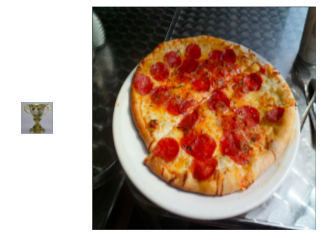
\includegraphics[width=1\textwidth]{recursos/imagens/results/dataset_diff.png}

    Fonte: do próprio autor.
\end{figure}

Adicionalmente, é relevante mencionar que, em amostras pequenas como as do conjunto de dados CIFAR 100, a quantidade de informação a ser preservada é mínima. Isso pode explicar o desempenho inferior do método BPCAPooling, embora não tenha representado uma barreira significativa para os métodos de \textit{pooling} tradicionais, tais como \textit{Max Pooling} e \textit{Avg Pooling}, uma vez que a preservação da espacialidade das amostras de entrada não é a principal preocupação desses métodos.

Além disso, conforme discutido na Seção \ref{results:class}, ao analisar o processo de \textit{fine-tuning} utilizando o método BPCAPooling, destaca-se um comportamento notável no quarto bloco convolucional, onde ocorre uma tendência ascendente na acurácia e uma tendência de redução no \textit{loss} ao longo das épocas de treinamento e validação. Essa tendência sugere que características espaciais importantes provavelmente estão sendo capturadas e retidas no quarto bloco convolucional. É notável que o modelo não apresenta sinais de \textit{overfitting} nesse bloco, indicando que mais épocas poderiam ser empregadas nessa etapa do processo para explorar melhor essa tendência ascendente. Contudo, é crucial considerar que a condução de épocas adicionais demandaria recursos computacionais significativos, devido à complexidade do método e ao custo computacional associado.

A representação da acurácia e \textit{loss} para o conjunto de dados CIFAR 100 está ilustrada nas Figuras \ref{results:fig:datasets:1} e \ref{results:fig:datasets:2}, respectivamente, enquanto as Figuras \ref{results:fig:datasets:3} e \ref{results:fig:datasets:4} mostram a evolução da acurácia e \textit{loss} para o conjunto de dados \textit{Food}-101, todas referentes ao uso do método BPCAPooling.


\begin{figure}[H]
    \centering
    \caption{Evolução de Acurácia no conjunto de dados CIFAR 100.}
    \label{results:fig:datasets:1}
     \begin{subfigure}[t]{0.45\textwidth}
         \centering
         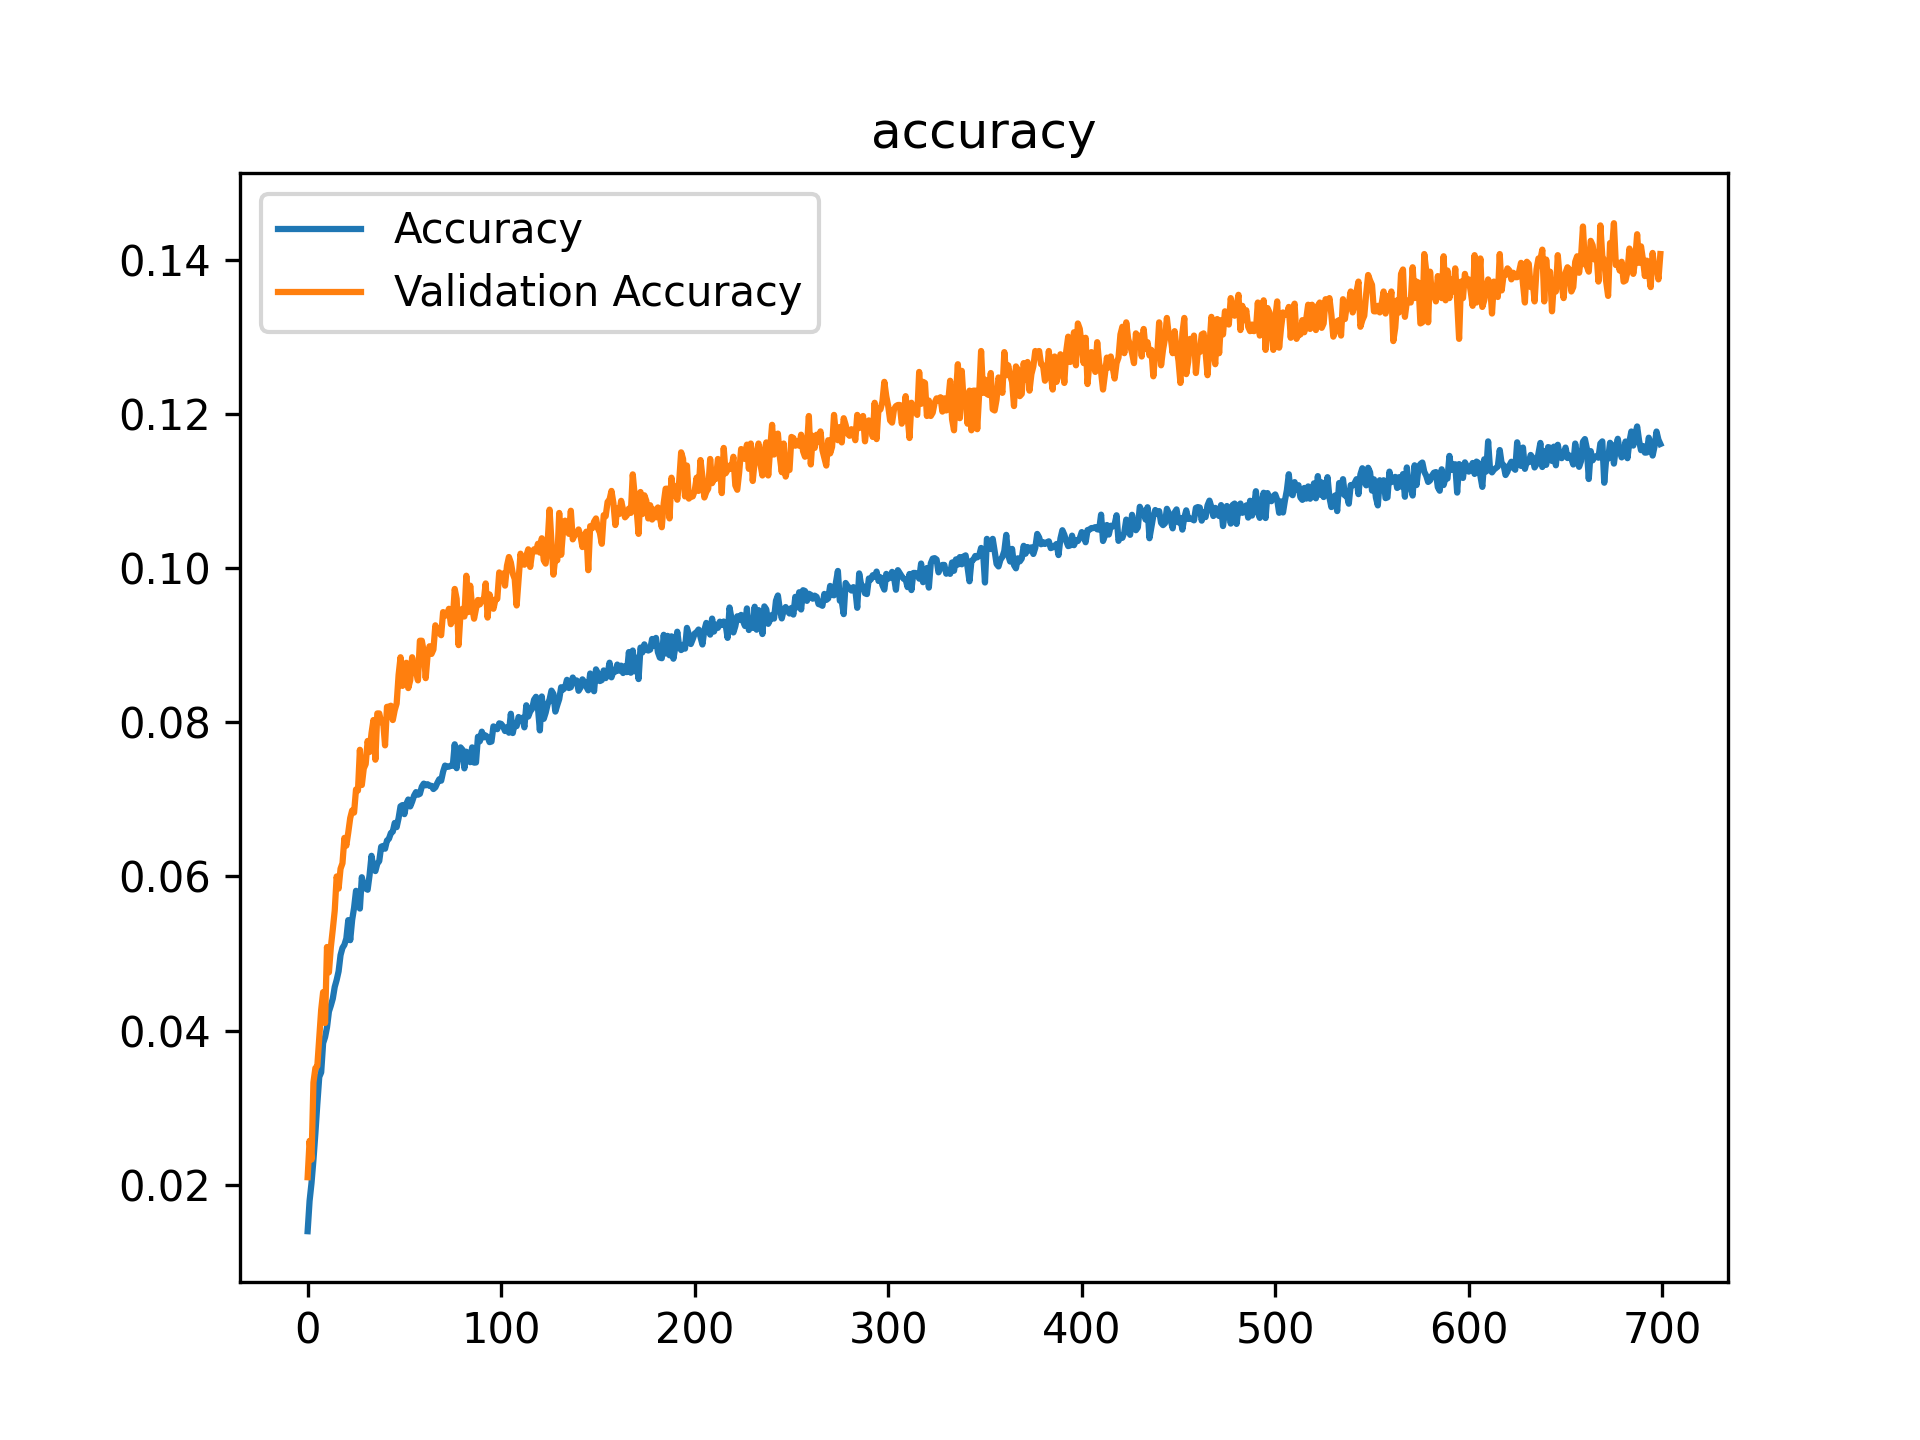
\includegraphics[width=1\linewidth]{recursos/imagens/results/cifar_wp_accuracy.png}
         \caption{Aquecimento.}
         \label{results:fig:datasets:1.1}
     \end{subfigure}%
     ~ 
     \begin{subfigure}[t]{0.45\textwidth}
         \centering
         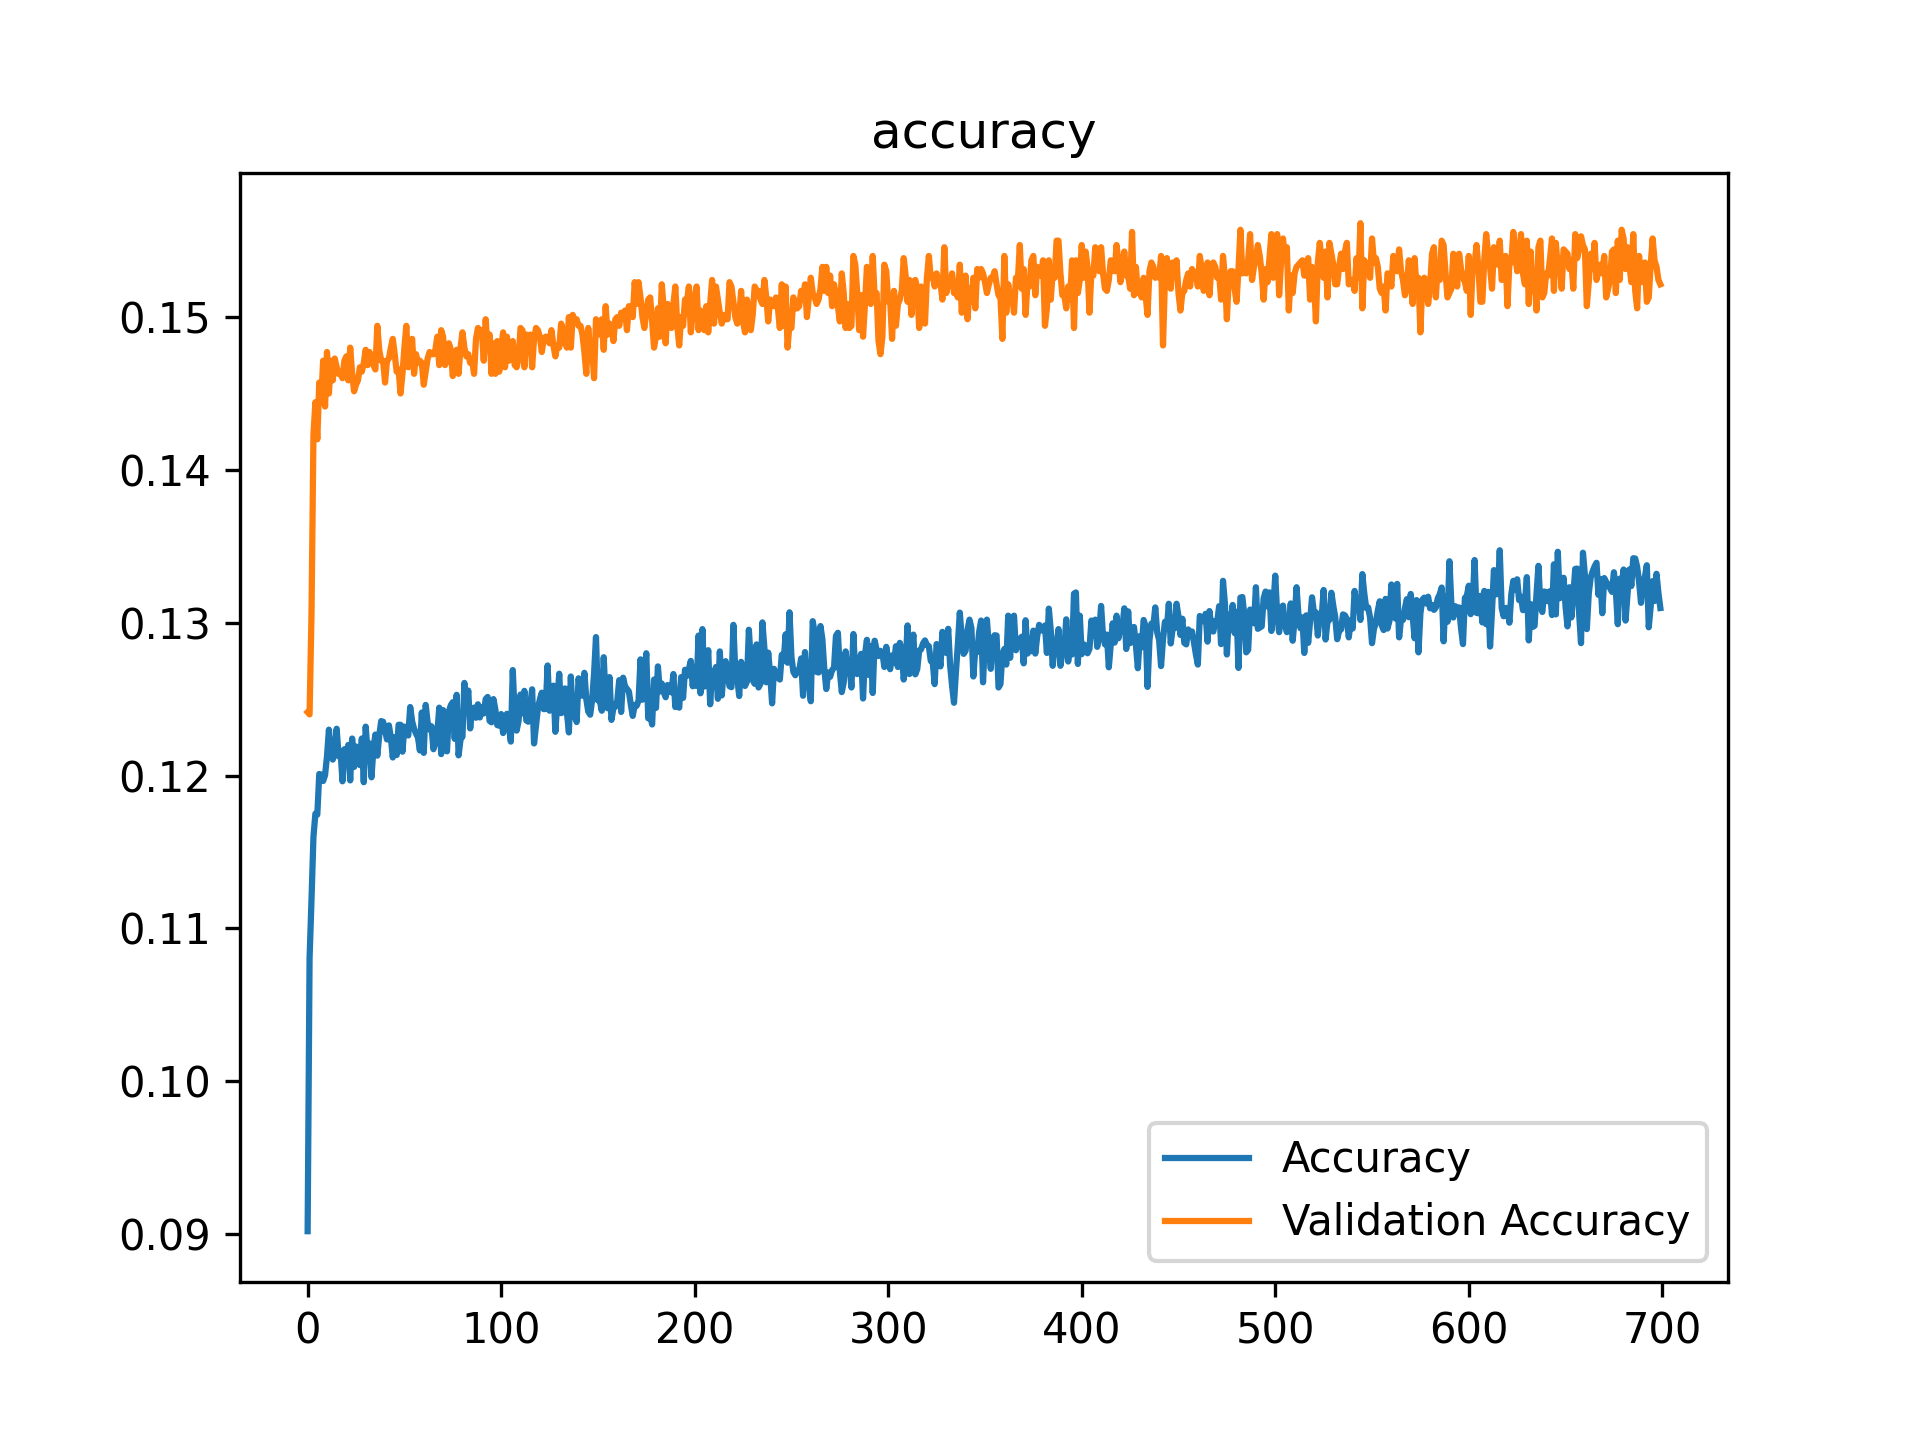
\includegraphics[width=1\linewidth]{recursos/imagens/results/cifar_accuracy1.png}
         \caption{Bloco 5.}
         \label{results:fig:datasets:1.2}
     \end{subfigure}%
     ~ 
     
     \begin{subfigure}[t]{0.45\textwidth}
         \centering
         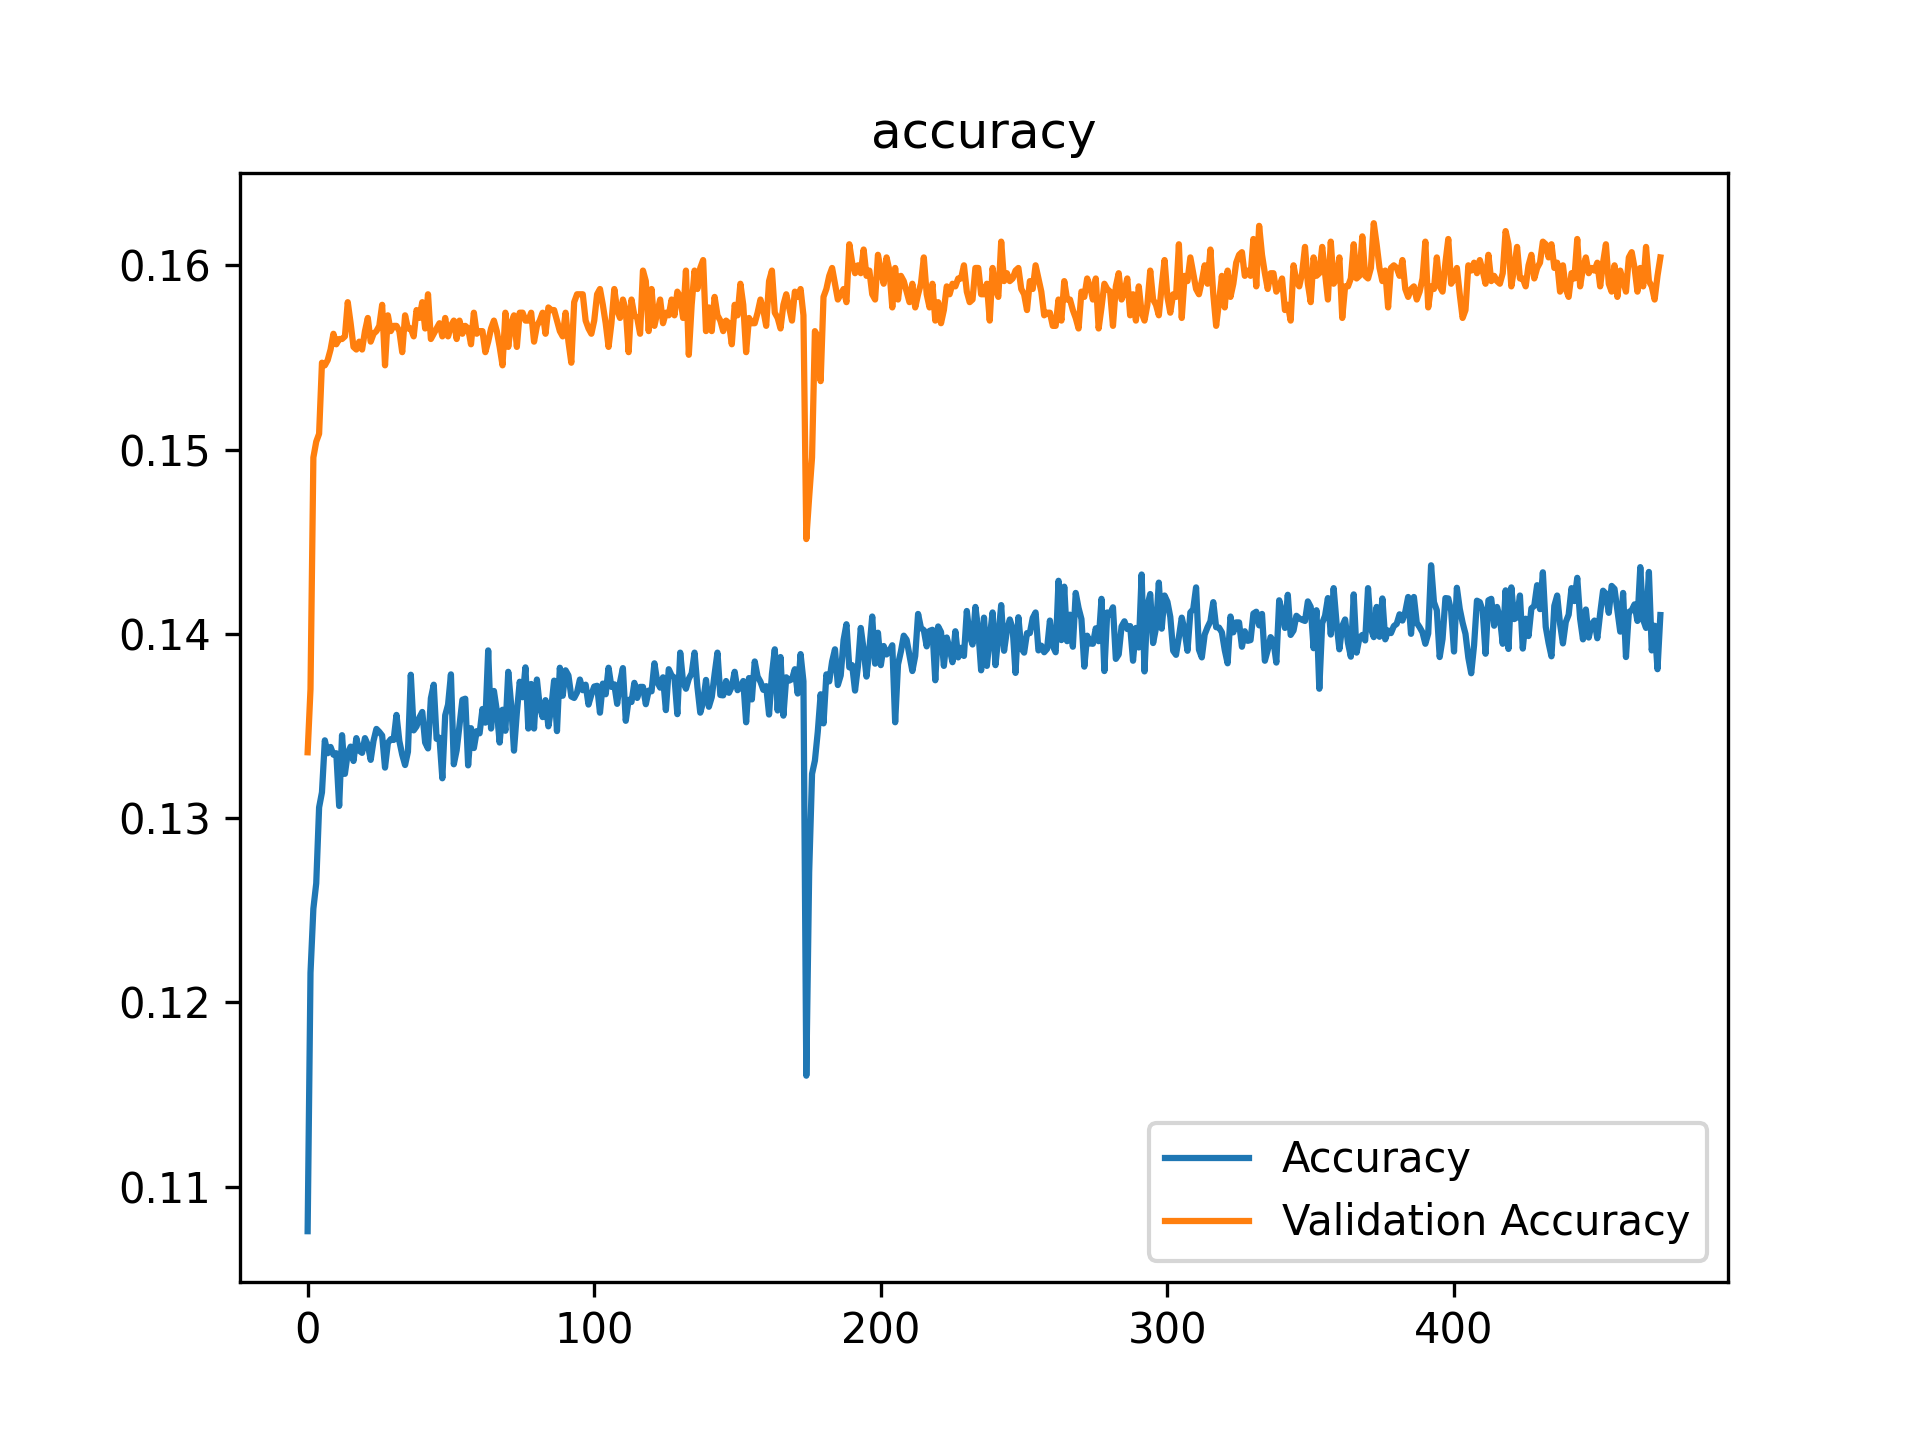
\includegraphics[width=1\linewidth]{recursos/imagens/results/cifar_accuracy2.png}
         \caption{Bloco 4.}
         \label{results:fig:datasets:1.3}
     \end{subfigure}
     ~
     \begin{subfigure}[t]{0.45\textwidth}
         \centering
         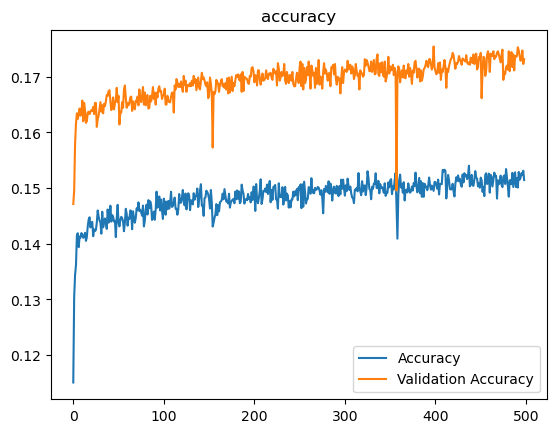
\includegraphics[width=1\linewidth]{recursos/imagens/results/cifar_accuracy3.png}
         \caption{Bloco 3.}
         \label{results:fig:datasets:1.4}
     \end{subfigure}
     
     Fonte: do próprio autor.
 \end{figure}

\begin{figure}[H]
    \centering
    \caption{Evolução de \textit{Loss} no conjunto de dados CIFAR 100.}
    \label{results:fig:datasets:2}
     \begin{subfigure}[t]{0.45\textwidth}
         \centering
         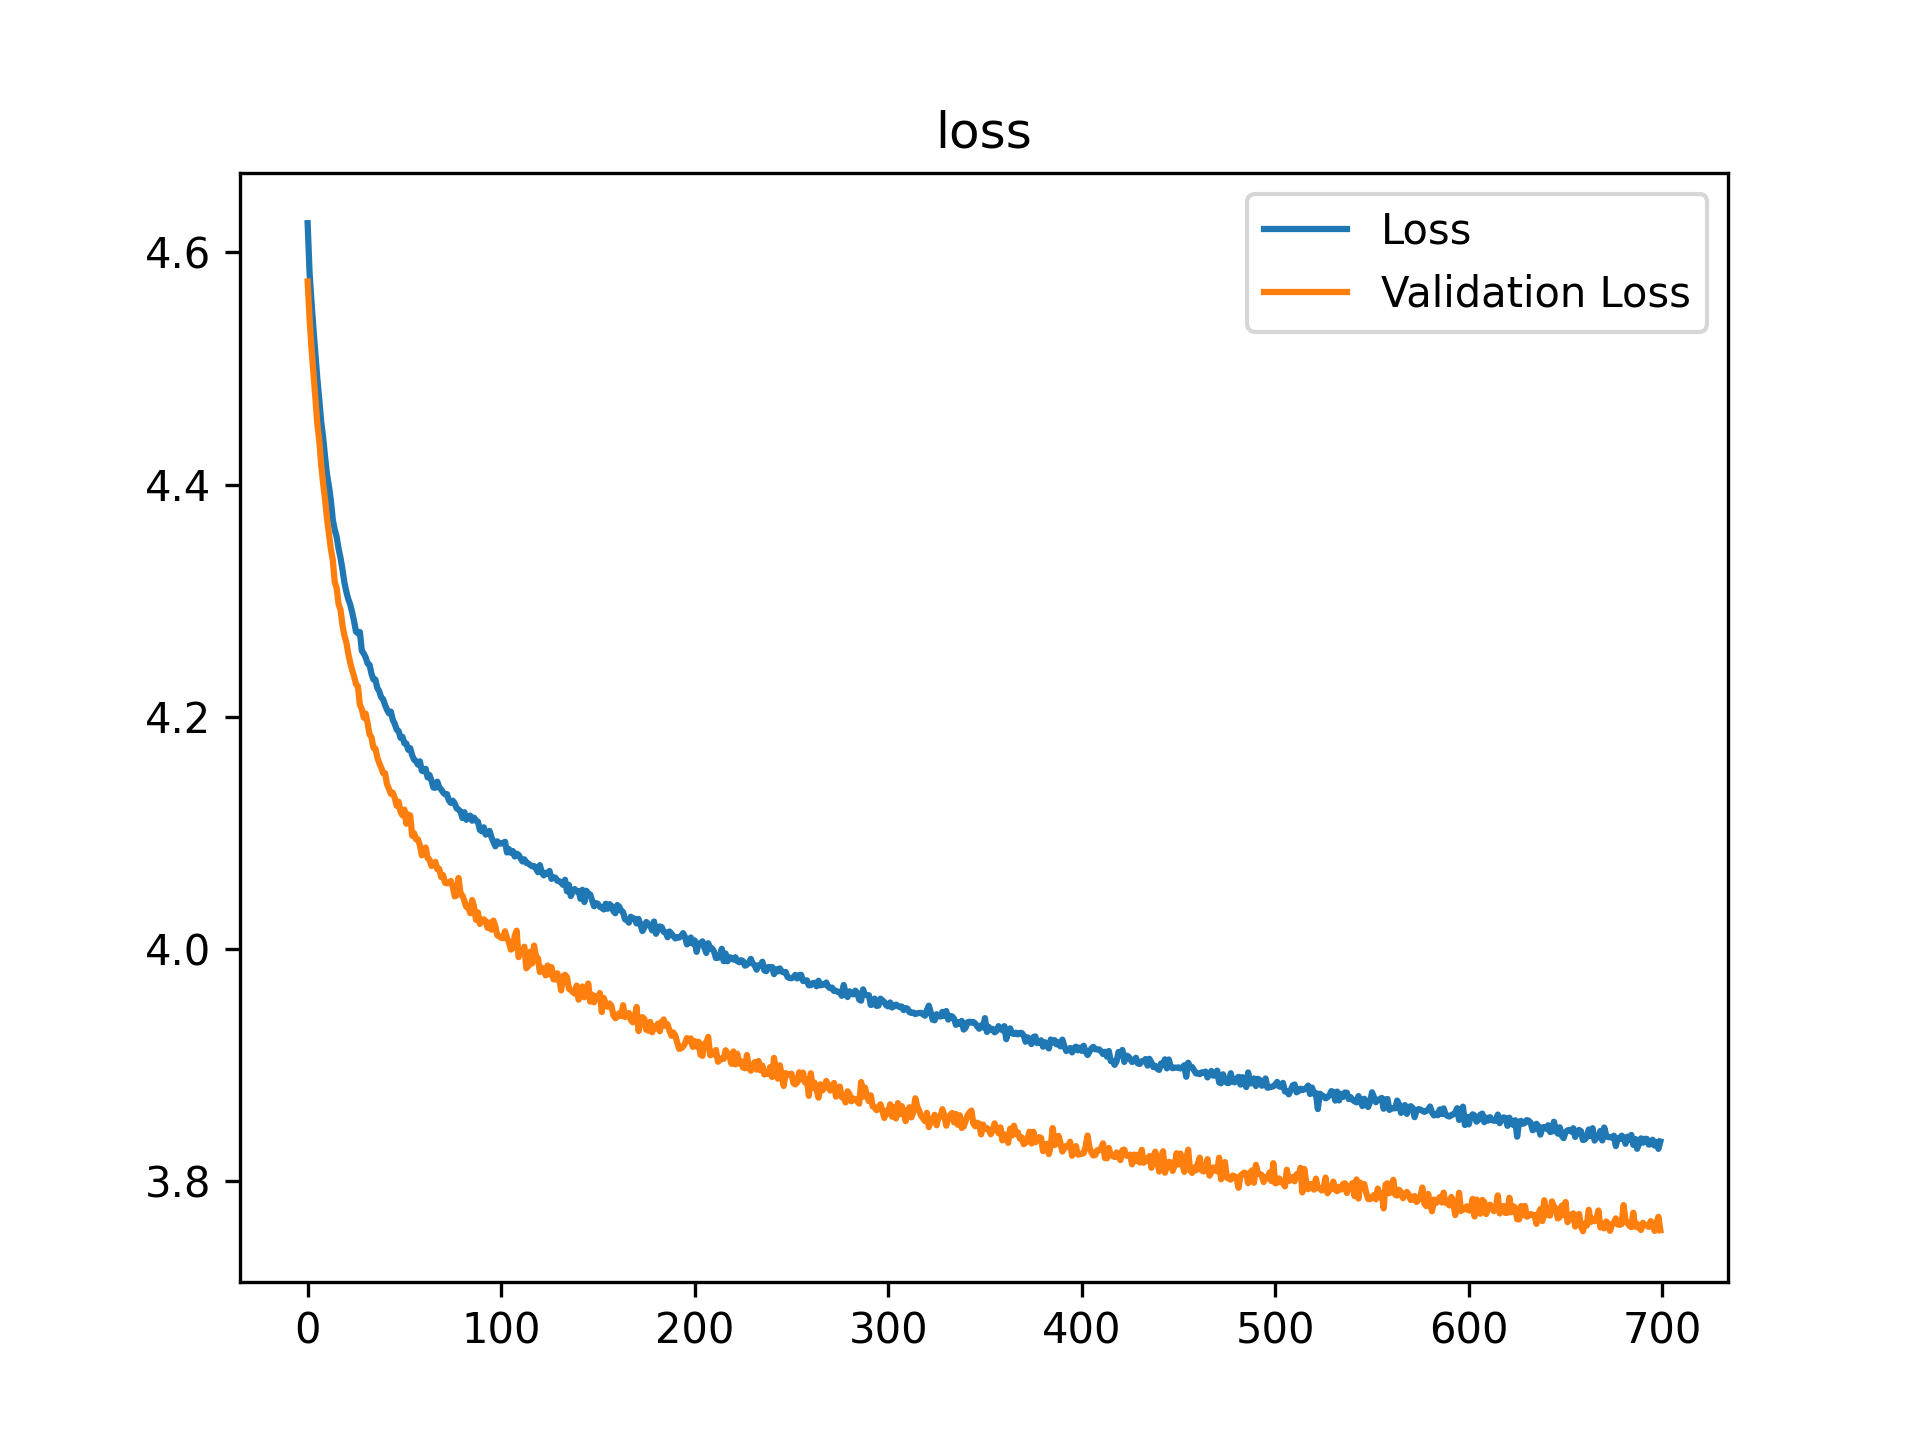
\includegraphics[width=1\linewidth]{recursos/imagens/results/cifar_wp_loss.png}
         \caption{Aquecimento.}
         \label{results:fig:datasets:2.1}
     \end{subfigure}%
     ~ 
     \begin{subfigure}[t]{0.45\textwidth}
         \centering
         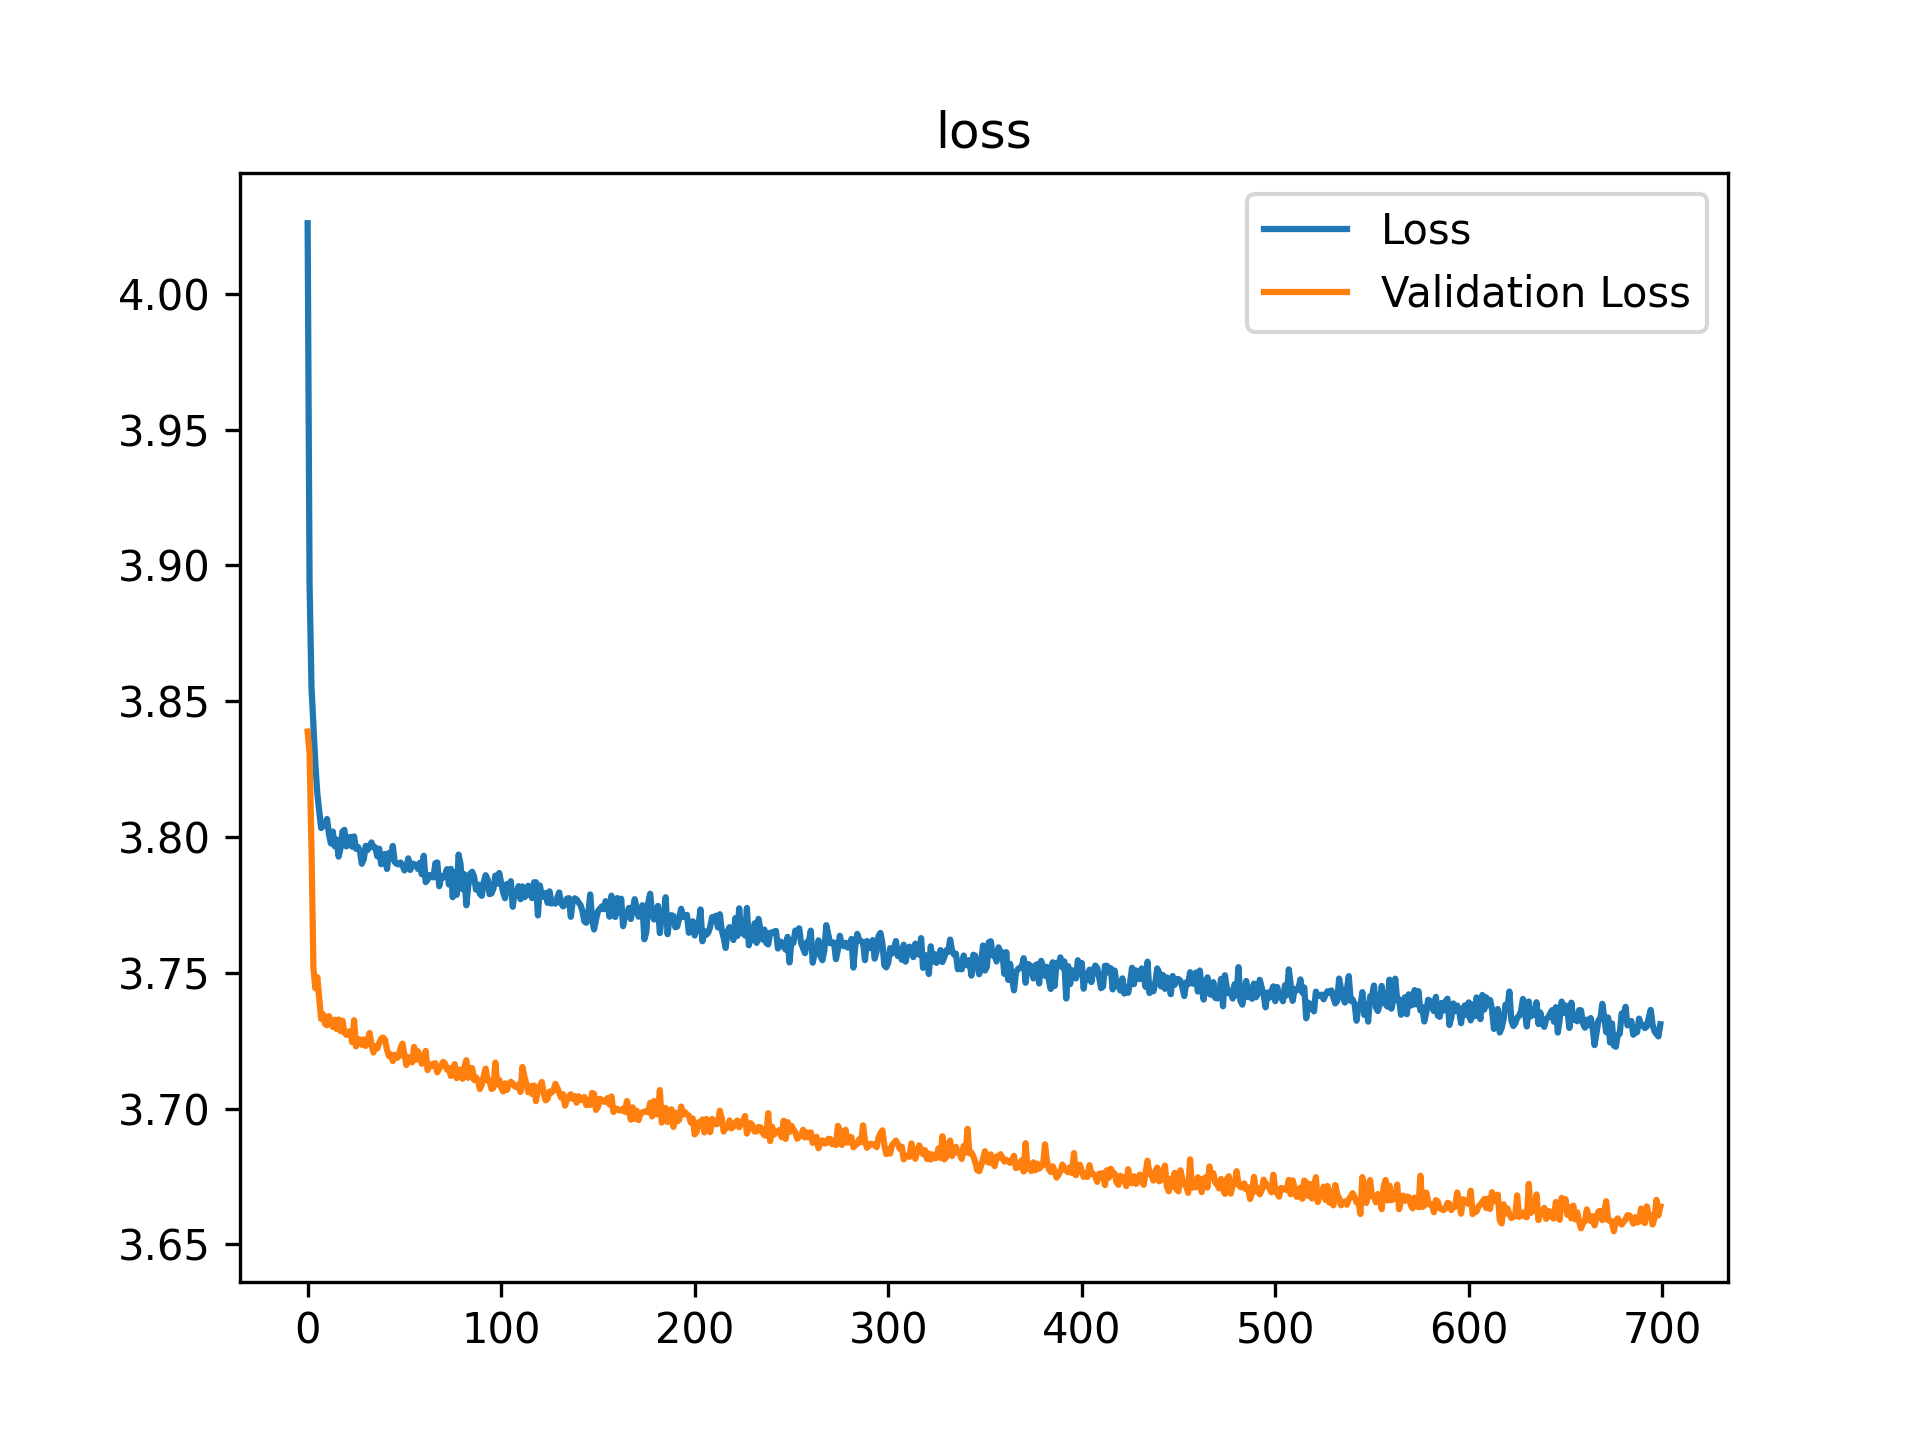
\includegraphics[width=1\linewidth]{recursos/imagens/results/cifar_loss1.png}
         \caption{Bloco 5.}
         \label{results:fig:datasets:2.2}
     \end{subfigure}%
     ~ 
     
     \begin{subfigure}[t]{0.45\textwidth}
         \centering
         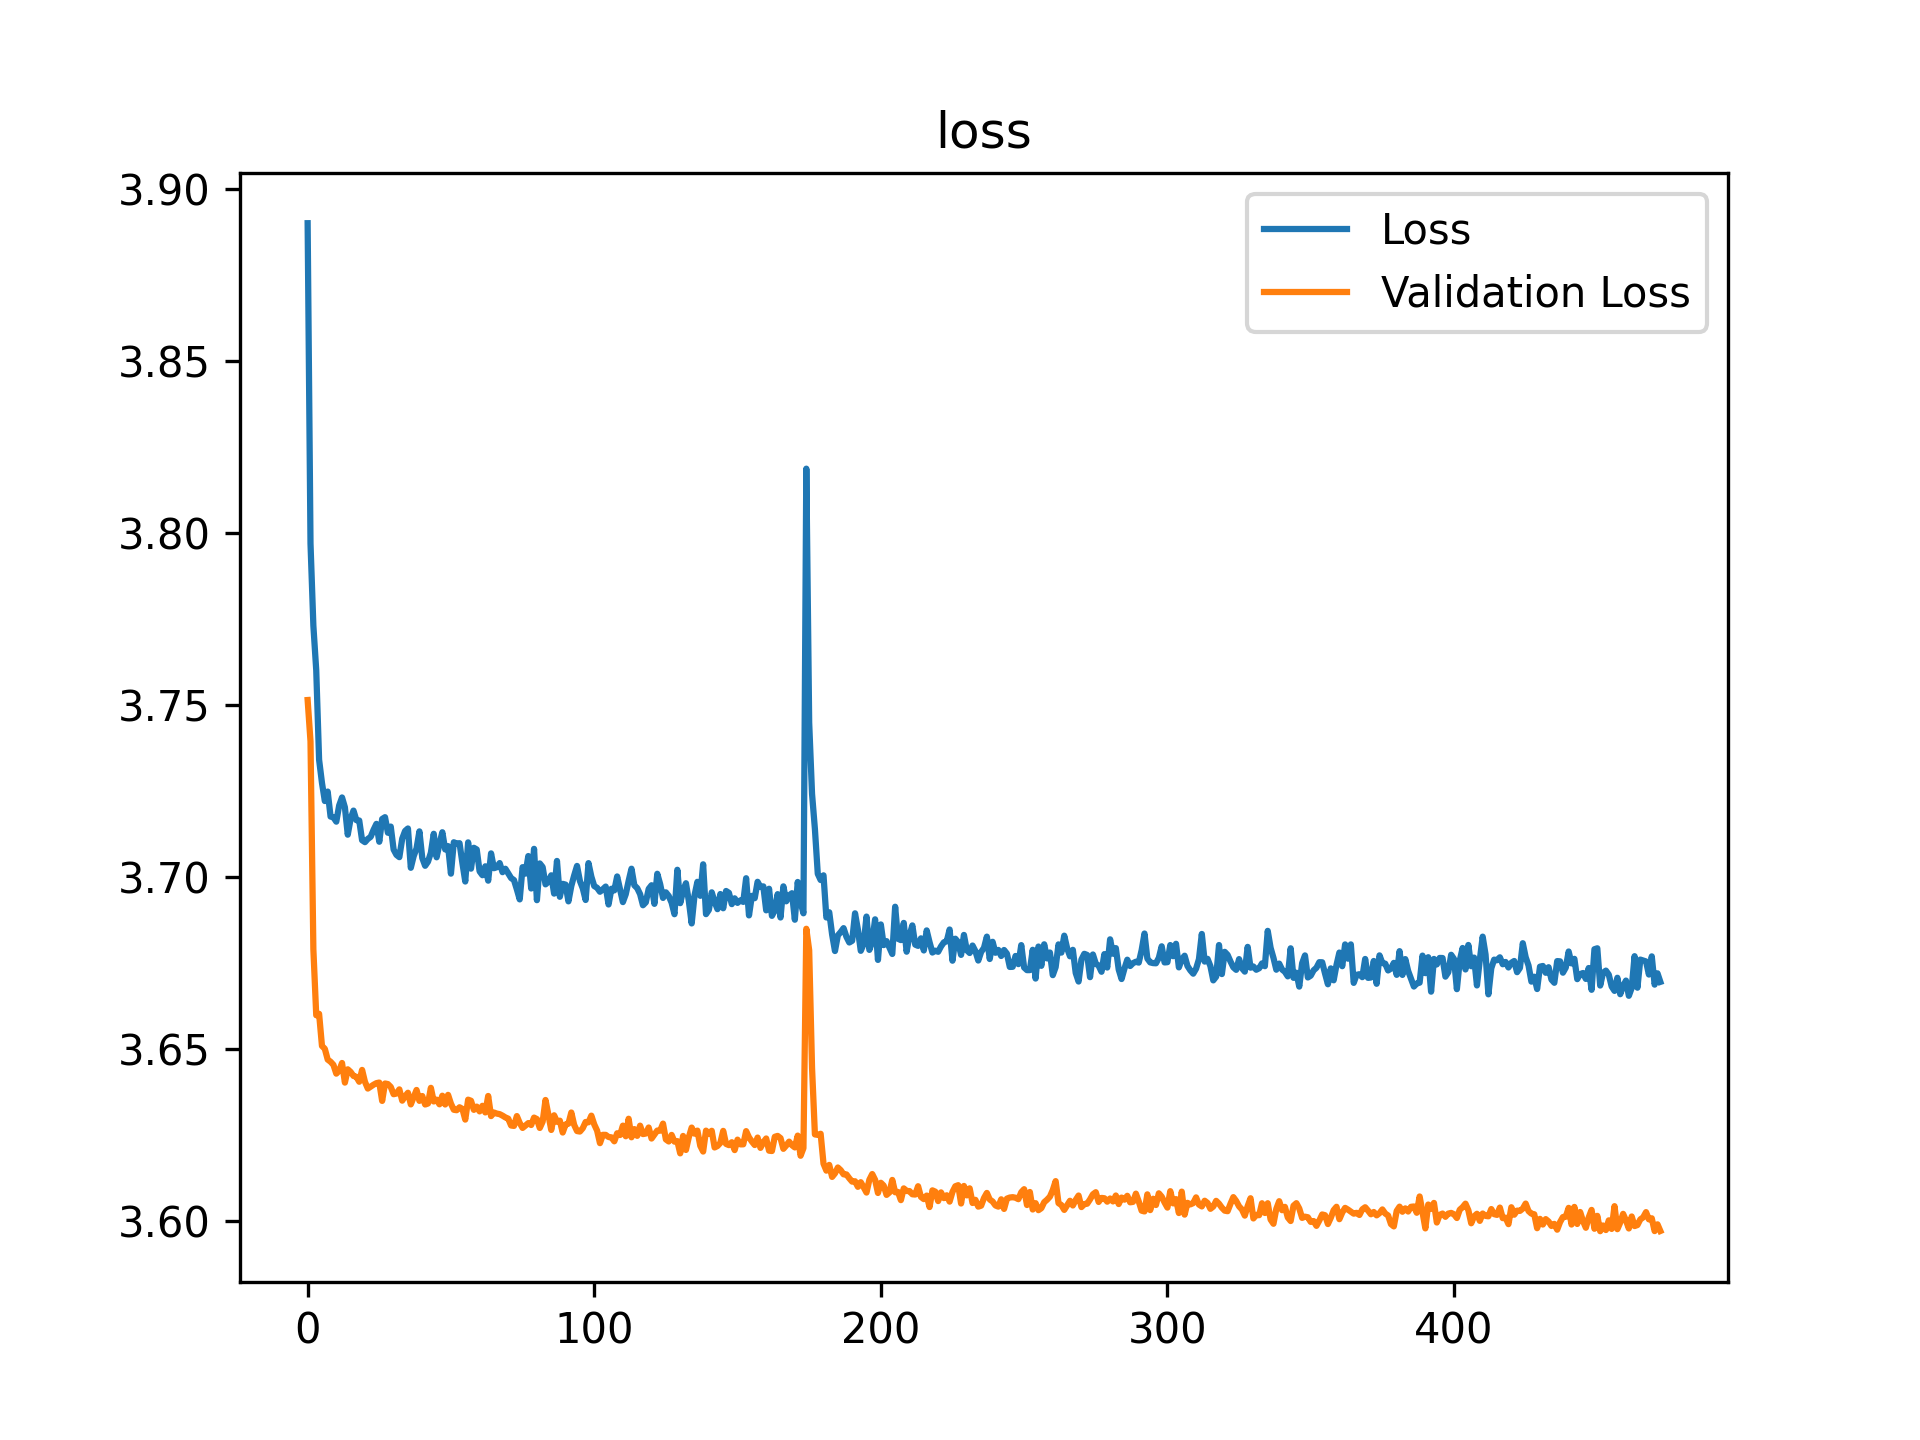
\includegraphics[width=1\linewidth]{recursos/imagens/results/cifar_loss2.png}
         \caption{Bloco 4.}
         \label{results:fig:datasets:2.3}
     \end{subfigure}
     ~
     \begin{subfigure}[t]{0.45\textwidth}
         \centering
         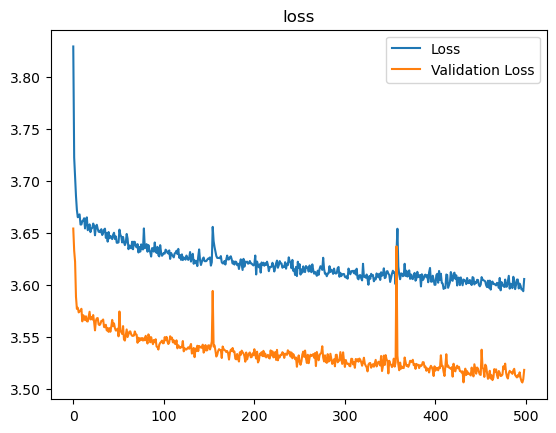
\includegraphics[width=1\linewidth]{recursos/imagens/results/cifar_loss3.png}
         \caption{Bloco 3.}
         \label{results:fig:datasets:2.4}
     \end{subfigure}
     
     Fonte: do próprio autor.
 \end{figure}


\begin{figure}[H]
    \centering
    \caption{Evolução de Acurácia no conjunto de dados \textit{Food}-101.}
    \label{results:fig:datasets:3}
     \begin{subfigure}[t]{0.45\textwidth}
         \centering
         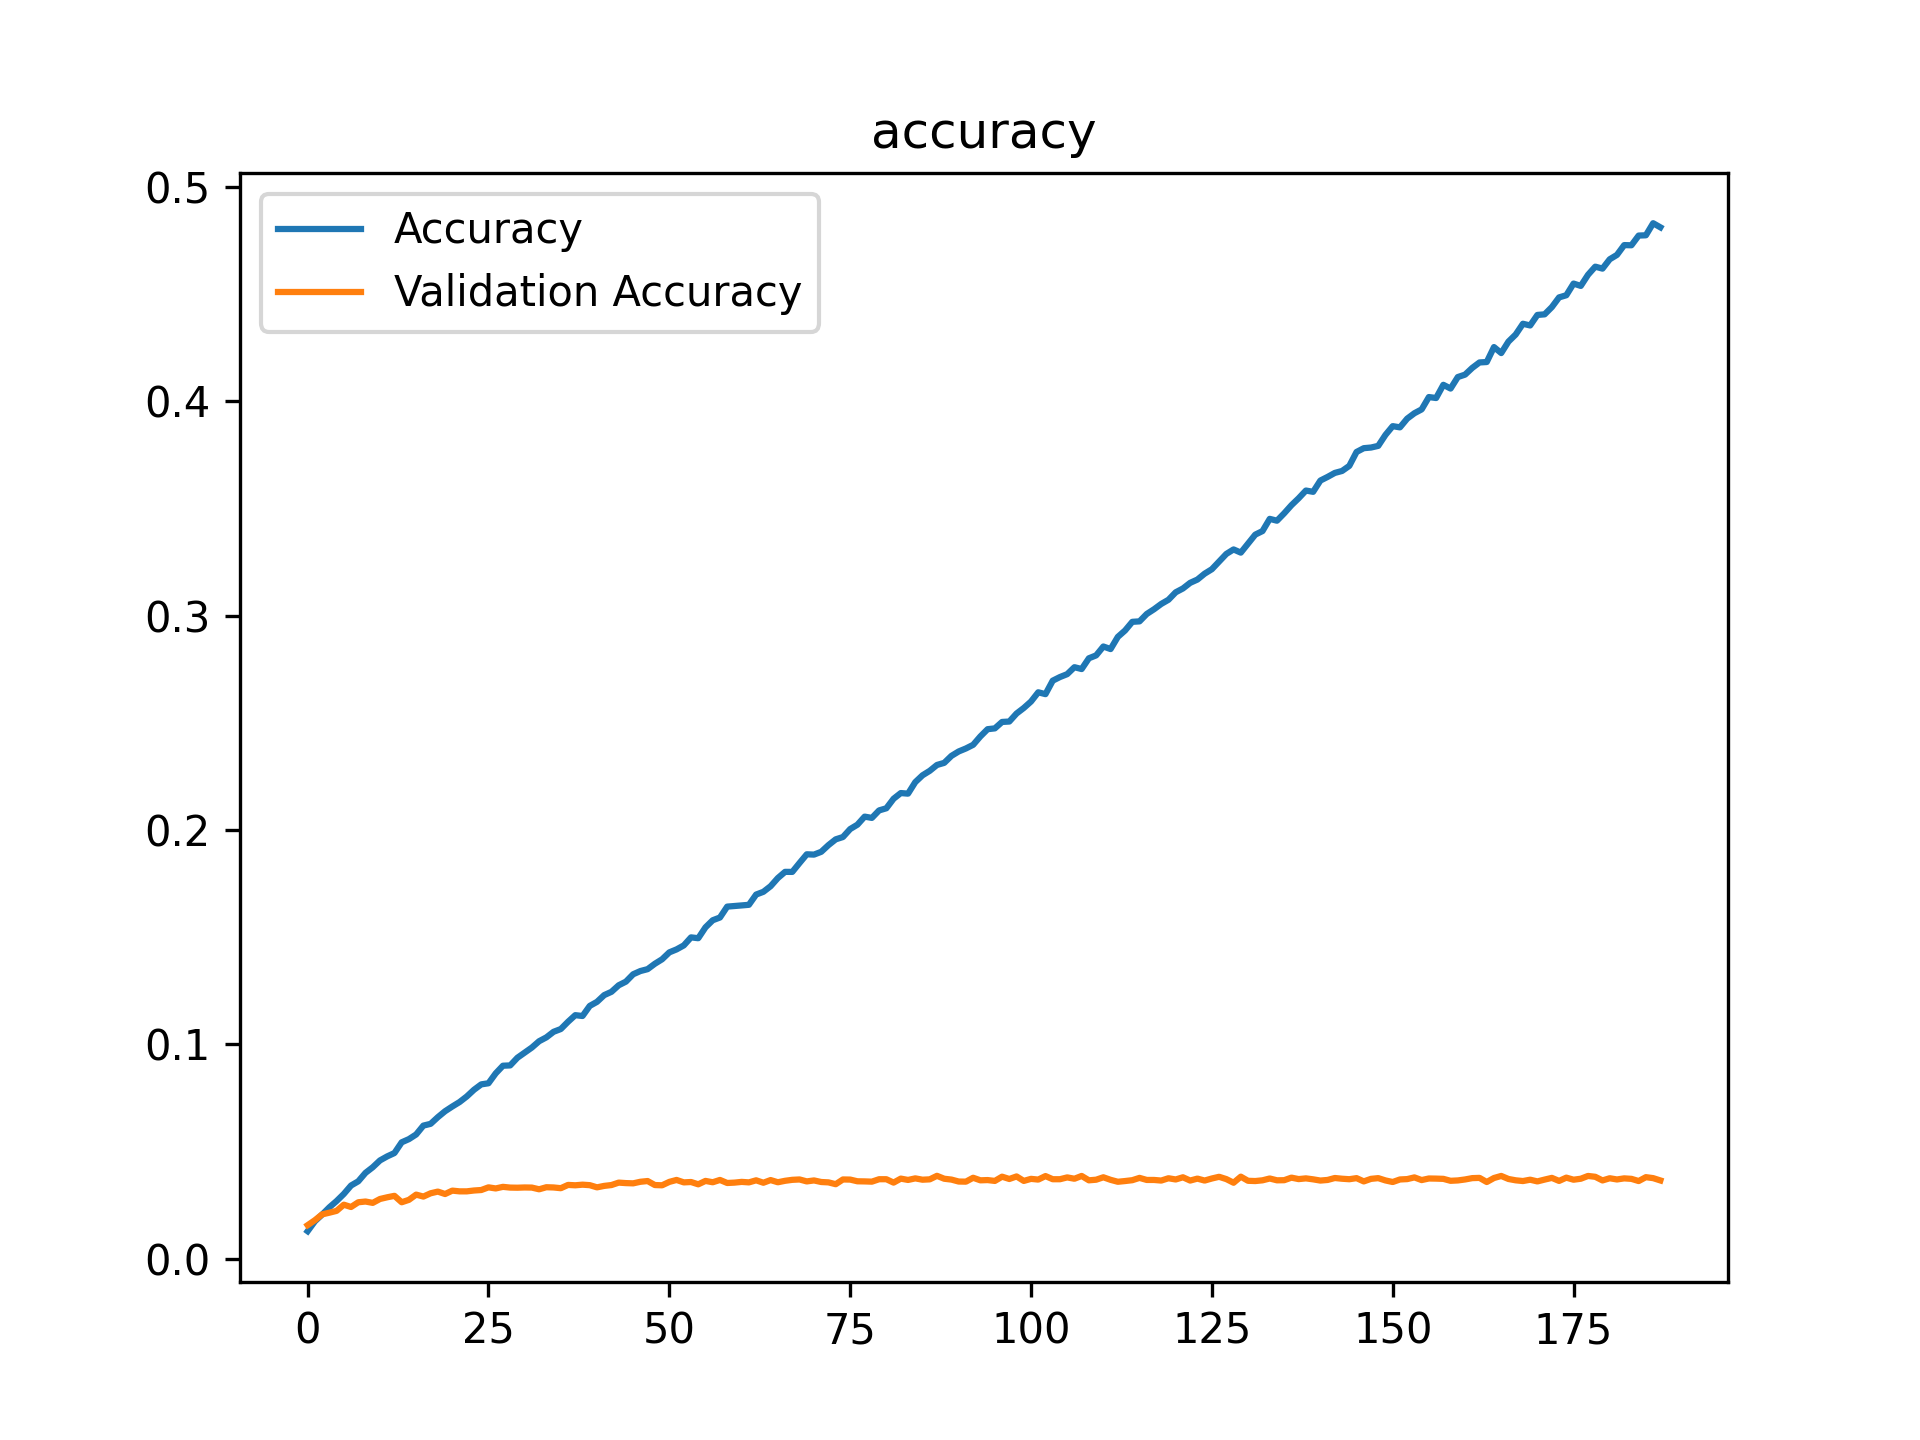
\includegraphics[width=1\linewidth]{recursos/imagens/results/food_wp_accuracy.png}
         \caption{Aquecimento.}
         \label{results:fig:datasets:3.1}
     \end{subfigure}%
     ~ 
     \begin{subfigure}[t]{0.45\textwidth}
         \centering
         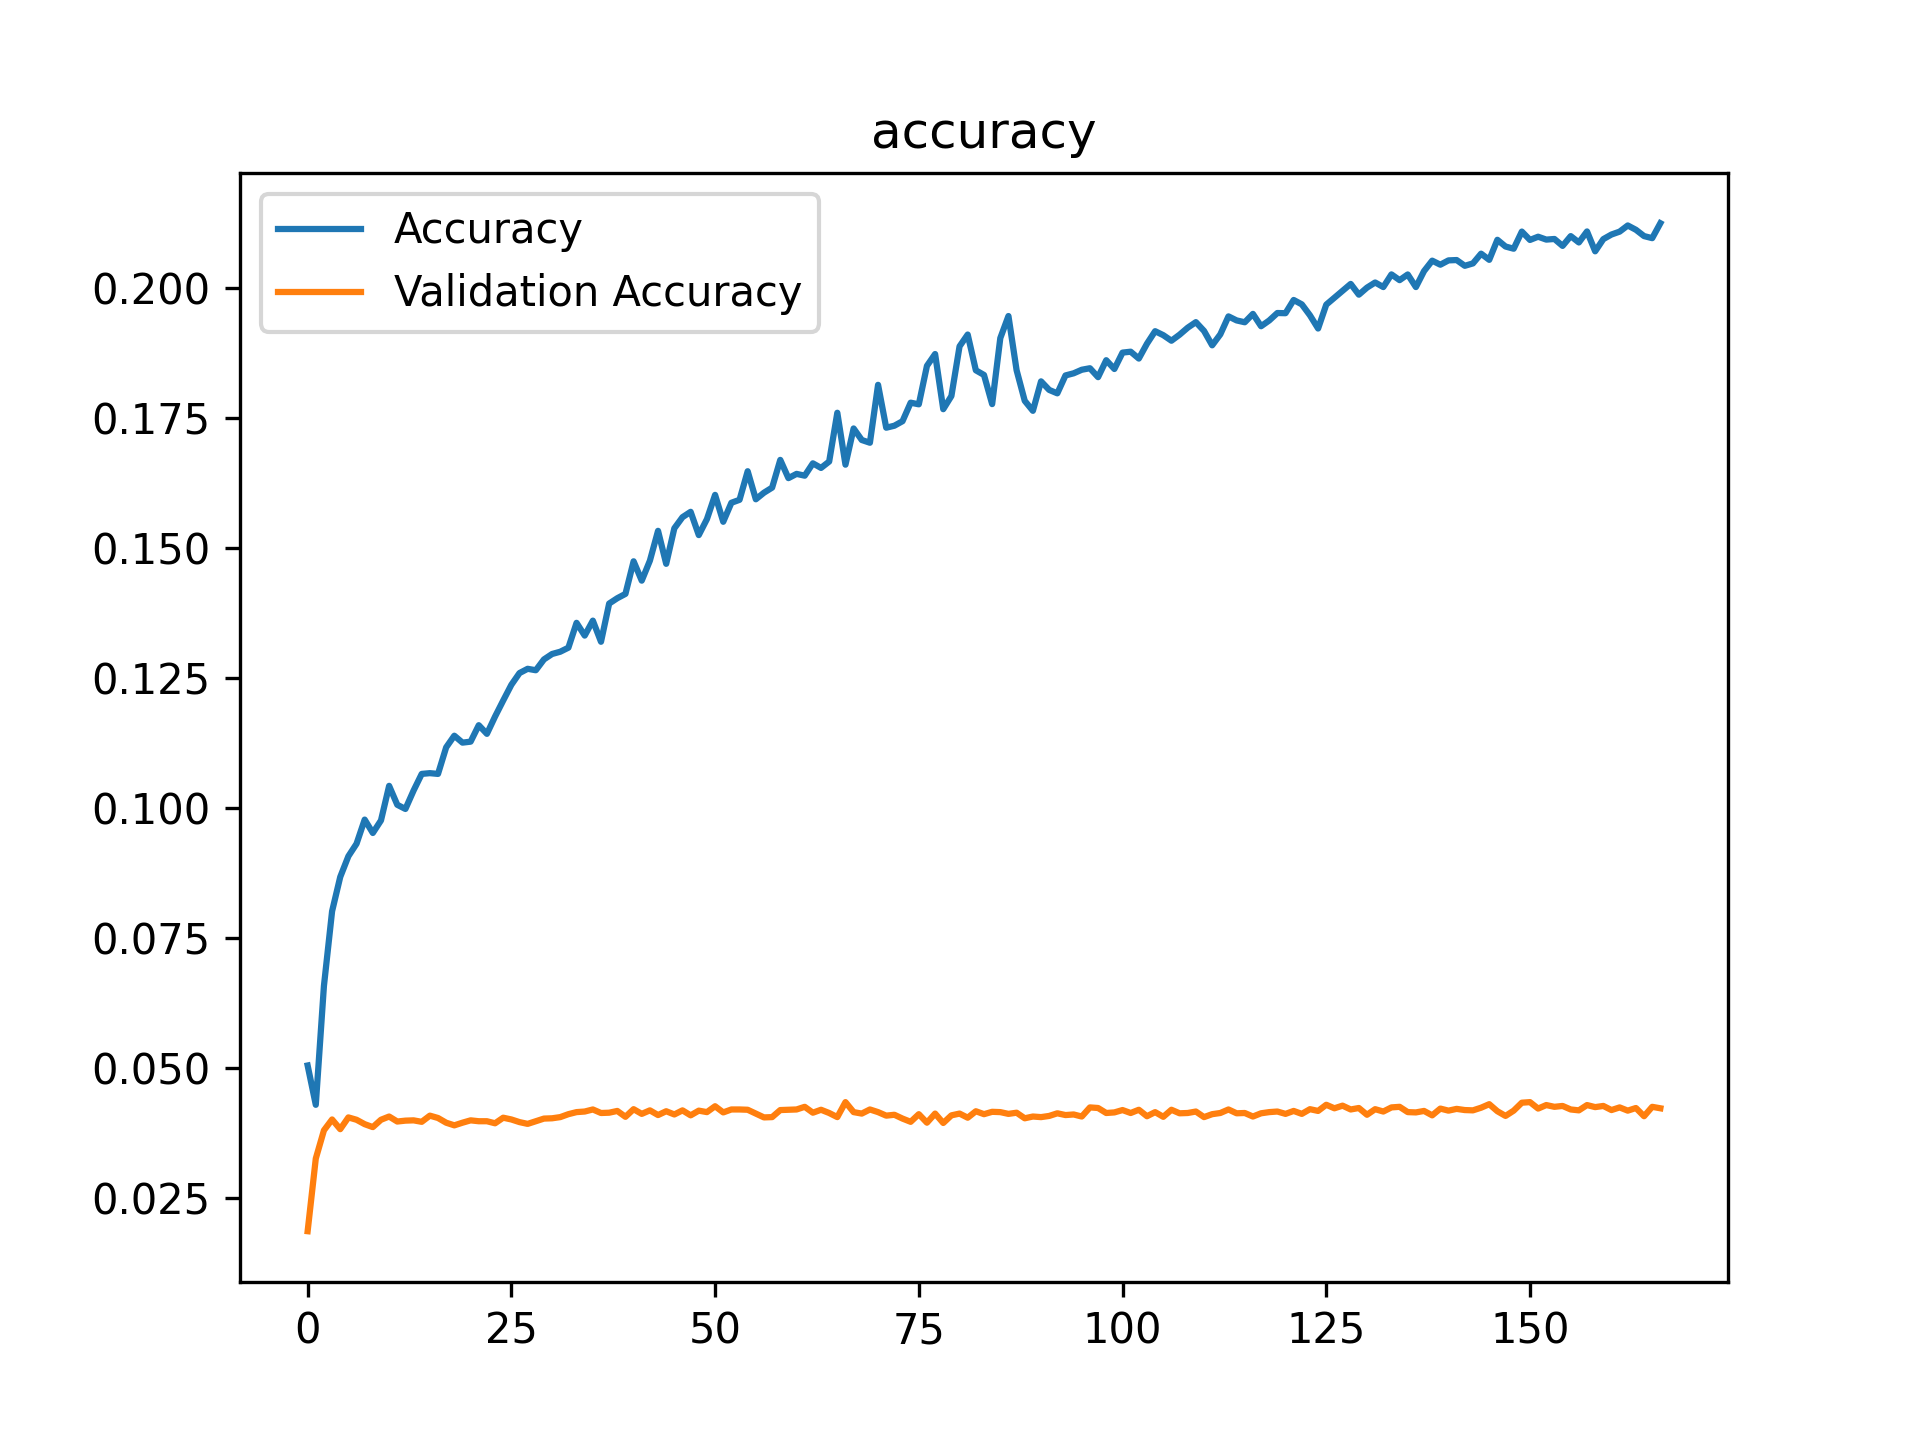
\includegraphics[width=1\linewidth]{recursos/imagens/results/food_accuracy1.png}
         \caption{Bloco 5.}
         \label{results:fig:datasets:3.2}
     \end{subfigure}%
     ~ 
     
     \begin{subfigure}[t]{0.45\textwidth}
         \centering
         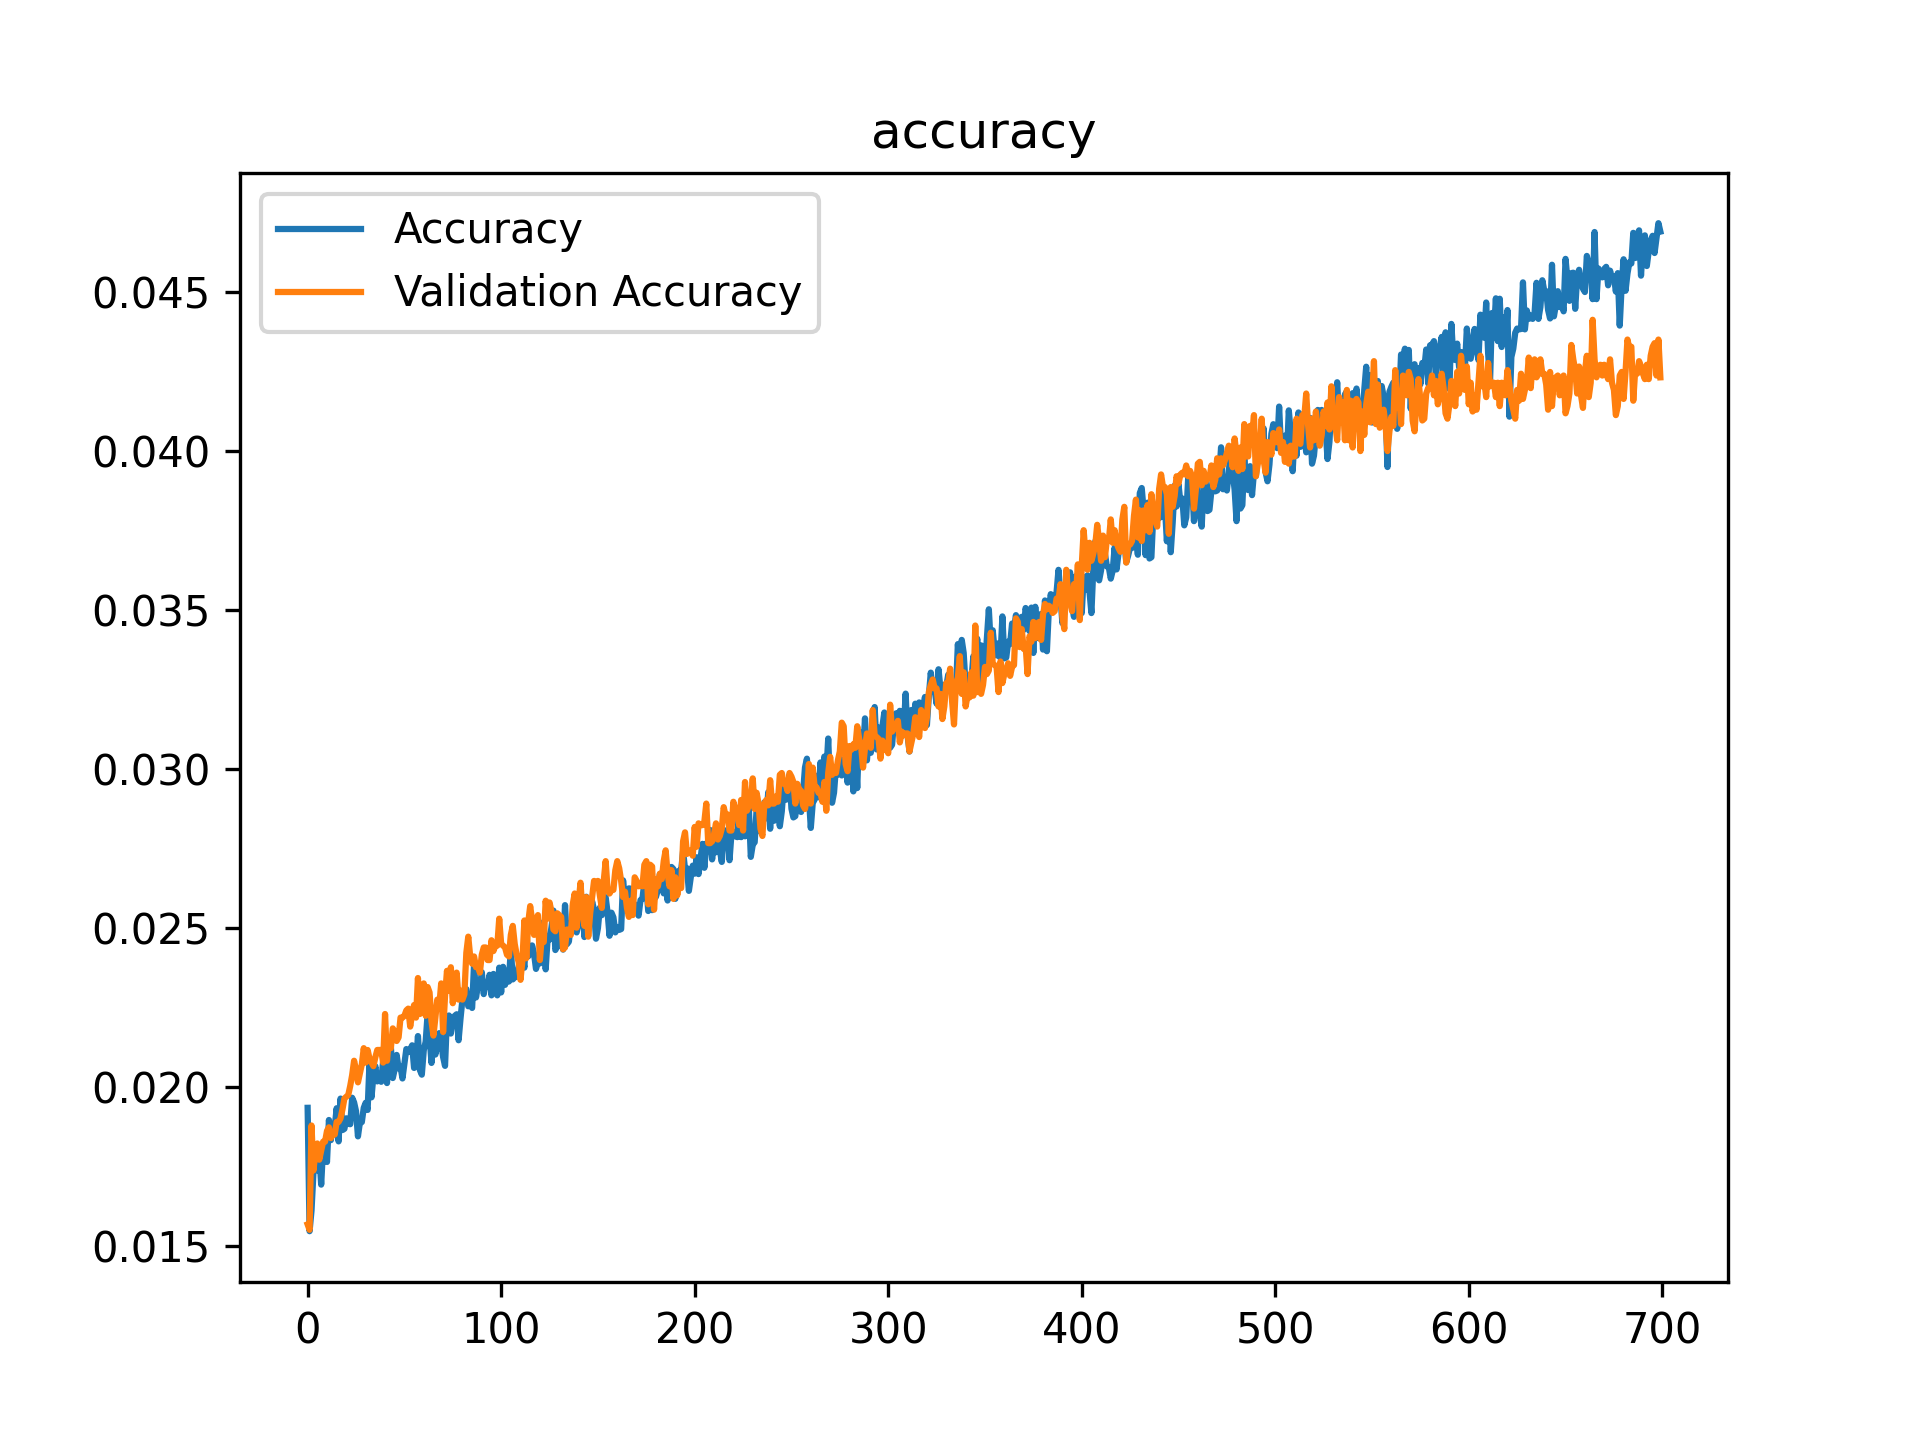
\includegraphics[width=1\linewidth]{recursos/imagens/results/food_accuracy2.png}
         \caption{Bloco 4.}
         \label{results:fig:datasets:3.3}
     \end{subfigure}
     ~
     \begin{subfigure}[t]{0.45\textwidth}
         \centering
         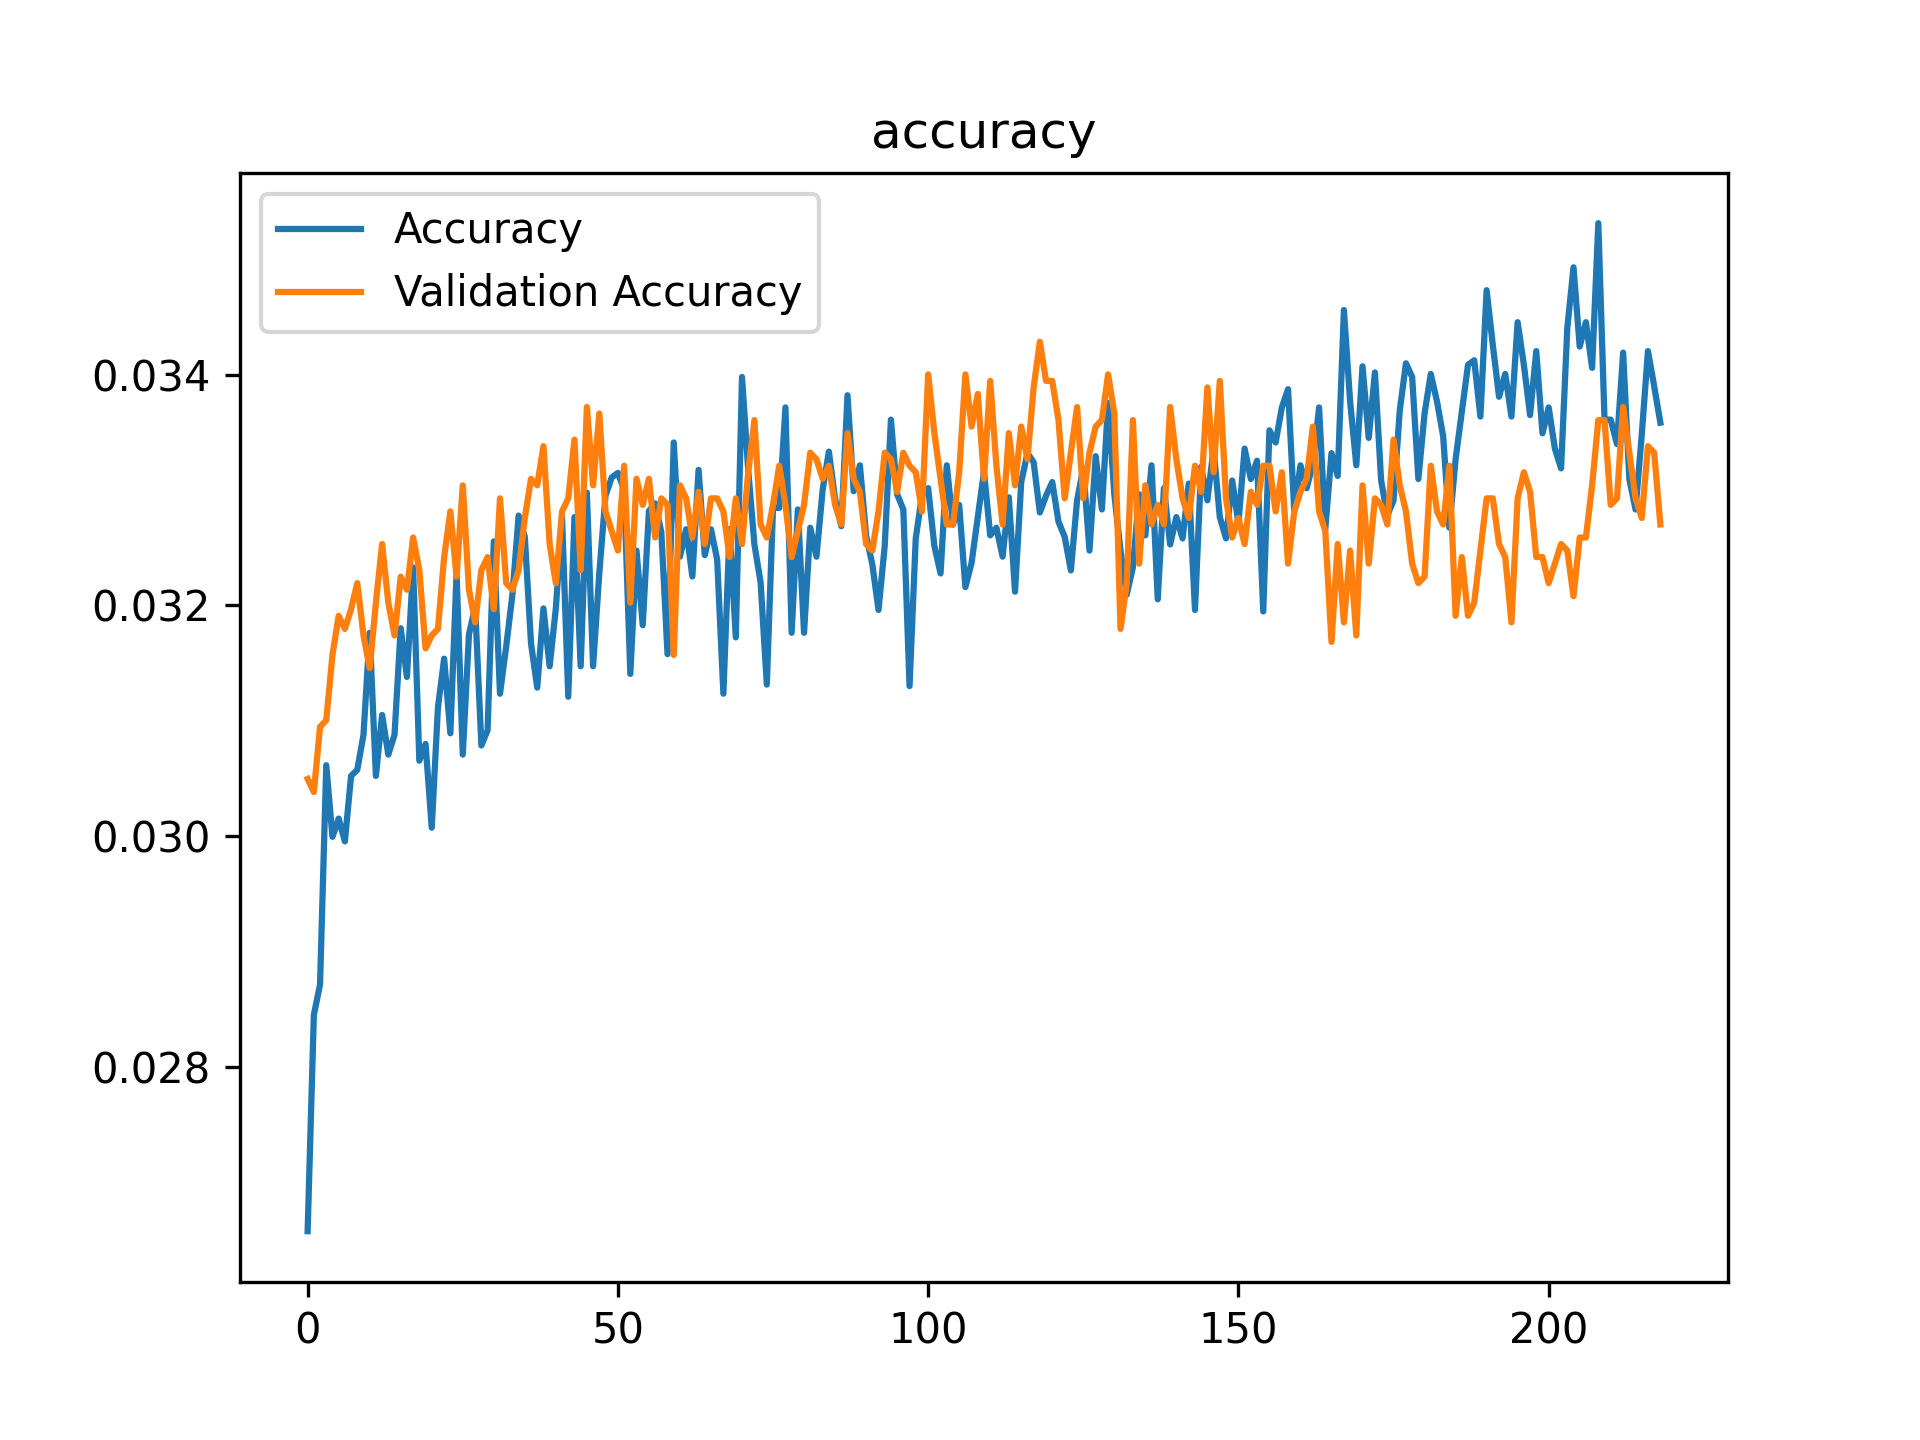
\includegraphics[width=1\linewidth]{recursos/imagens/results/food_accuracy3.png}
         \caption{Bloco 3.}
         \label{results:fig:datasets:3.4}
     \end{subfigure}
     
     Fonte: do próprio autor.
 \end{figure}

\begin{figure}[H]
    \centering
    \caption{Evolução da \textit{Loss} no conjunto de dados \textit{Food}-101.}
    \label{results:fig:datasets:4}
     \begin{subfigure}[t]{0.45\textwidth}
         \centering
         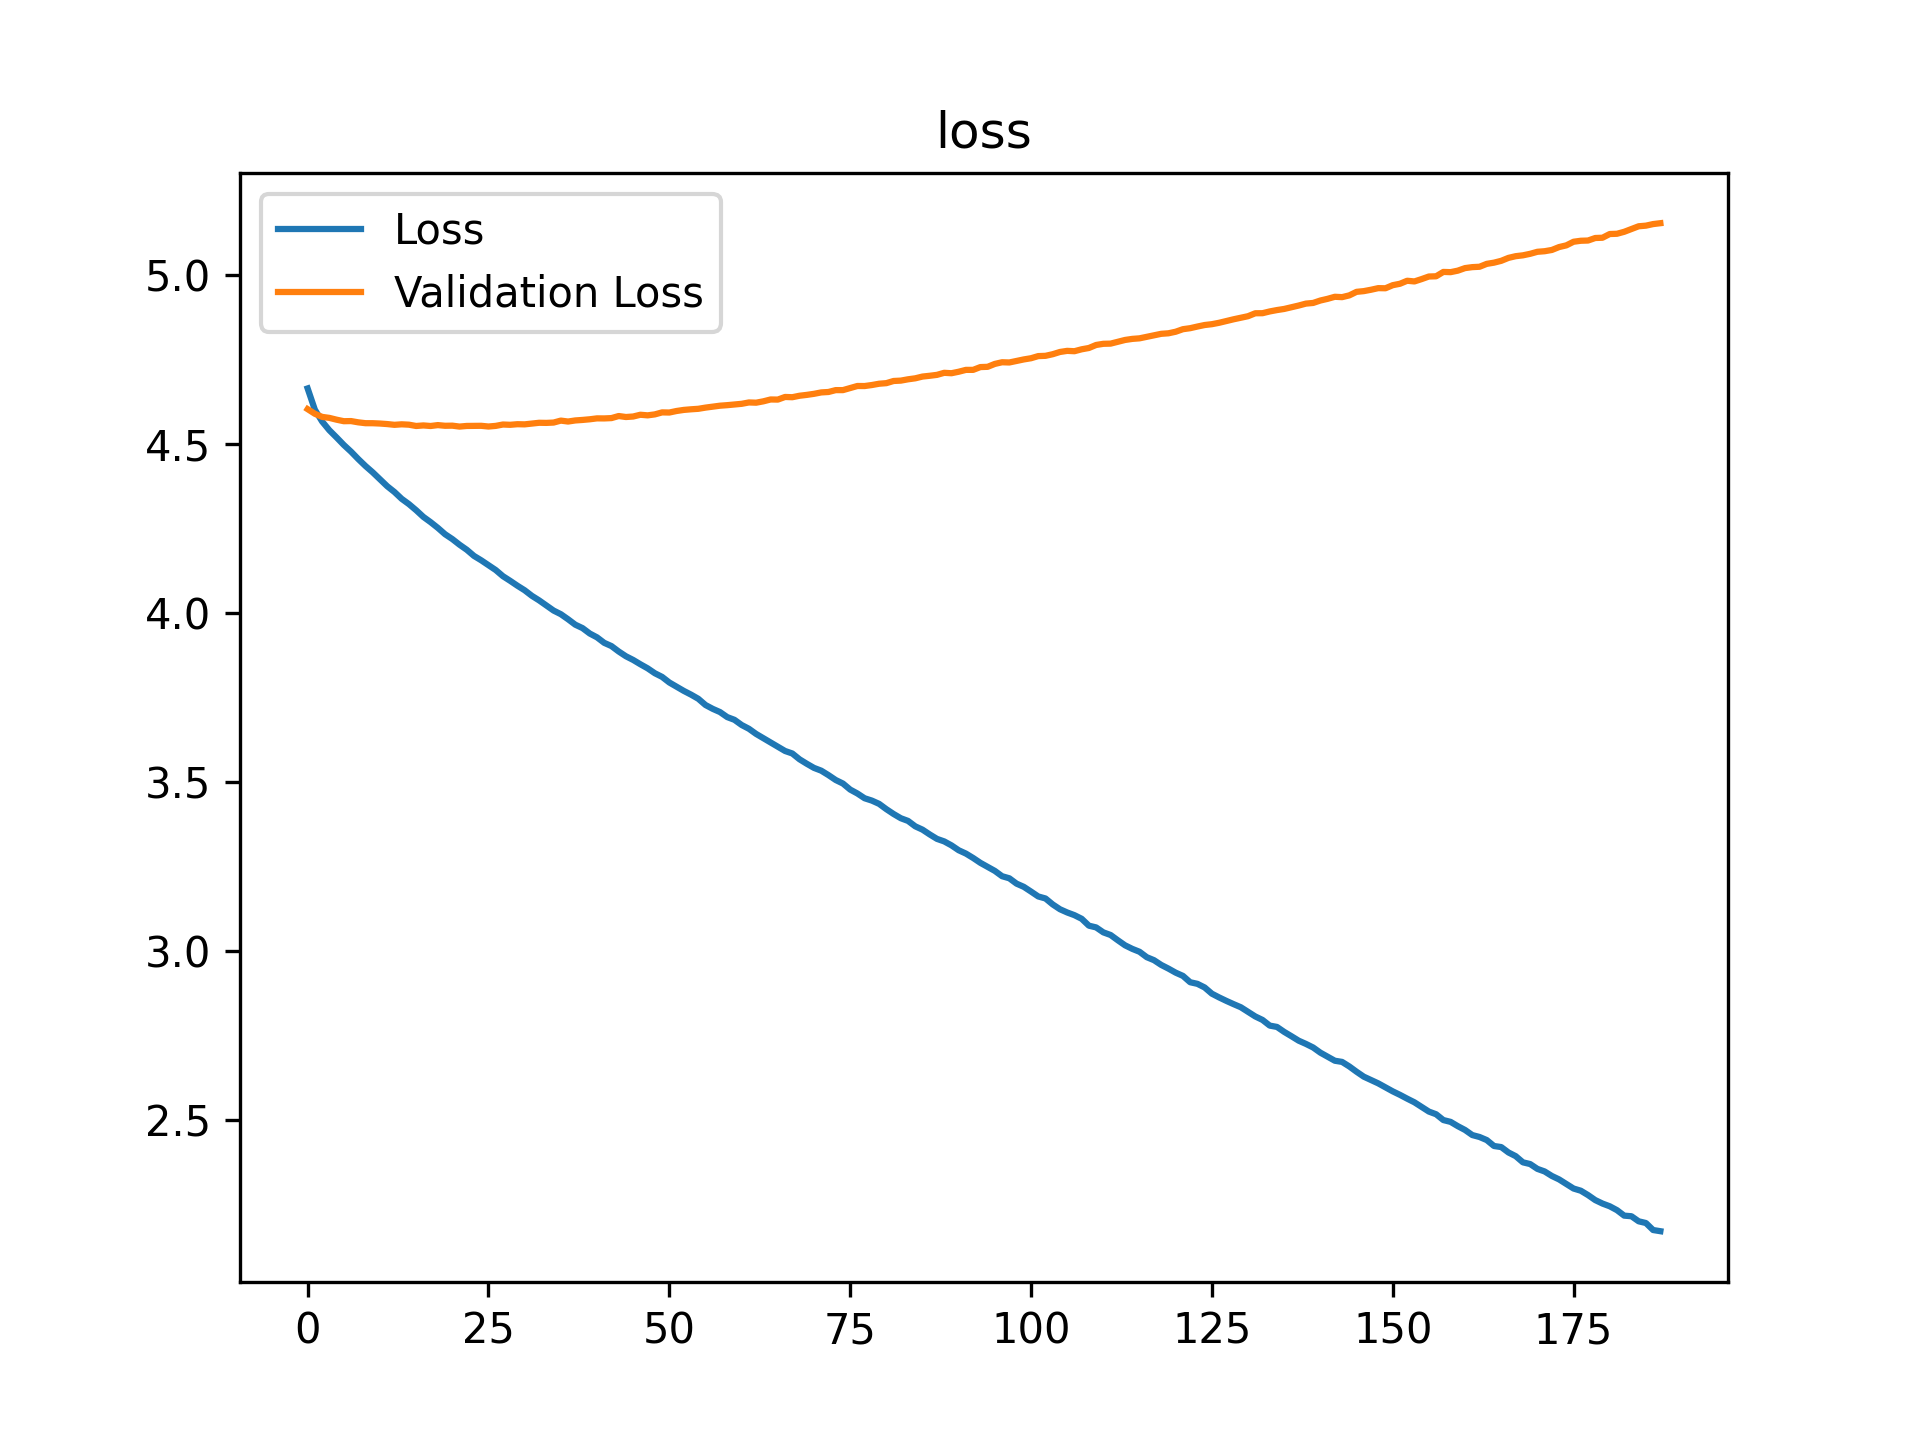
\includegraphics[width=1\linewidth]{recursos/imagens/results/food_wp_loss.png}
         \caption{Aquecimento.}
         \label{results:fig:datasets:4.1}
     \end{subfigure}%
     ~ 
     \begin{subfigure}[t]{0.45\textwidth}
         \centering
         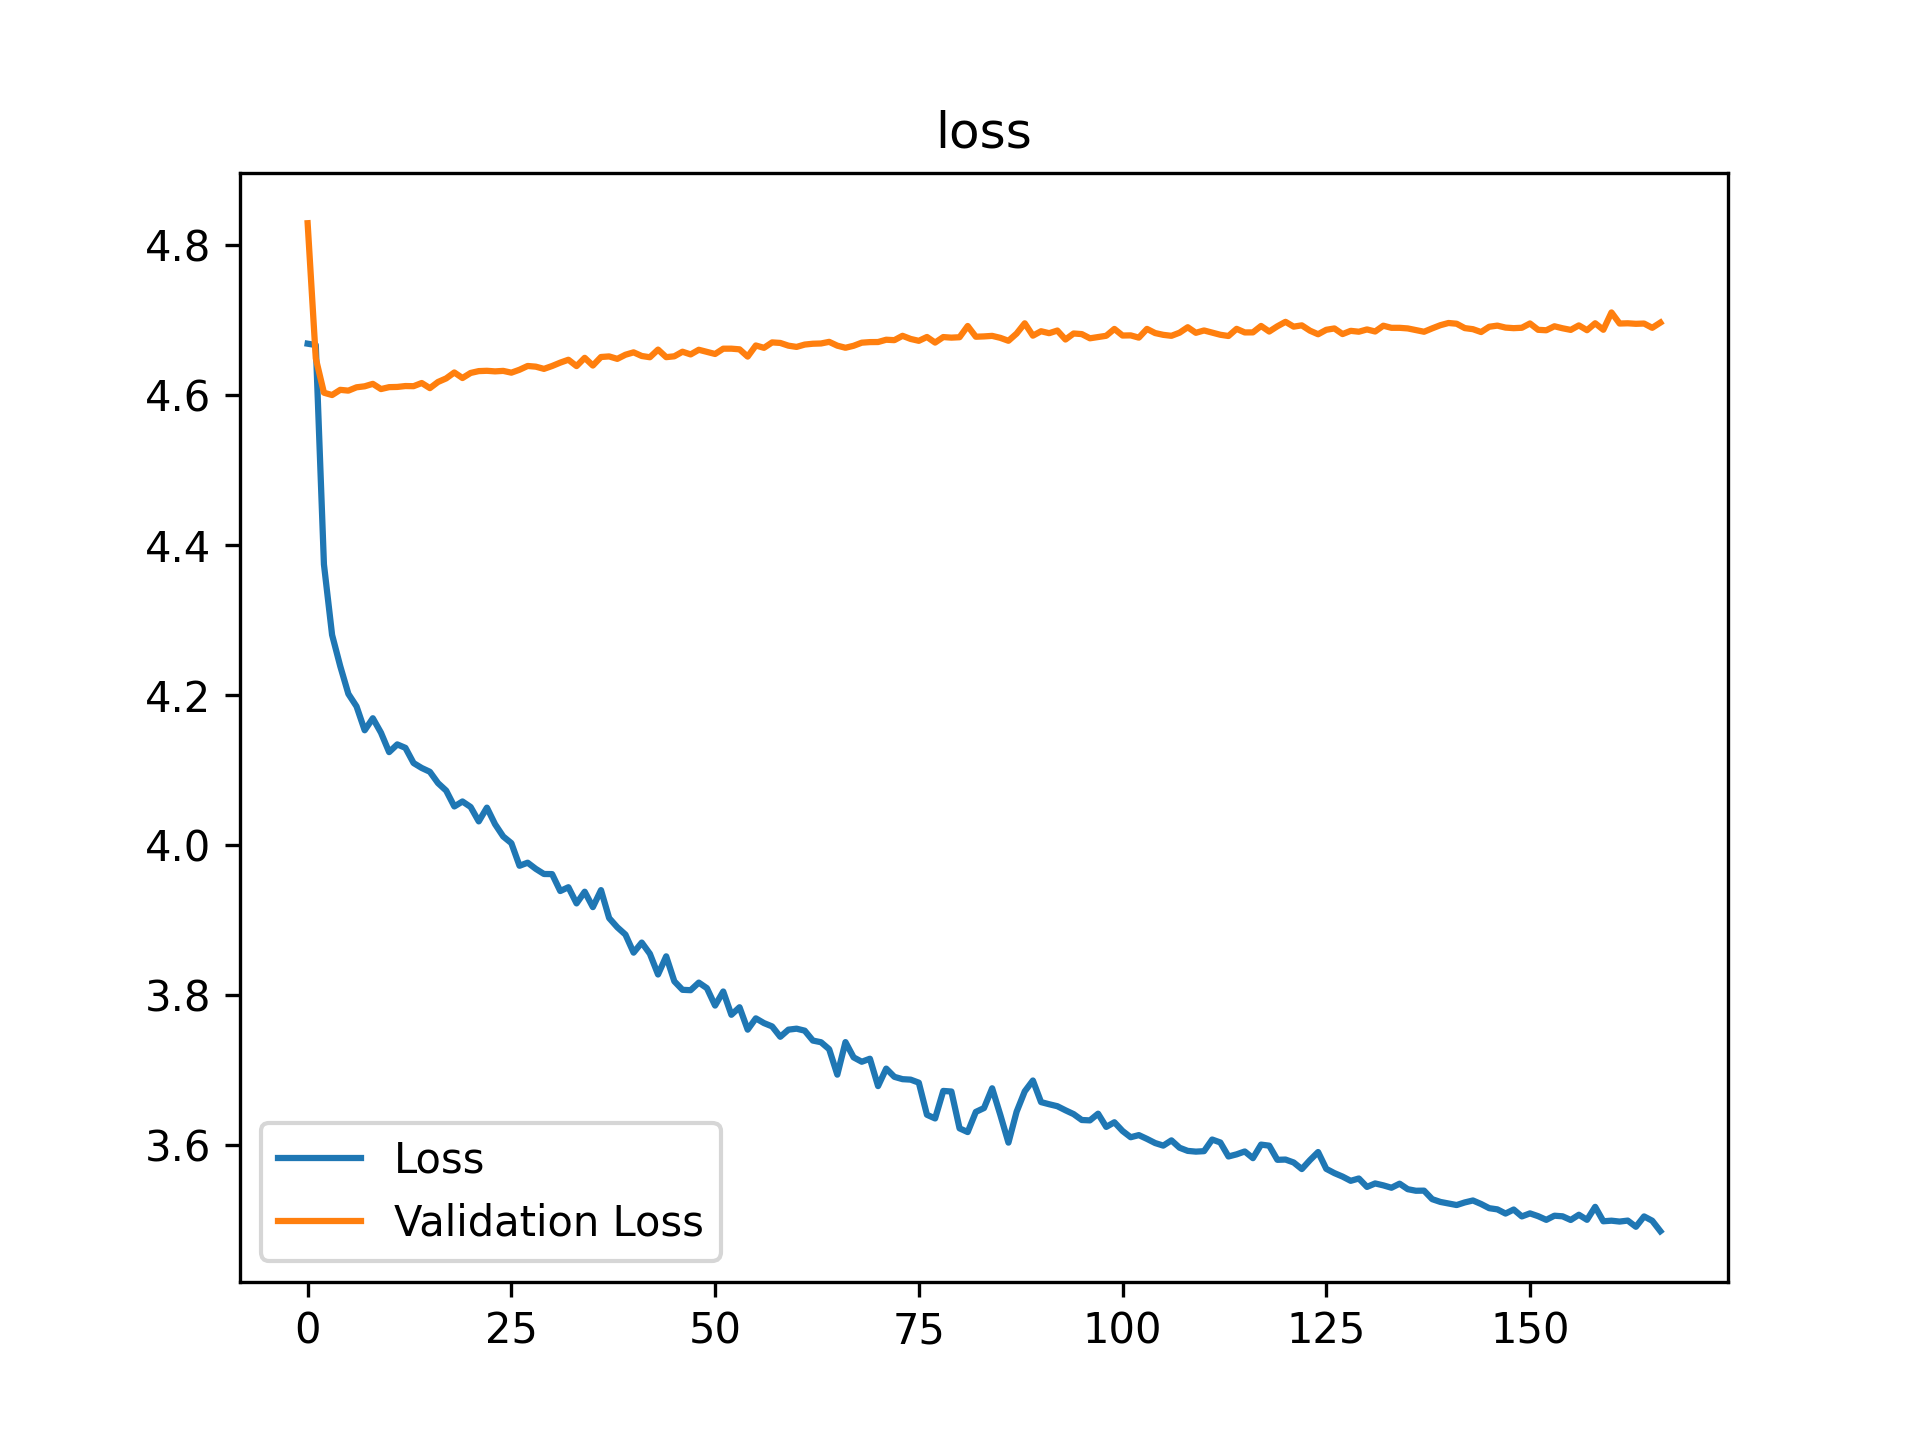
\includegraphics[width=1\linewidth]{recursos/imagens/results/food_loss1.png}
         \caption{Bloco 5.}
         \label{results:fig:datasets:4.2}
     \end{subfigure}%
     ~ 
     
     \begin{subfigure}[t]{0.45\textwidth}
         \centering
         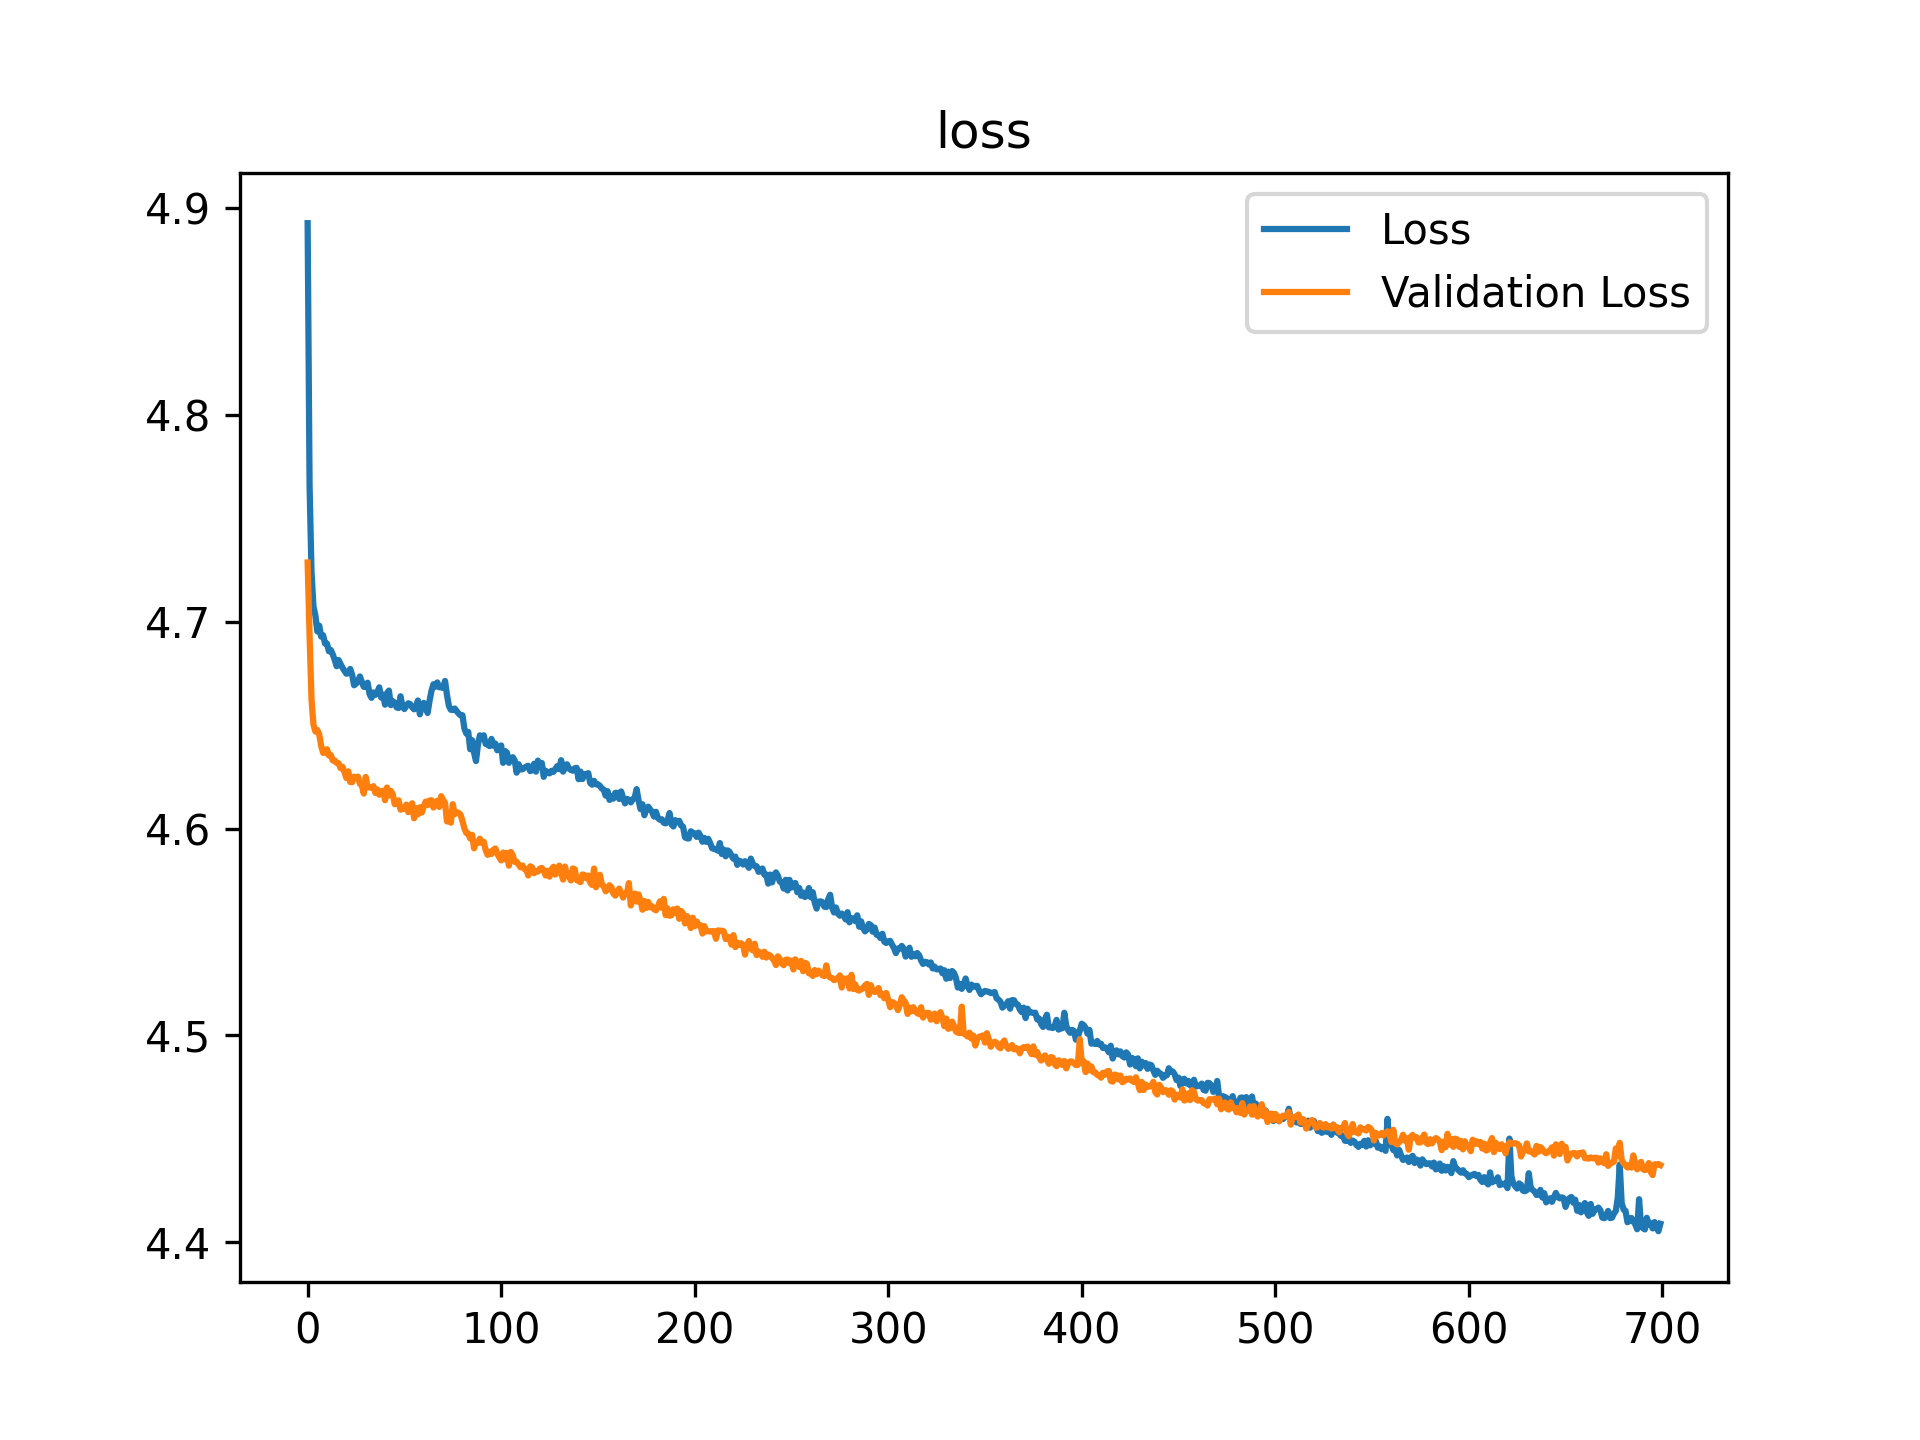
\includegraphics[width=1\linewidth]{recursos/imagens/results/food_loss2.png}
         \caption{Bloco 4.}
         \label{results:fig:datasets:4.3}
     \end{subfigure}
     ~
     \begin{subfigure}[t]{0.45\textwidth}
         \centering
         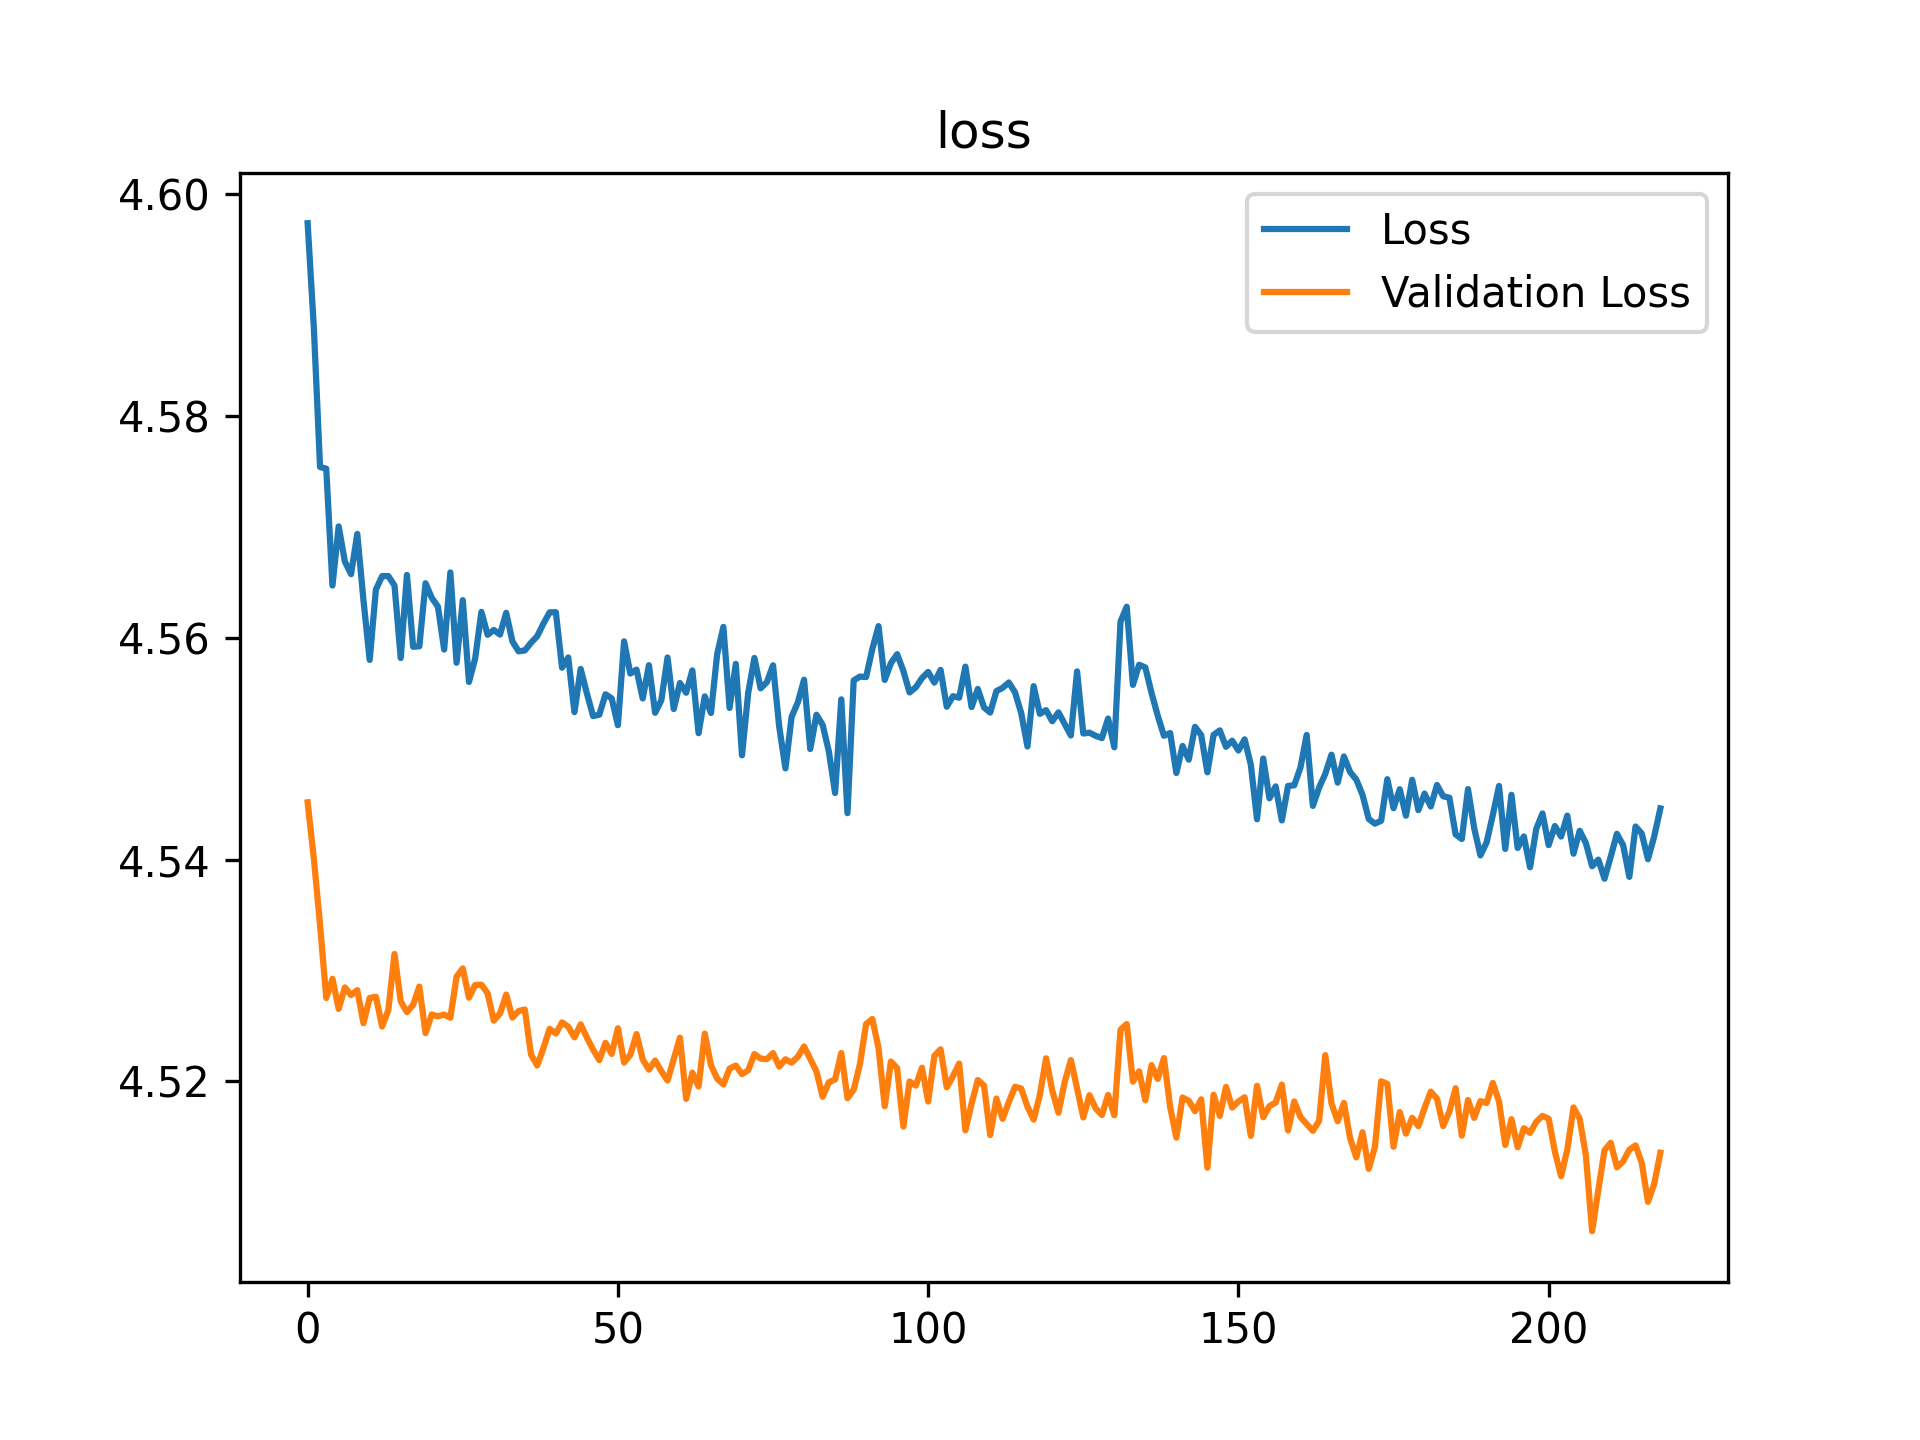
\includegraphics[width=1\linewidth]{recursos/imagens/results/food_loss3.png}
         \caption{Bloco 3.}
         \label{results:fig:datasets:4.4}
     \end{subfigure}
     
     Fonte: do próprio autor.
 \end{figure}

Em suma, a diversidade dos conjuntos de dados utilizados neste estudo forneceu uma avaliação robusta do método BPCAPooling, destacando tanto o seus pontos potenciais quanto a necessidade de otimizações específicas para diferentes cenários. As diferenças nos resultados reforçam a importância da seleção apropriada do conjunto de dados considerando suas características particulares.

\subsubsection{LIME e Preservação de Espacialidade}
\label{results:class:lime}
Em termos de preservação das informações espaciais entre as camadas de \textit{pooling}, o método BPCAPooling se destacou em relação a outros métodos quando analisado em camadas de \textit{pooling} de alto nível em ambos os conjuntos de dados (3ª camada).

No conjunto de dados CIFAR 100, é evidente que as características geométricas das imagens são mantidas ao usar o BPCAPooling. Em contraste com os métodos convencionais, não se observam imagens completamente escurecidas ou com ruído nas camadas de alto nível, como ilustrado na Figura \ref{results:fig:datasets:5} e indicado em destaque em vermelho. Apesar do tamanho menor da imagem no conjunto CIFAR 100, resultando em mapas de características de dimensão $2 \times 2$ nas camadas posteriores, o que torna a preservação espacial um desafio, optou-se por manter a arquitetura VGG-16 original sem alterações estruturais, em vez de remover os blocos convolucionais ulteriores.

\begin{figure}[H]
    \centering
    \caption{Representação com primeira e segunda camada de \textit{pooling} aplicada no conjunto de dados CIFAR 100.}
    \label{results:fig:datasets:5}
    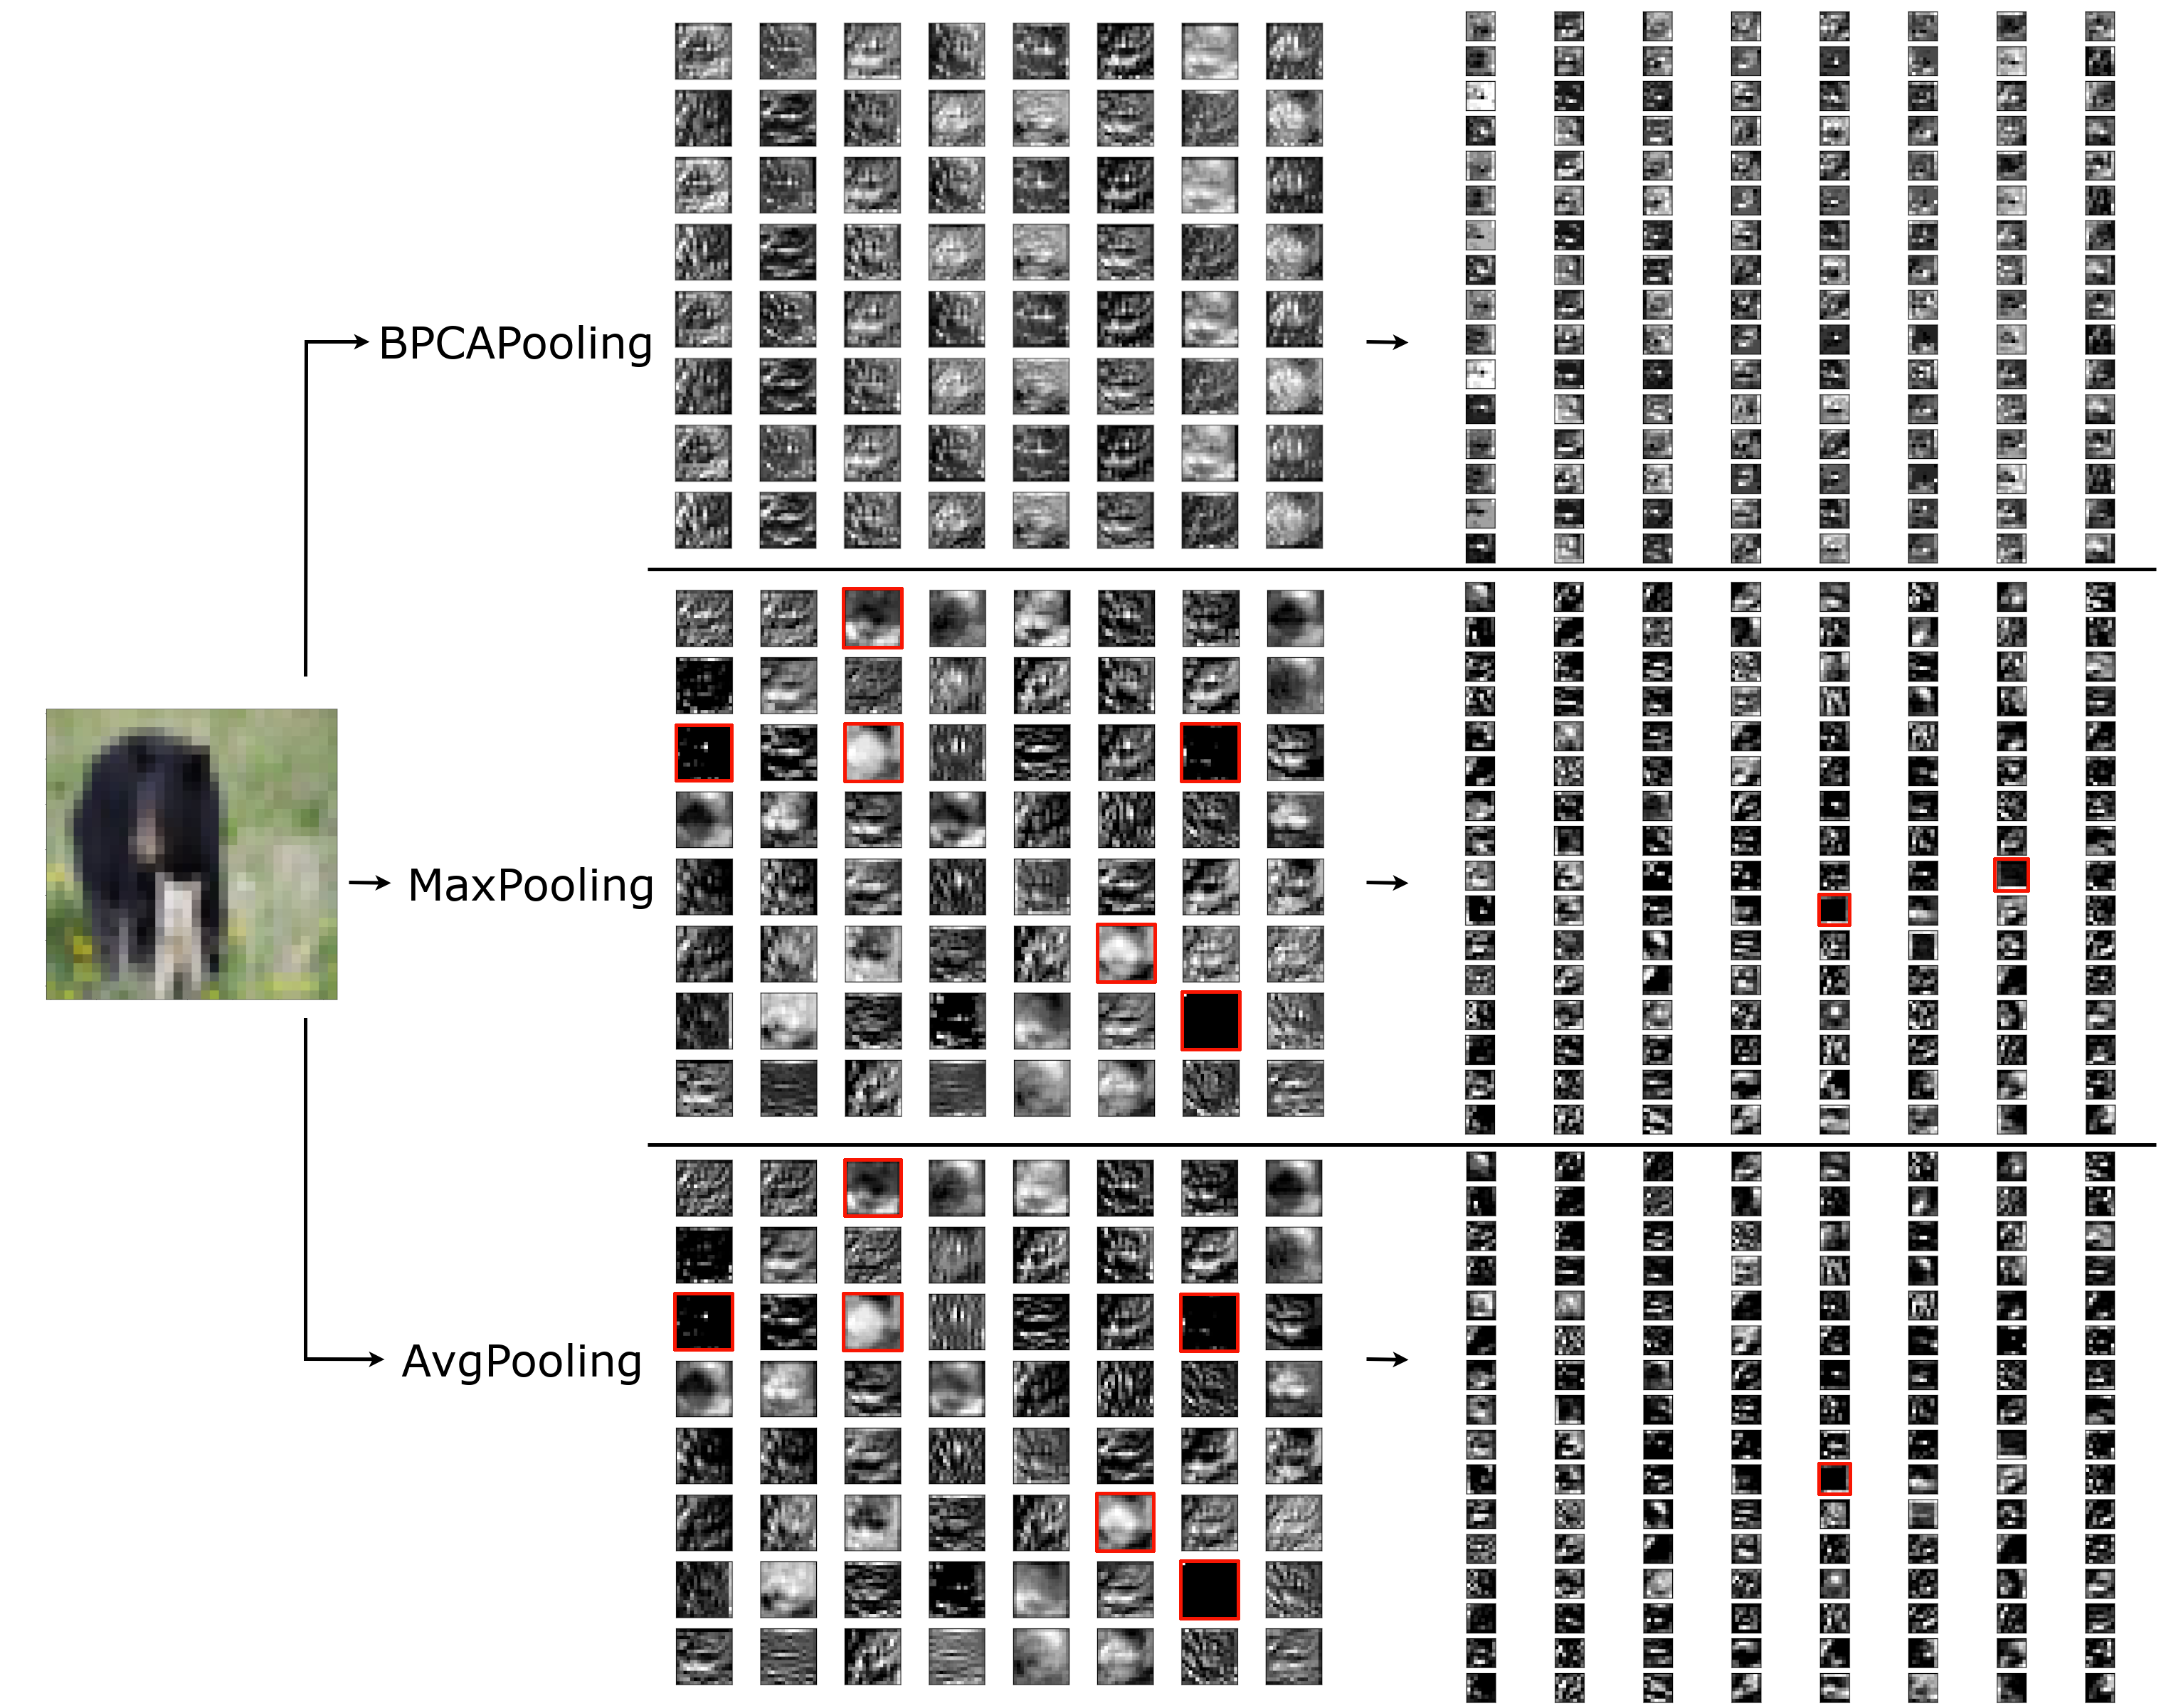
\includegraphics[width=1\textwidth]{recursos/imagens/results/cifar_blocks.png}

    Fonte: do próprio autor.
\end{figure}

Ao analisar as camadas de \textit{pooling} aplicadas ao conjunto de dados \textit{Food}-101, representadas na Figura \ref{results:fig:datasets:6}, observa-se diferenças notáveis nas intensidades das saídas dessas camadas. As saídas resultantes do método \textit{Max Pooling} apresentam menor intensidade, enquanto as saídas do método BPCAPooling exibem maior intensidade, resultando em imagens com maior clareza e definição, principalmente de bordas.

\begin{figure}[H]
   \caption{Resultado visual de camadas de \textit{pooling} do conjunto \textit{Food}-101.}
   \centering
   \label{results:fig:datasets:6}
    \begin{subfigure}[t]{1\textwidth}
        \centering
        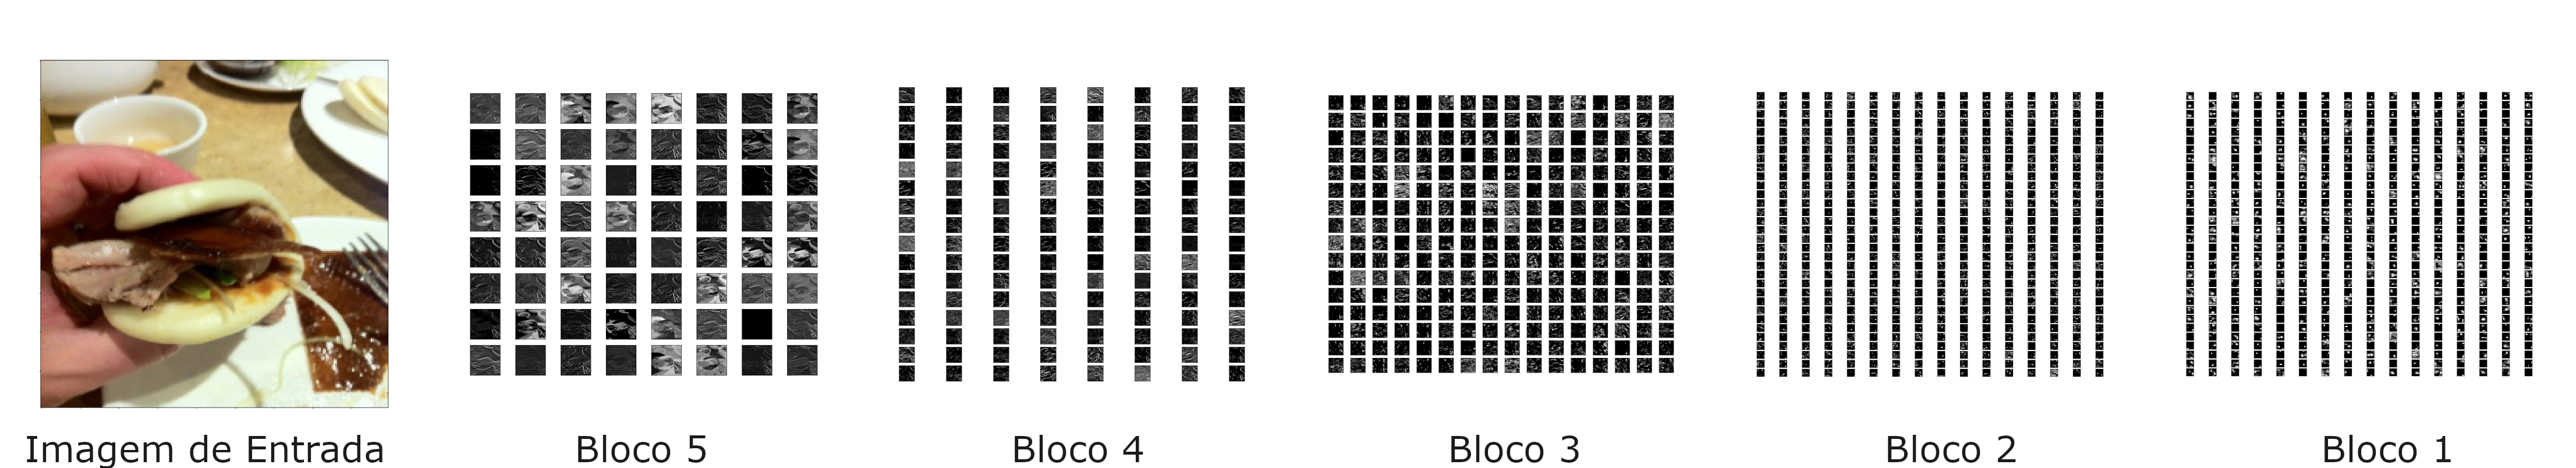
\includegraphics[width=1\linewidth]{recursos/imagens/results/max_by_layer.png}
        \caption{Camadas com \textit{Max Pooling}.}
        \label{results:fig:datasets:6.1}
    \end{subfigure}%
    ~ 

    \begin{subfigure}[t]{1\textwidth}
        \centering
        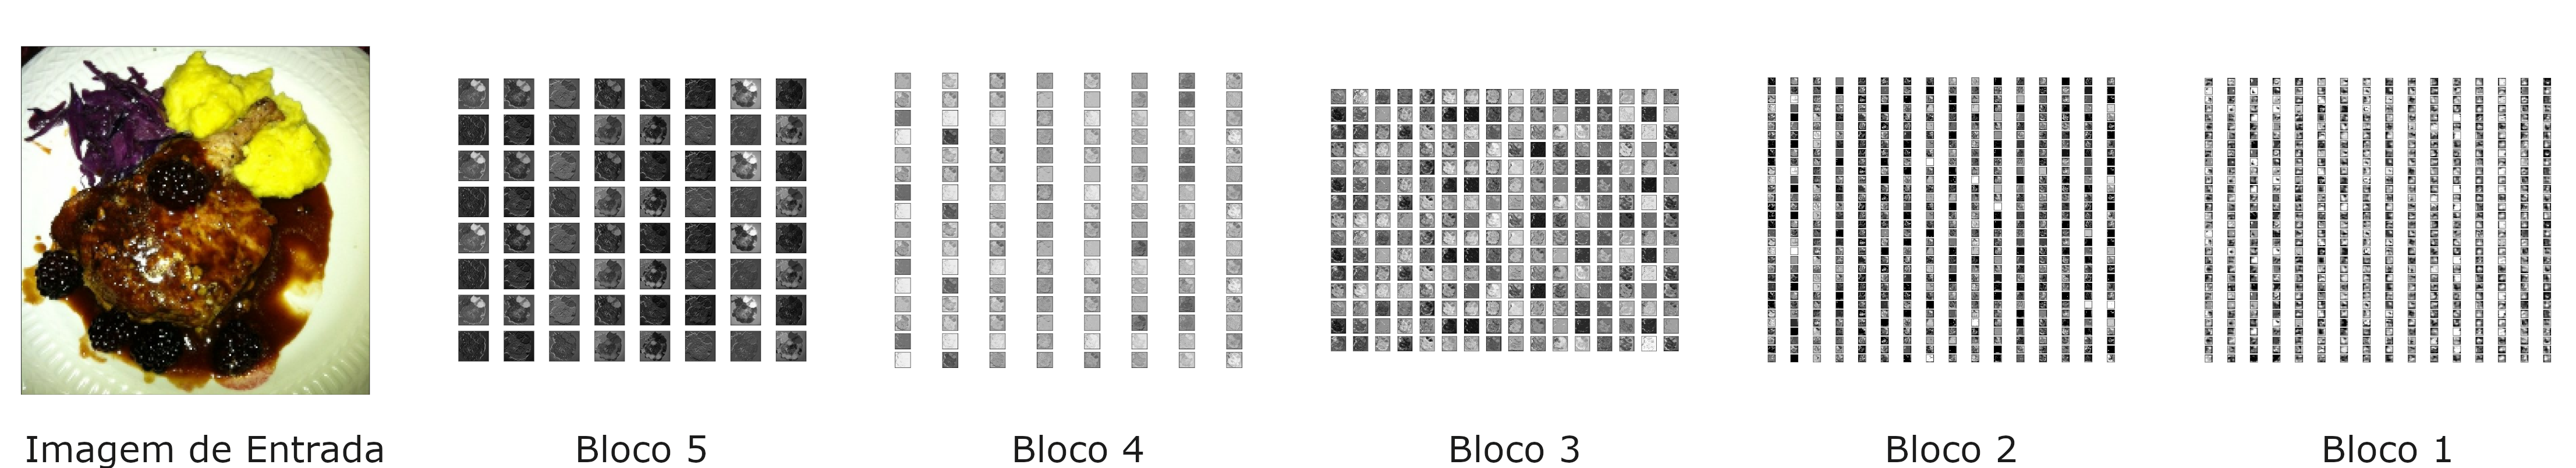
\includegraphics[width=1\linewidth]{recursos/imagens/results/bpca_by_layer.png}
        \caption{Camadas com BPCAPooling.}
        \label{results:fig:datasets:6.2}
    \end{subfigure}%

    Fonte: do próprio autor.
\end{figure}

Outro ponto notável é a discrepância nas últimas camadas de BPCAPooling, como mencionado anteriormente no contexto do conjunto de dados CIFAR 100. As saídas dessas camadas finais de BPCAPooling parecem conter ruídos visuais, enquanto as saídas das últimas camadas com \textit{Max Pooling} aparentam conter mais informações agregadas. Isso é evidenciado na Figura \ref{results:fig:datasets:7}, que mostra resultados com resolução superior a $2 \times 2$, devido à resolução maior das imagens de entrada.

\begin{figure}[H]
    \centering
   \caption{Visualização das últimas camadas de \textit{pooling} no conjunto \textit{Food}-101.}
    \label{results:fig:datasets:7}
    \begin{subfigure}[t]{0.5\textwidth}
        \centering
        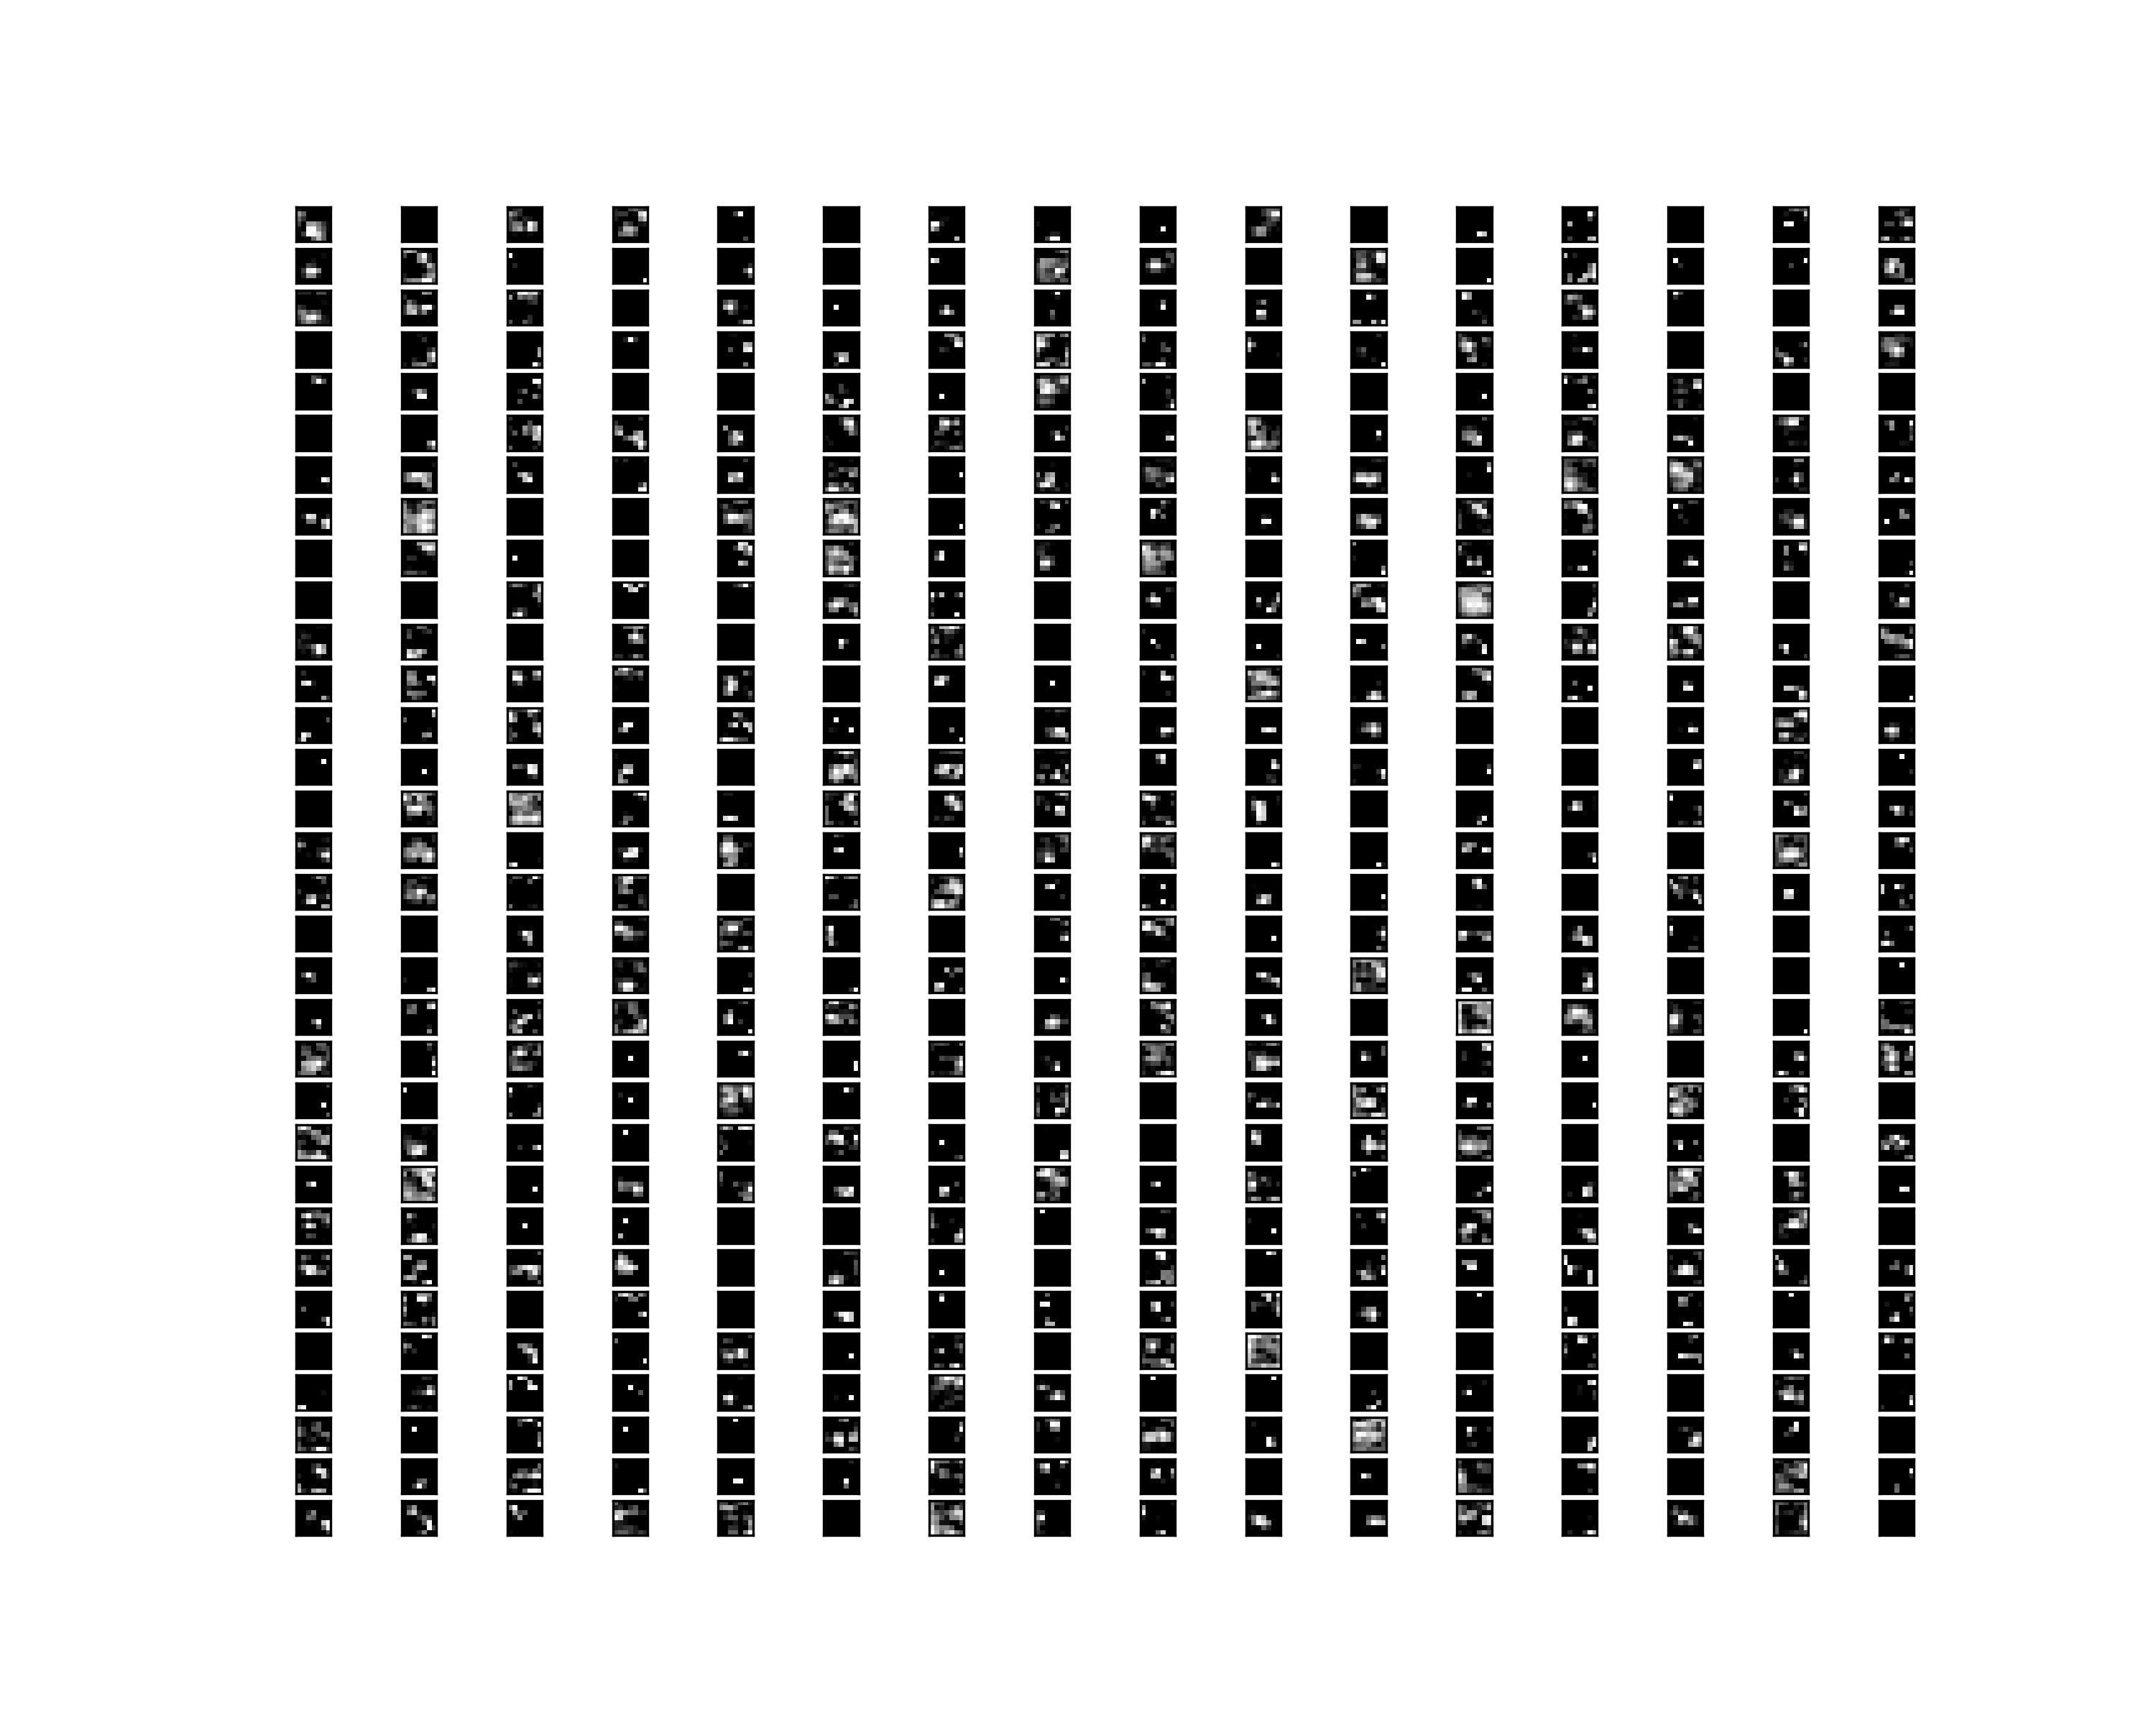
\includegraphics[width=1\linewidth]{recursos/imagens/results/block5_pool_4_max.png}
        \caption{Camada com \textit{Max Pooling}.}
        \label{results:fig:datasets:7.1}
    \end{subfigure}%
    ~
    \begin{subfigure}[t]{0.5\textwidth}
        \centering
        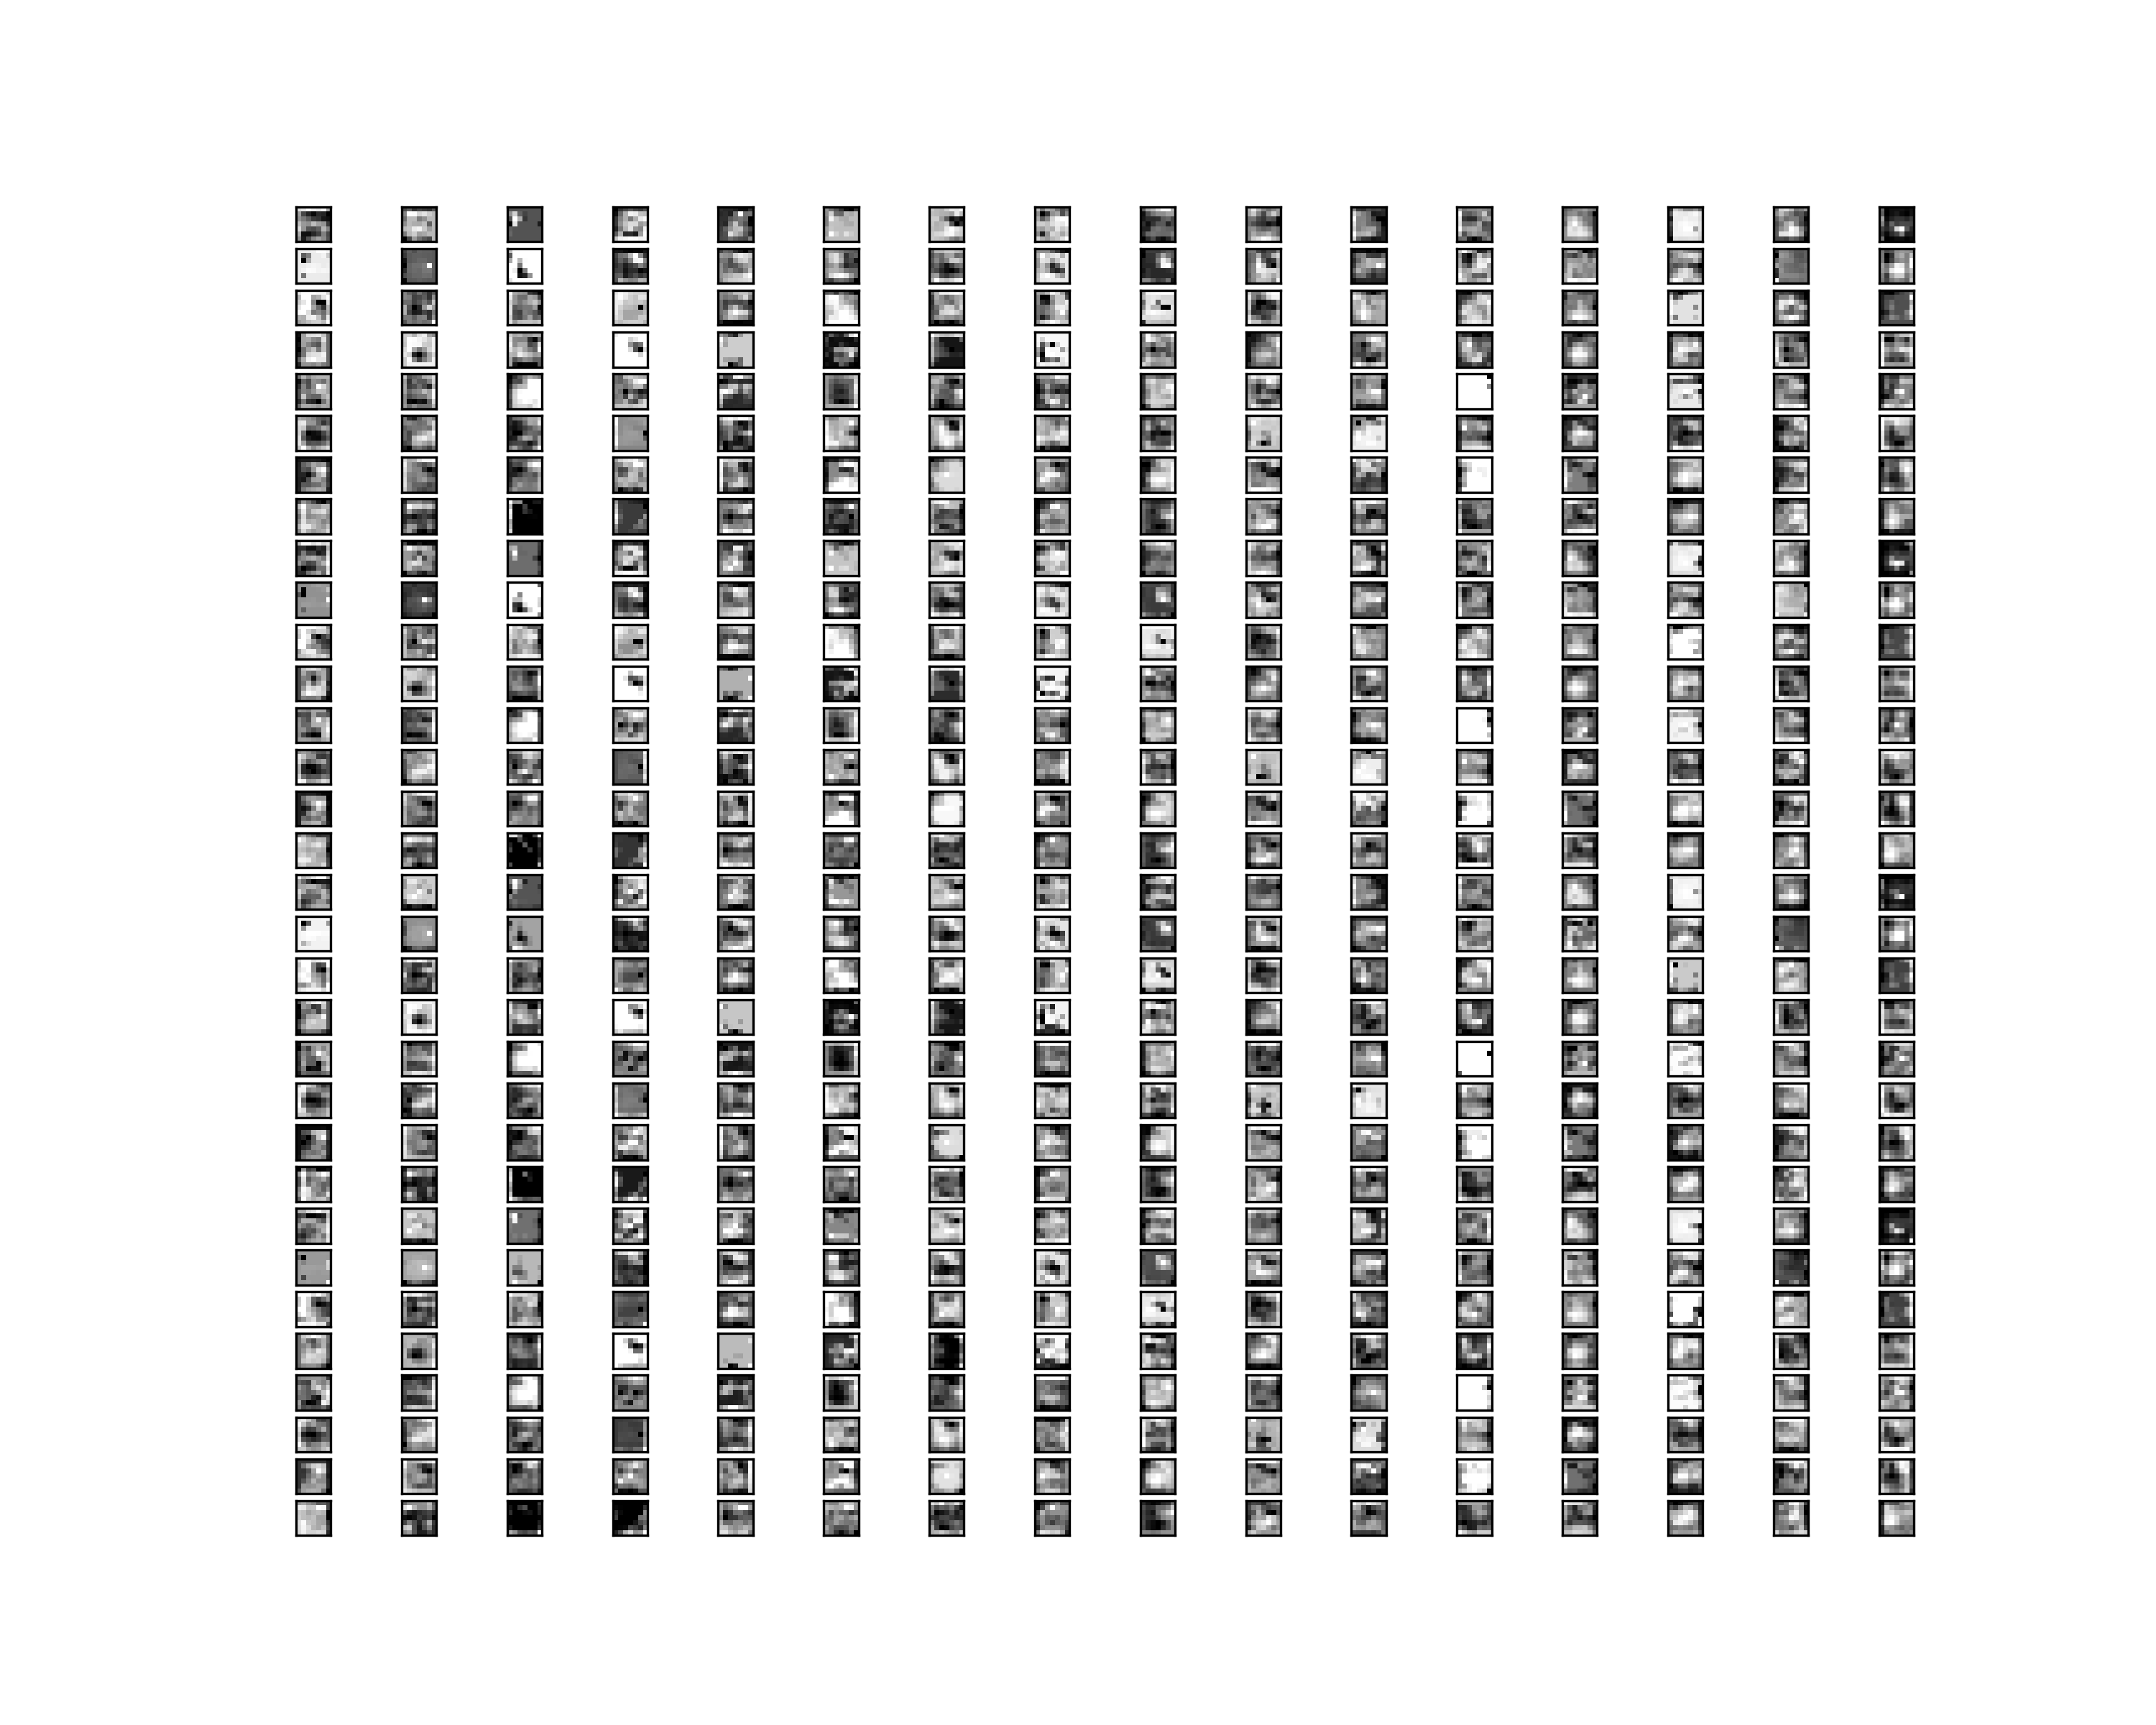
\includegraphics[width=1\linewidth]{recursos/imagens/results/block5_pool_4_bpca.png}
        \caption{Camada com BPCAPooling.}
        \label{results:fig:datasets:7.2}
    \end{subfigure}%

    Fonte: do próprio autor.
\end{figure}

No contexto das análises realizadas com LIME, é importante ressaltar um fator crucial para o desempenho dessa técnica: o tamanho da amostra de imagem. Ao considerar as imagens do conjunto de dados CIFAR 100, obter resultados satisfatórios foi desafiador devido ao pequeno tamanho de $32 \times 32$ pixels de cada exemplo do conjunto de dados. Nessa escala, cada pixel possui um peso significativo em comparação com a área total da imagem. Na Figura \ref{results:fig:datasets:8}, as contribuições positivas são representadas por pixels verdes e as contribuições negativas por pixels vermelhos para uma inferência de classe específica. Entretanto, como evidenciado na Figura, todos os pixels influenciam positiva ou negativamente a classificação devido ao pequeno tamanho da imagem, não havendo distinções por região.

\begin{figure}[H]
    \centering
    \caption{Exemplo de imagens explicadas por LIME no conjunto de dados CIFAR 100.}
    \label{results:fig:datasets:8}
    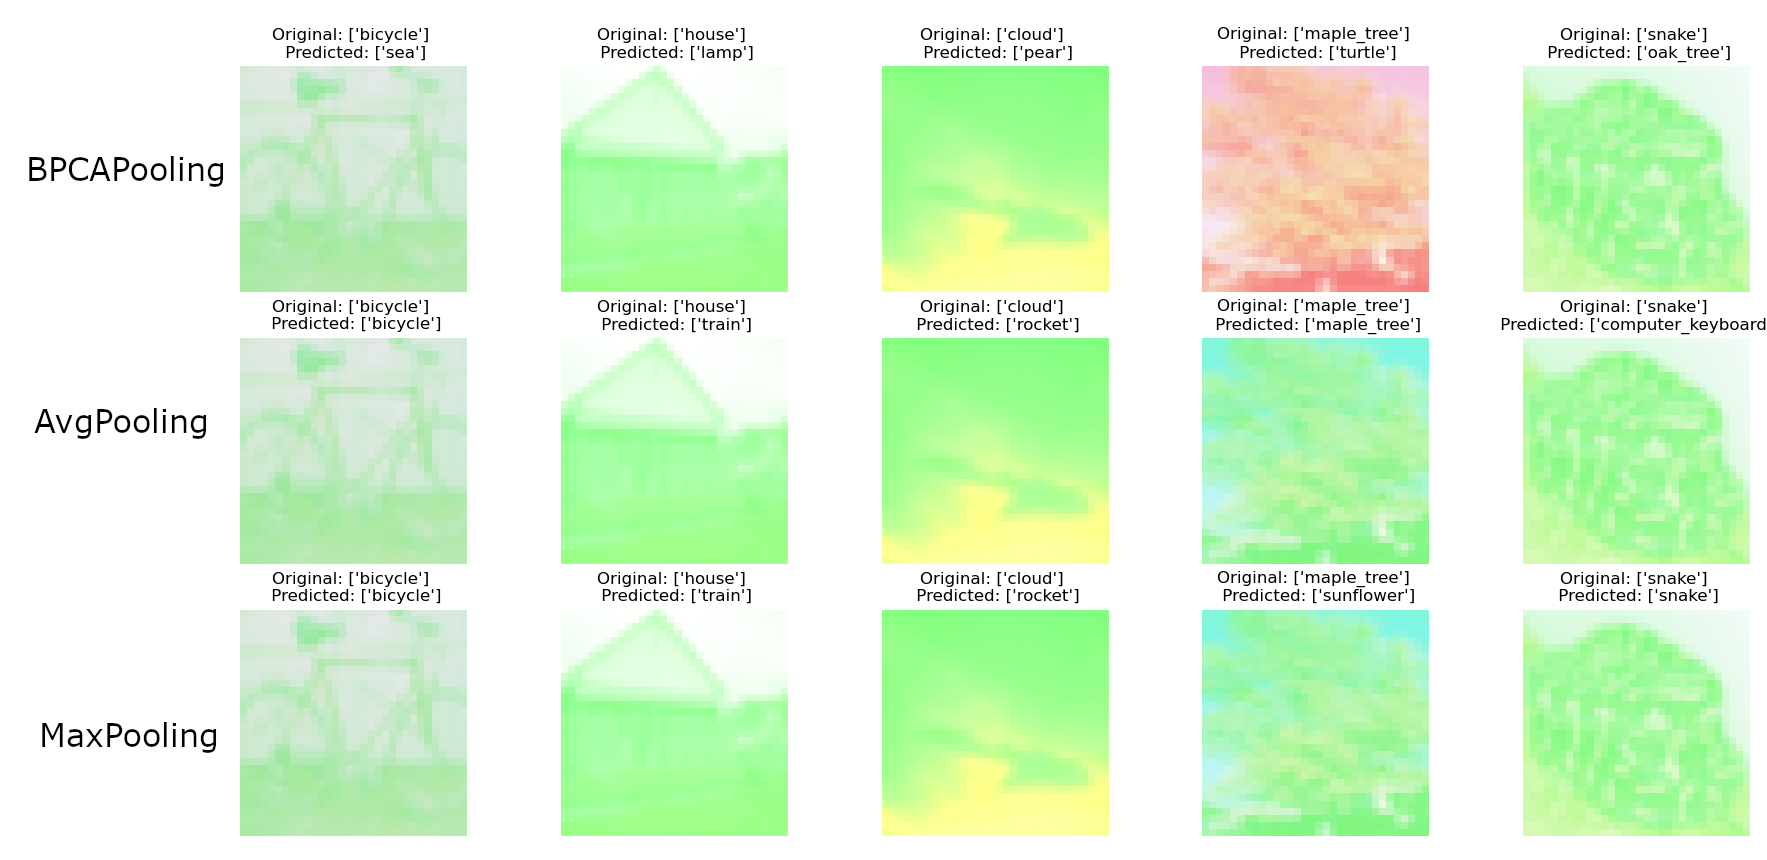
\includegraphics[width=1\textwidth]{recursos/imagens/results/lime_explanations_cifar.png}

    Fonte: do próprio autor.
\end{figure}

Por outro lado, ao examinar as imagens relacionadas ao conjunto de dados \textit{Food}-101, é evidente que o LIME oferece mais \textit{insights} sobre as classificações realizadas. Como demonstrado na Figura \ref{results:fig:datasets:9}, apenas as regiões relevantes (positivamente ou negativamente) são destacadas, apresentando um tamanho de imagem apropriado, ao contrário do conjunto de dados CIFAR 100. Além disso, a análise dos resultados revela que, em alguns casos, a rede enfoca mais em embalagens, utensílios e louças, diminuindo a relevância das informações relacionadas à alimentação. Esta questão poderia ser abordada ao melhorar a estratégia de aquisição de dados, como ampliar as imagens ou aplicar técnicas de segmentação (por exemplo, \cite{rother2004grabcut}), garantindo que a comida ocupe a maior parte da área da imagem.

\begin{figure}[H]
    \centering
    \caption{Exemplo de imagens explicadas por LIME no conjunto de dados \textit{Food}-100.}
    \label{results:fig:datasets:9}
    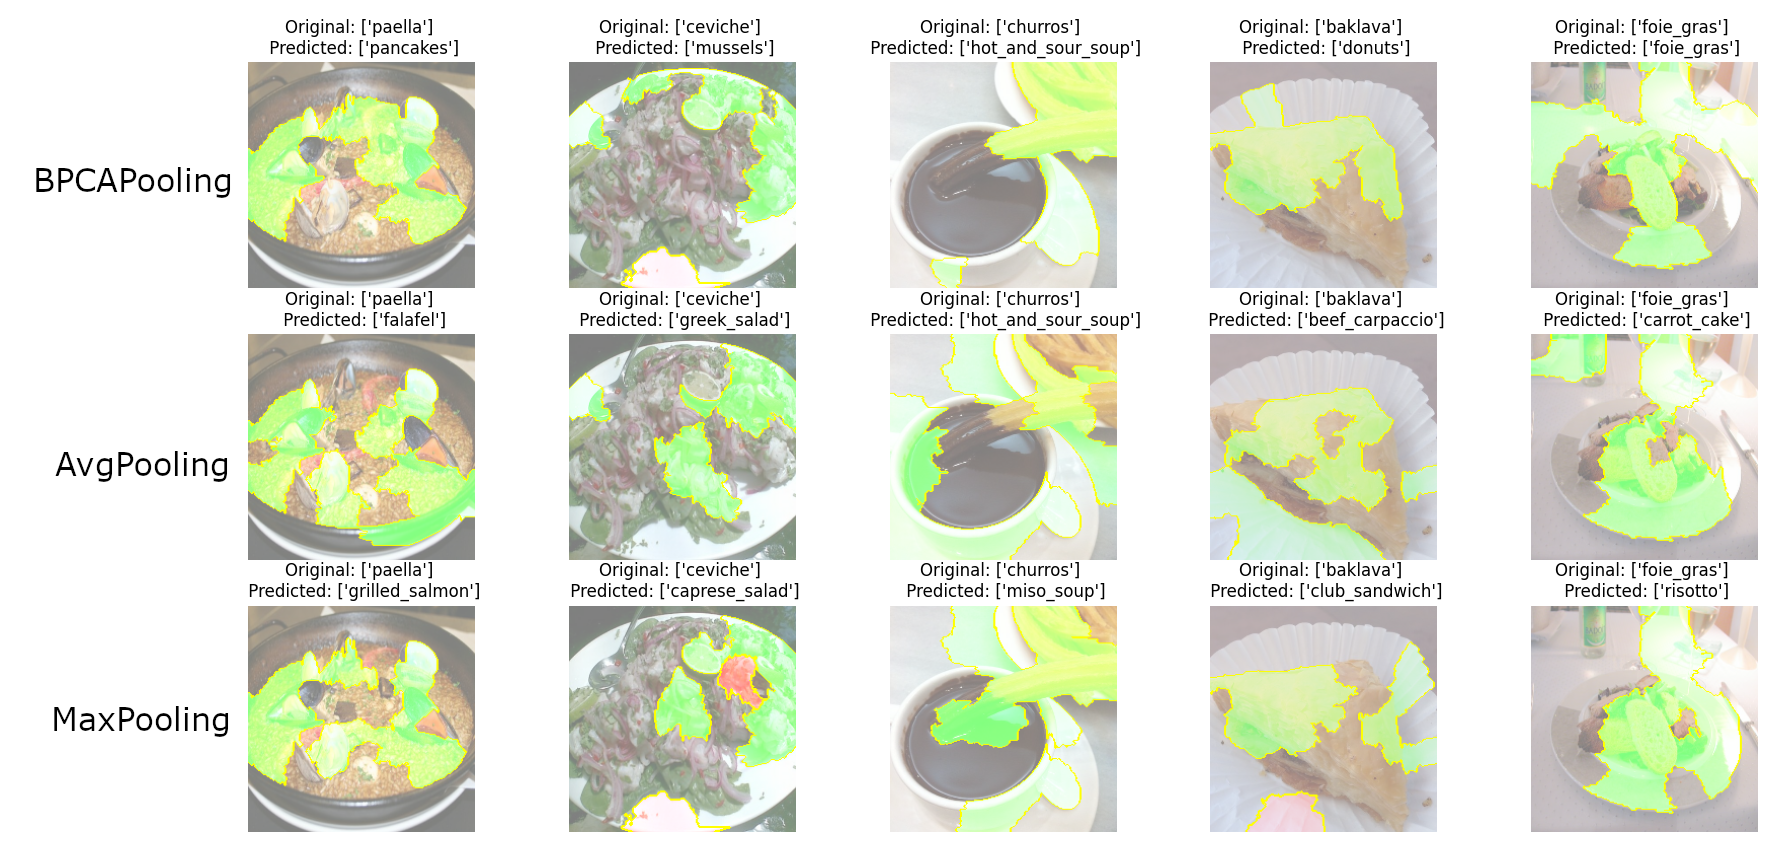
\includegraphics[width=1\textwidth]{recursos/imagens/results/lime_explanations_food.png}

    Fonte: do próprio autor.
\end{figure}


\subsubsection{Trabalhos Futuros}
\label{results:class:future}
Como mencionado na Seção \ref{project:transf}, os experimentos de classificação empregaram os princípios de transferência de aprendizado, o que comumente oferece vantagens devido ao reaproveitamento de pesos de arquiteturas treinadas em grandes conjuntos de dados \citep{Pan2010}. No entanto, embora as camadas de \textit{pooling} não tenham parâmetros treináveis diretamente afetados pela retro-propagação, elas influenciam diretamente as camadas de convolução subsequentes. Isso levanta a questão: \quotes{Será que o uso de transferência de aprendizado realmente contribuiu para a aplicação do método BPCAPooling nos experimentos realizados?} Uma vez que as camadas da rede passam a ficar com os pesos aquecidos, mas com o viés da utilização de um redutor de dimensionalidade que não mantém espacialidade, como é o caso do \textit{Max Pooling} e \textit{Avg Pooling}.

Além disso, outra questão pendente diz respeito a quais camadas precisam ser descongeladas para obter os melhores resultados possíveis com o método, já que investir em camadas associadas aos conceitos de espacialidade parece ser uma estratégia promissora, como comentado na Seção \ref{results:class:datasets}, que demonstra maior progresso no quarto bloco convolucional.

Por fim, a complexidade do método proposto é uma limitação. Um teste realizado com a arquitetura EfficientNetB0 \citep{Tan2019Efficientnet:Networks}, que possui $17$ camadas de \textit{pooling}, substituindo os métodos convencionais por BPCAPooling resultou em um tempo estimado de treinamento da fase de aquecimento de aproximadamente \textit{2.100} horas, de acordo com os padrões de desempenho comentados na Seção \ref{results:class}.

Para futuros trabalhos que visam aplicar o método BPCAPooling como camada de \textit{pooling} para arquiteturas de classificação, sugere-se a não utilização de transferência de aprendizado para o método, mas sim a realização de fases de treinamento e validação mais extensas, além do uso de conjuntos de dados equivalentes ao ImageNet, o que é um desafio devido às necessidades de \textit{hardware} que surgiriam. Uma sugestão adicional seria propor alternativas para otimizar a complexidade do código associado ao método BPCAPooling. Por fim, uma terceira ideia para trabalhos futuros, que também exigiria considerações sobre o \textit{hardware} necessário para os experimentos, seria a aplicação de mais épocas no descongelamento de determinados blocos convolucionais durante o processo de \textit{fine-tuning}, visando permitir a exploração mais profunda dos mapas de características e potencializar os aspectos de preservação espacial.


\subsection{Resultados da Segmentação Semântica}
\label{results:semantic}
Em relação aos resultados da segmentação semântica, é relevante destacar que as discussões e descobertas abordadas na tarefa de classificação (Seção \ref{results:class}) foram consideradas como um primeiro passo rumo à implementação do método BPCA como camada de \textit{pooling} (BPCAPooling) na tarefa subsequente de segmentação semântica. Esta transição para uma nova tarefa demandaria validações finais para aprimorar o processo experimental específico para esse contexto.

É importante observar que, ao considerar as segmentações realizadas, os resultados obtidos com a aplicação do método BPCAPooling apresentaram similaridades em termos de valores quando comparados ao método tradicional \textit{Max Pooling} na arquitetura da U-Net. Essa comparação pode ser visualizada nas Tabelas \ref{results:semantic:tab:1} e \ref{results:semantic:tab:2}.

\begin{table}[H]
    \centering
    \caption{Resultados de U-Nets treinadas por 500 épocas no conjunto de dados \textit{Oxford-IIIT Pets} com base em acurácia.}
    \label{results:semantic:tab:1}
    \resizebox{1\textwidth}{!}{
        \begin{tabular}{l|l|l|l|l|l}
            \multicolumn{1}{c|}{\textbf{Método de \textit{Pooling}}} & \multicolumn{1}{c|}{\textbf{Tempo de Execução}}  & \multicolumn{2}{c|}{\textbf{Acurácia (\%)}}                                    & \multicolumn{2}{c}{\textbf{\textit{Loss}}}                                    \\
            \cline{3-6}
            \multicolumn{1}{c|}{}                                    & \multicolumn{1}{c|}{\textbf{(minutos)}}          & \multicolumn{1}{c|}{\textbf{Treino}} & \multicolumn{1}{c|}{\textbf{Validação}} & \multicolumn{1}{c|}{\textbf{Treino}} & \multicolumn{1}{c}{\textbf{Validação}} \\
            \hline
            BPCAPooling                                              &  252:82                                         &  87,982                               &  87,50                                  &  \textbf{0,5160}                     &  \textbf{0,7284}                        \\
            \textit{Max Pooling}                                     &  \textbf{96:98}                                 &  \textbf{89,381}                      &  \textbf{88,64}                         &  0,5484                              &  0,8109                                 \\
        \end{tabular}
    }

    \vspace*{1 cm}
    Fonte: do próprio autor.
\end{table}

\begin{table}[H]
    \centering
    \caption{Resultados de U-Nets treinadas por 500 épocas no conjunto de dados \textit{Oxford-IIIT Pets} com base em mIoU.}
    \label{results:semantic:tab:2}
    \resizebox{1\textwidth}{!}{
        \begin{tabular}{l|l|l|l|l|l|l|l|l|l}
            \multicolumn{1}{c|}{\textbf{Método de \textit{Pooling}}} & \multicolumn{1}{c|}{\textbf{Tempo de Execução}}  & \multicolumn{2}{c|}{\textbf{Acurácia (\%)}}                                    & \multicolumn{2}{c|}{\textbf{\textit{Loss}}}                                    & \multicolumn{2}{c|}{\textbf{mIoU}}                                             & \multicolumn{2}{c}{\textbf{Dice}}                                              \\
            \cline{3-10}
            \multicolumn{1}{c|}{}                                    & \multicolumn{1}{c|}{\textbf{(minutos)}}          & \multicolumn{1}{c|}{\textbf{Treino}} & \multicolumn{1}{c|}{\textbf{Validação}} & \multicolumn{1}{c|}{\textbf{Treino}} & \multicolumn{1}{c|}{\textbf{Validação}}  & \multicolumn{1}{c|}{\textbf{Treino}} & \multicolumn{1}{c|}{\textbf{Validação}} & \multicolumn{1}{c|}{\textbf{Treino}} & \multicolumn{1}{c}{\textbf{Validação}}  \\
            \hline
            BPCAPooling                                              &  154:09                                          &  86,30                               &  86,77                                  &  0,5756                              &  \textbf{0,6659}                        & 0,3344                               & 0,3333                                  & \textbf{0,8892}                       & 0,8953                                  \\
            \textit{Max Pooling}                                     &  \textbf{57:23}                                  &  \textbf{88,750}                     &  \textbf{88,61}                         &  \textbf{0,4683}                     &  0,6668                                 & \textbf{0,3367}                      & \textbf{0,3367}                         & 0,8887                               & 0,8953                                   \\
        \end{tabular}
    }

    \vspace*{1 cm}
    Fonte: do próprio autor.
\end{table}

Analisando as tabelas anteriores, observa-se que, embora as métricas adotadas para conduzir os experimentos sejam acurácia e mIoU, a \textit{loss} associada ao BPCAPooling foi menor nas etapas de validação, conforme evidenciado na Figuras \ref{results:fig:semantic:metrics1.2} e \ref{results:fig:semantic:metrics1.4}. Além disso, a métrica Dice demonstrou ser igual ou superior aos resultados obtidos com o uso do BPCAPooling. Entretanto, é importante ressaltar que, quantitativamente, a métrica mIoU tende a penalizar mais instâncias únicas com classificações ruins do que a métrica Dice, mesmo quando ambas concordam que essa instância é ruim. Ademais, a métrica mIoU tende a agravar os erros, resultando em um efeito de \quotes{quadratura} em relação ao Dice. Como resultado, a métrica Dice parece medir algo mais próximo do desempenho médio, como evidenciado nas Figuras \ref{results:fig:semantic:metrics2.3} e \ref{results:fig:semantic:metrics3.3}, enquanto a mIoU mede algo mais próximo do pior caso de desempenho.

\begin{figure}[H]
    \centering
    \caption{Métricas de U-Nets com 500 épocas no conjunto de dados \textit{Oxford-IIIT Pets} baseada em acurácia.}
    \label{results:fig:semantic:metrics1}
     \begin{subfigure}[t]{0.45\textwidth}
         \centering
         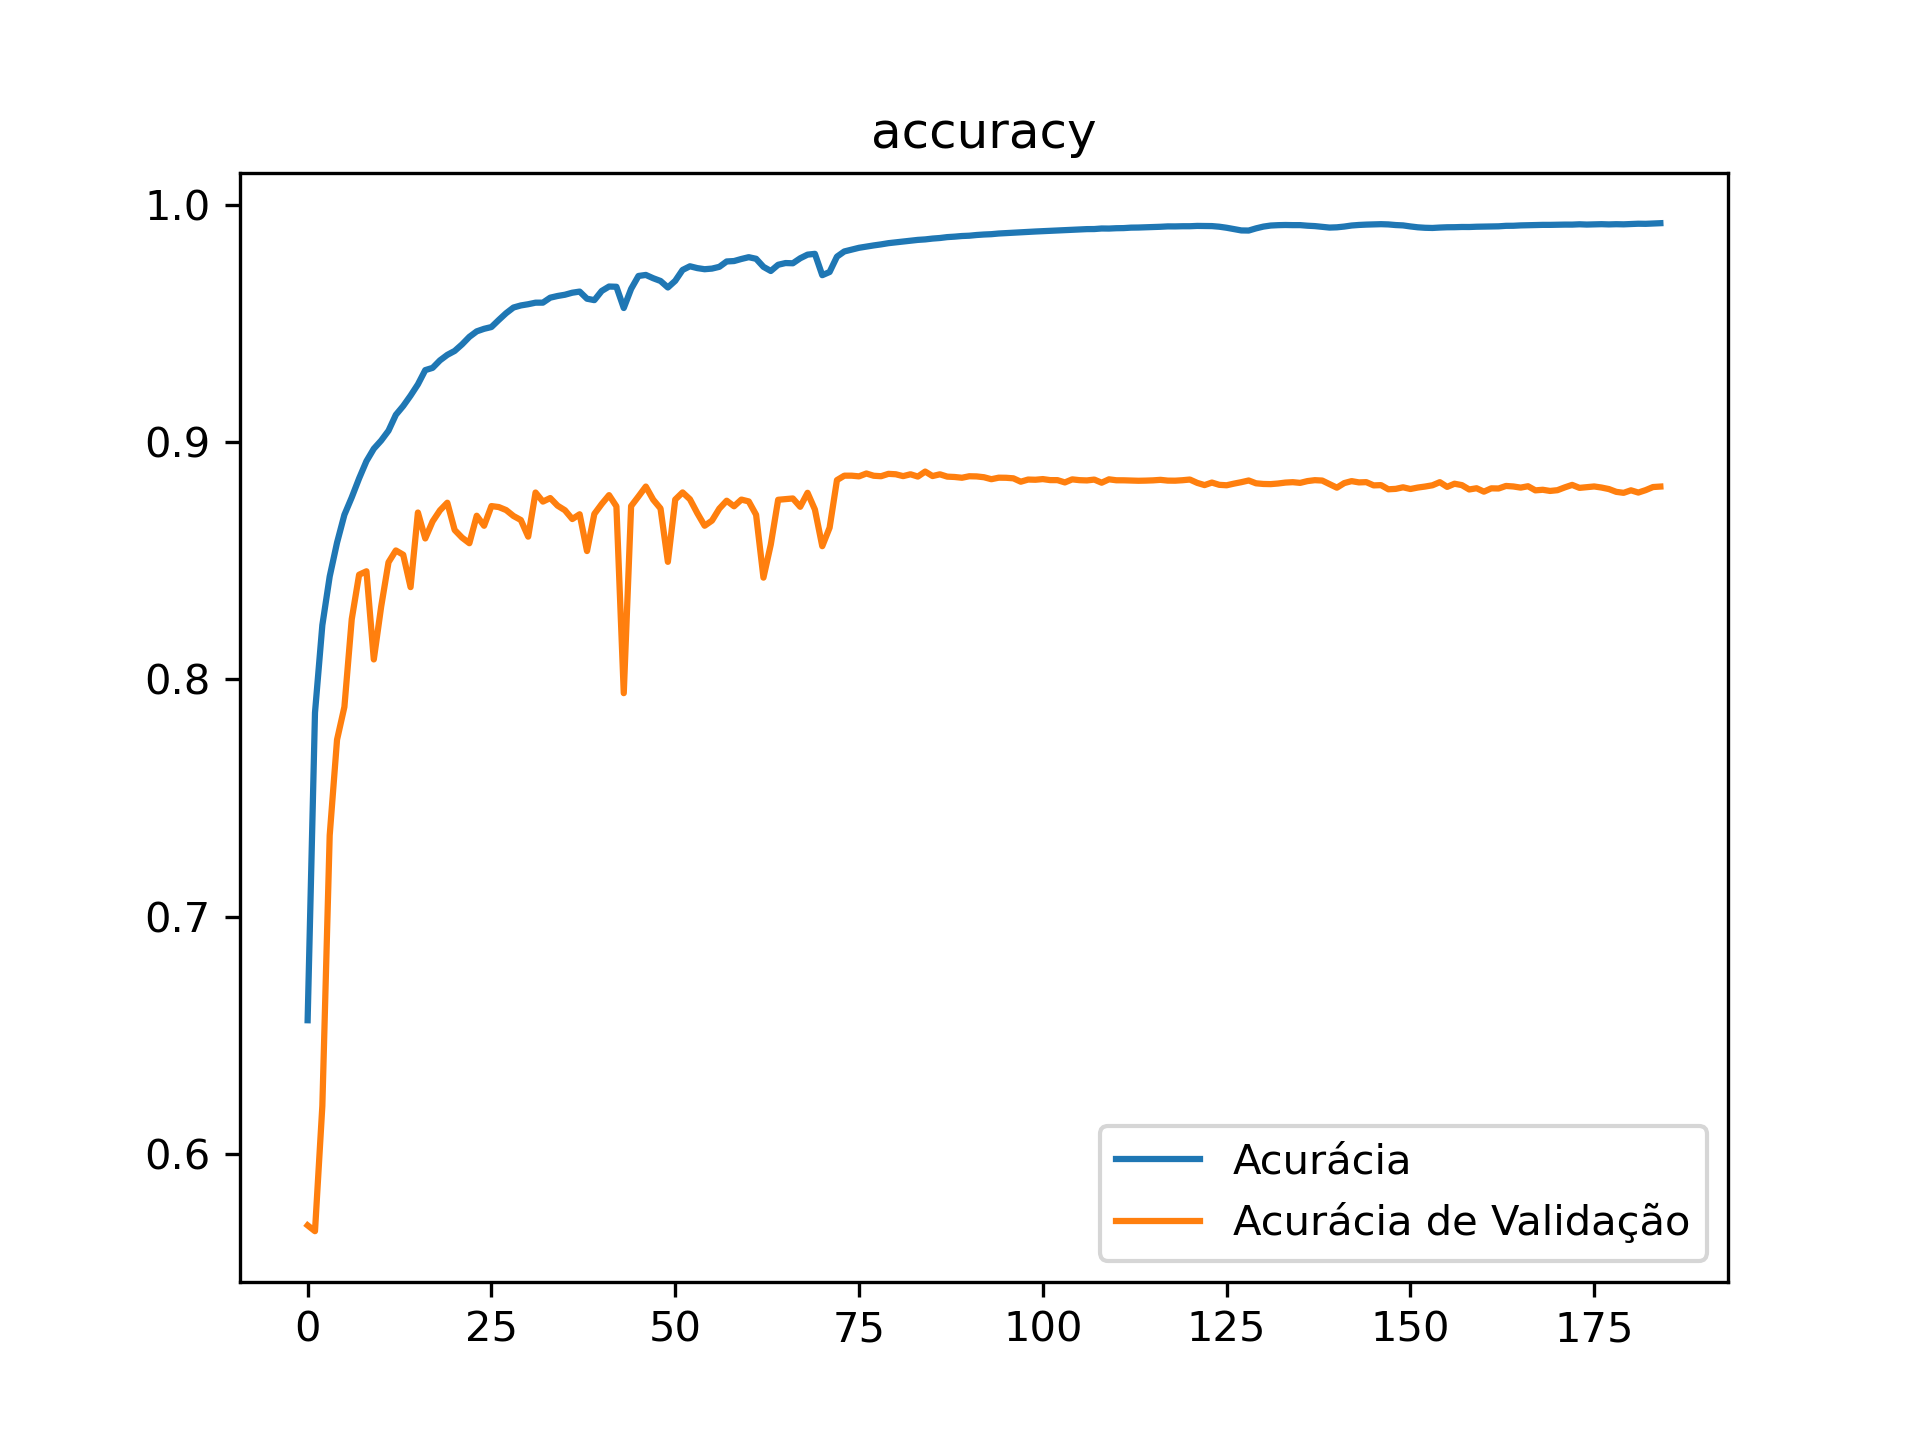
\includegraphics[width=1\linewidth]{recursos/imagens/results/max500_acc_accuracy.png}
         \caption{Acurácia do \textit{Max Pooling}.}
         \label{results:fig:semantic:metrics1.1}
     \end{subfigure}%
     ~ 
     \begin{subfigure}[t]{0.45\textwidth}
         \centering
         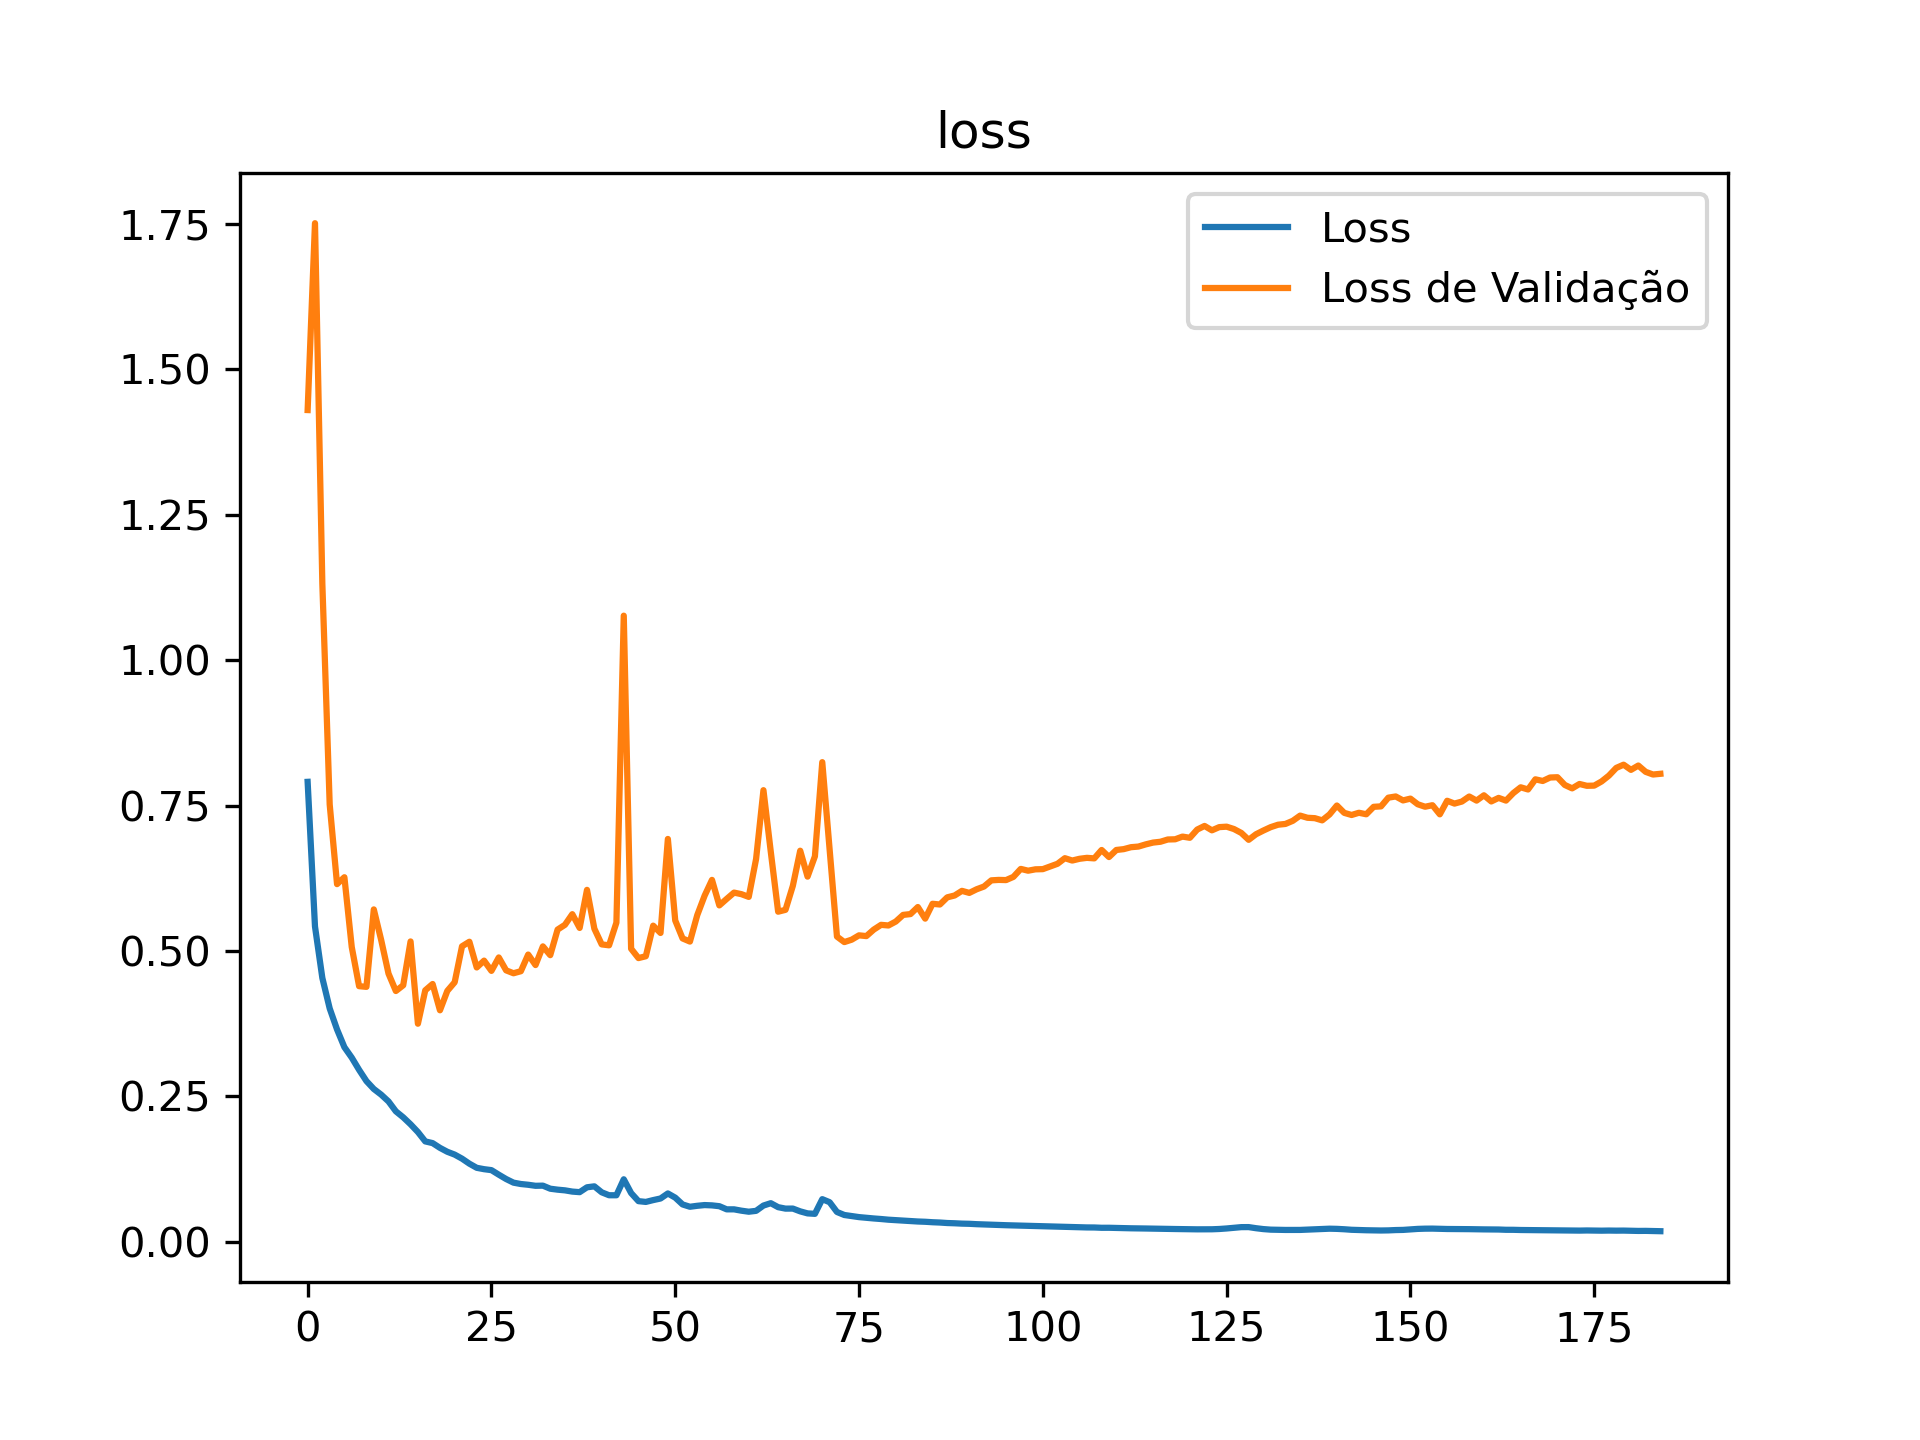
\includegraphics[width=1\linewidth]{recursos/imagens/results/max500_acc_loss.png}
         \caption{\textit{Loss} do \textit{Max Pooling}.}
         \label{results:fig:semantic:metrics1.2}
     \end{subfigure}%
     ~ 
     
     \begin{subfigure}[t]{0.45\textwidth}
         \centering
         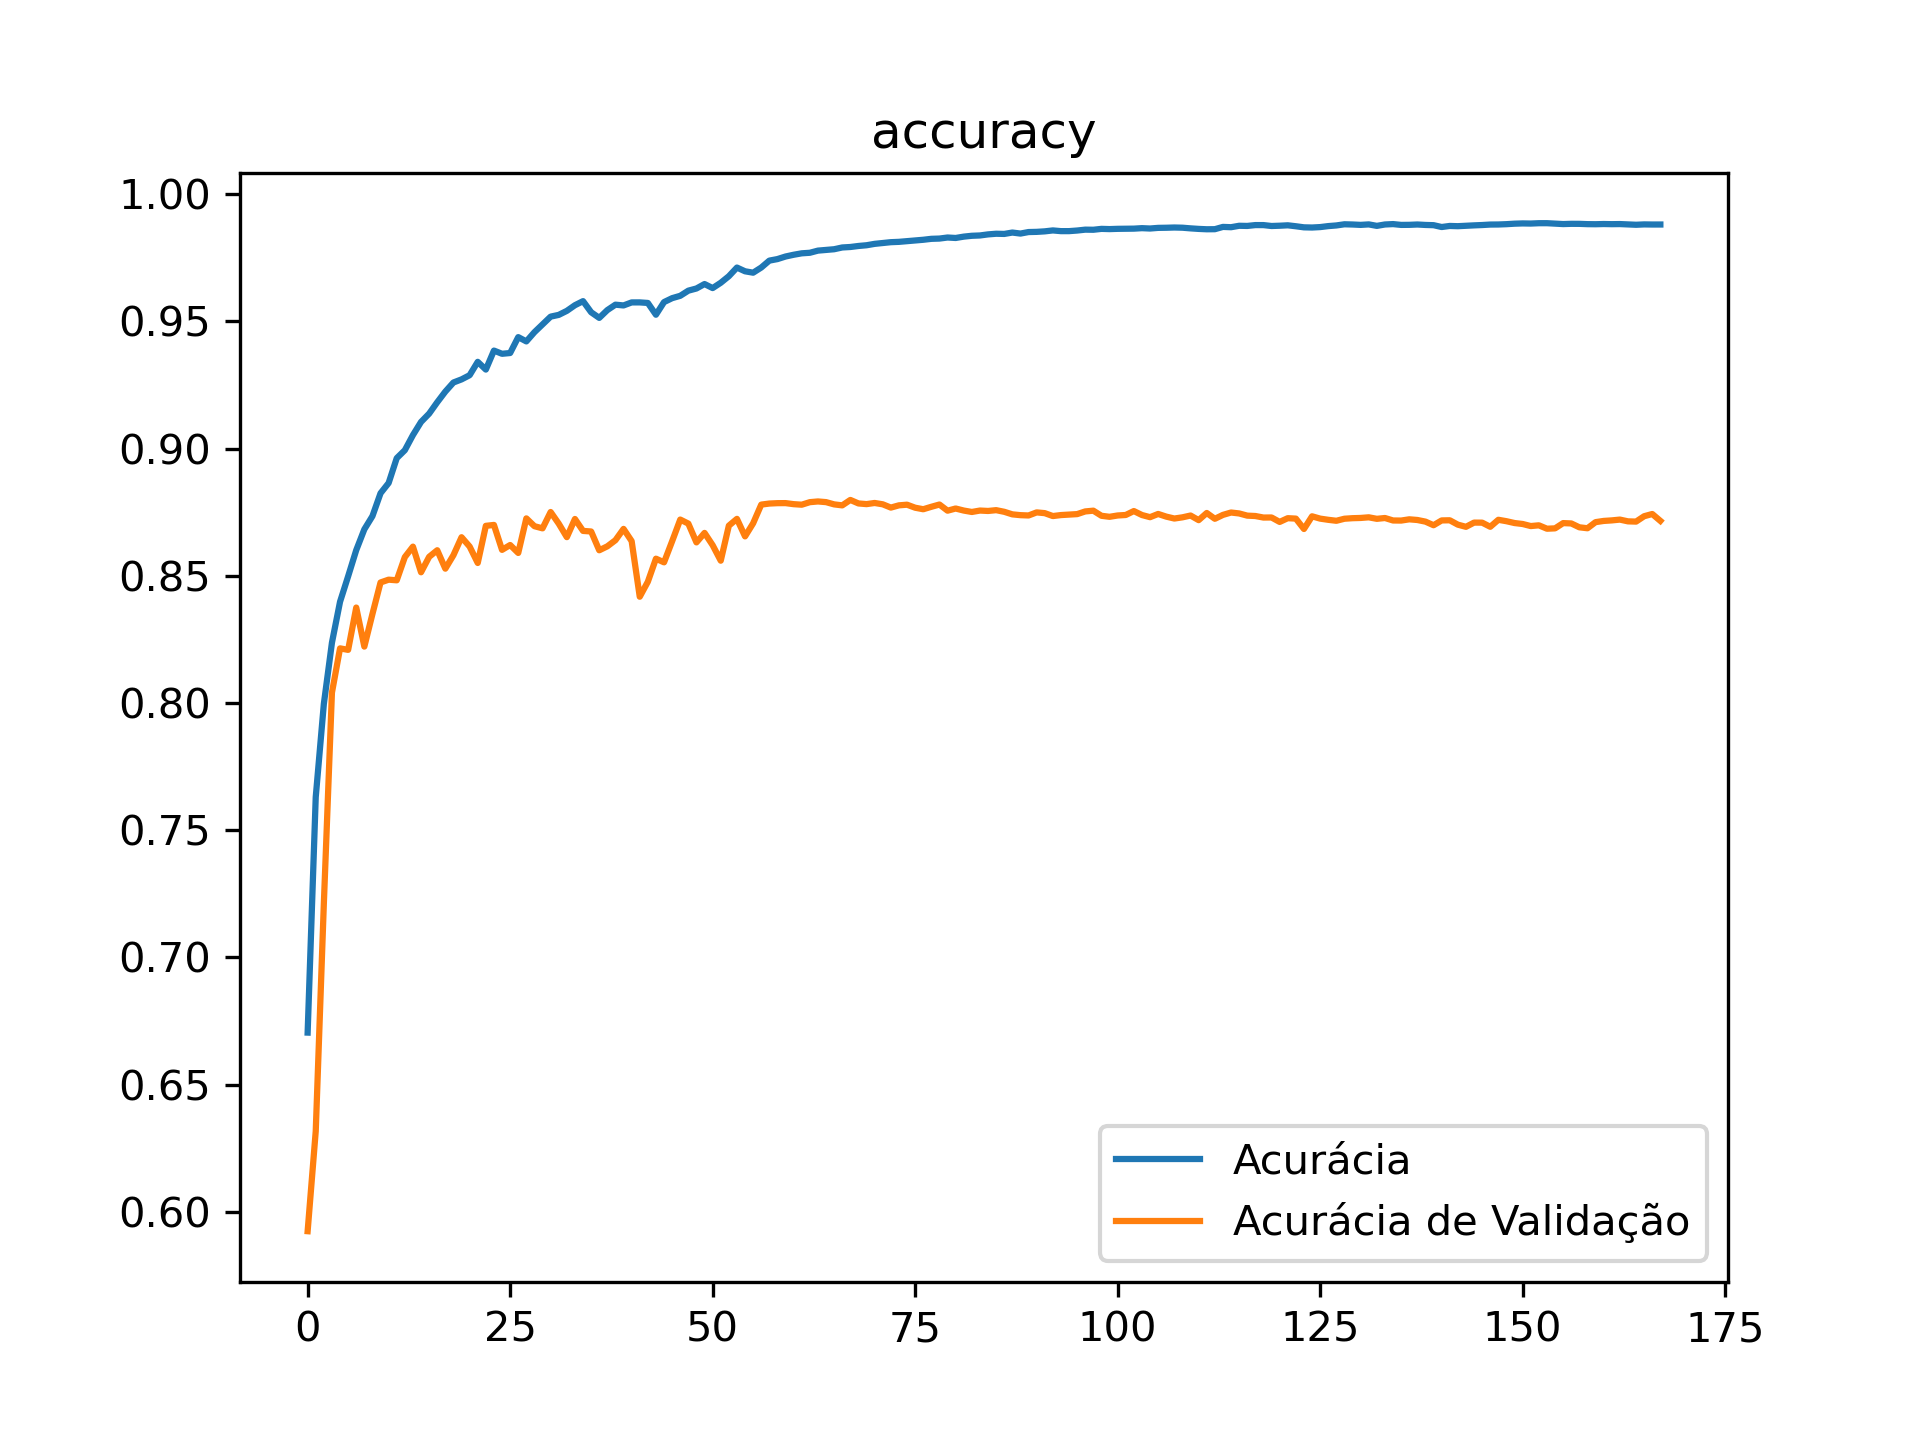
\includegraphics[width=1\linewidth]{recursos/imagens/results/bpca500_acc_accuracy.png}
         \caption{Acurácia do BPCAPooling.}
         \label{results:fig:semantic:metrics1.3}
     \end{subfigure}
     ~
     \begin{subfigure}[t]{0.45\textwidth}
         \centering
         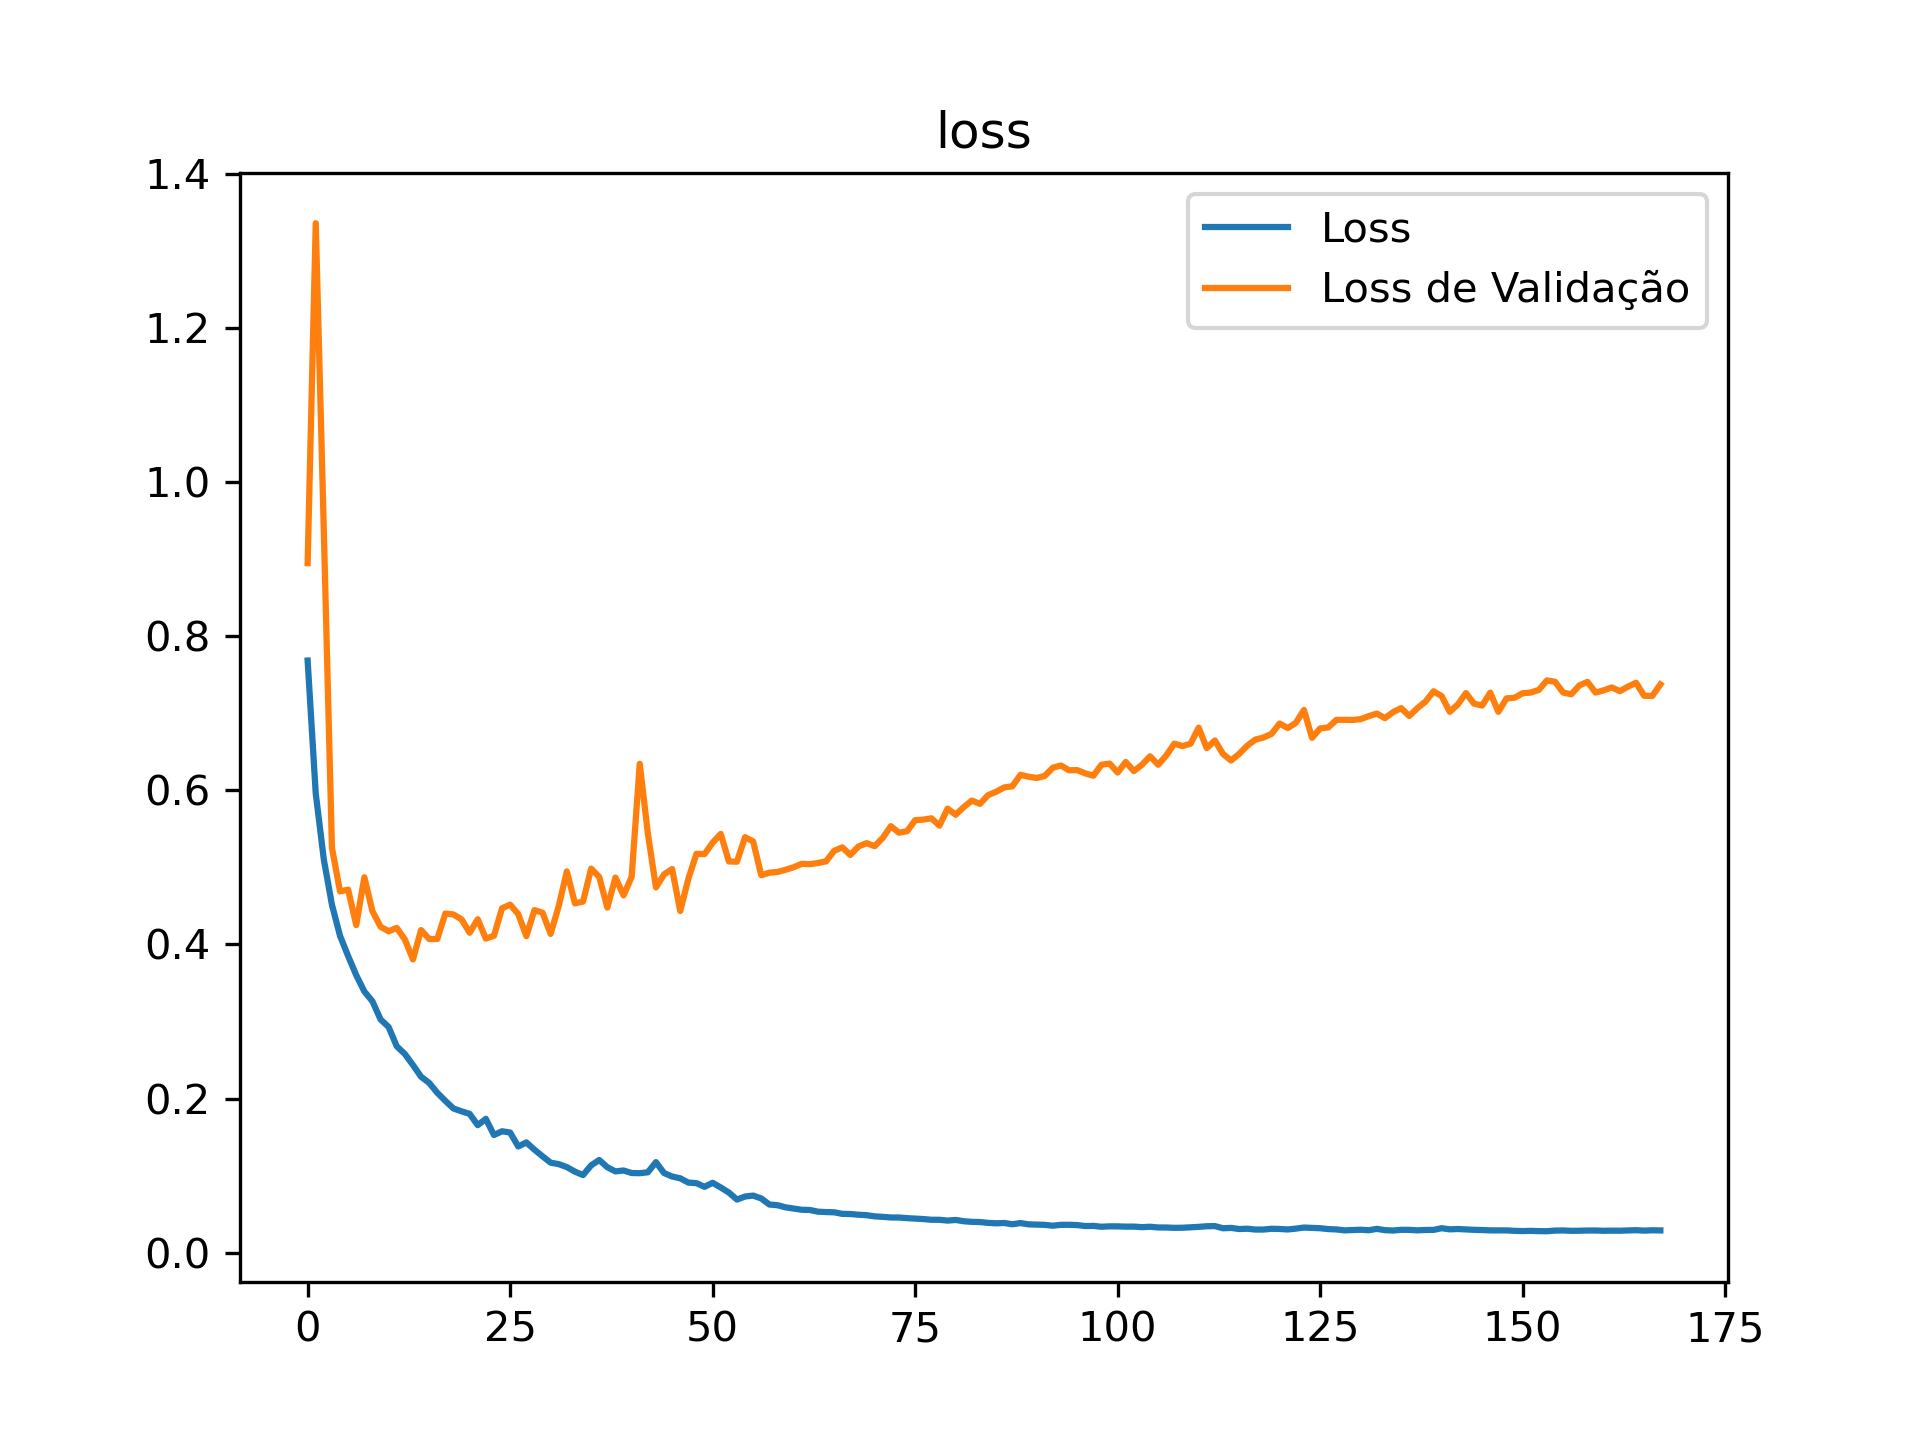
\includegraphics[width=1\linewidth]{recursos/imagens/results/bpca500_acc_loss.png}
         \caption{\textit{Loss} do BPCAPooling.}
         \label{results:fig:semantic:metrics1.4}
     \end{subfigure}
     
     Fonte: do próprio autor.
\end{figure}

\begin{figure}[H]
    \centering
    \caption{Métricas de U-Net com BPCAPooling e 500 épocas no conjunto de dados \textit{Oxford-IIIT Pets} baseada em mIoU.}
    \label{results:fig:semantic:metrics2}
     \begin{subfigure}[t]{0.45\textwidth}
         \centering
         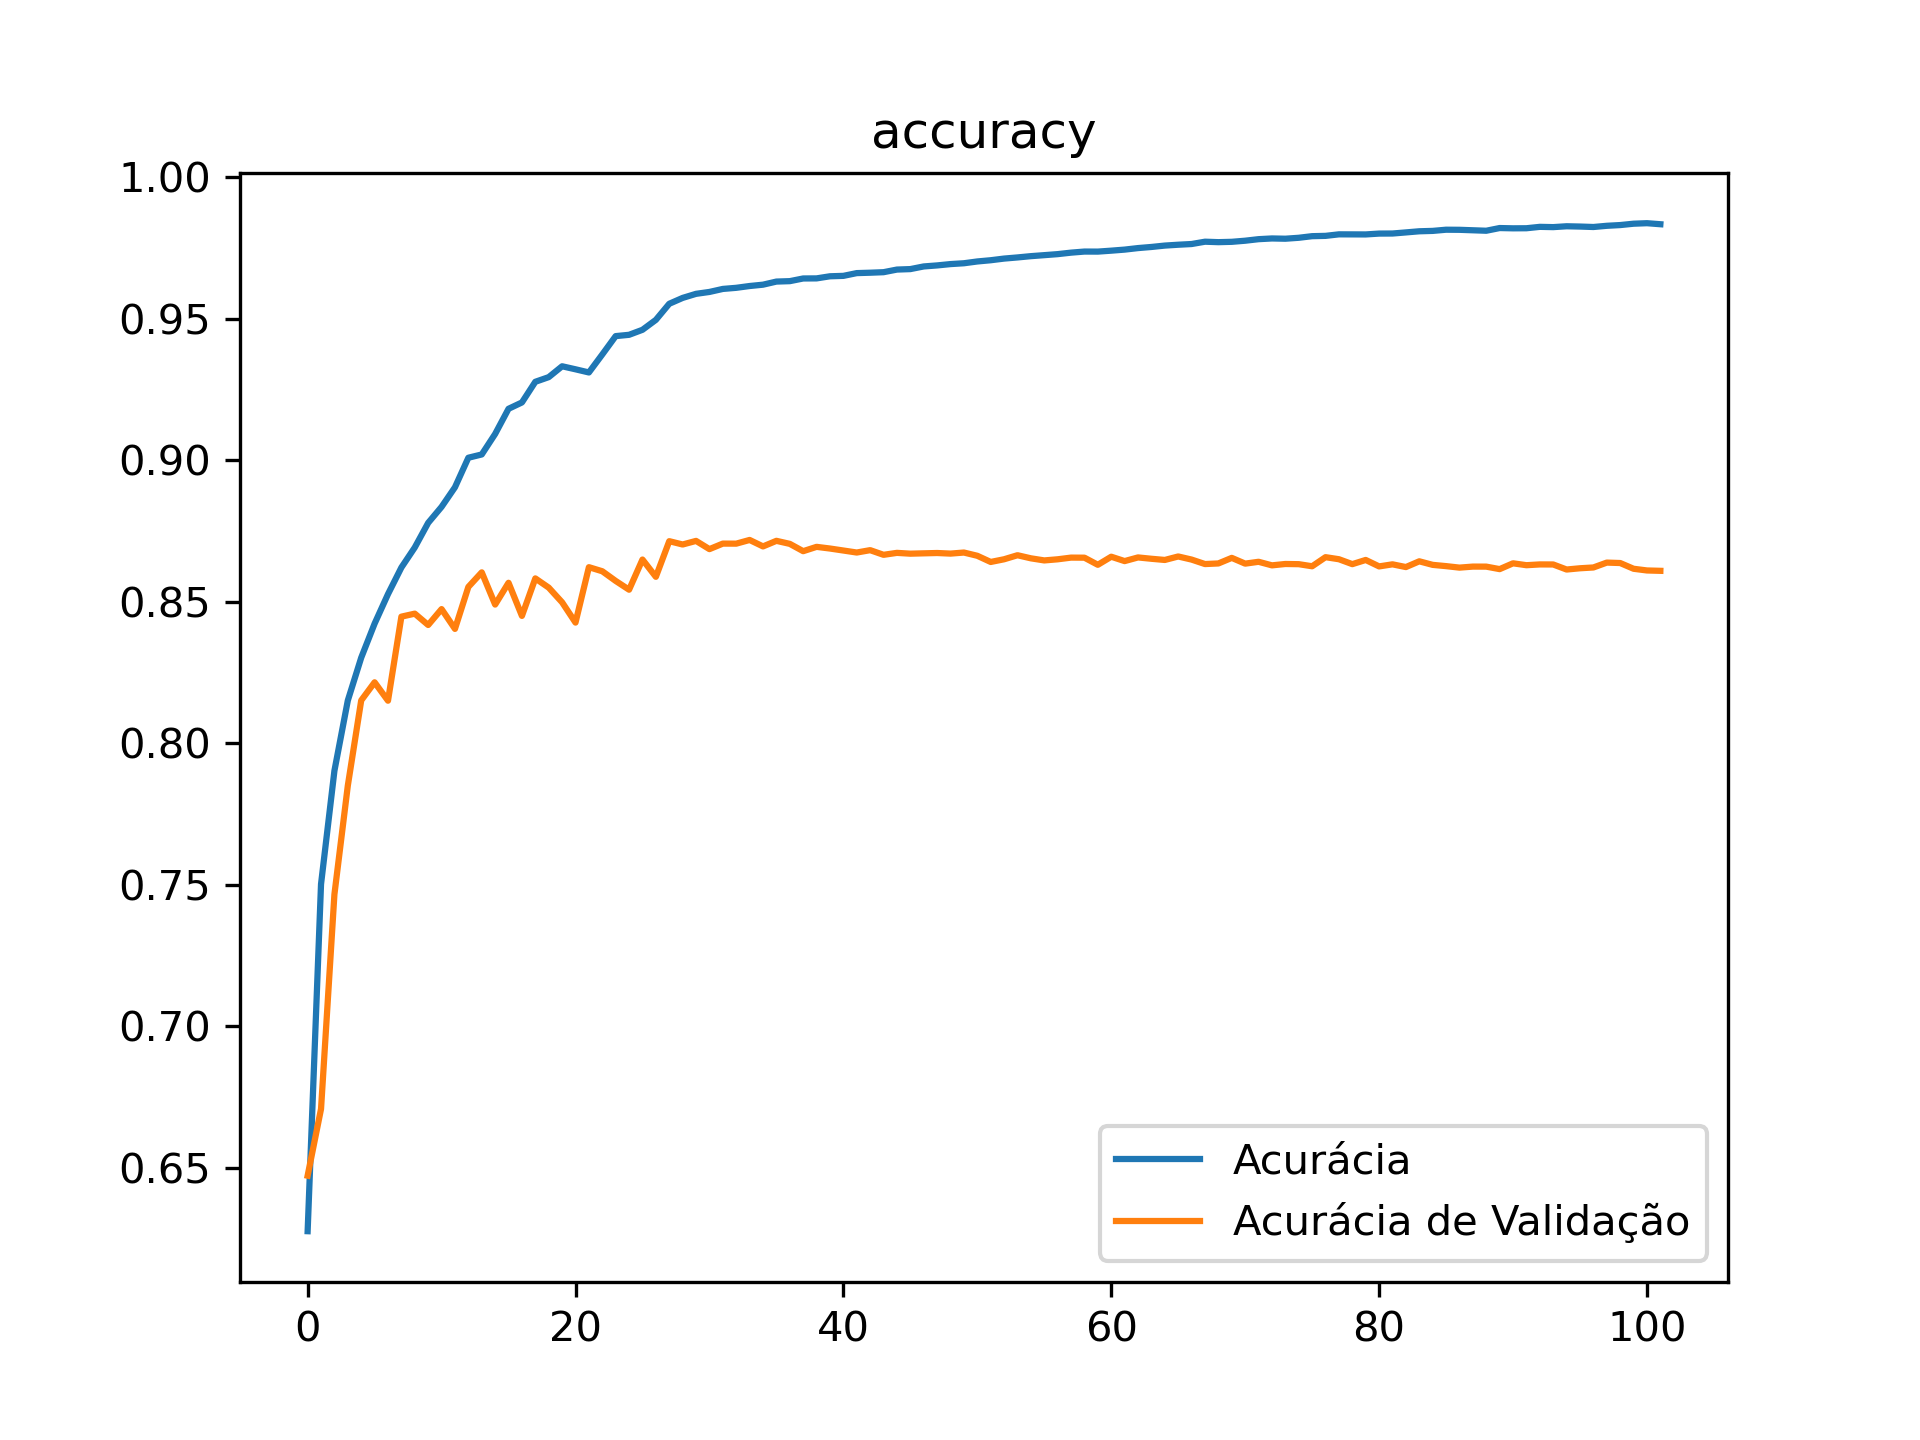
\includegraphics[width=1\linewidth]{recursos/imagens/results/bpca_unet500_miou_accuracy.png}
         \caption{Acurácia.}
         \label{results:fig:semantic:metrics2.1}
     \end{subfigure}%
     ~ 
     \begin{subfigure}[t]{0.45\textwidth}
         \centering
         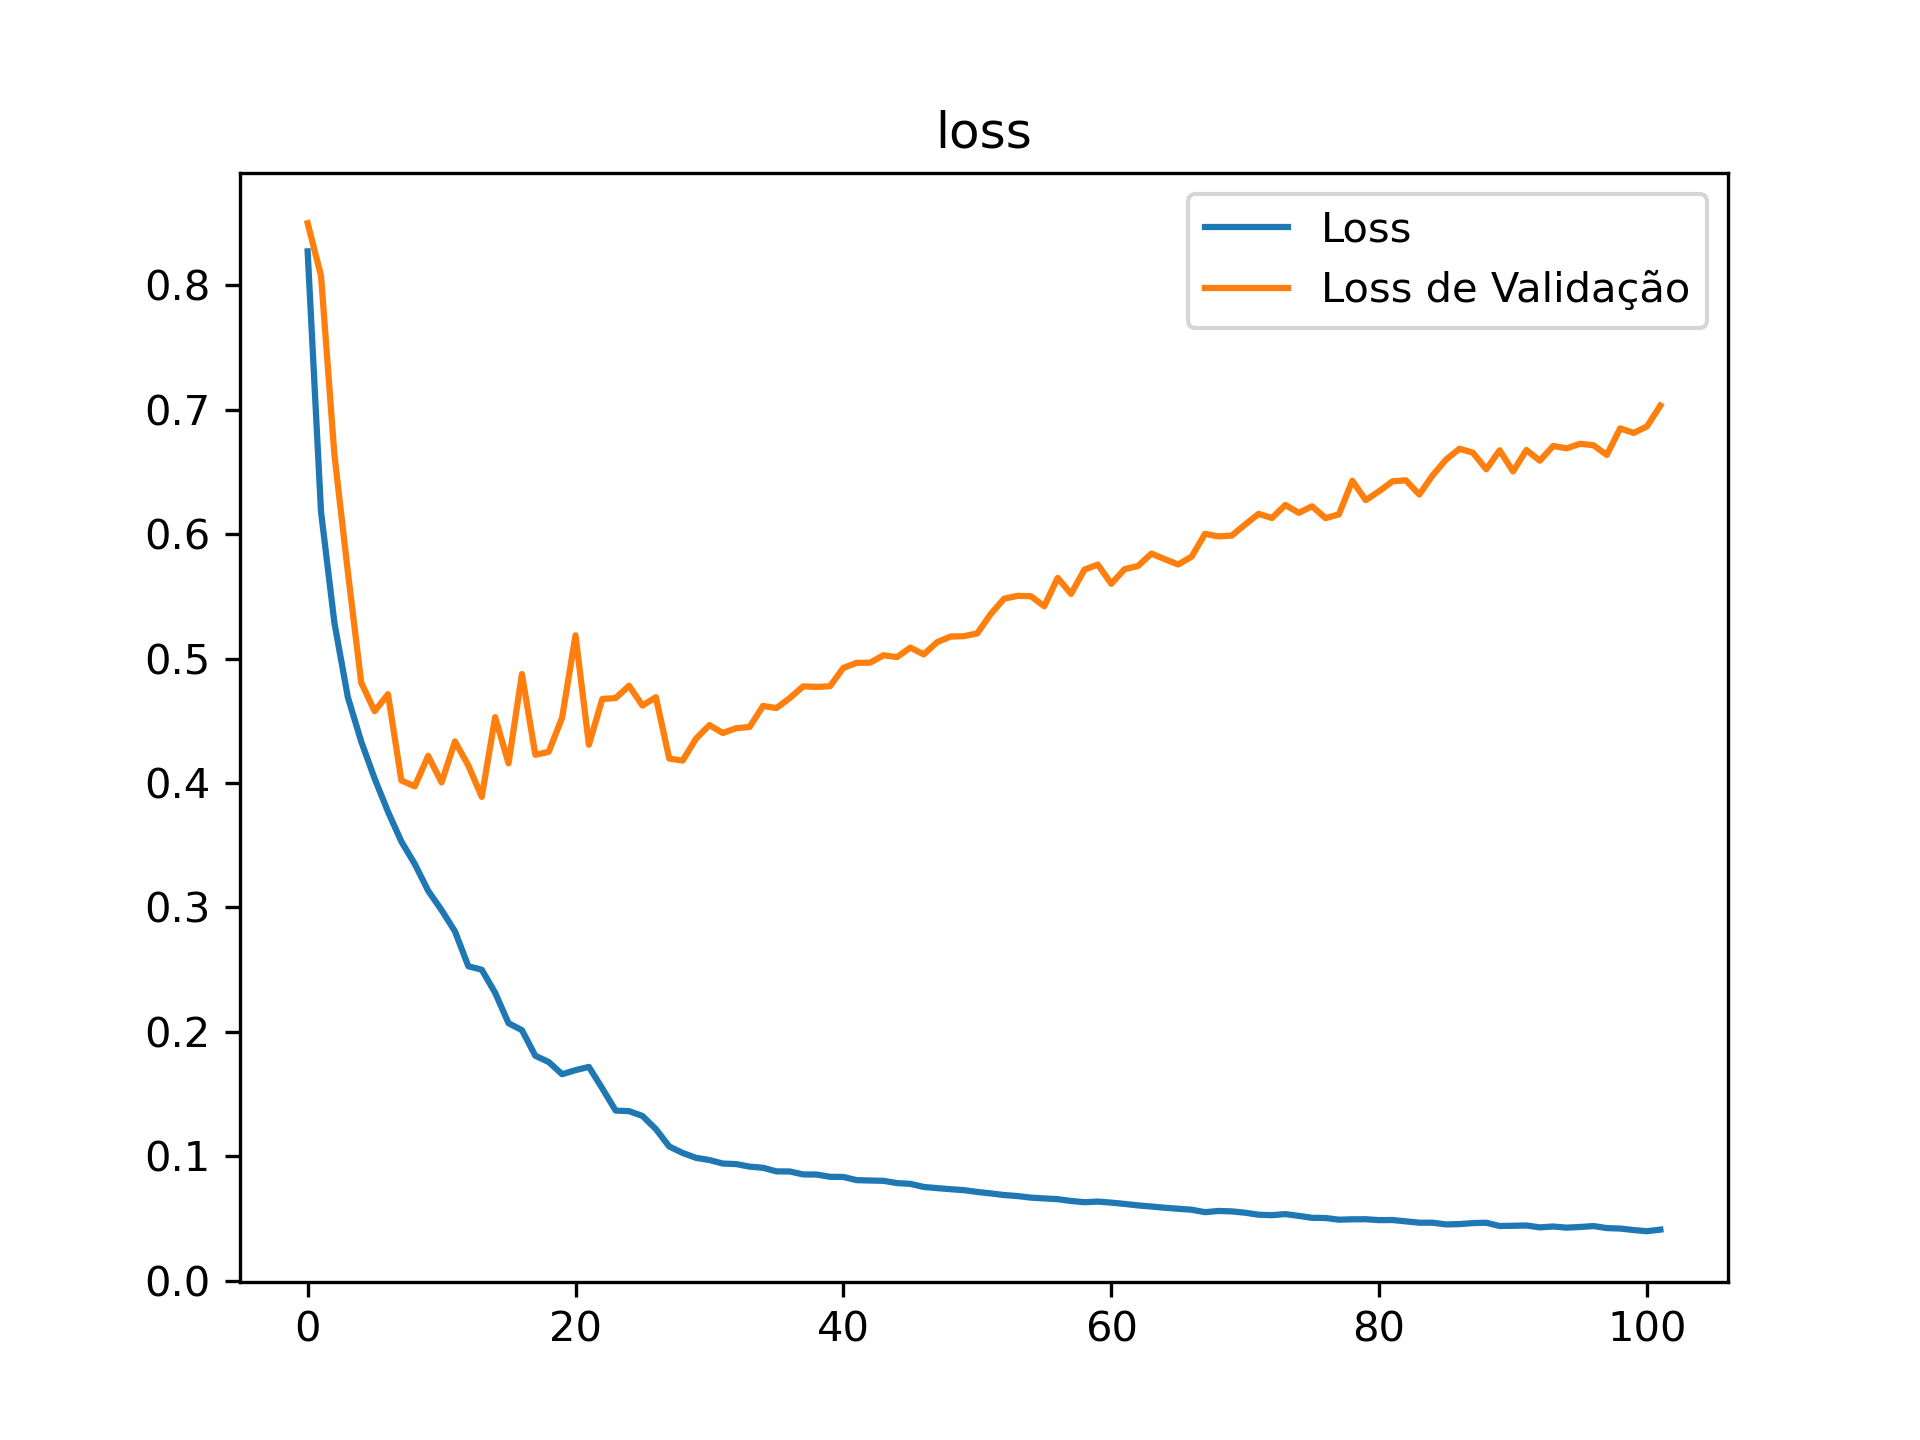
\includegraphics[width=1\linewidth]{recursos/imagens/results/bpca_unet500_miou_loss.png}
         \caption{\textit{Loss}.}
         \label{results:fig:semantic:metrics2.2}
     \end{subfigure}%
     ~ 
     
     \begin{subfigure}[t]{0.45\textwidth}
         \centering
         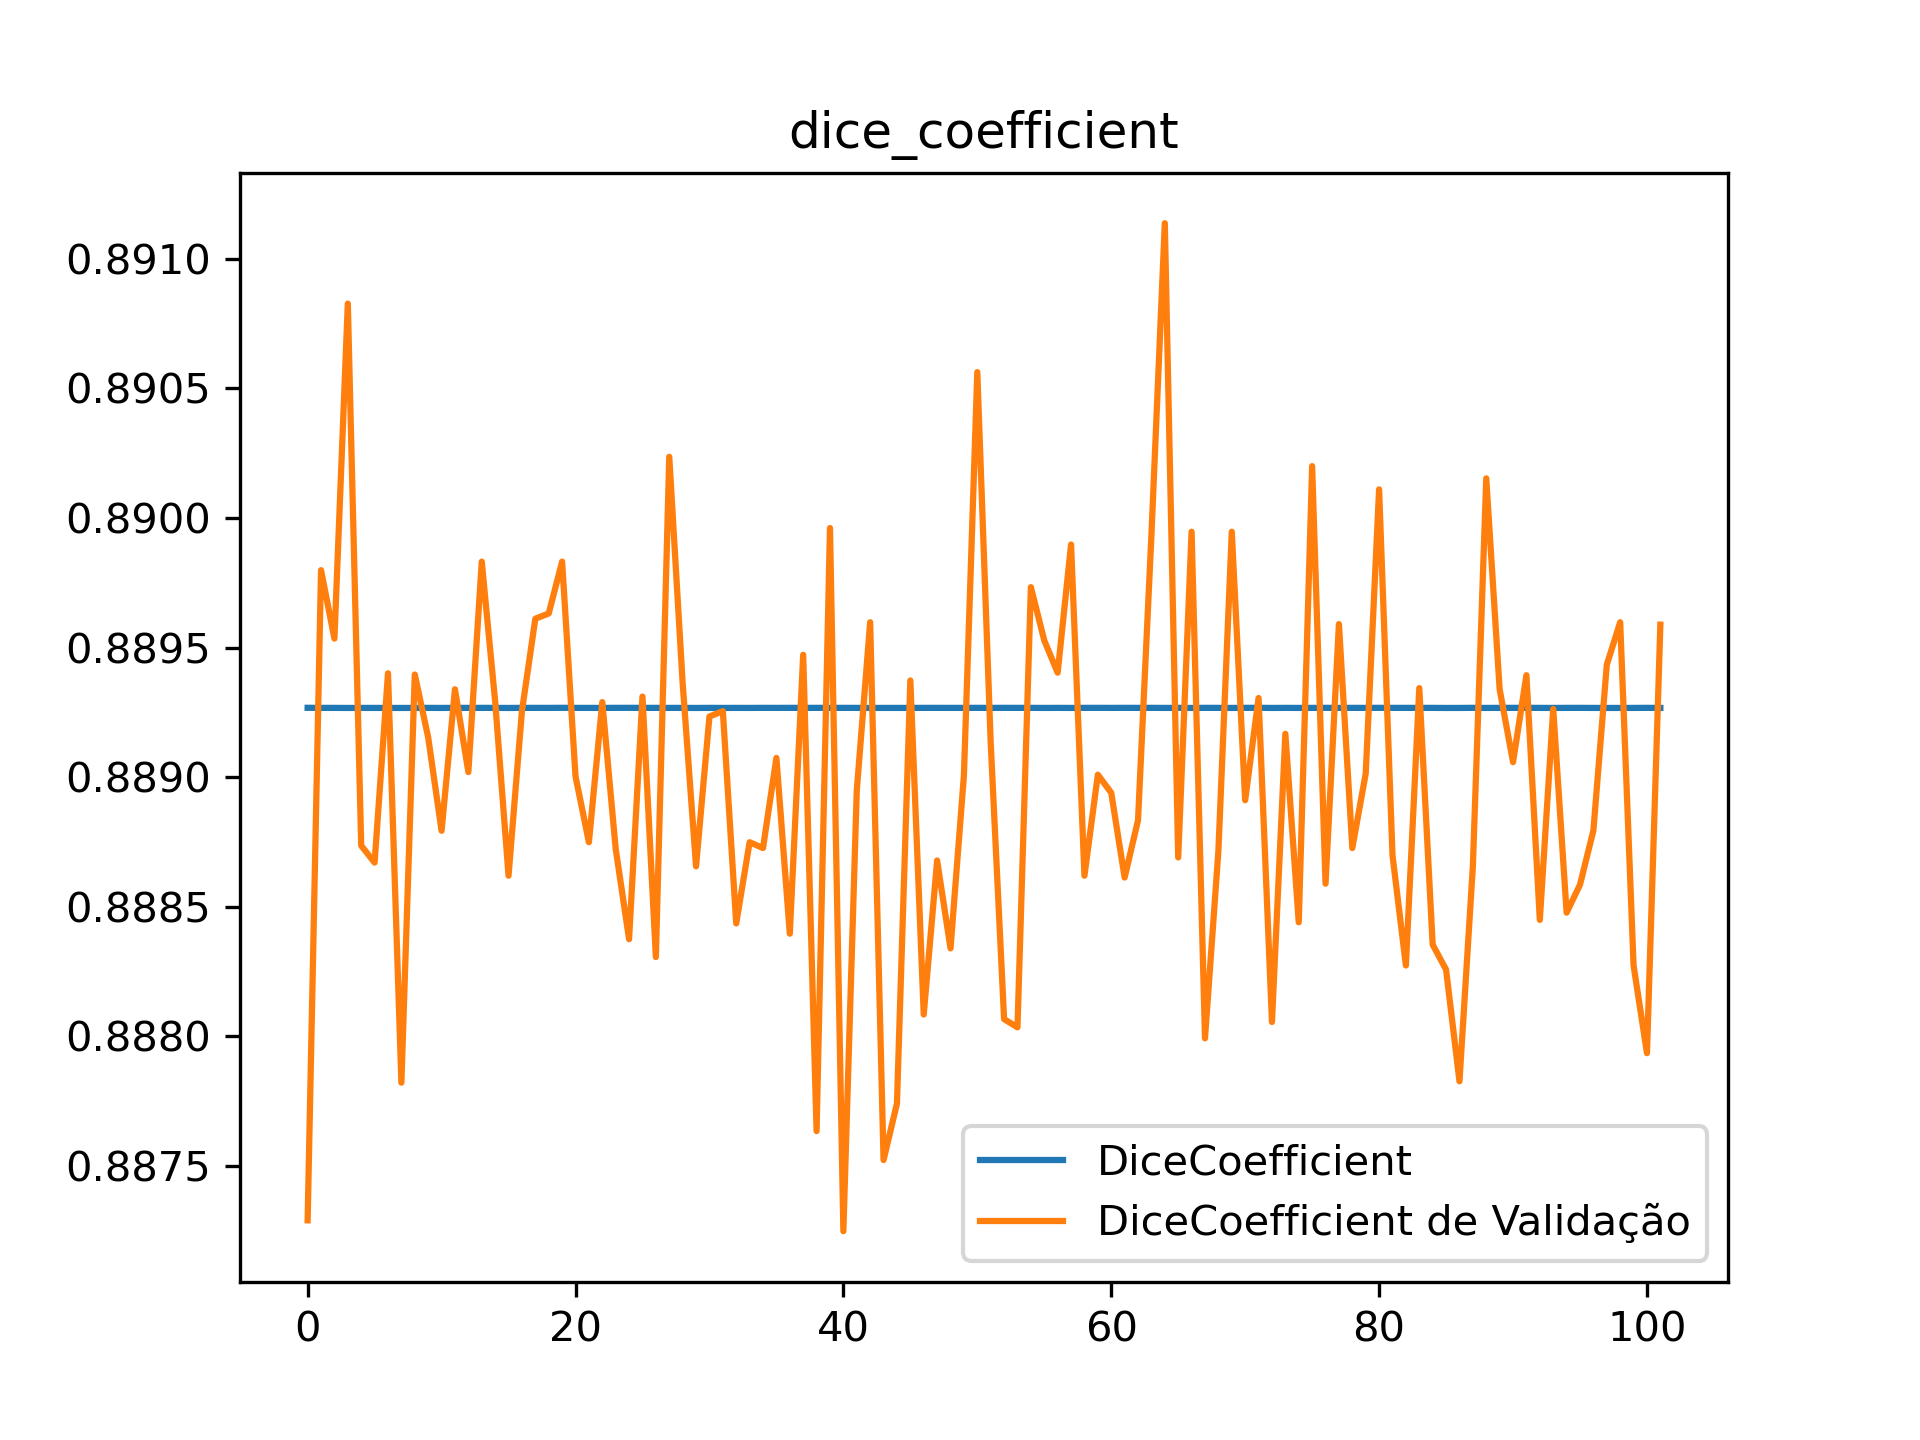
\includegraphics[width=1\linewidth]{recursos/imagens/results/bpca_unet500_miou_dice_coefficient.png}
         \caption{Dice.}
         \label{results:fig:semantic:metrics2.3}
     \end{subfigure}
     ~
     \begin{subfigure}[t]{0.45\textwidth}
         \centering
         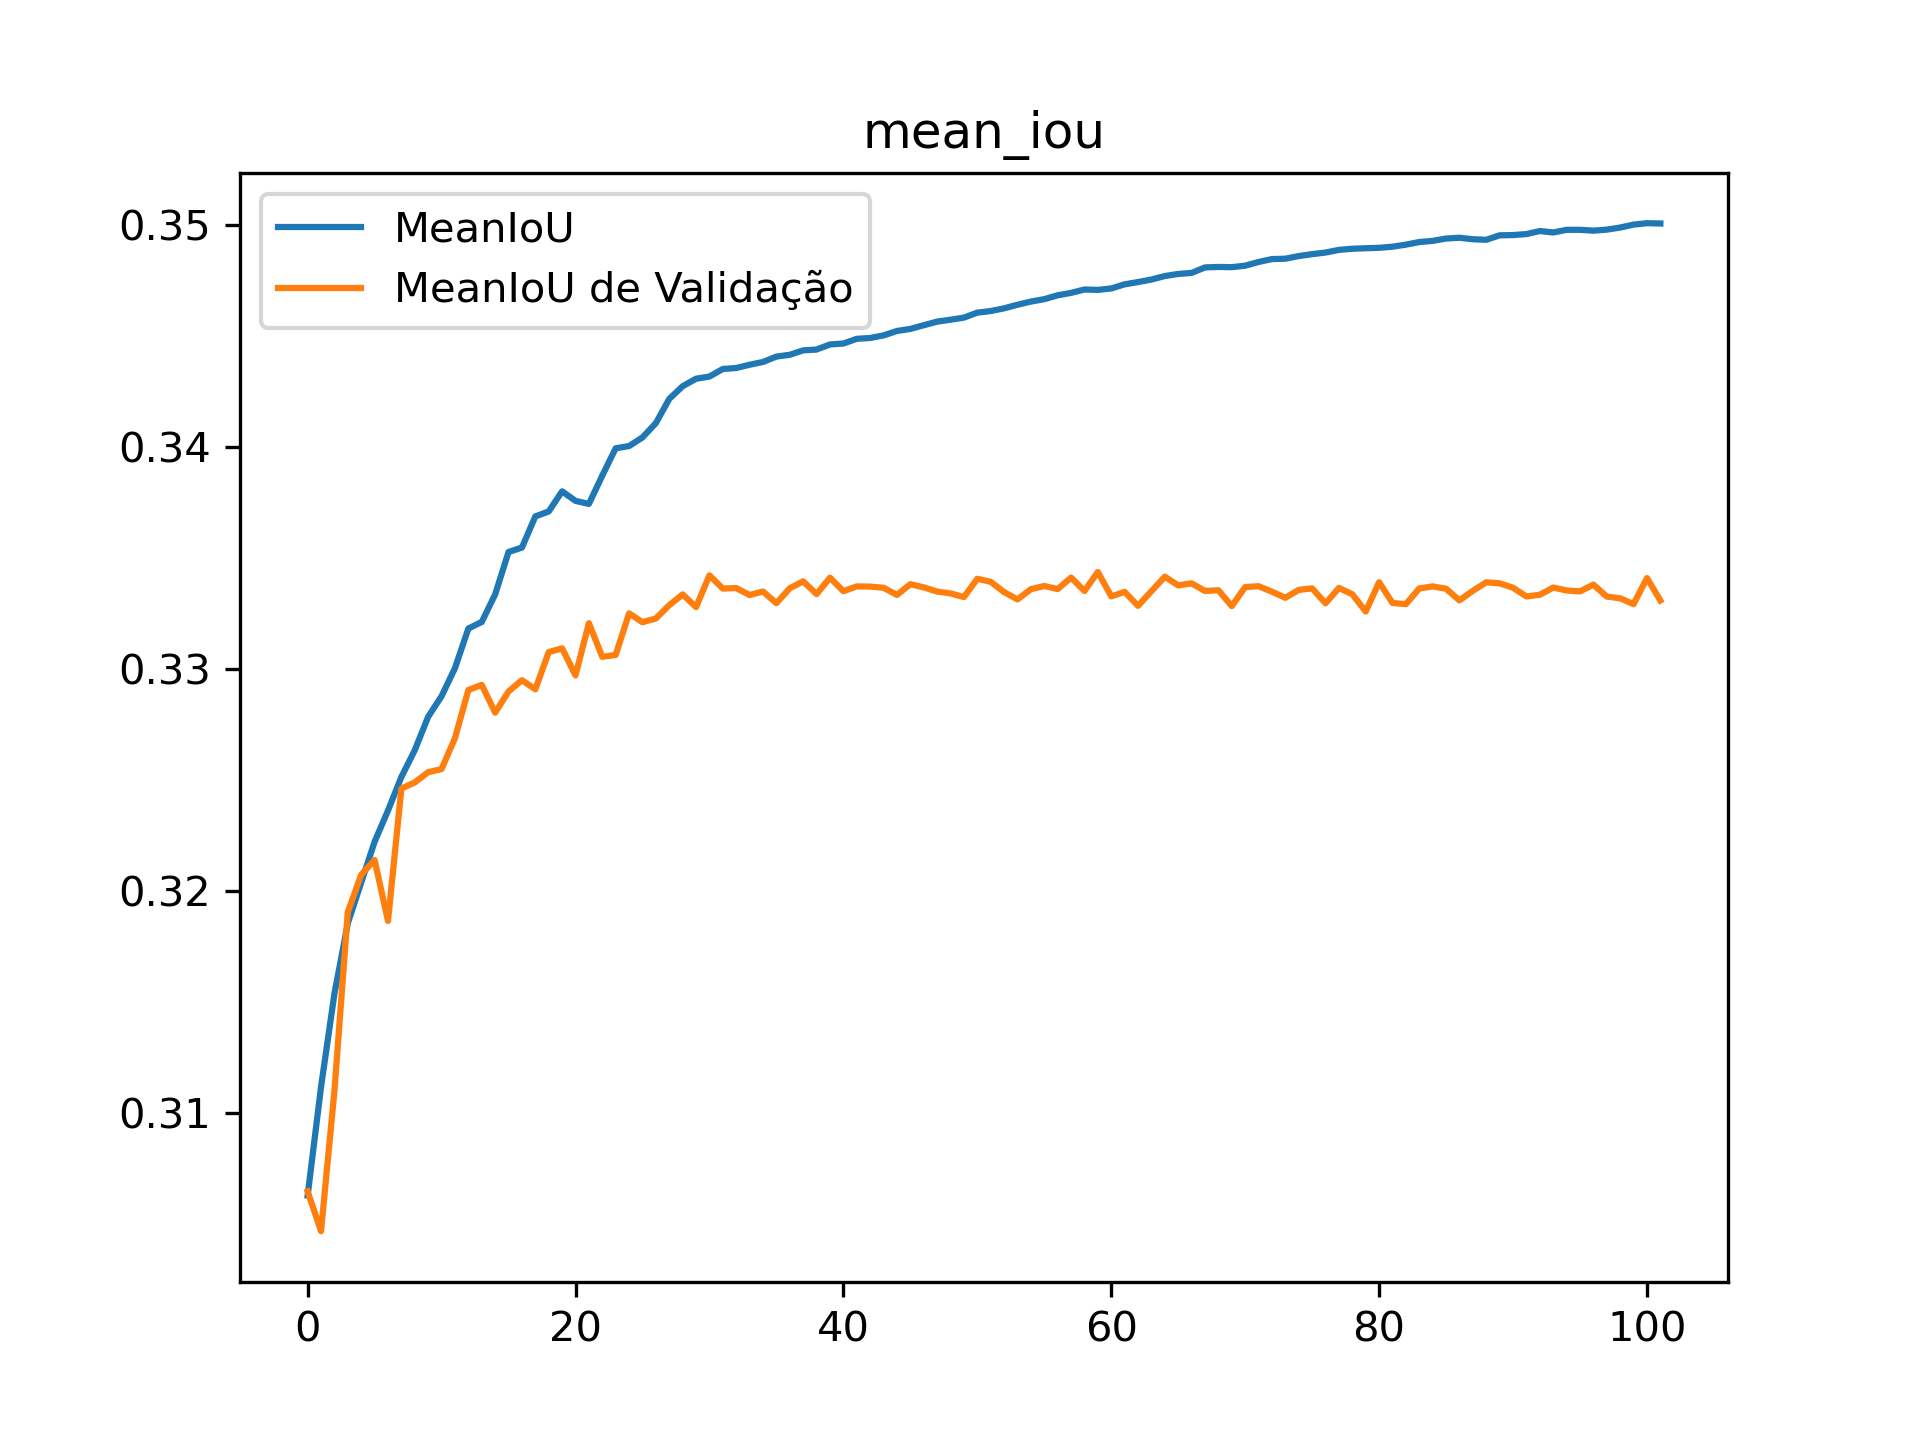
\includegraphics[width=1\linewidth]{recursos/imagens/results/bpca_unet500_miou_mean_iou.png}
         \caption{mIoU.}
         \label{results:fig:semantic:metrics2.4}
     \end{subfigure}
     
     Fonte: do próprio autor.
\end{figure}

\begin{figure}[H]
    \centering
    \caption{Métricas de U-Net com \textit{Max Pooling} e 500 épocas no conjunto de dados \textit{Oxford-IIIT Pets} baseada em mIoU.}
    \label{results:fig:semantic:metrics3}
     \begin{subfigure}[t]{0.45\textwidth}
         \centering
         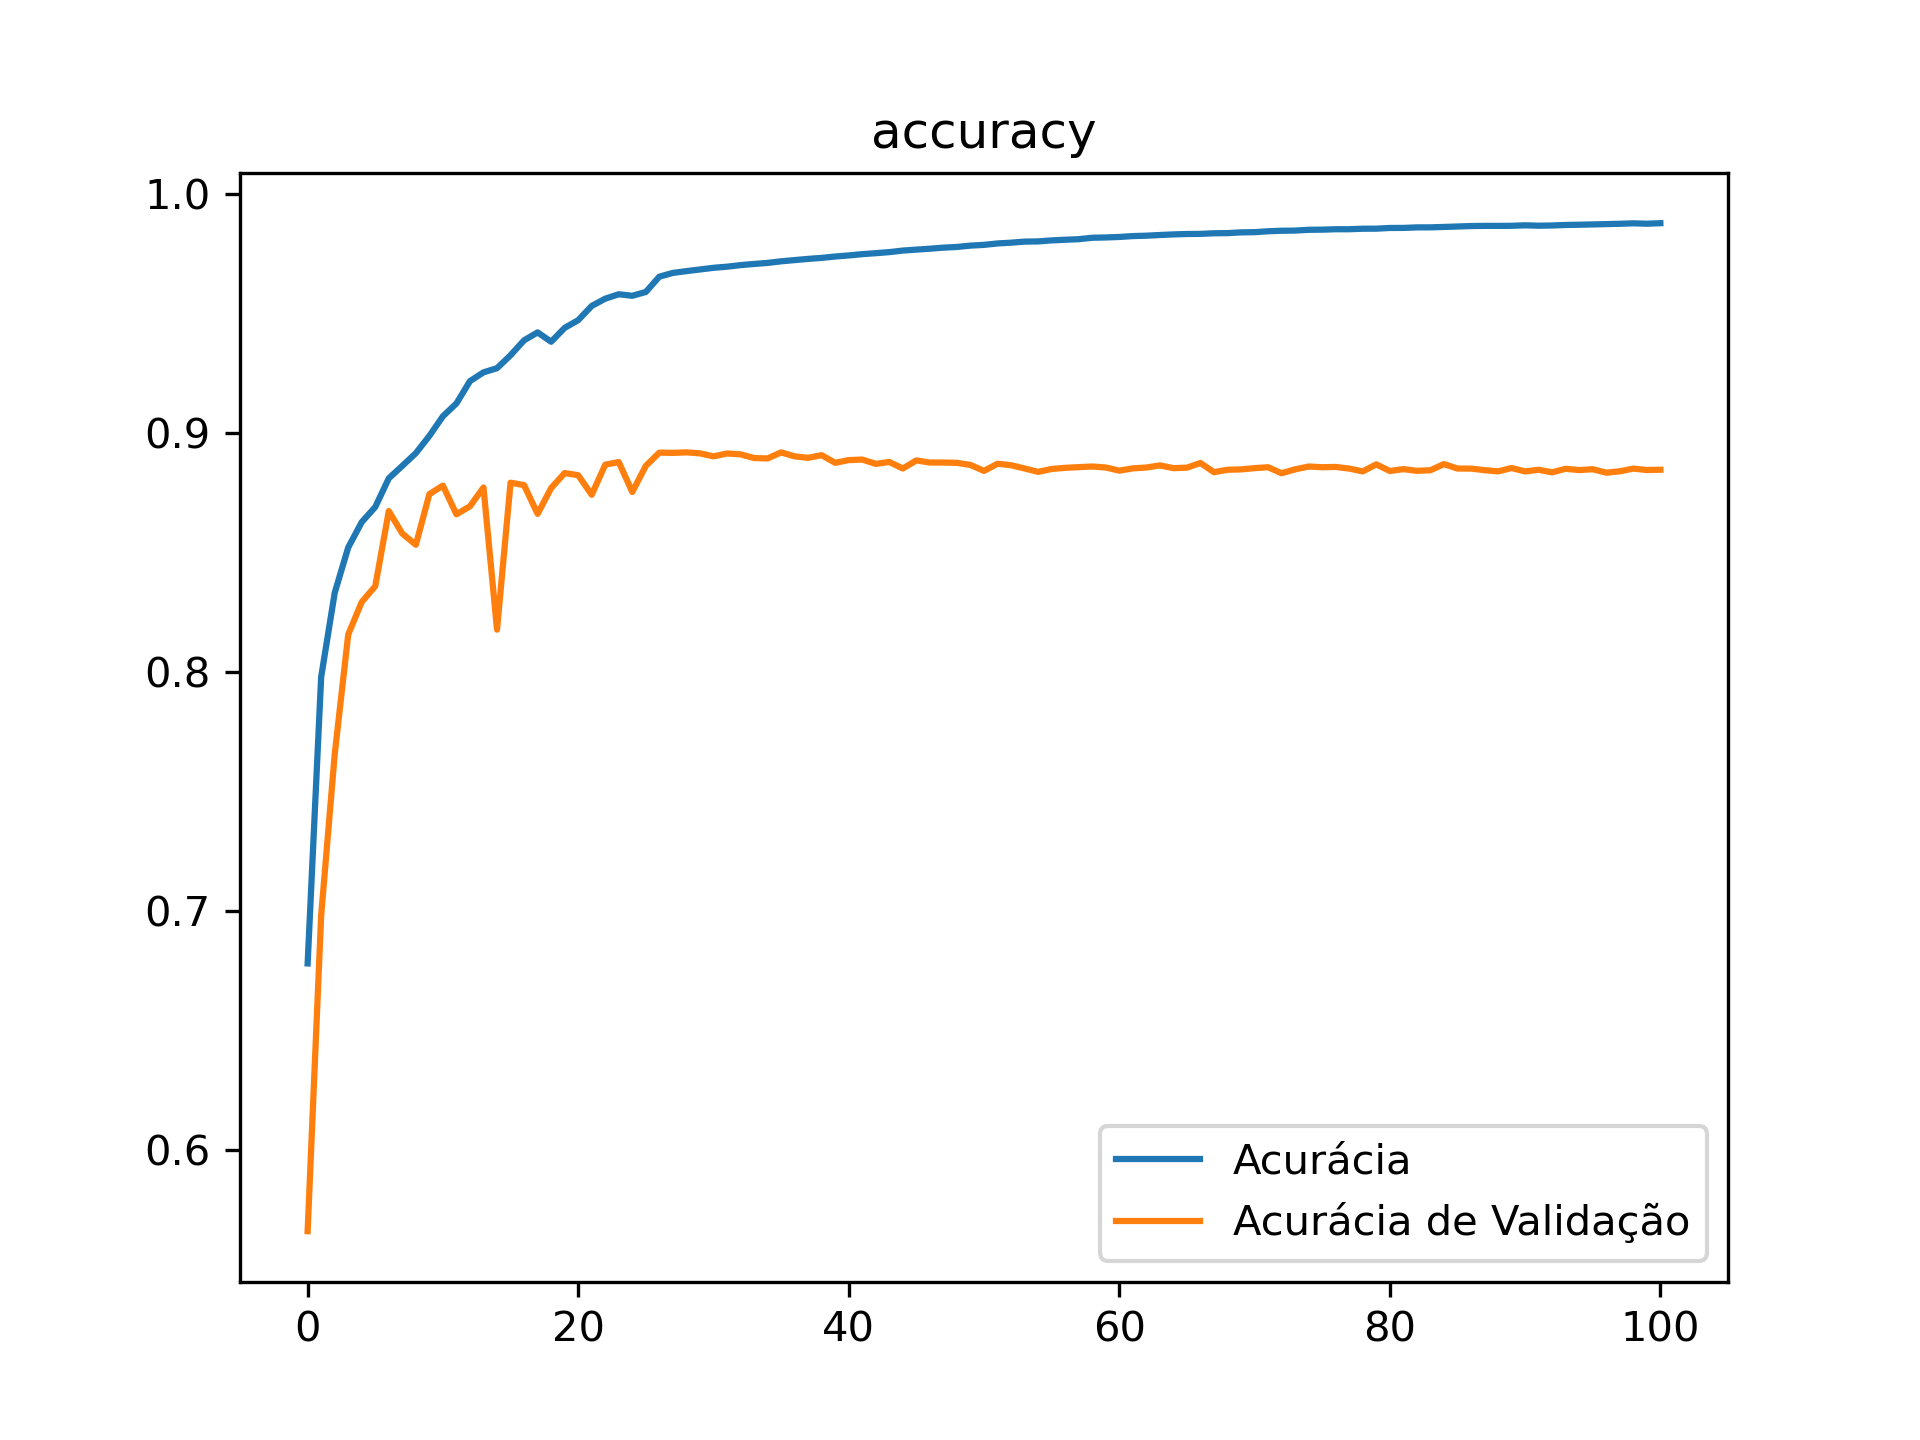
\includegraphics[width=1\linewidth]{recursos/imagens/results/max_unet500_miou_accuracy.png}
         \caption{Acurácia.}
         \label{results:fig:semantic:metrics3.1}
     \end{subfigure}%
     ~ 
     \begin{subfigure}[t]{0.45\textwidth}
         \centering
         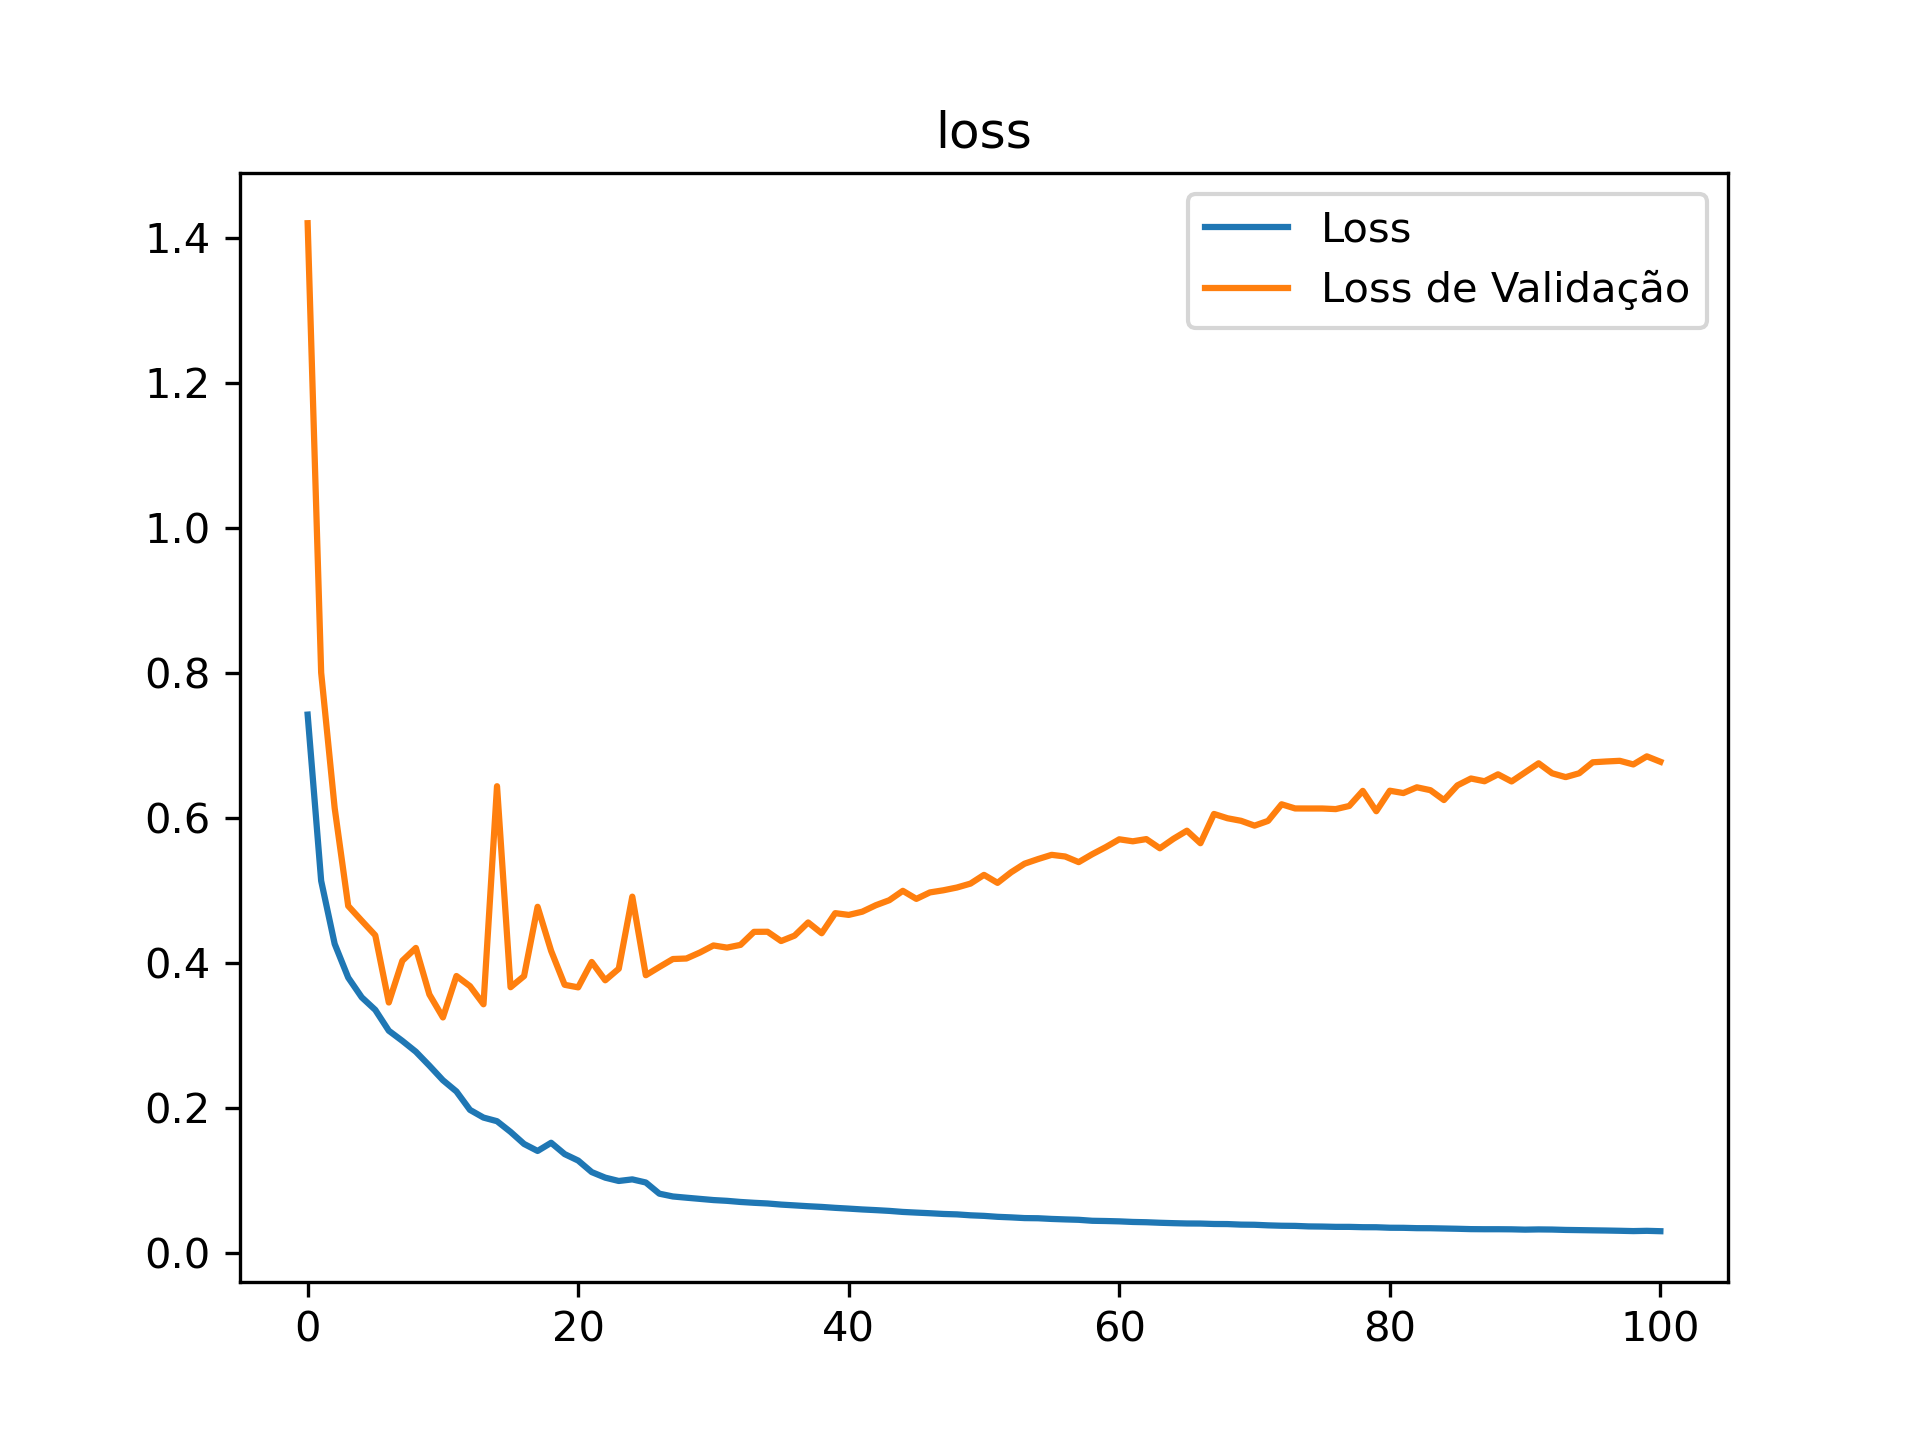
\includegraphics[width=1\linewidth]{recursos/imagens/results/max_unet500_miou_loss.png}
         \caption{\textit{Loss}.}
         \label{results:fig:semantic:metrics3.2}
     \end{subfigure}%
     ~ 
     
     \begin{subfigure}[t]{0.45\textwidth}
         \centering
         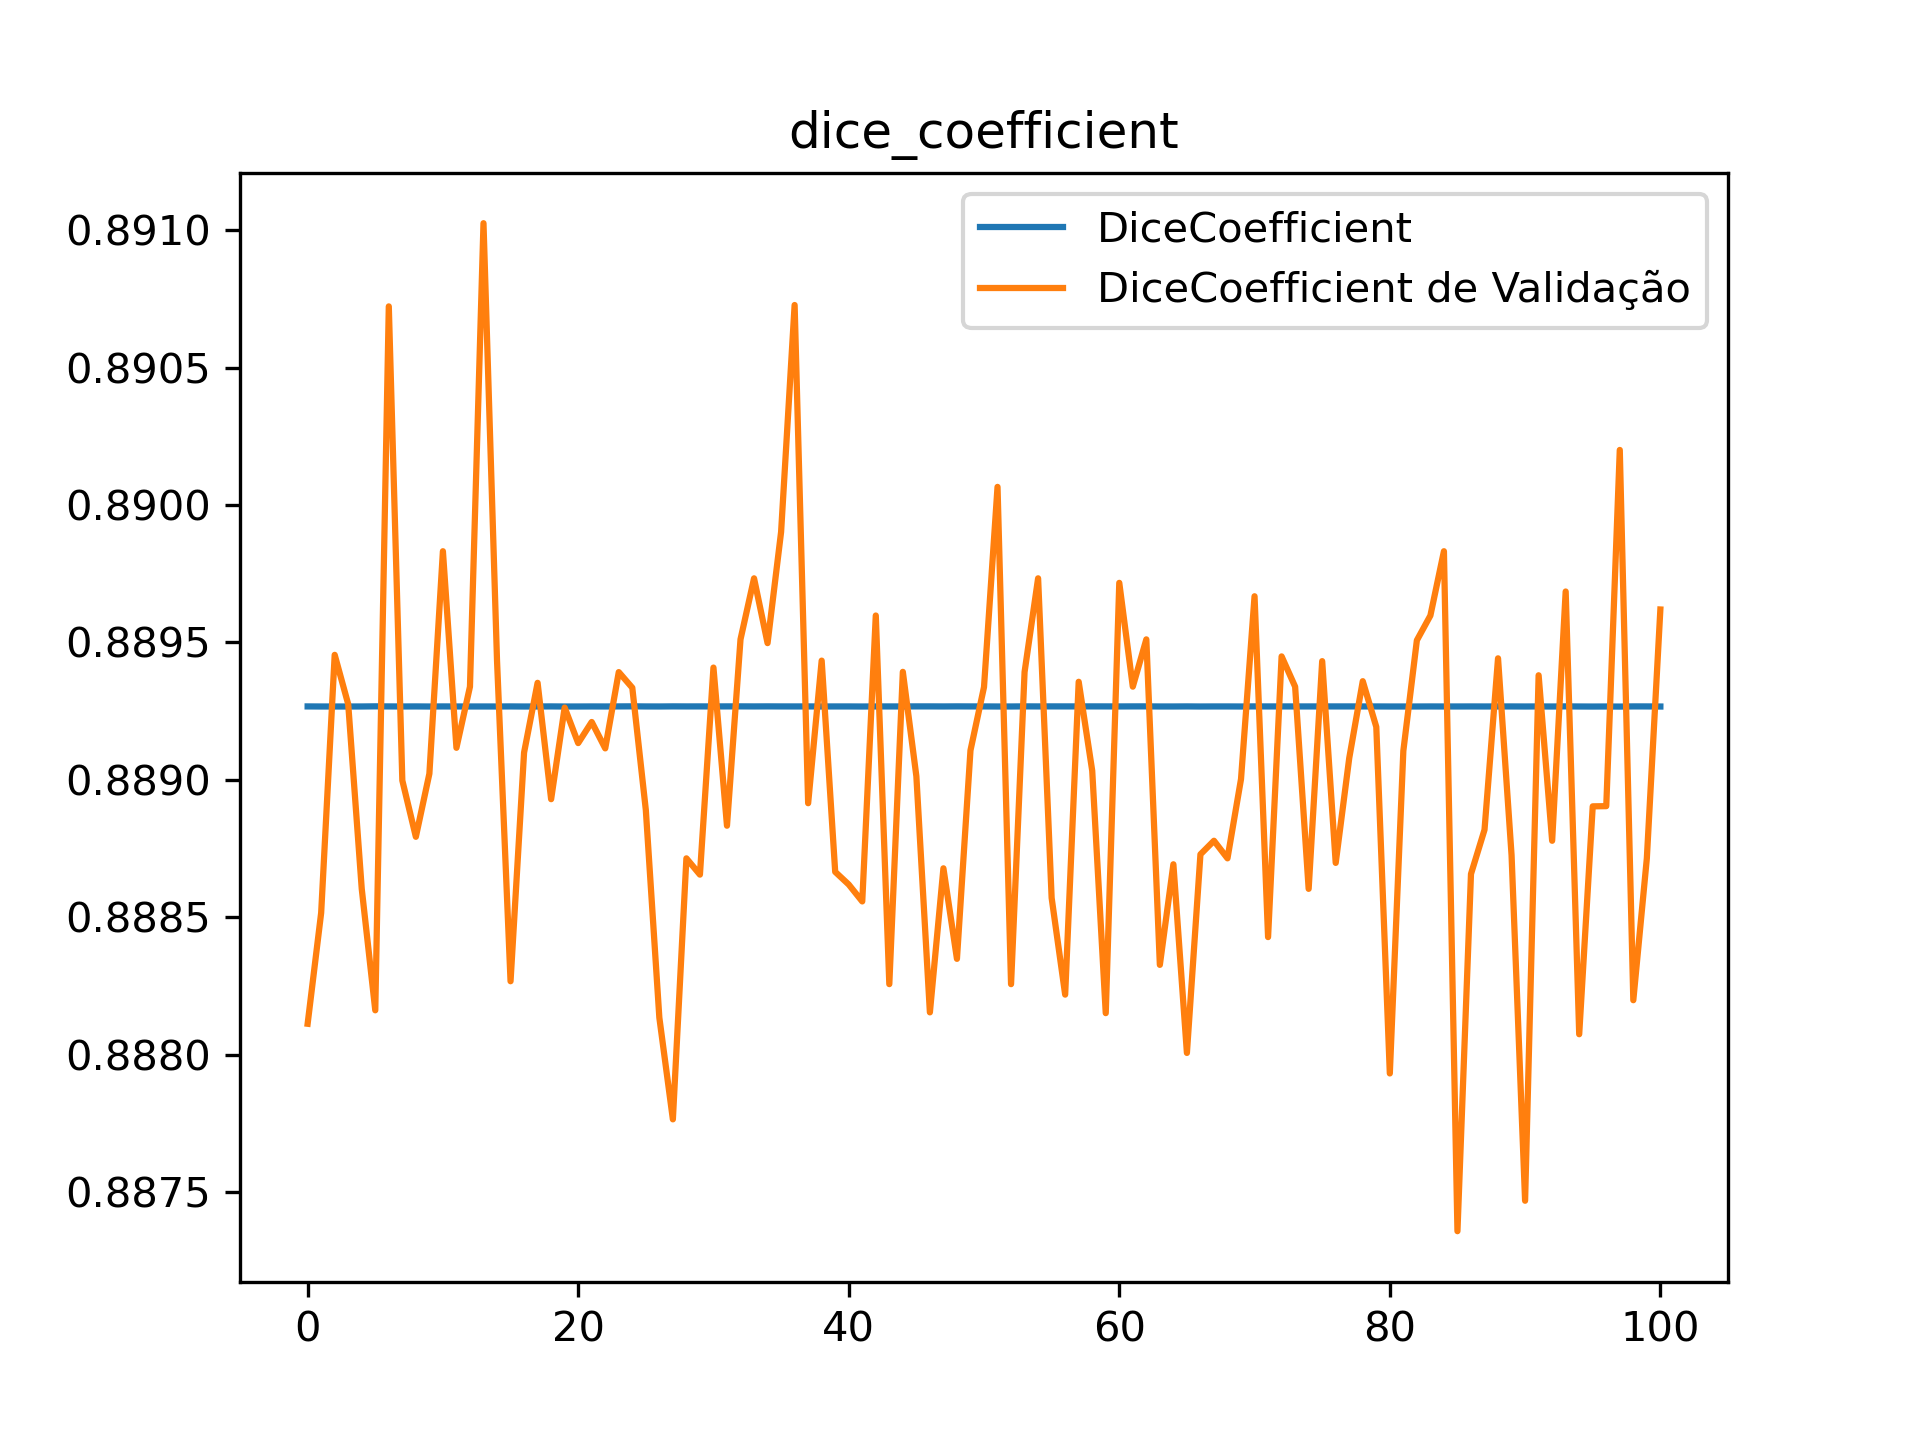
\includegraphics[width=1\linewidth]{recursos/imagens/results/max_unet500_miou_dice_coefficient.png}
         \caption{Dice.}
         \label{results:fig:semantic:metrics3.3}
     \end{subfigure}
     ~
     \begin{subfigure}[t]{0.45\textwidth}
         \centering
         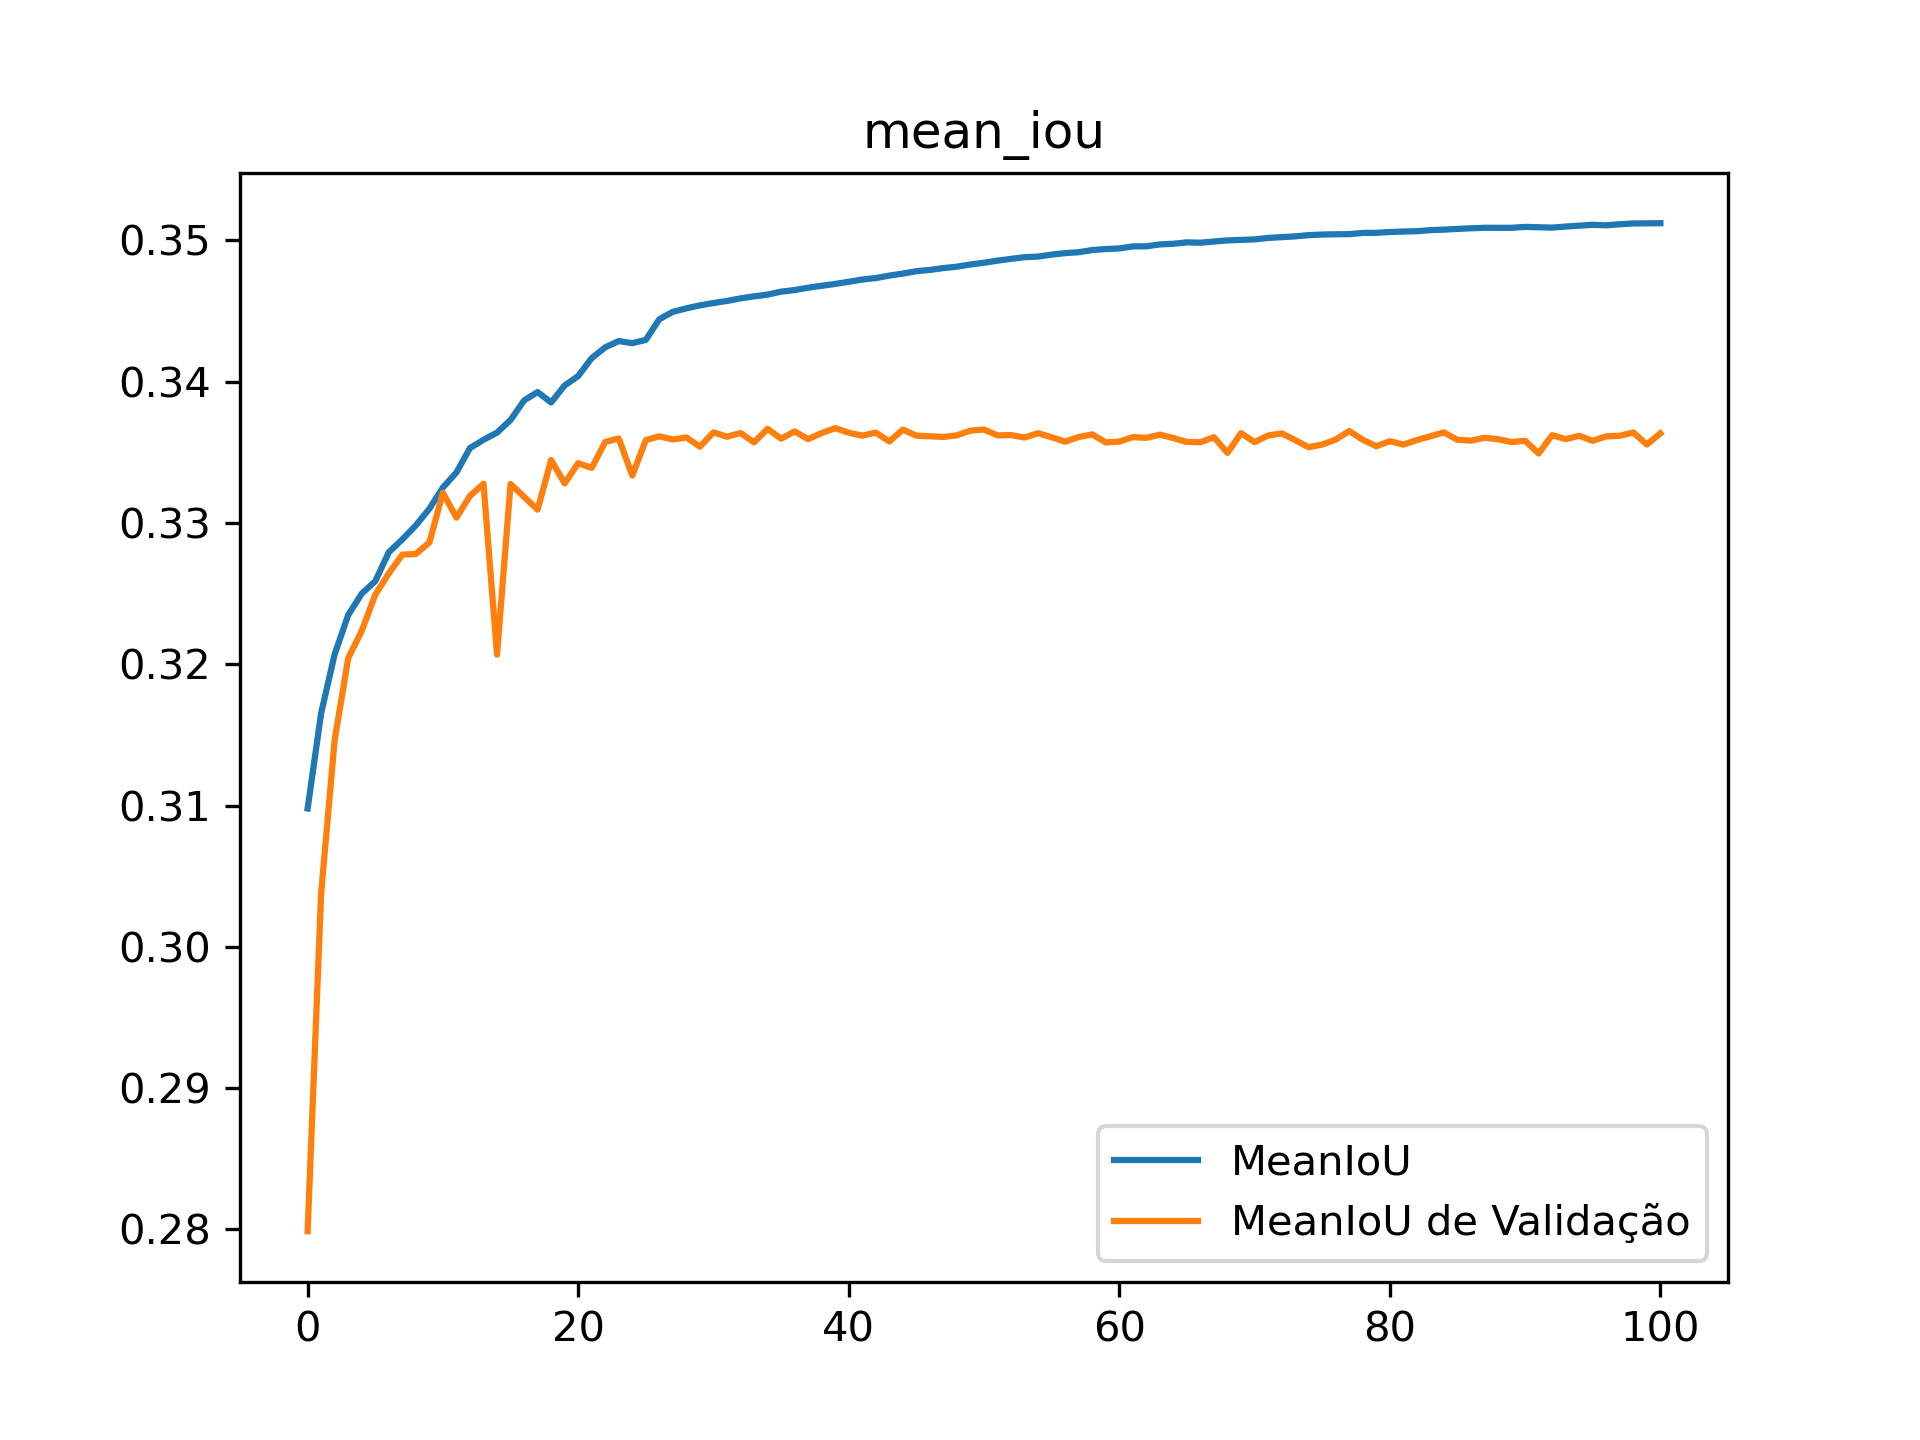
\includegraphics[width=1\linewidth]{recursos/imagens/results/max_unet500_miou_mean_iou.png}
         \caption{mIoU.}
         \label{results:fig:semantic:metrics3.4}
     \end{subfigure}
     
     Fonte: do próprio autor.
\end{figure}

Outro aspecto a se considerar ao analisar as Tabelas \ref{results:semantic:tab:1} e \ref{results:semantic:tab:2} é o tempo de execução durante os processos de treinamento e validação. Notavelmente, os tempos para o método \textit{Max Pooling} são significativamente mais rápidos quando comparado ao BPCAPooling, atribuídos à complexidade do método proposto discutida na Seção \ref{results:class:future}. No entanto, é importante destacar que os modelos atingiram a convergência em um número próximo de épocas, os modelos baseados na métrica de acurácia convergiram em $168$ épocas para BPCAPooling e $172$ épocas para \textit{Max Pooling}. Enquanto, os modelos baseados na métrica mIoU convergiram em $102$ épocas para BPCAPooling e $101$ para \textit{Max Pooling}.

Por fim, ao considerar um nível de significância de $5\%$ para os modelos U-Nets treinados durante $500$ épocas, observa-se que não há diferença significativa nos campos de acurácia, tanto nos conjuntos de teste quanto nos de validação, apresentando p-valores de $0.1479$ e $0.2192$, respectivamente. No entanto, ao analisar os valores de mIoU, embora os p-valores sejam de $0.0678$ e $0.0110$ para teste e validação, respectivamente, indicando ausência de diferença significativa no primeiro caso e uma diferença no segundo caso (considerando um nível de significância de $5\%$), é importante ressaltar que visualmente é desafiador discernir tais diferenças, uma vez que a segmentação apresenta uma semelhança notável, sendo assim maiores detalhes sobre as diferenças serão relatados na Seção \ref{results:semantic:xai}. Os resultados visuais podem ser observados nas Figuras \ref{results:fig:semantic:0} e \ref{results:fig:semantic:1}, correspondendo ao primeiro e segundo caso mencionados, respectivamente.

\begin{figure}[H]
    \centering
   \caption{Imagem de entrada, máscara e saída do modelo U-Net baseado em acurácia, respectivamente.}
    \label{results:fig:semantic:0}
    \begin{subfigure}[t]{0.9\textwidth}
        \centering
        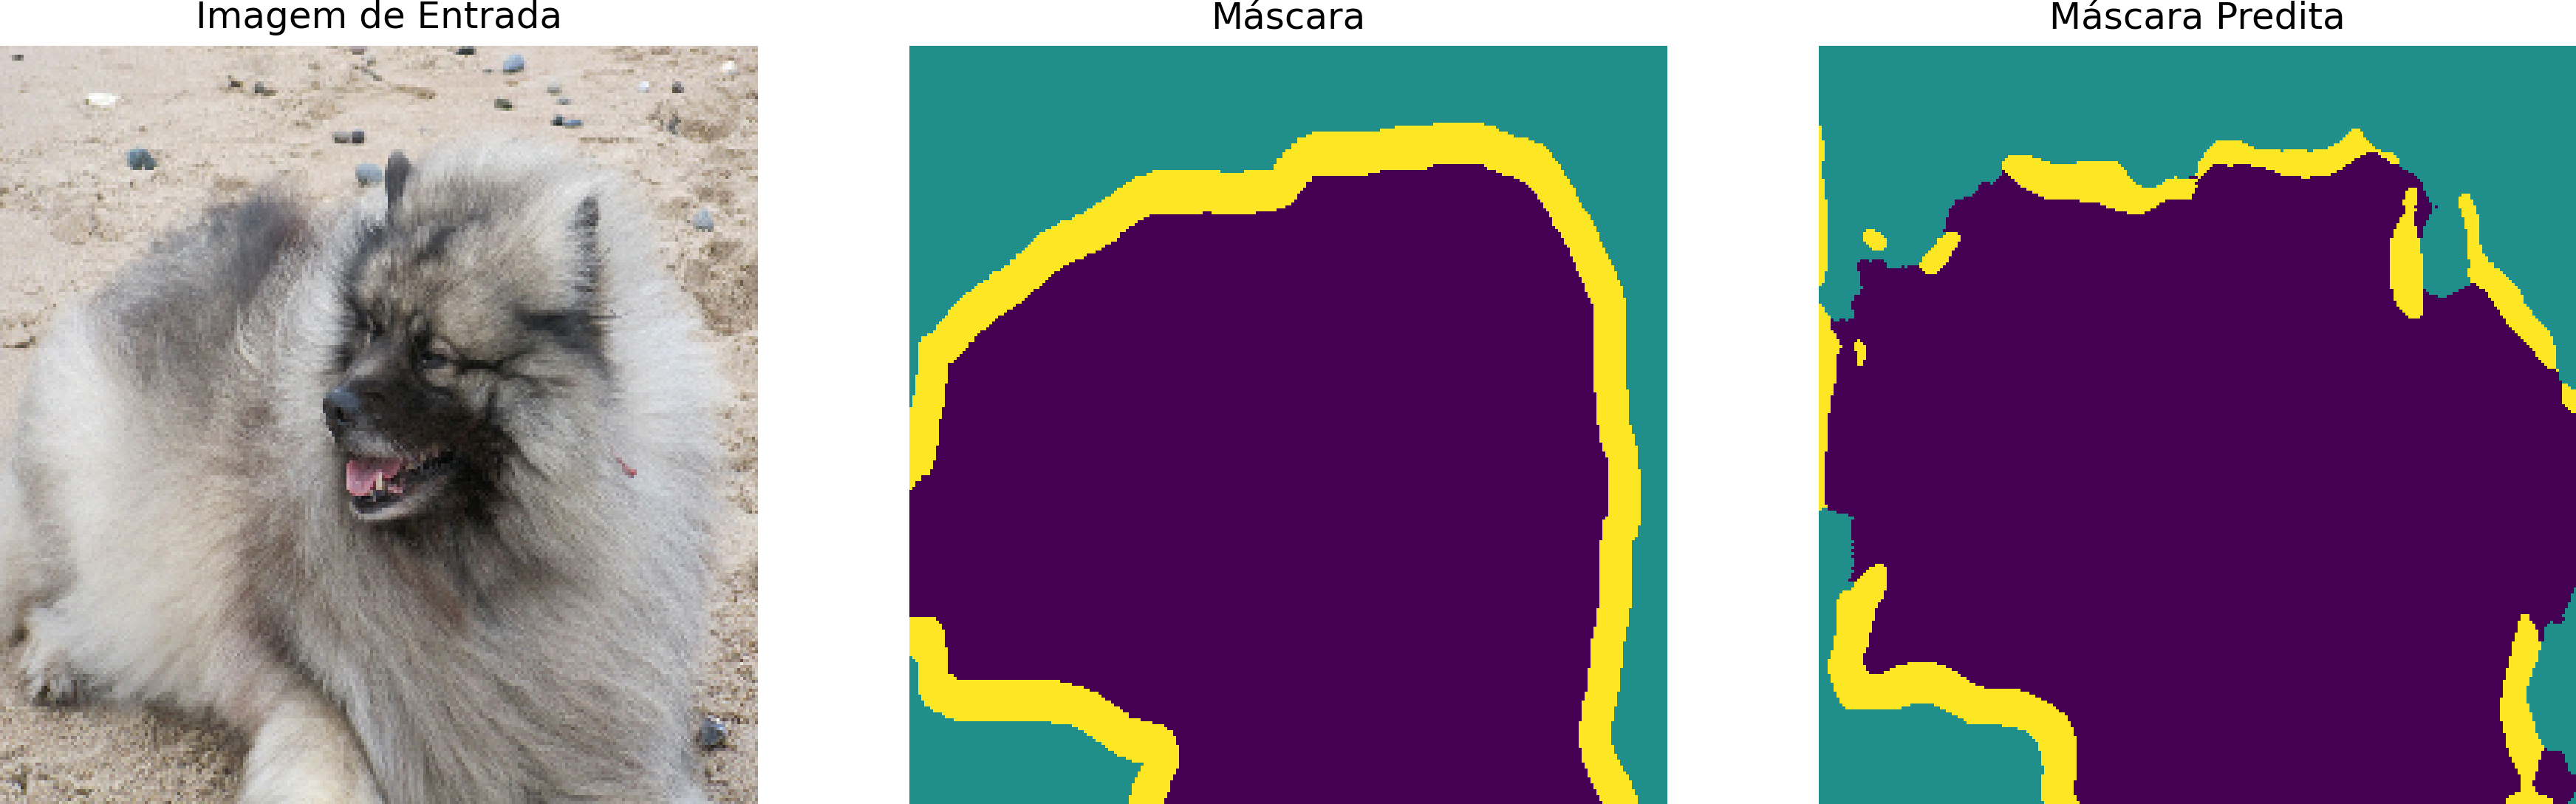
\includegraphics[width=1\linewidth]{recursos/imagens/results/image_0_max_unet_500.png}
        \caption{Modelo com \textit{Max Pooling}.}
        \label{results:fig:semantic:0.1}
    \end{subfigure}%
    ~
    
    \begin{subfigure}[t]{0.9\textwidth}
        \centering
        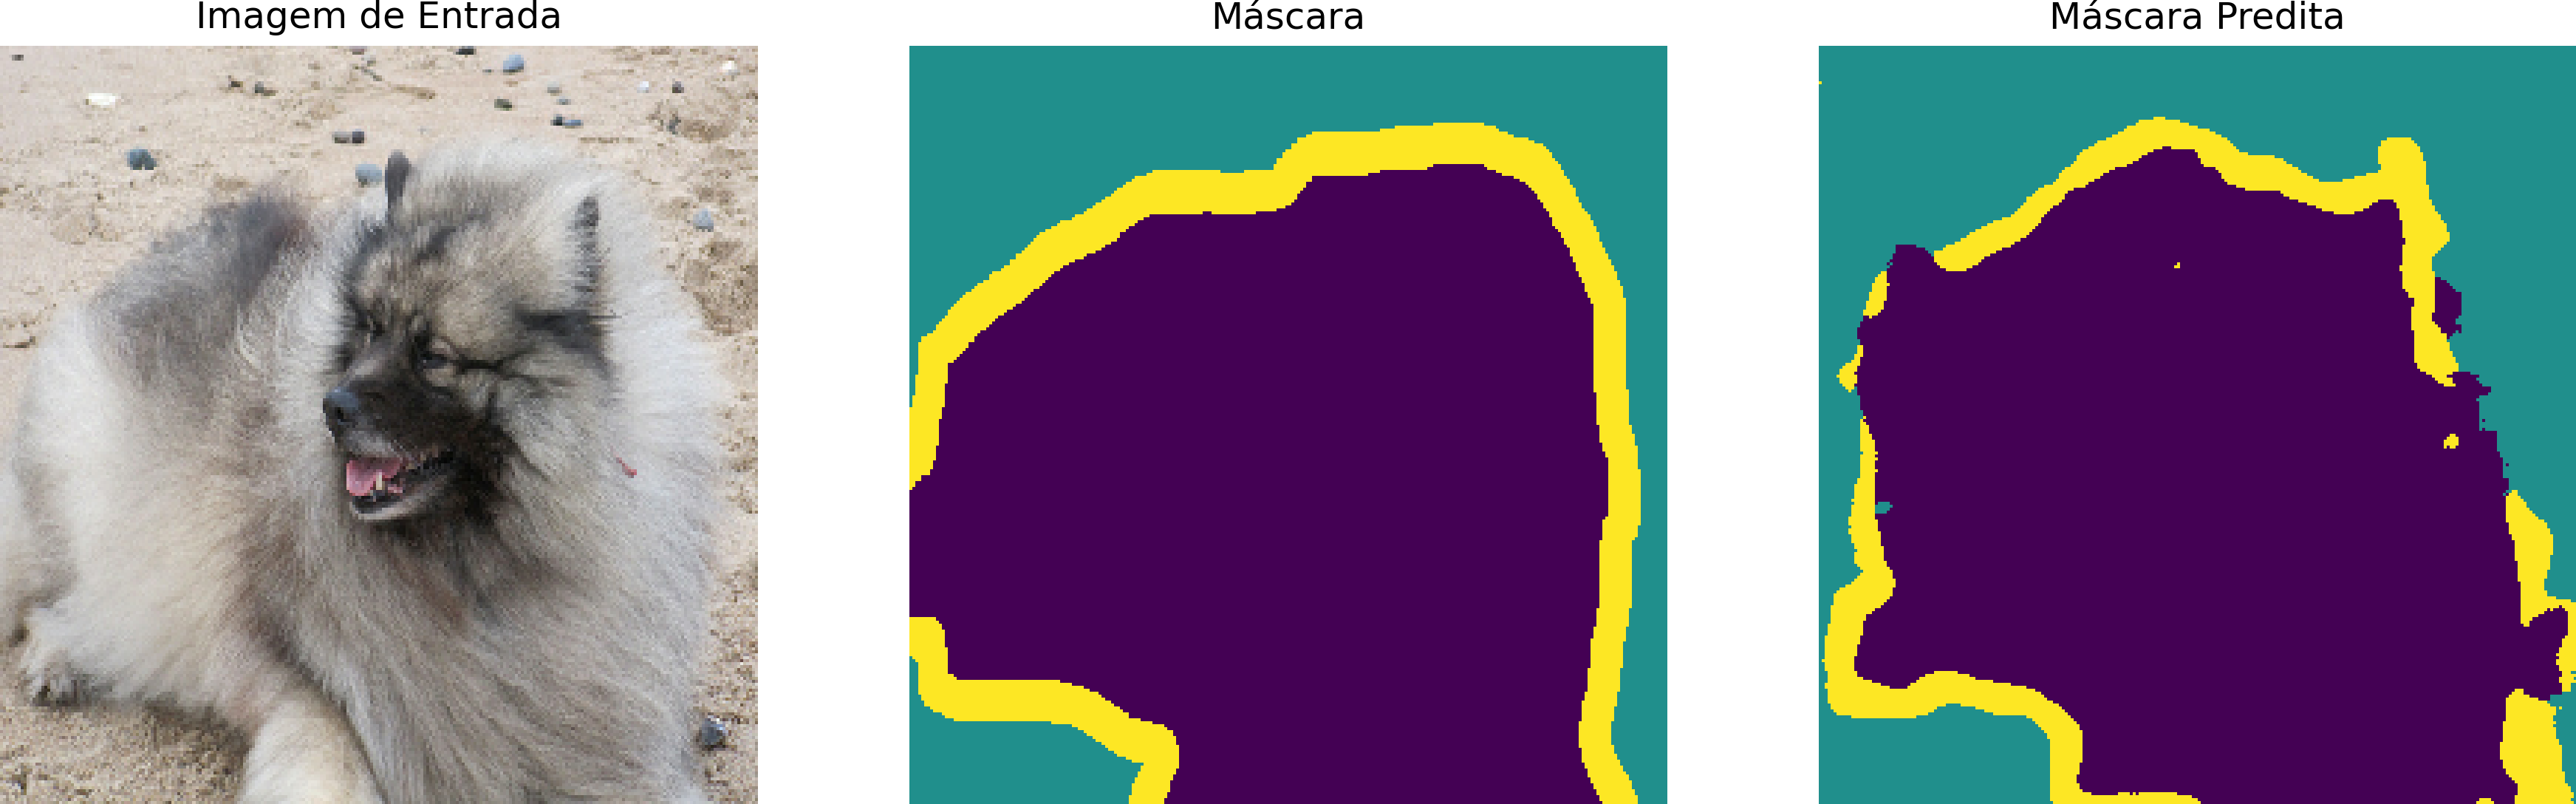
\includegraphics[width=1\linewidth]{recursos/imagens/results/image_0_bpca_unet_500.png}
        \caption{Modelo com BPCAPooling.}
        \label{results:fig:semantic:0.2}
    \end{subfigure}%

    Fonte: do próprio autor.
\end{figure}


\begin{figure}[H]
    \centering
   \caption{Imagem de entrada, máscara e saída do modelo U-Net baseado em mIoU, respectivamente.}
    \label{results:fig:semantic:1}
    \begin{subfigure}[t]{0.9\textwidth}
        \centering
        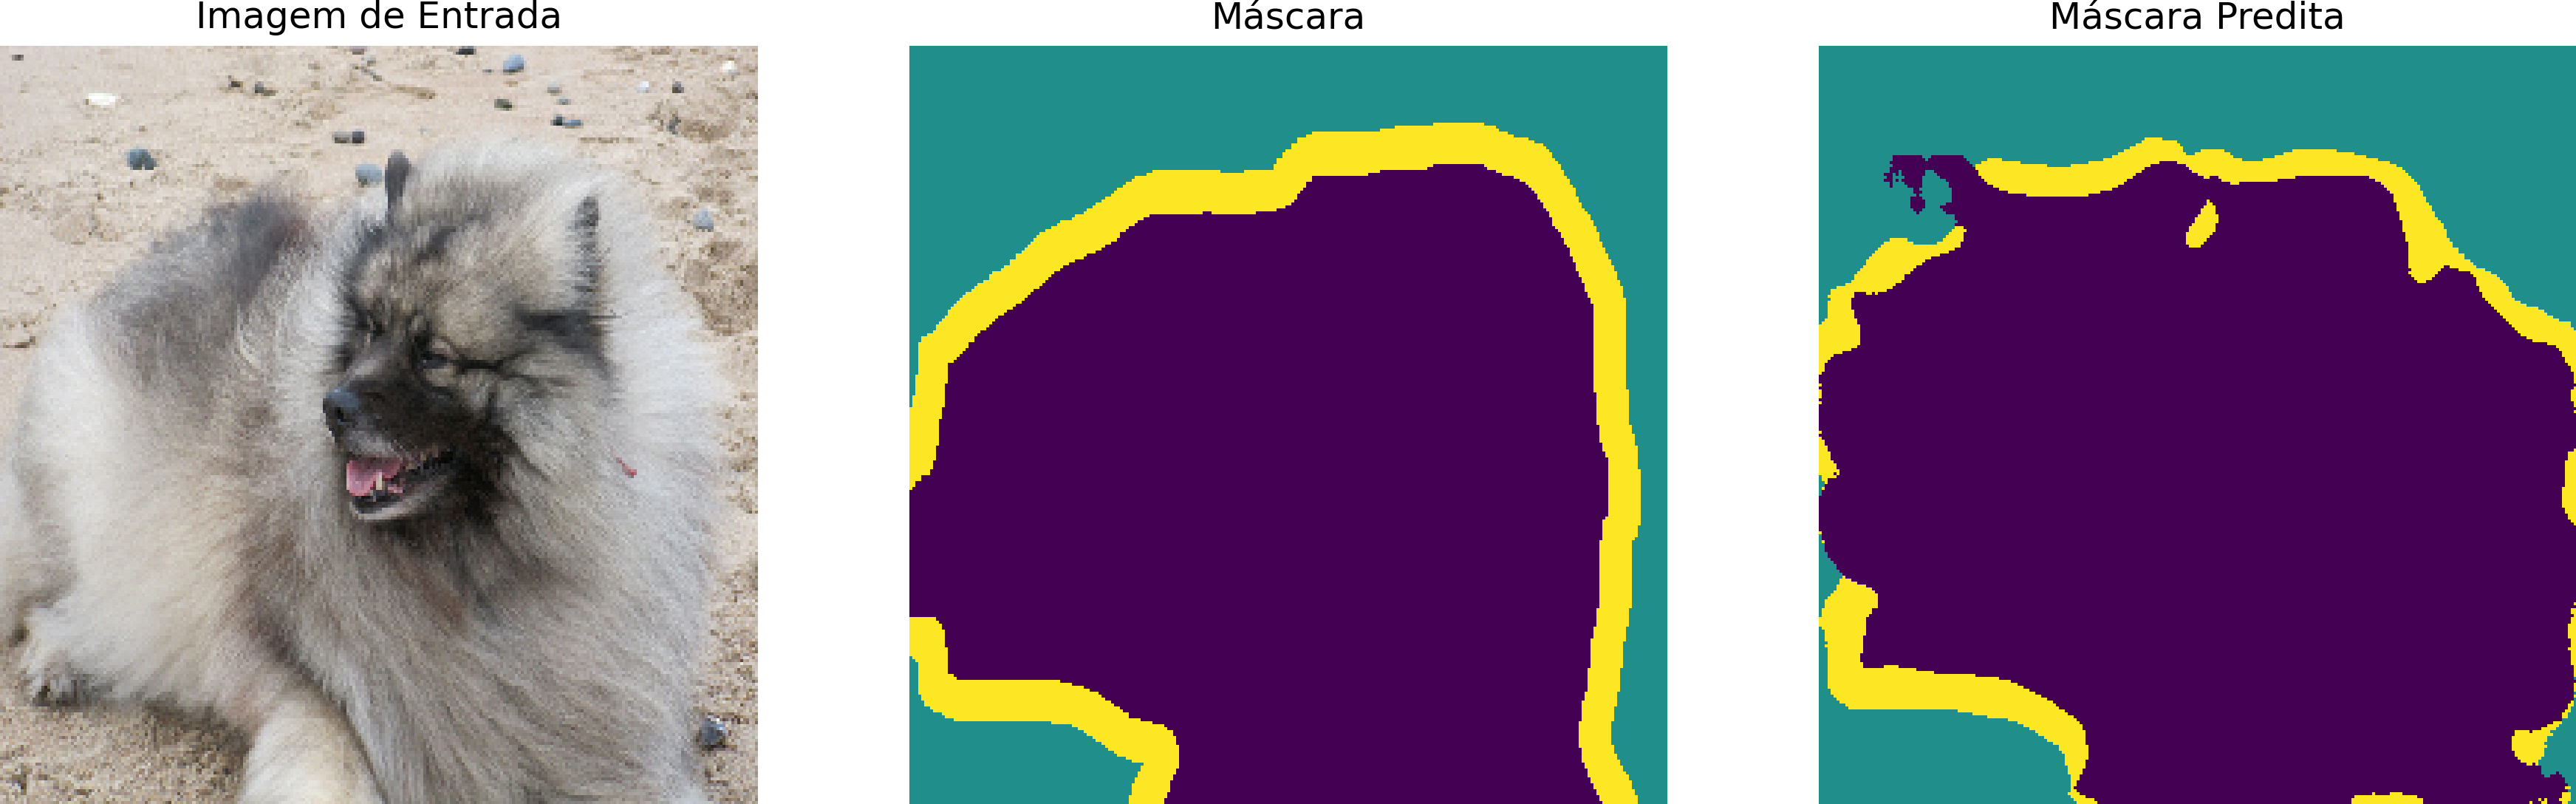
\includegraphics[width=1\linewidth]{recursos/imagens/results/image_0_max_unet_miou.png}
        \caption{Modelo com \textit{Max Pooling}.}
        \label{results:fig:semantic:1.1}
    \end{subfigure}%
    ~
    
    \begin{subfigure}[t]{1\textwidth}
        \centering
        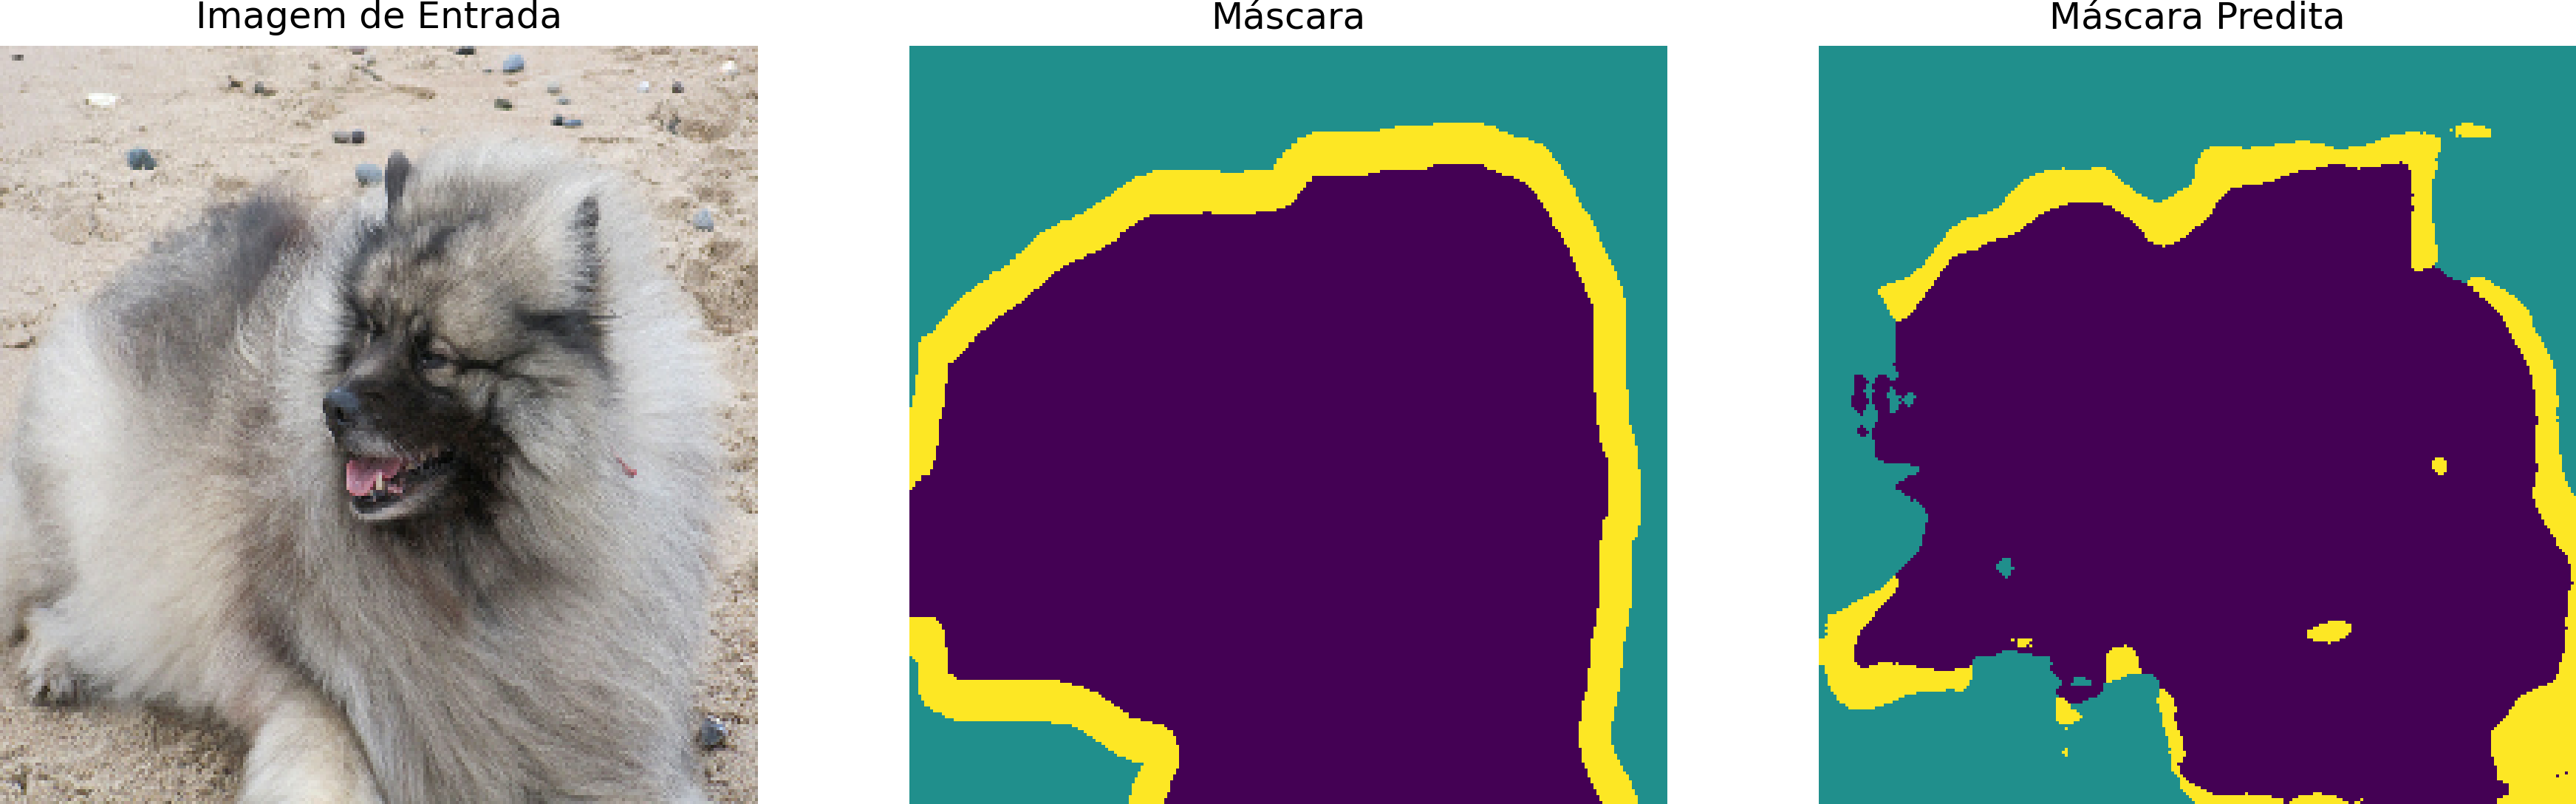
\includegraphics[width=0.9\linewidth]{recursos/imagens/results/image_0_bpca_unet_miou.png}
        \caption{Modelo com BPCAPooling.}
        \label{results:fig:semantic:1.2}
    \end{subfigure}%

    Fonte: do próprio autor.
\end{figure}

Três representações das máscaras previstas sobrepondo a imagem de entrada são exibidas para cada um dos modelos nas Figuras \ref{results:fig:semantic:2}, \ref{results:fig:semantic:3}, \ref{results:fig:semantic:4} e \ref{results:fig:semantic:5}. Observa-se que a aplicação da métrica mIoU se mostra mais eficaz quando comparada à acurácia. Além disso, o método BPCAPooling enfatiza mais os contornos em comparação com o método \textit{Max Pooling}, que aparentemente enfatiza mais os \textit{pets}, tendo que para ambos os métodos o fundo possui a mesma eficacia de segmentação.

\begin{figure}[H]
    \centering
    \caption{Exemplos segmentados a partir de U-Net com \textit{Max Pooling} e 500 épocas no conjunto de dados \textit{Oxford-IIIT Pets} baseada em mIoU.}
    \label{results:fig:semantic:2}
     \begin{subfigure}[t]{0.32\textwidth}
         \centering
         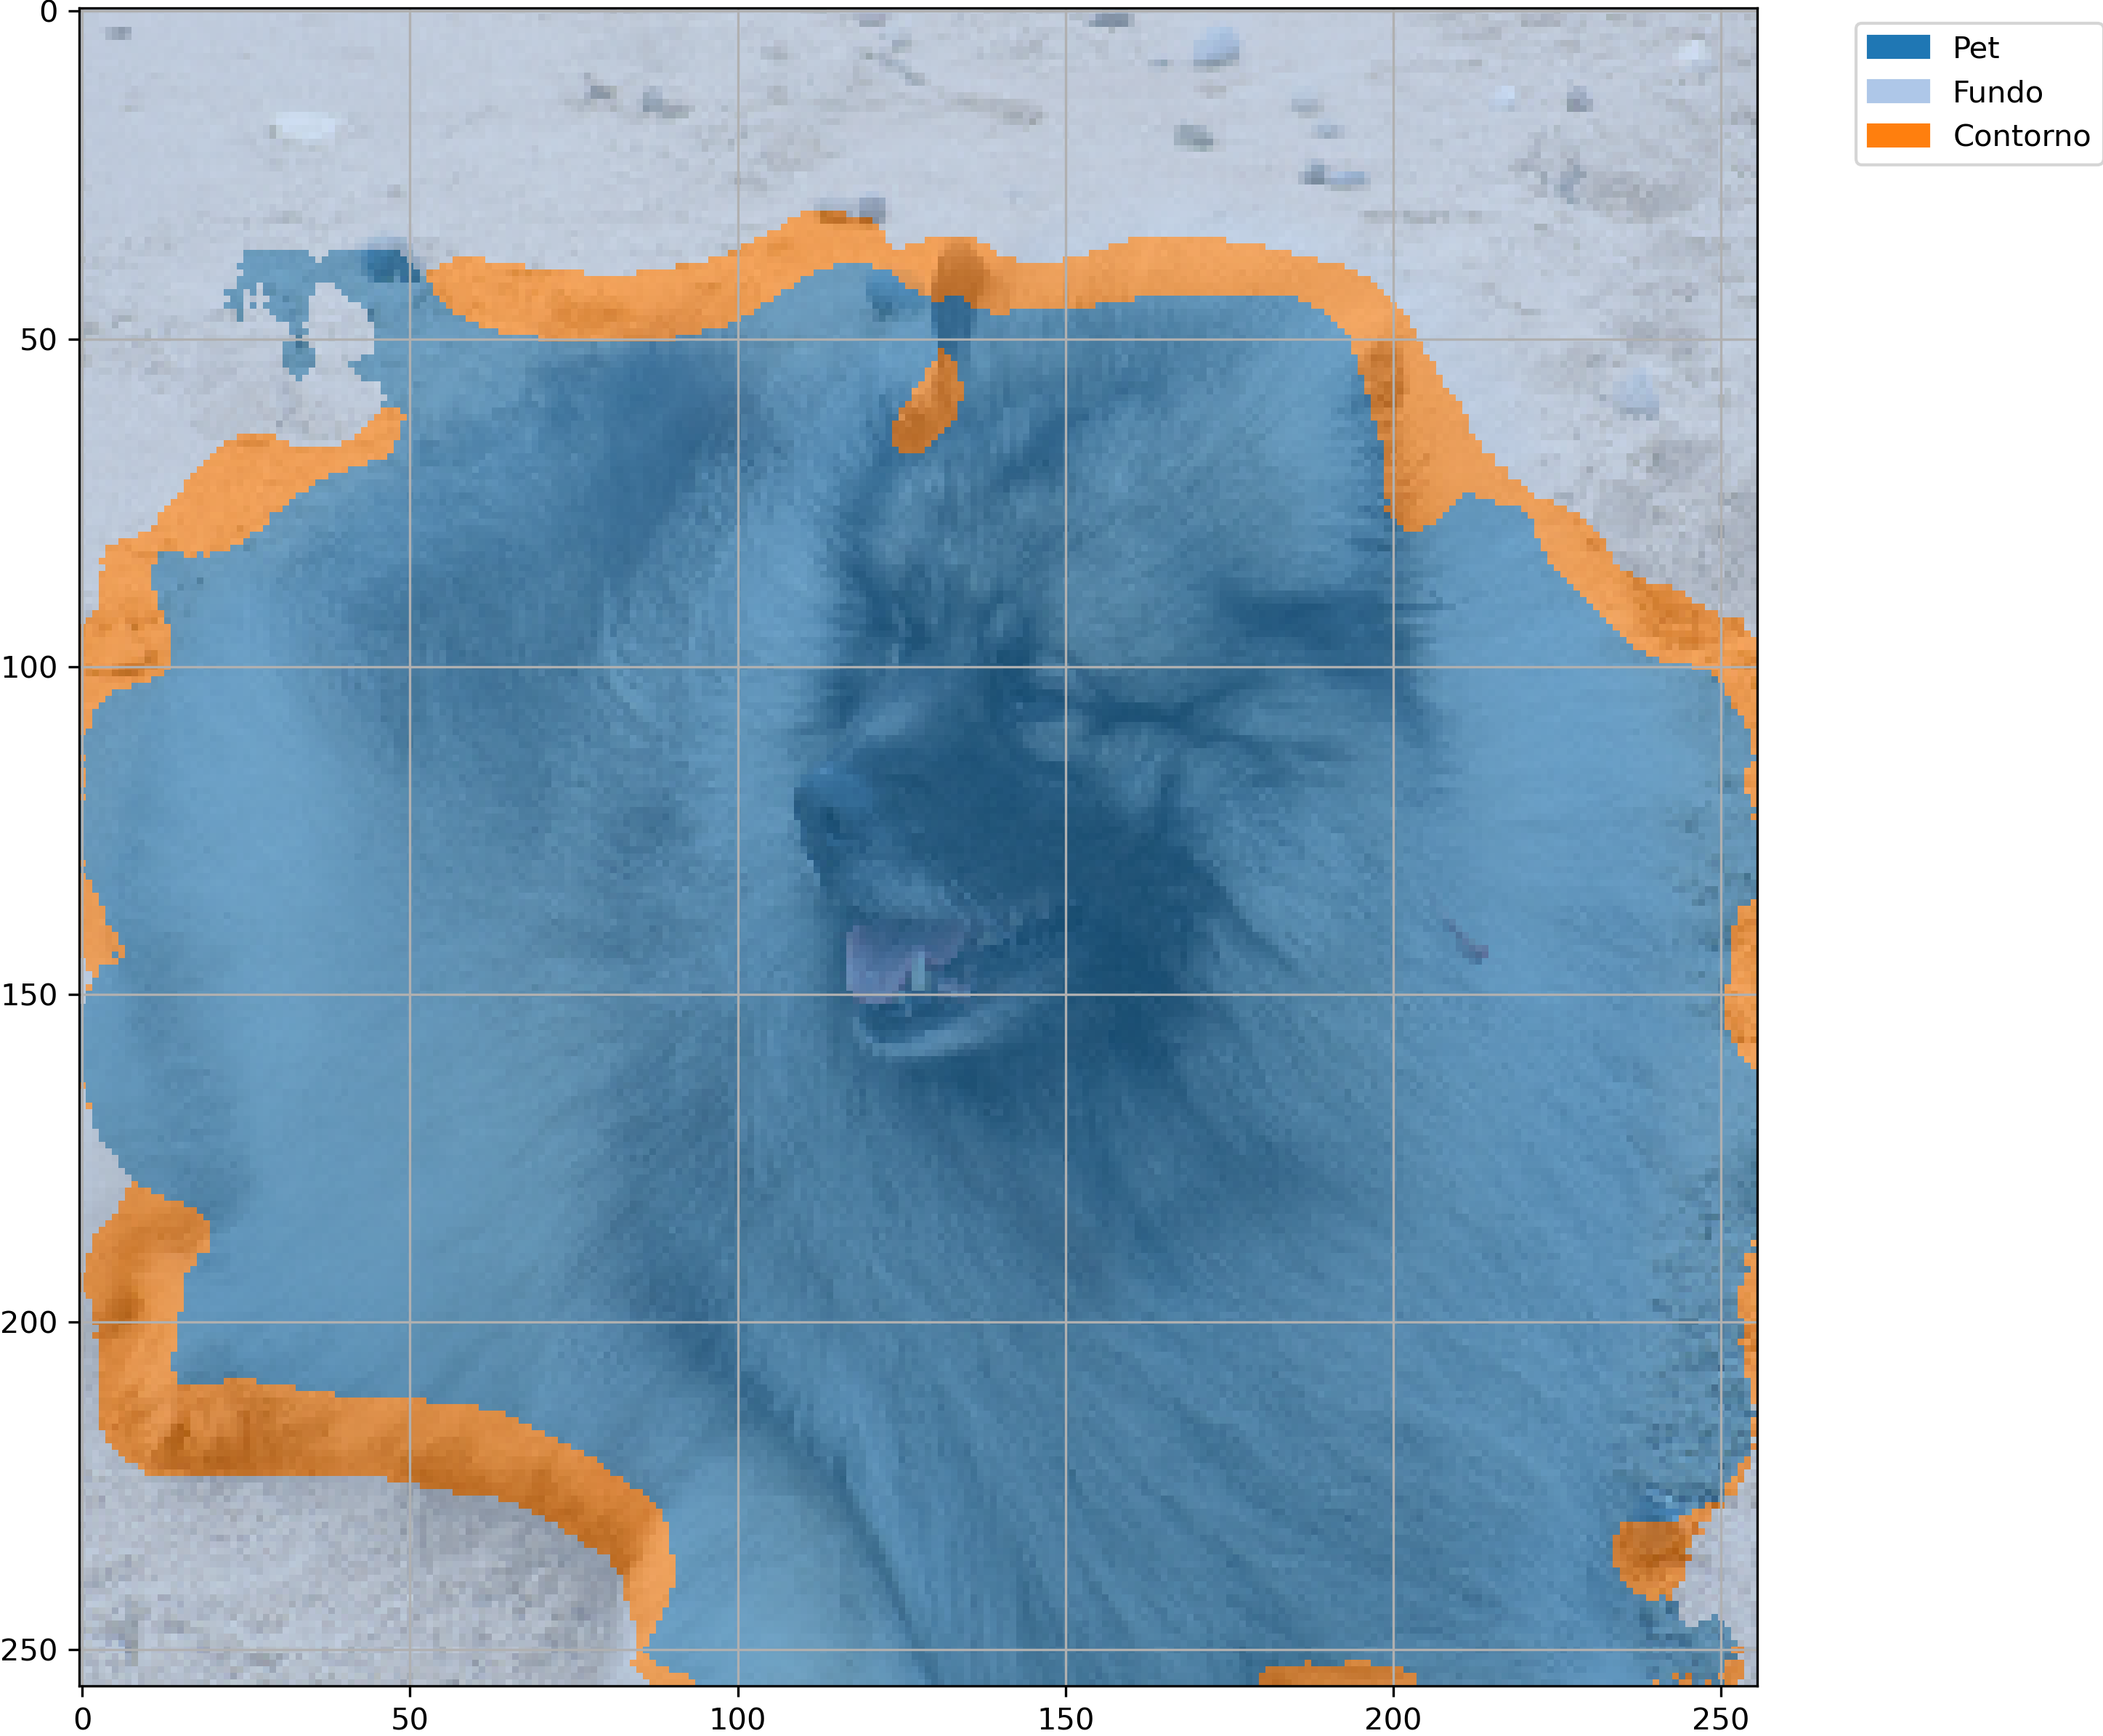
\includegraphics[width=1\linewidth]{recursos/imagens/results/max_miou_unet500_image_0_overlayed_segmentation.png}
         \label{results:fig:semantic:2.1}
     \end{subfigure}%
     ~ 
     \begin{subfigure}[t]{0.32\textwidth}
         \centering
         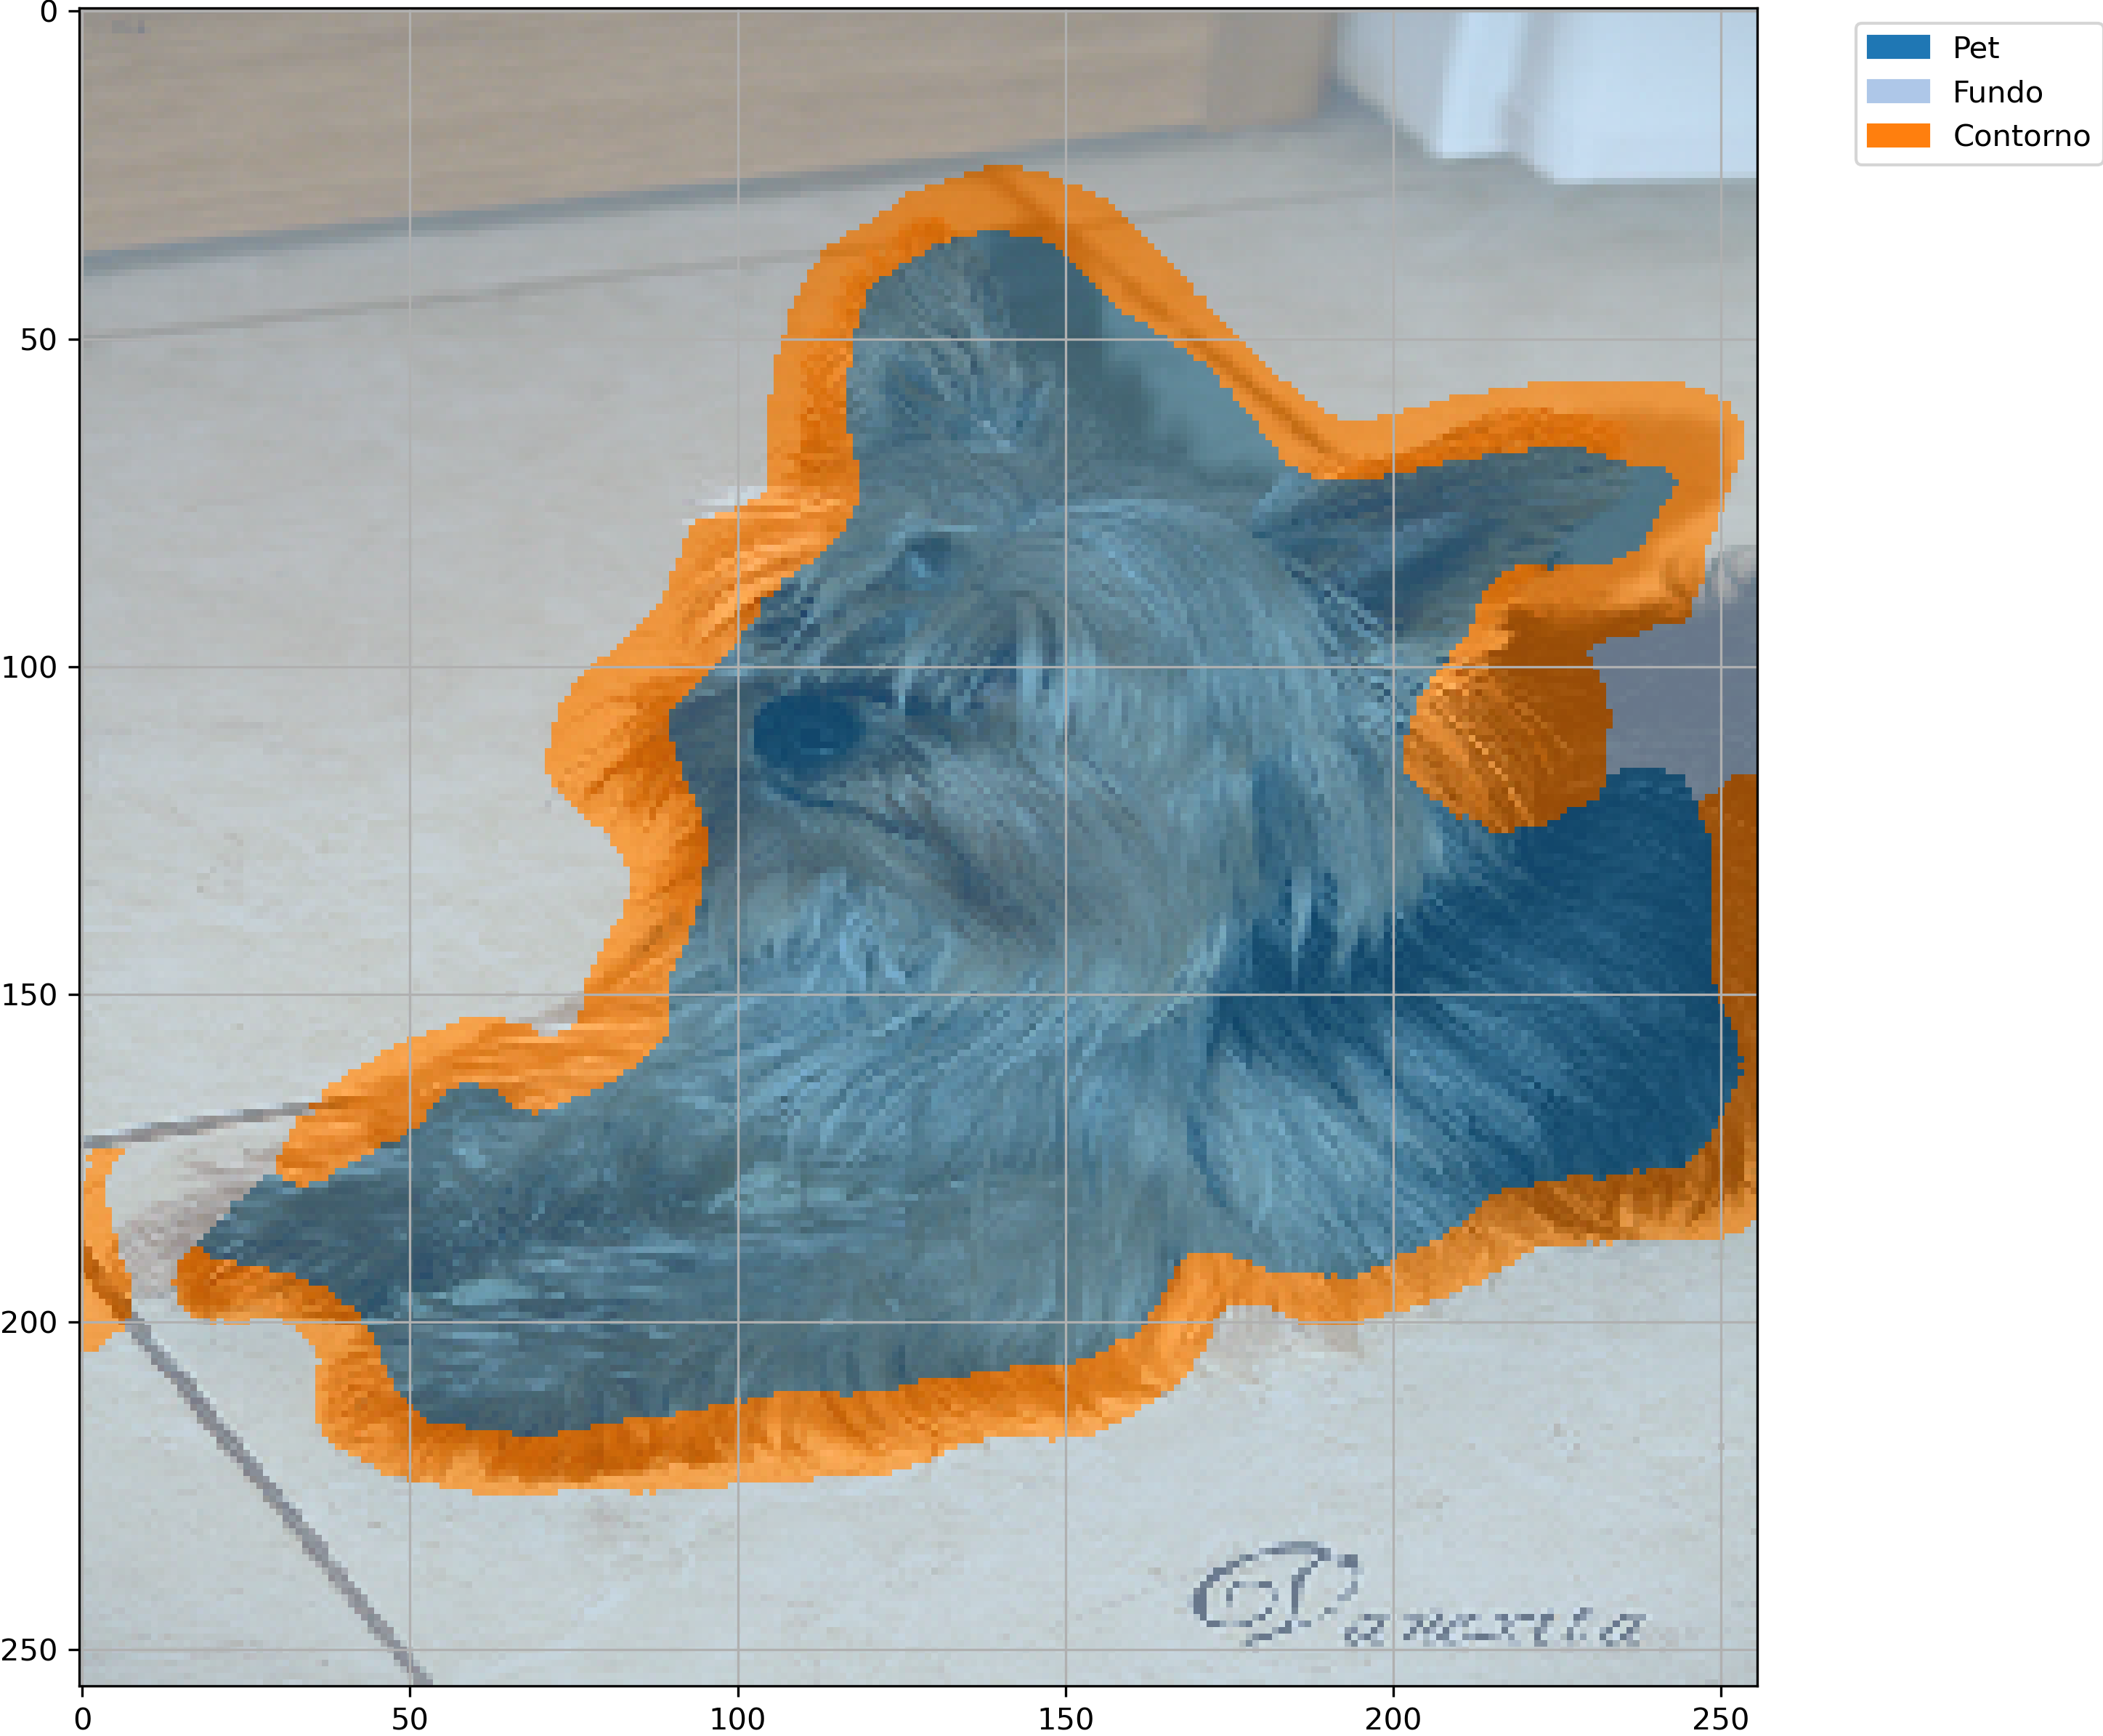
\includegraphics[width=1\linewidth]{recursos/imagens/results/max_miou_unet500_image_1_overlayed_segmentation.png}
         \label{results:fig:semantic:2.2}
     \end{subfigure}%
     ~ 
    \begin{subfigure}[t]{0.32\textwidth}
         \centering
         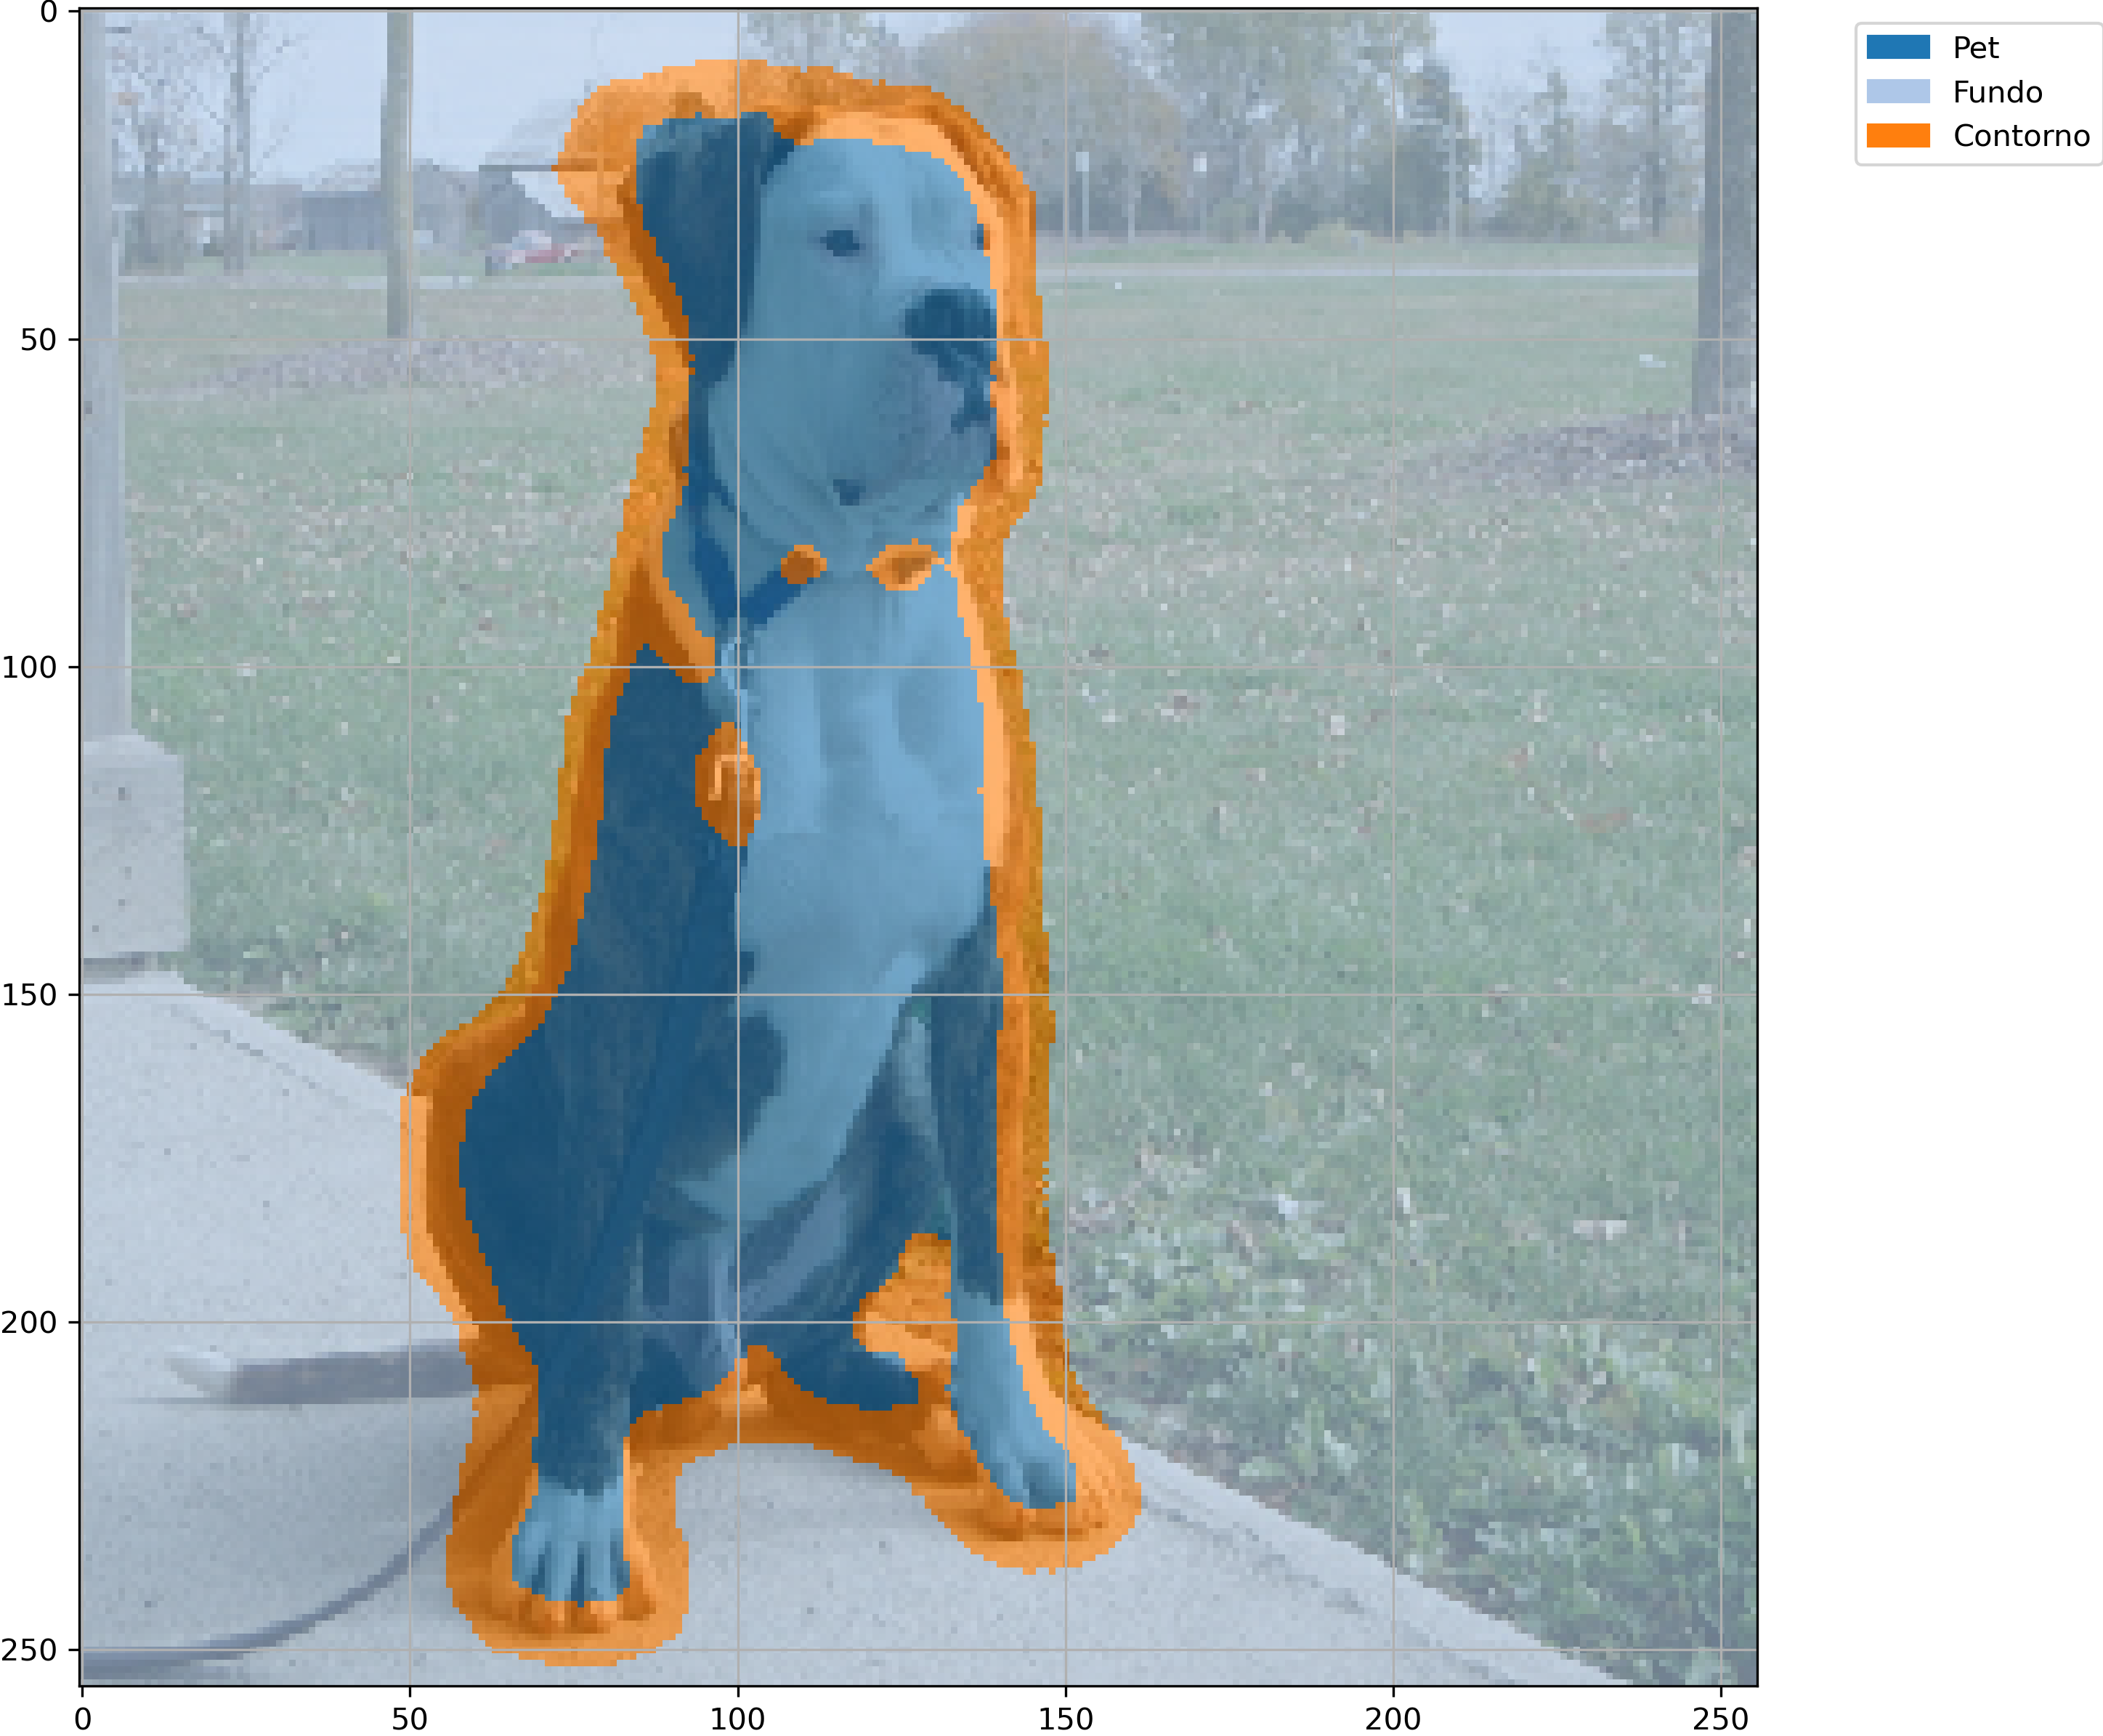
\includegraphics[width=1\linewidth]{recursos/imagens/results/max_miou_unet500_image_2_overlayed_segmentation.png}
         \label{results:fig:semantic:2.2}
     \end{subfigure}%

    Fonte: do próprio autor.
\end{figure}

\begin{figure}[H]
    \centering
    \caption{Exemplos segmentados a partir de U-Net com BPCAPooling e 500 épocas no conjunto de dados \textit{Oxford-IIIT Pets} baseada em mIoU.}
    \label{results:fig:semantic:3}
     \begin{subfigure}[t]{0.32\textwidth}
         \centering
         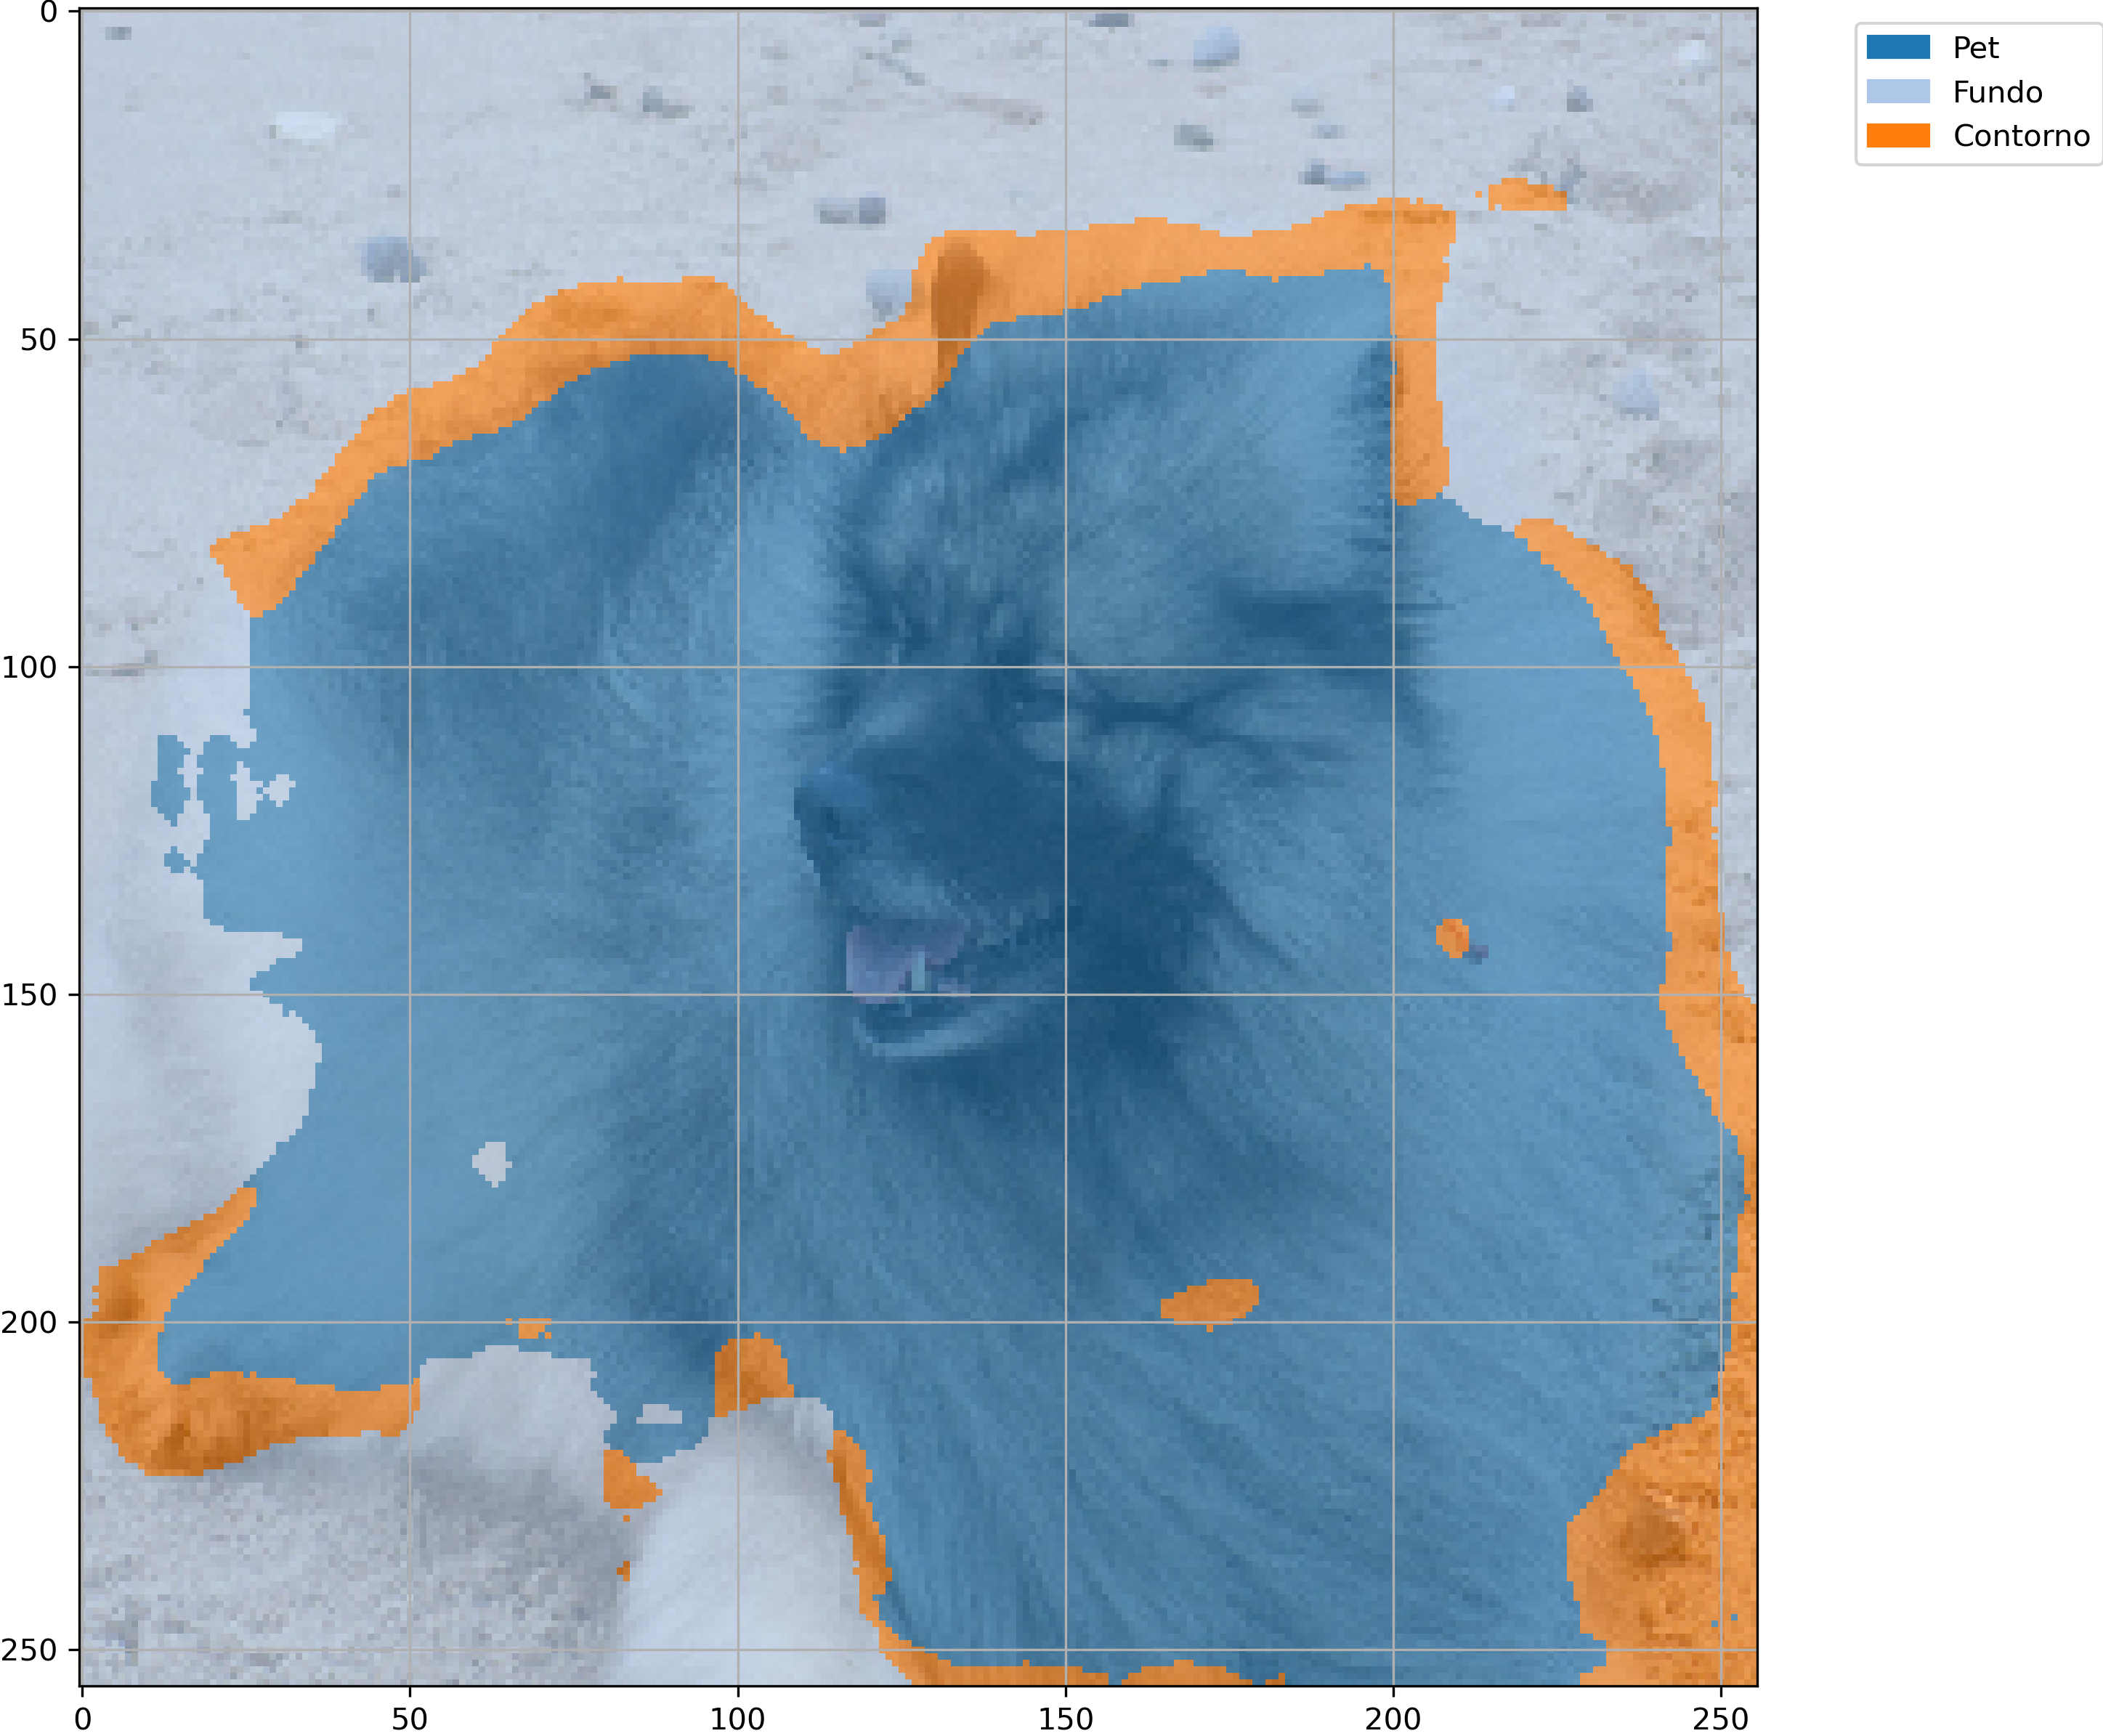
\includegraphics[width=1\linewidth]{recursos/imagens/results/bpca_miou_unet500_image_0_overlayed_segmentation.png}
         \label{results:fig:semantic:3.1}
     \end{subfigure}%
     ~ 
     \begin{subfigure}[t]{0.32\textwidth}
         \centering
         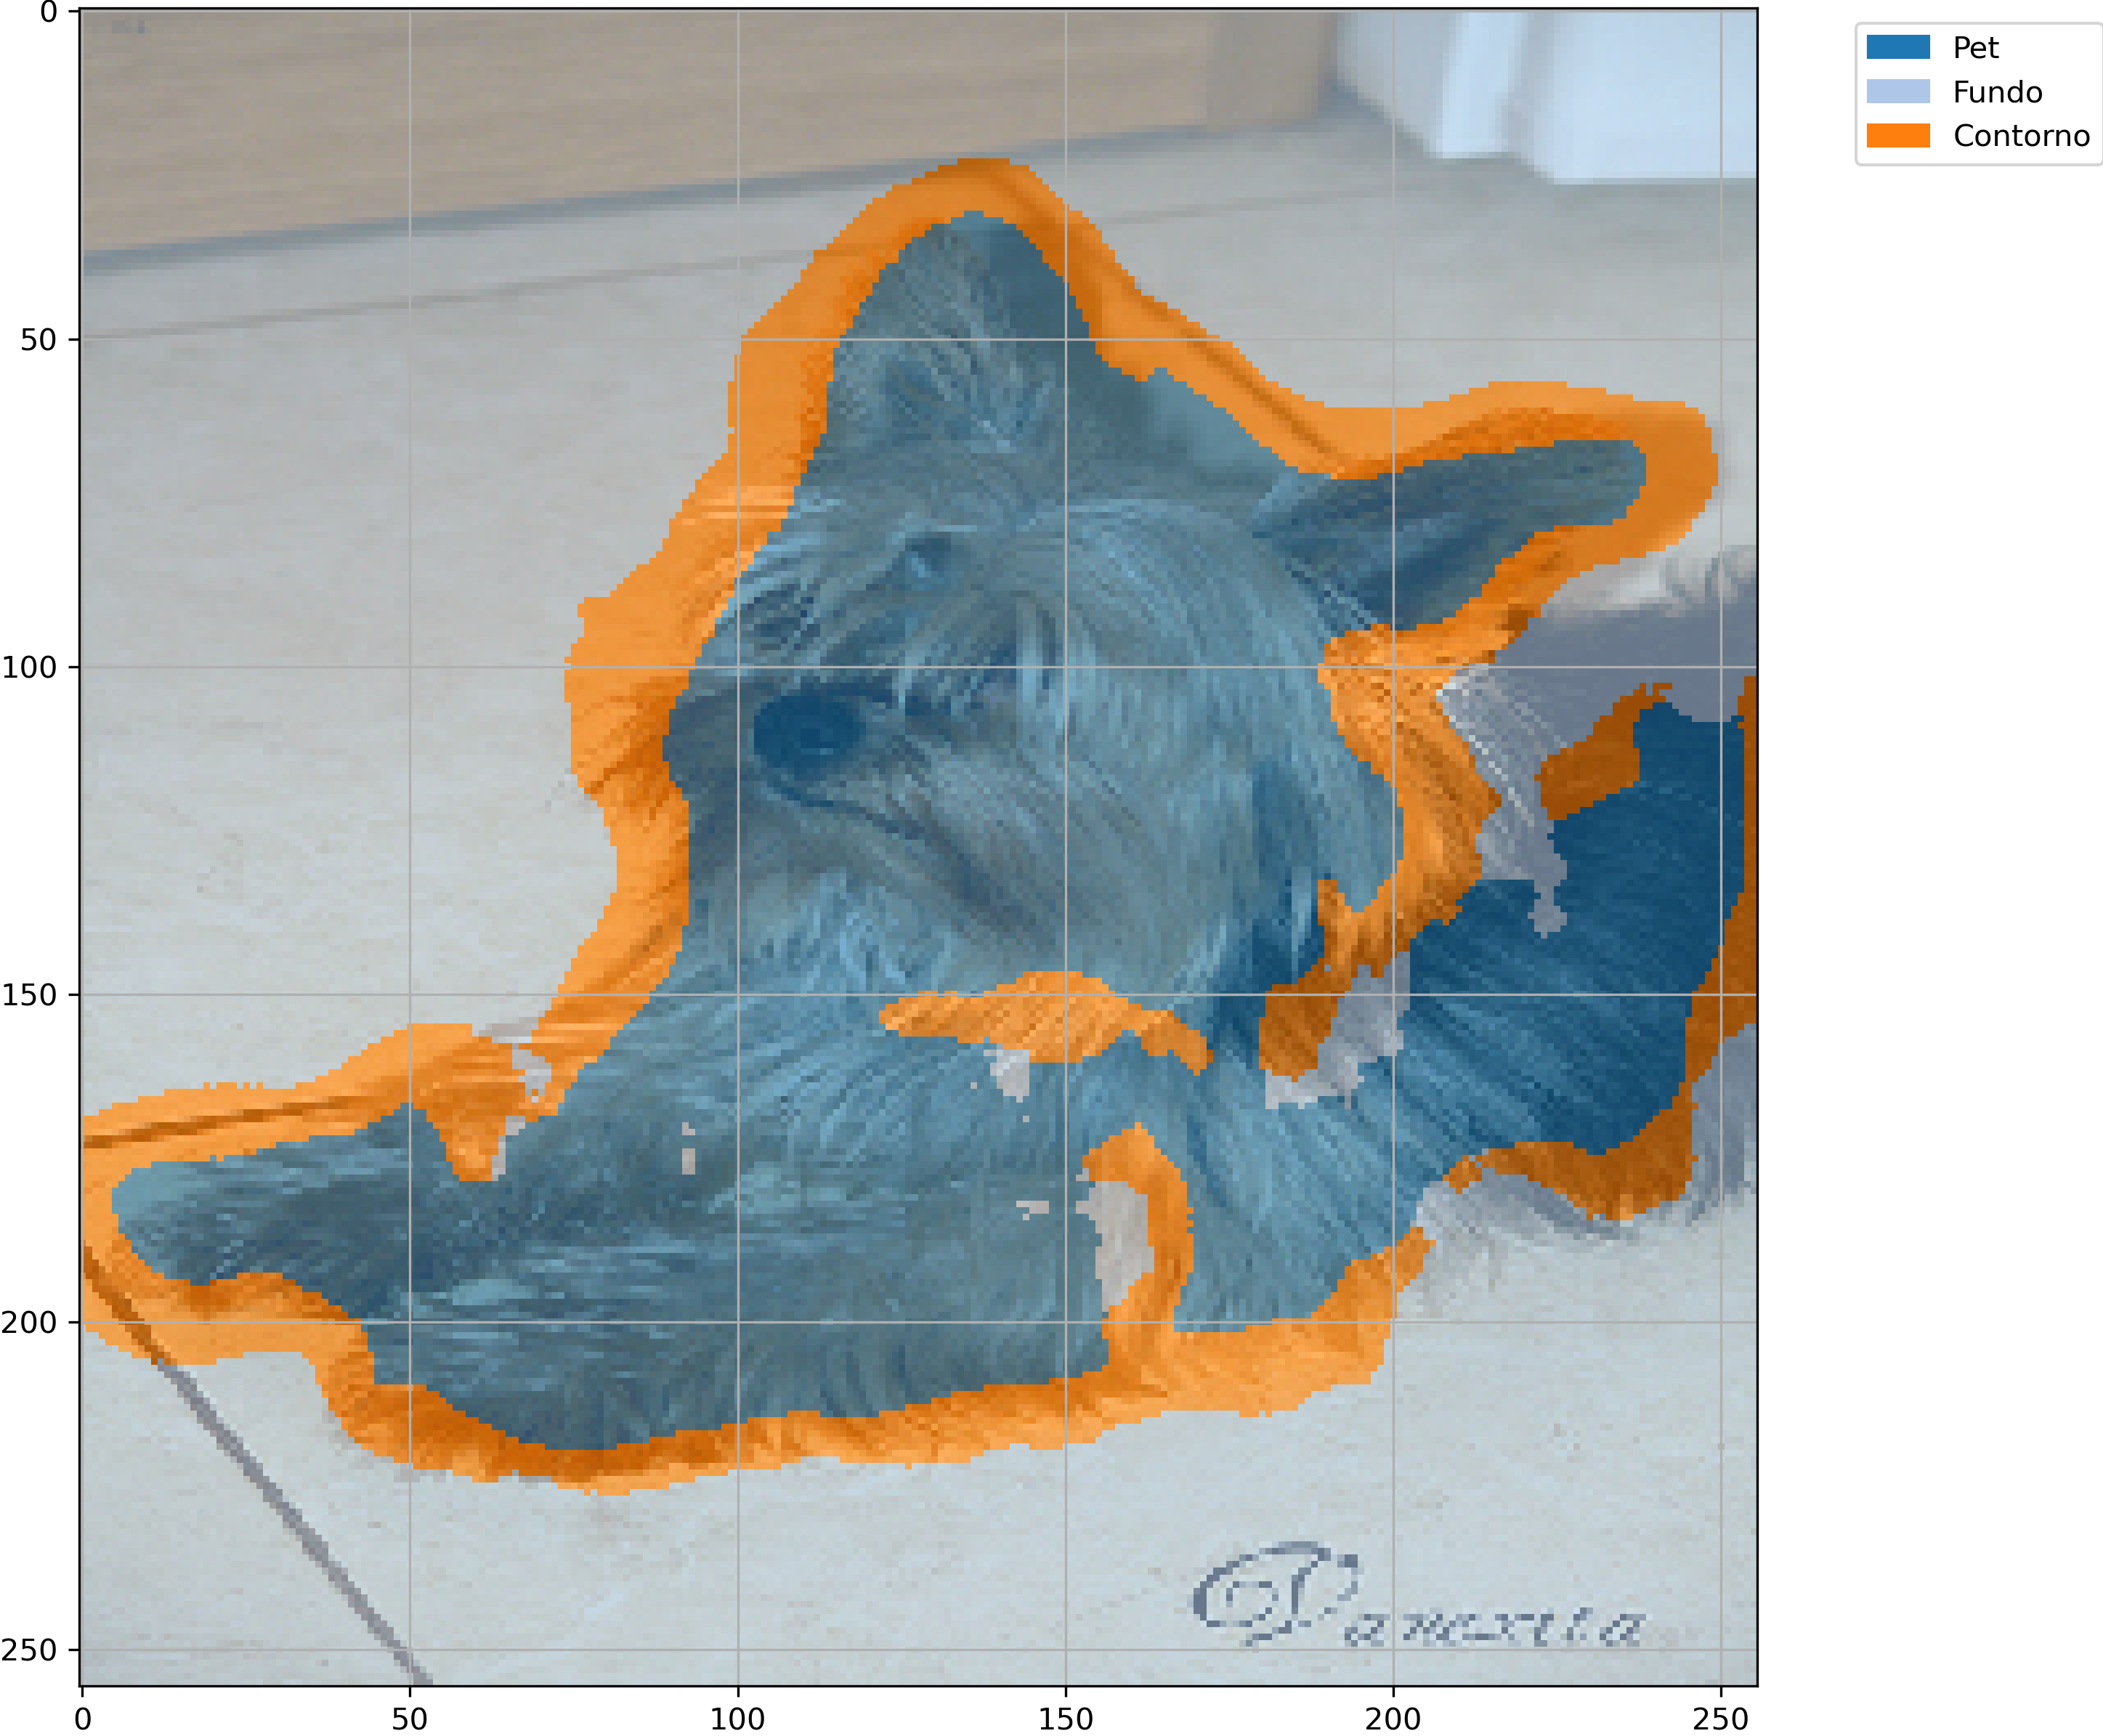
\includegraphics[width=1\linewidth]{recursos/imagens/results/bpca_miou_unet500_image_1_overlayed_segmentation.png}
         \label{results:fig:semantic:3.2}
     \end{subfigure}%
     ~ 
    \begin{subfigure}[t]{0.32\textwidth}
         \centering
         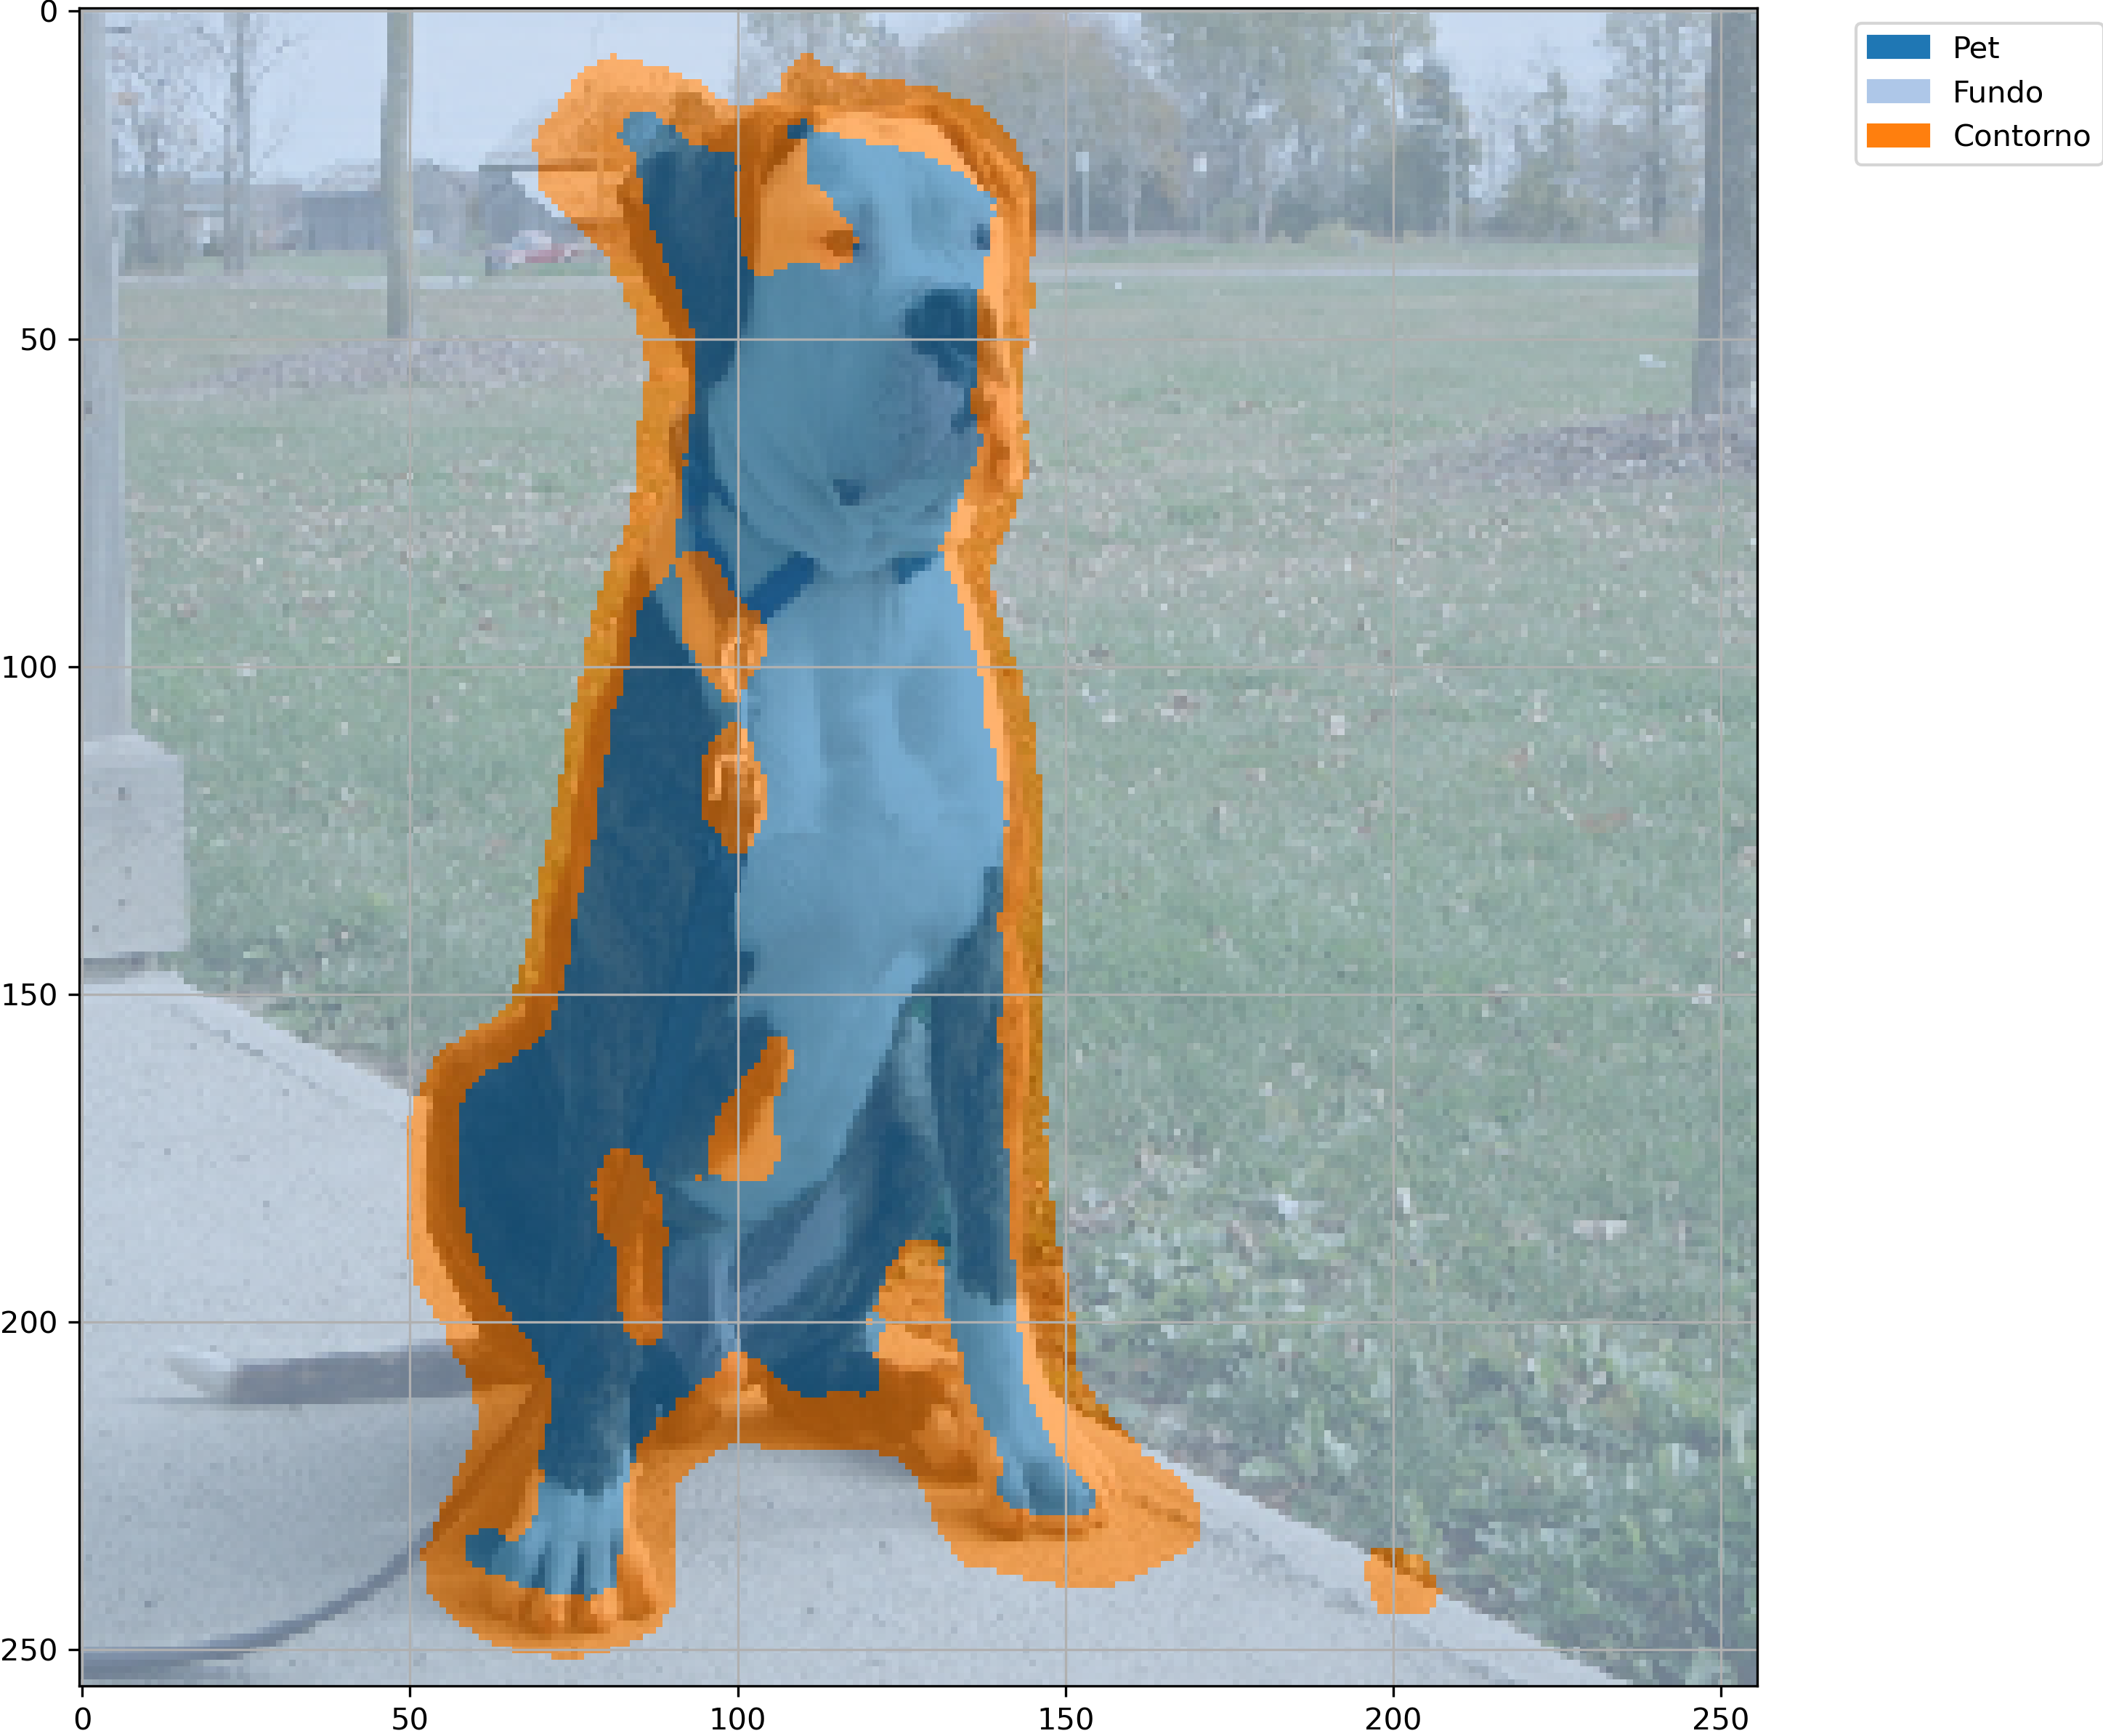
\includegraphics[width=1\linewidth]{recursos/imagens/results/bpca_miou_unet500_image_2_overlayed_segmentation.png}
         \label{results:fig:semantic:3.2}
     \end{subfigure}%

    Fonte: do próprio autor.
\end{figure}

\begin{figure}[H]
    \centering
    \caption{Exemplos segmentados a partir de U-Net com \textit{Max Pooling} e 500 épocas no conjunto de dados \textit{Oxford-IIIT Pets} baseada em acurácia.}
    \label{results:fig:semantic:4}
     \begin{subfigure}[t]{0.32\textwidth}
         \centering
         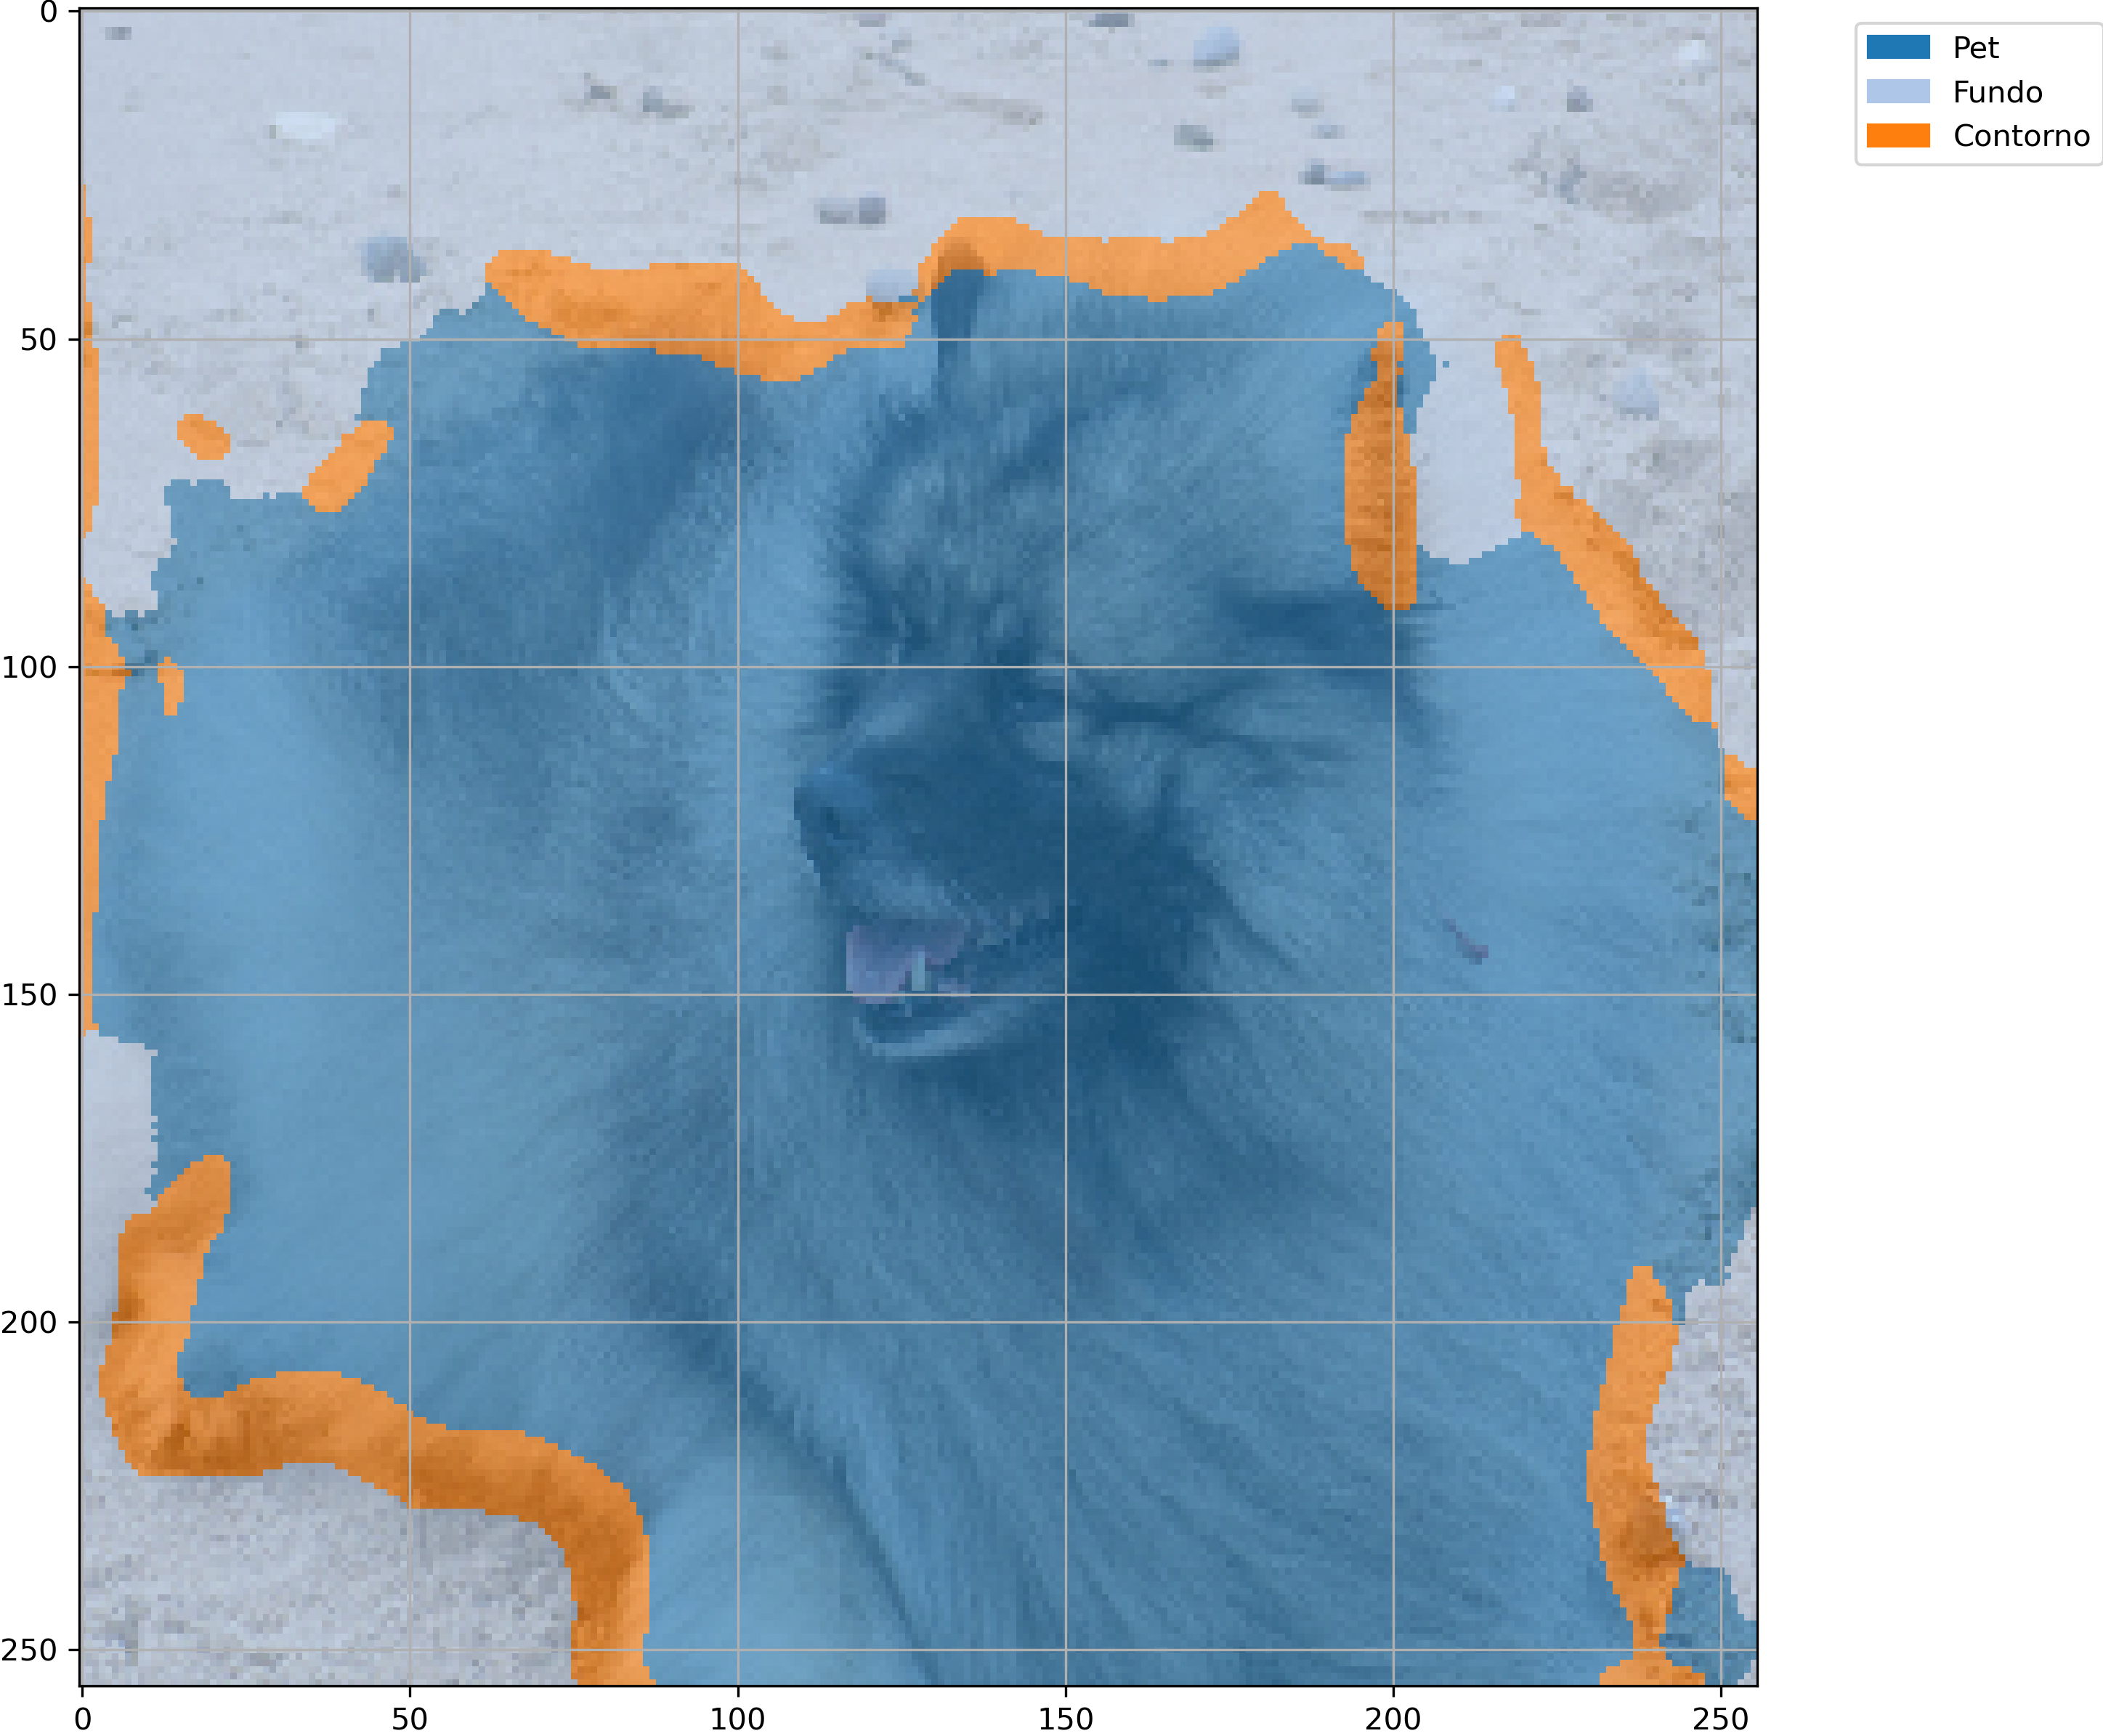
\includegraphics[width=1\linewidth]{recursos/imagens/results/max_acc_unet500_image_0_overlayed_segmentation.png}
         \label{results:fig:semantic:4.1}
     \end{subfigure}%
     ~ 
     \begin{subfigure}[t]{0.32\textwidth}
         \centering
         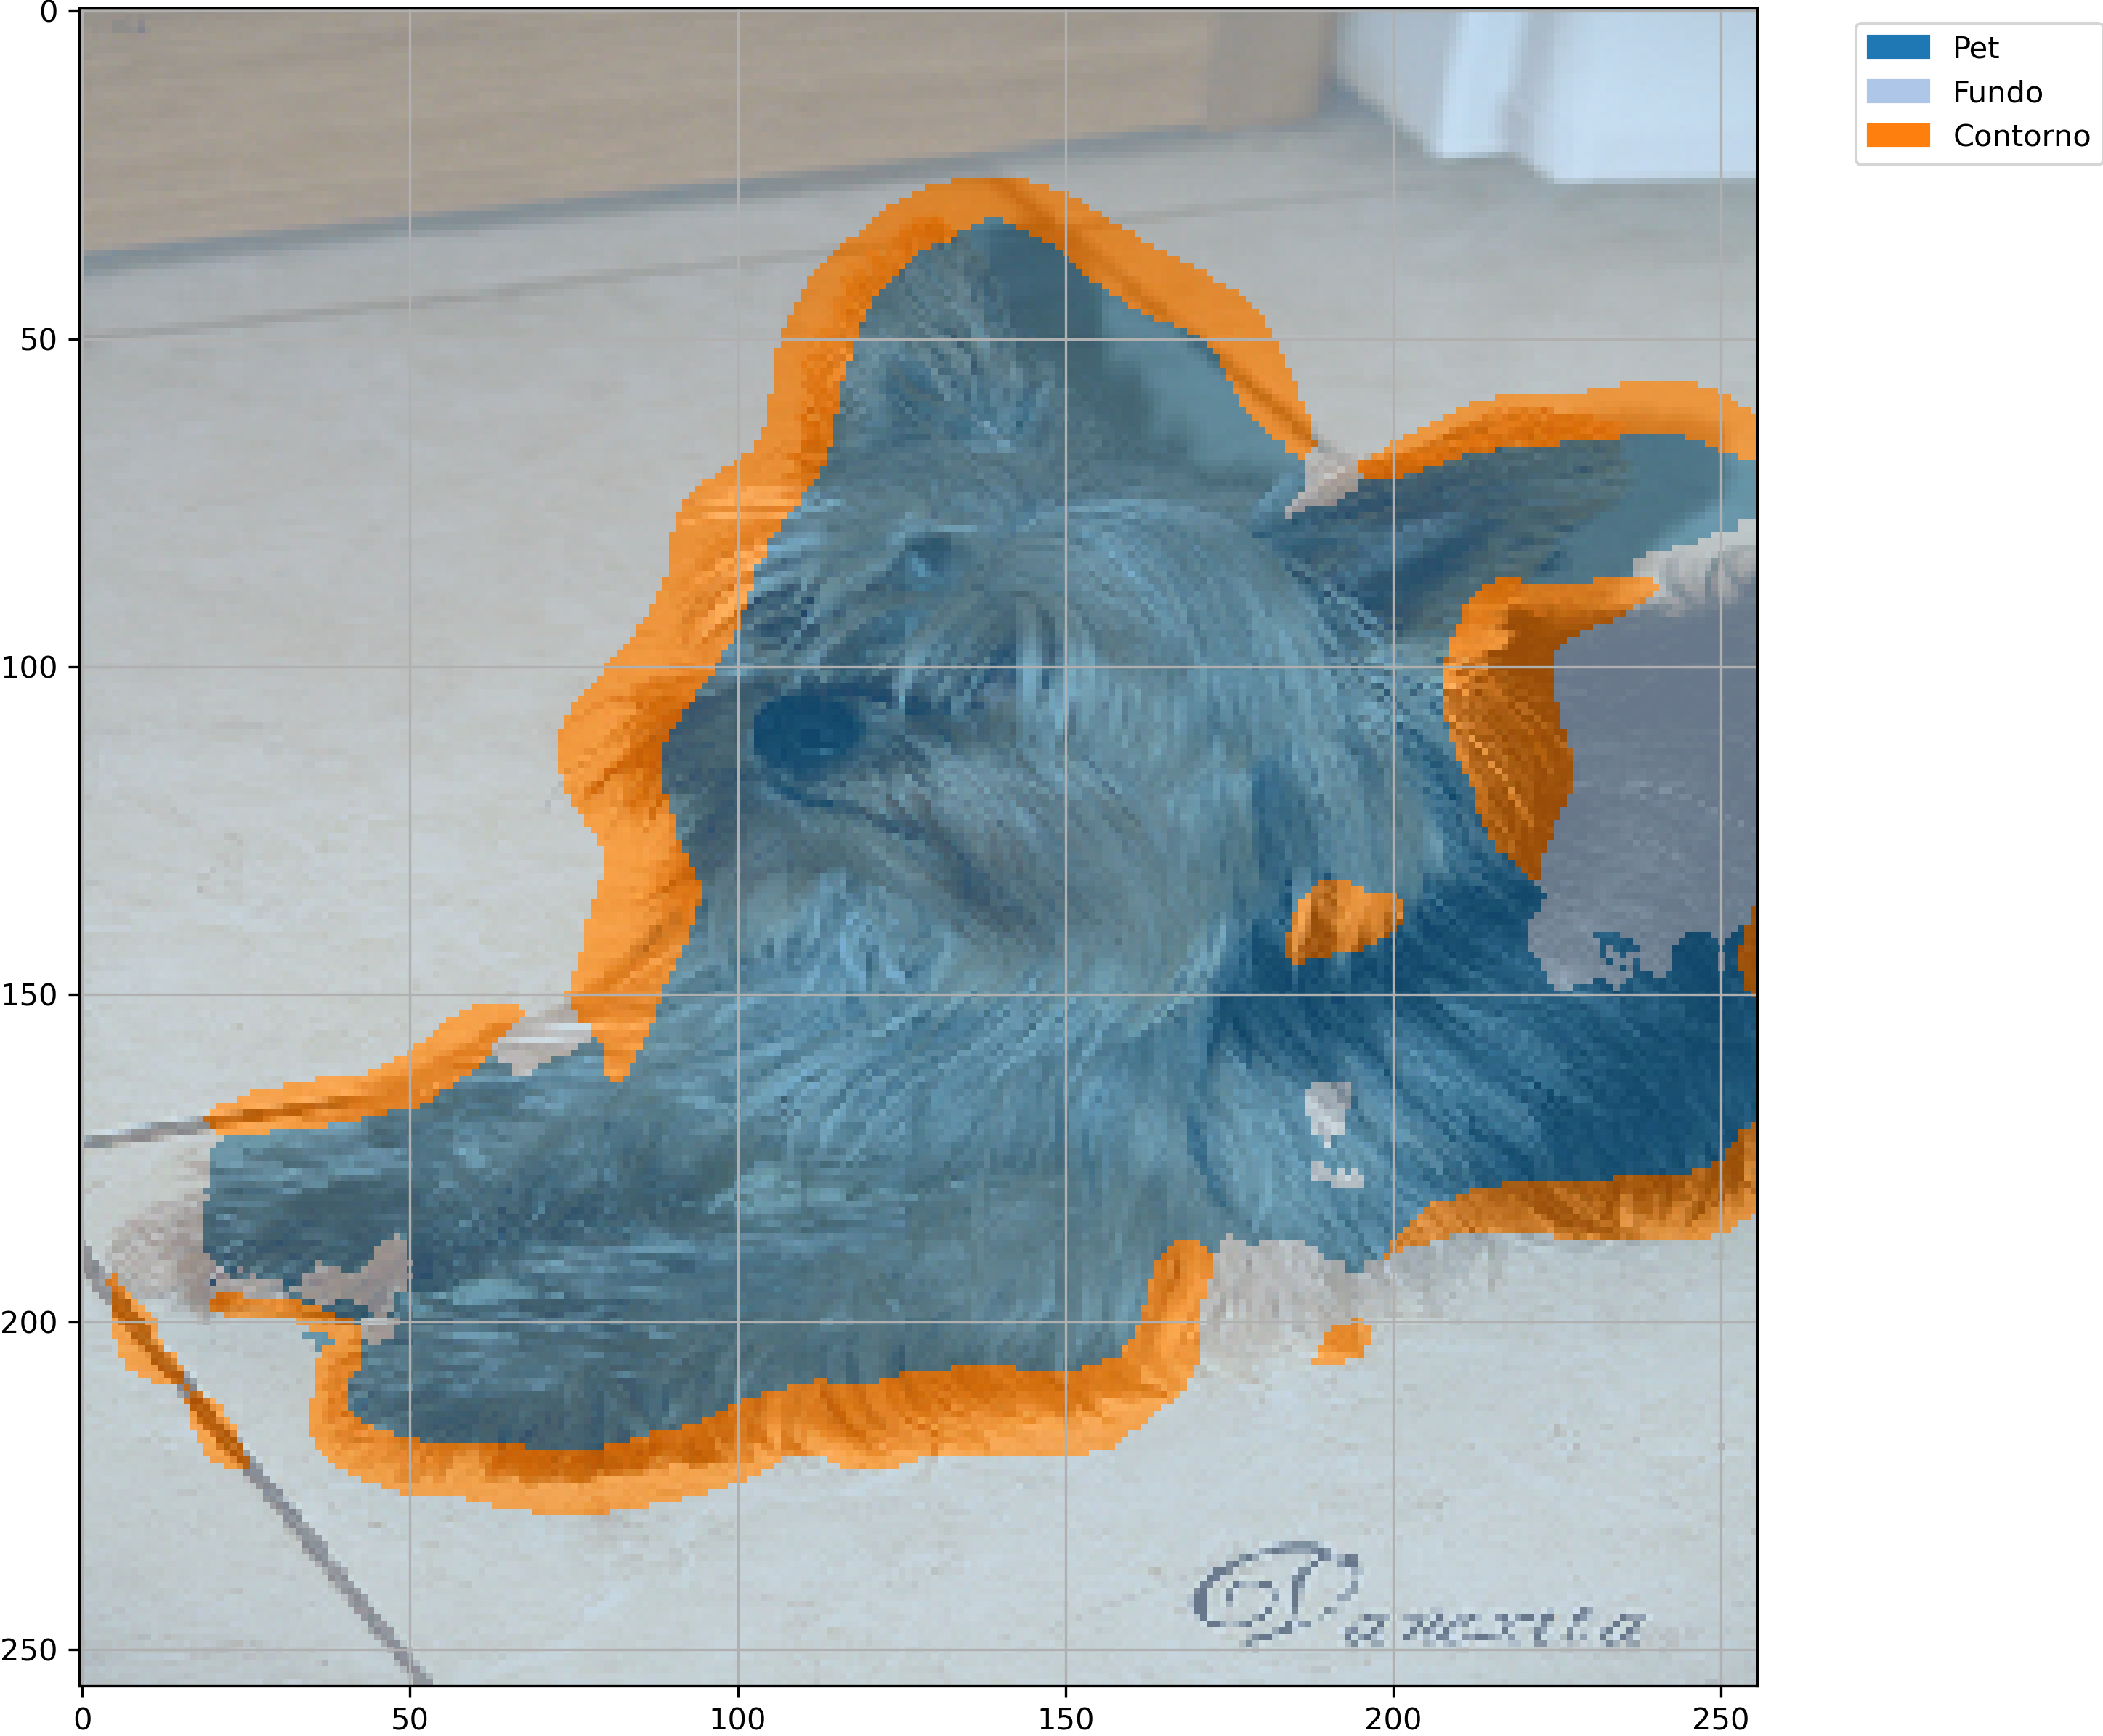
\includegraphics[width=1\linewidth]{recursos/imagens/results/max_acc_unet500_image_1_overlayed_segmentation.png}
         \label{results:fig:semantic:4.2}
     \end{subfigure}%
     ~ 
    \begin{subfigure}[t]{0.32\textwidth}
         \centering
         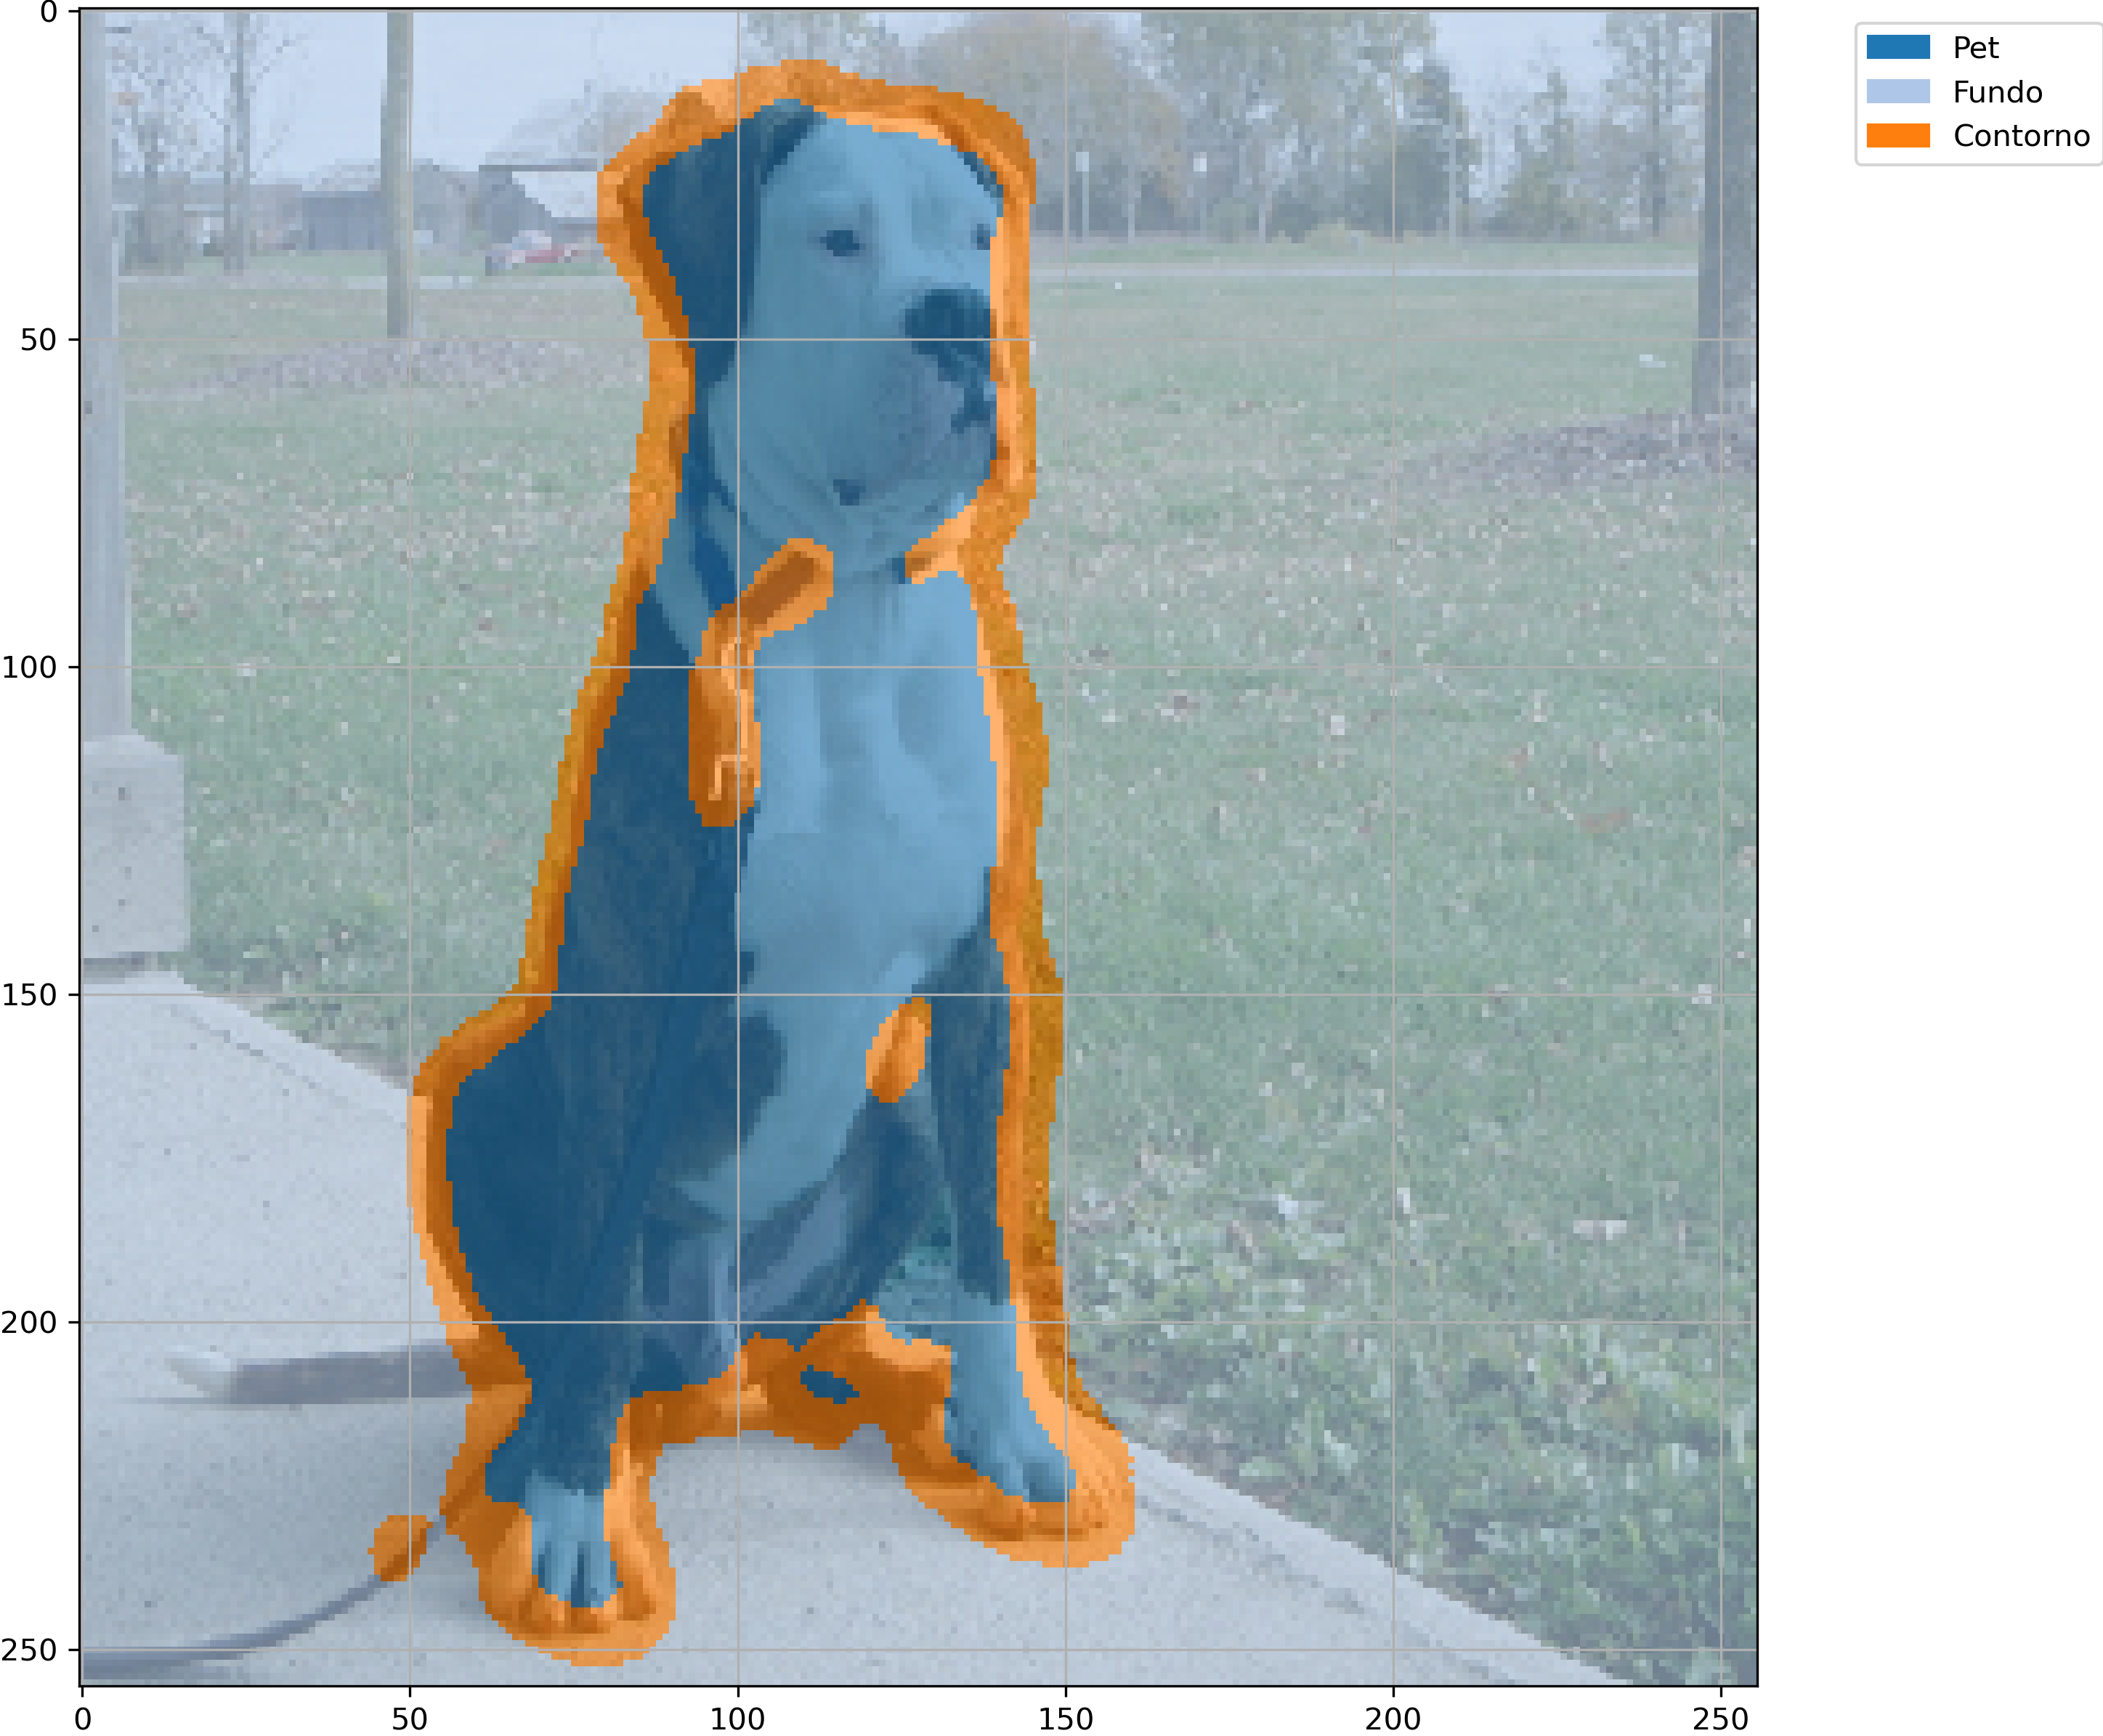
\includegraphics[width=1\linewidth]{recursos/imagens/results/max_acc_unet500_image_2_overlayed_segmentation.png}
         \label{results:fig:semantic:4.2}
     \end{subfigure}%

    Fonte: do próprio autor.
\end{figure}

\begin{figure}[H]
    \centering
    \caption{Exemplos segmentados a partir de U-Net com BPCAPooling e 500 épocas no conjunto de dados \textit{Oxford-IIIT Pets} baseada em acurácia.}
    \label{results:fig:semantic:5}
     \begin{subfigure}[t]{0.32\textwidth}
         \centering
         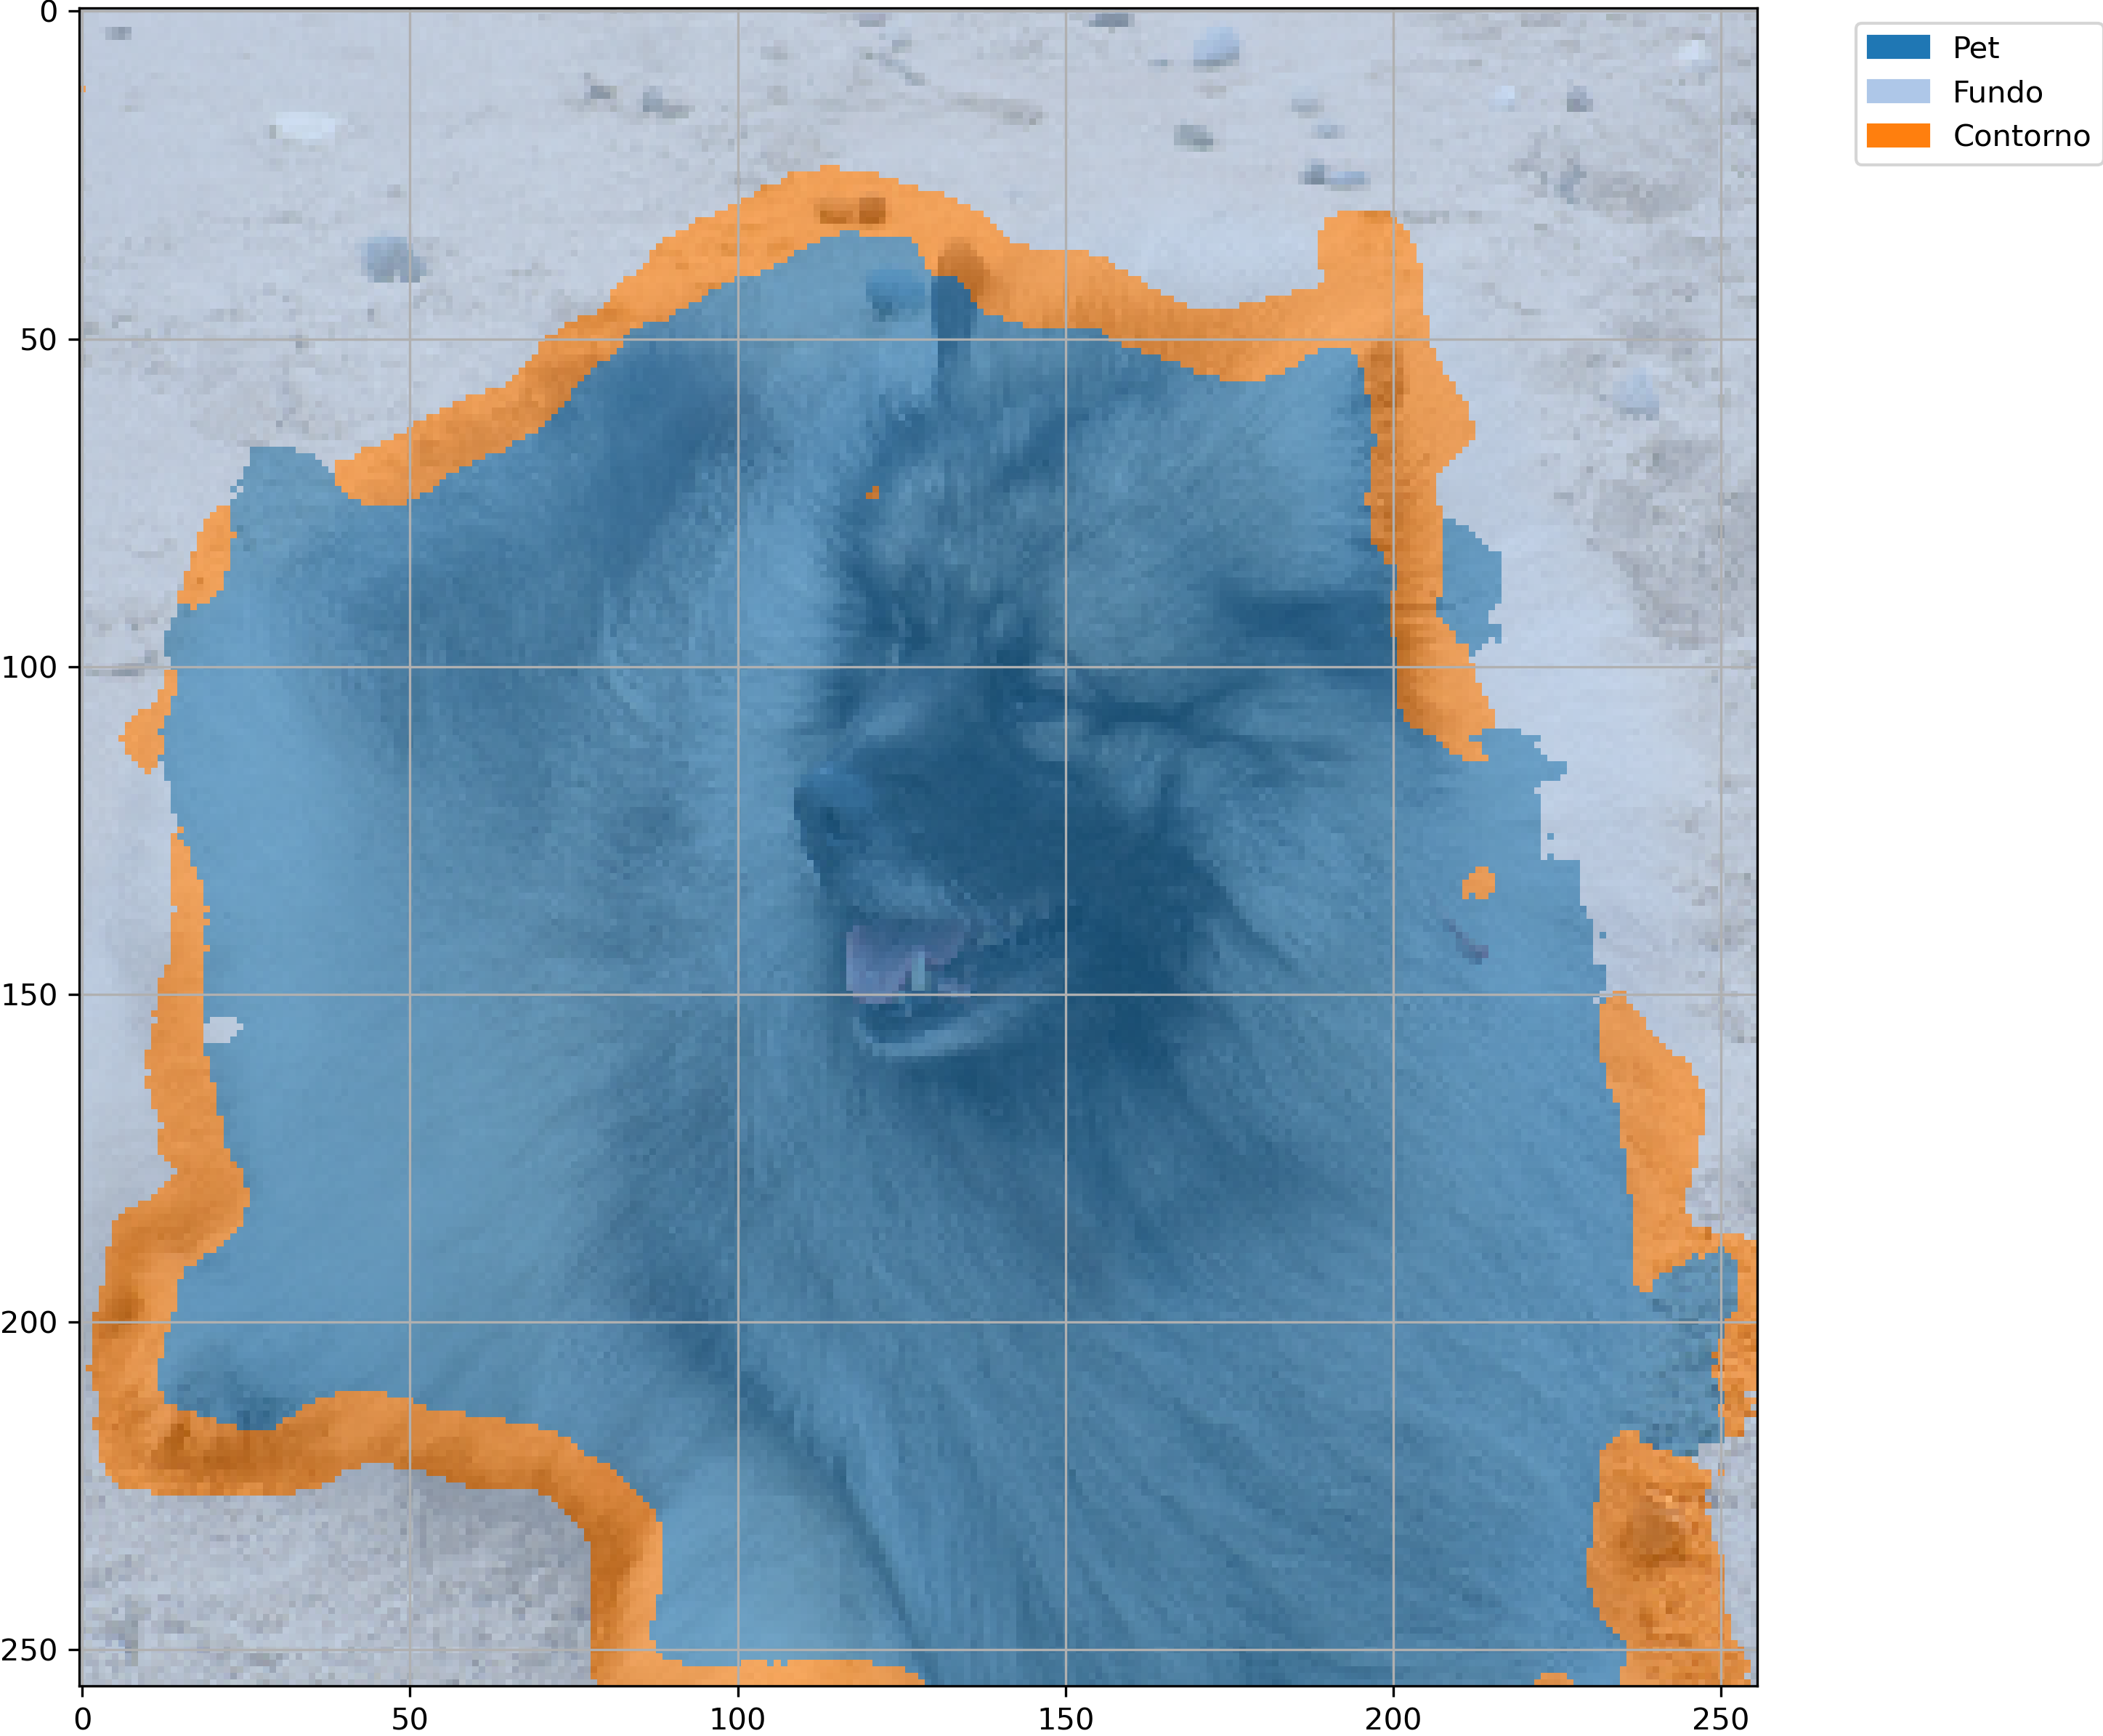
\includegraphics[width=1\linewidth]{recursos/imagens/results/bpca_acc_unet500_image_0_overlayed_segmentation.png}
         \label{results:fig:semantic:5.1}
     \end{subfigure}%
     ~ 
     \begin{subfigure}[t]{0.32\textwidth}
         \centering
         \includegraphics[width=1\linewidth]{recursos/imagens/results/bpca_acc_unet500_image_1_overlayed_segmentation.png}
         \label{results:fig:semantic:5.2}
     \end{subfigure}%
     ~ 
    \begin{subfigure}[t]{0.32\textwidth}
         \centering
         \includegraphics[width=1\linewidth]{recursos/imagens/results/bpca_acc_unet500_image_2_overlayed_segmentation.png}
         \label{results:fig:semantic:5.2}
     \end{subfigure}%

    Fonte: do próprio autor.
\end{figure}

Os resultados obtidos com a arquitetura U-Net-\textit{Like} não apresentaram grandes diferenças quando comparados com os casos anteriores ou com a utilização do método \textit{Max Pooling}. No entanto, é importante ressaltar que, ao empregar a U-Net-\textit{Like}, os resultados do BPCAPooling mostraram-se inferiores em todos os aspectos, exceto nos valores de Dice na etapa de validação, como também ocorreu na arquitetura U-Net. Essa comparação é ilustrada nas Tabelas \ref{results:semantic:tab:3} e \ref{results:semantic:tab:4}.

\begin{table}[H]
    \centering
    \caption{Resultados de U-Net-\textit{Likes} treinadas por 500 épocas no conjunto de dados \textit{Oxford-IIIT Pets} com base em acurácia.}
    \label{results:semantic:tab:3}
    \resizebox{1\textwidth}{!}{
        \begin{tabular}{l|l|l|l|l|l}
            \multicolumn{1}{c|}{\textbf{Método de \textit{Pooling}}} & \multicolumn{1}{c|}{\textbf{Tempo de Execução}}  & \multicolumn{2}{c|}{\textbf{Acurácia (\%)}}                                    & \multicolumn{2}{c}{\textbf{\textit{Loss}}}                                    \\
            \cline{3-6}
            \multicolumn{1}{c|}{}                                    & \multicolumn{1}{c|}{\textbf{(minutos)}}          & \multicolumn{1}{c|}{\textbf{Treino}} & \multicolumn{1}{c|}{\textbf{Validação}} & \multicolumn{1}{c|}{\textbf{Treino}} & \multicolumn{1}{c}{\textbf{Validação}} \\
            \hline
            BPCAPooling                                              &  116:99                                         &  79,312                               &  78,61                                  &  0,7032                              &  0,8109                                \\
            \textit{Max Pooling}                                     &  \textbf{24:81}                                 &  \textbf{82,472}                      &  \textbf{81,84}                         &  \textbf{0.6144}                     &  \textbf{0,7936}                       \\
        \end{tabular}
    }

    \vspace*{1 cm}
    Fonte: do próprio autor.
\end{table}

\begin{table}[H]
    \centering
    \caption{Resultados de U-Net-\textit{Likes} treinadas por 20 épocas no conjunto de dados \textit{Oxford-IIIT Pets} com base em mIoU.}
    \label{results:semantic:tab:4}
    \resizebox{1\textwidth}{!}{
        \begin{tabular}{l|l|l|l|l|l|l|l|l|l}
            \multicolumn{1}{c|}{\textbf{Método de \textit{Pooling}}} & \multicolumn{1}{c|}{\textbf{Tempo de Execução}}  & \multicolumn{2}{c|}{\textbf{Acurácia (\%)}}                                    & \multicolumn{2}{c|}{\textbf{\textit{Loss}}}                                    & \multicolumn{2}{c|}{\textbf{mIoU}}                                             & \multicolumn{2}{c}{\textbf{Dice}}                                               \\
            \cline{3-10}
            \multicolumn{1}{c|}{}                                    & \multicolumn{1}{c|}{\textbf{(minutos)}}          & \multicolumn{1}{c|}{\textbf{Treino}} & \multicolumn{1}{c|}{\textbf{Validação}} & \multicolumn{1}{c|}{\textbf{Treino}} & \multicolumn{1}{c|}{\textbf{Validação}}  & \multicolumn{1}{c|}{\textbf{Treino}} & \multicolumn{1}{c|}{\textbf{Validação}} & \multicolumn{1}{c|}{\textbf{Treino}} & \multicolumn{1}{c}{\textbf{Validação}}  \\
            \hline
            BPCAPooling                                              &  10.99                                           &  70,95                               &  71,55                                  &  0,7133                              &  0,6935                                 & 0,3086                               & 0,3102                                  & \textbf{0,8889}                               & 0,8970                                   \\
            \textit{Max Pooling}                                     &  \textbf{3:19}                                   &  \textbf{77,97}                      &  \textbf{78,19}                         &  \textbf{0,5571}                     &  \textbf{0,5508}                                 & \textbf{0,3164}                      & \textbf{0,3177}                         & 0,8892                                        & 0,8970                                   \\
        \end{tabular}
    }

    \vspace*{1 cm}
    Fonte: do próprio autor.
\end{table}

Além da métrica Dice, vale ressaltar que o comportamento do tempo de execução é muito semelhante ao observado nos casos de uso das U-Nets, em que as abordagens com \textit{Max Pooling} demonstram um melhor desempenho. Contudo, ao comparar os tempos de execução da Tabela \ref{results:semantic:tab:3} com as Tabelas \ref{results:semantic:tab:1} e \ref{results:semantic:tab:2}, nota-se que o desempenho das U-Net-\textit{Like} é superior. Isso se deve à influência das estratégias de otimização, como normalização de \textit{batch}, convolução separável e \textit{upsampling}, que reduzem a quantidade de parâmetros em comparação com as U-Nets convencionais. No entanto, as comparações em relação aos valores de avaliação ainda se mostram superiores nas U-Nets convencionais, demonstrando que a robustez da arquitetura original tem seus benefícios.

A Figura \ref{results:fig:semantic:6} ilustra o progresso das métricas durante o processo de treinamento e validação dos modelos de U-Net-\textit{Like}, guiados pela métrica de acurácia. Já as Figuras \ref{results:fig:semantic:7} e \ref{results:fig:semantic:8} mostram os resultados dos modelos U-Net-\textit{Like} treinados por menos épocas, mas que apresentam métricas mais apropriadas para o contexto de segmentação semântica.

\begin{figure}[H]
    \centering
    \caption{Métricas de U-Net-\textit{Likes} com 500 épocas no conjunto de dados \textit{Oxford-IIIT Pets} baseada em acurácia.}
    \label{results:fig:semantic:6}
     \begin{subfigure}[t]{0.45\textwidth}
         \centering
         \includegraphics[width=1\linewidth]{recursos/imagens/results/max500_ulike_acc_accuracy.png}
         \caption{Acurácia do \textit{Max Pooling}.}
         \label{results:fig:semantic:6.1}
     \end{subfigure}%
     ~ 
     \begin{subfigure}[t]{0.45\textwidth}
         \centering
         \includegraphics[width=1\linewidth]{recursos/imagens/results/max500_ulike_acc_loss.png}
         \caption{\textit{Loss} do \textit{Max Pooling}.}
         \label{results:fig:semantic:6.2}
     \end{subfigure}%
     ~ 
     
     \begin{subfigure}[t]{0.45\textwidth}
         \centering
         \includegraphics[width=1\linewidth]{recursos/imagens/results/bpca500_ulike_acc_accuracy.png}
         \caption{Acurácia do BPCAPooling.}
         \label{results:fig:semantic:6.3}
     \end{subfigure}
     ~
     \begin{subfigure}[t]{0.45\textwidth}
         \centering
         \includegraphics[width=1\linewidth]{recursos/imagens/results/bpca500_ulike_acc_loss.png}
         \caption{\textit{Loss} do BPCAPooling.}
         \label{results:fig:semantic:6.4}
     \end{subfigure}
     
     Fonte: do próprio autor.
\end{figure}

\begin{figure}[H]
    \centering
    \caption{Métricas de U-Net-\textit{Likes} com BPCAPooling e 20 épocas no conjunto de dados \textit{Oxford-IIIT Pets} baseada em mIoU.}
    \label{results:fig:semantic:7}
     \begin{subfigure}[t]{0.45\textwidth}
         \centering
         \includegraphics[width=1\linewidth]{recursos/imagens/results/bpca_unetlike20_miou_accuracy.png}
         \caption{Acurácia.}
         \label{results:fig:semantic:7.1}
     \end{subfigure}%
     ~ 
     \begin{subfigure}[t]{0.45\textwidth}
         \centering
         \includegraphics[width=1\linewidth]{recursos/imagens/results/bpca_unetlike20_miou_loss.png}
         \caption{\textit{Loss}.}
         \label{results:fig:semantic:7.2}
     \end{subfigure}%
     ~ 
     
     \begin{subfigure}[t]{0.45\textwidth}
         \centering
         \includegraphics[width=1\linewidth]{recursos/imagens/results/bpca_unetlike20_miou_dice_coefficient.png}
         \caption{Dice.}
         \label{results:fig:semantic:7.3}
     \end{subfigure}
     ~
     \begin{subfigure}[t]{0.45\textwidth}
         \centering
         \includegraphics[width=1\linewidth]{recursos/imagens/results/bpca_unetlike20_miou_mean_iou.png}
         \caption{mIoU.}
         \label{results:fig:semantic:7.4}
     \end{subfigure}
     
     Fonte: do próprio autor.
\end{figure}

\begin{figure}[H]
    \centering
    \caption{Métricas de U-Net-\textit{Likes} com \textit{Max Pooling} e 20 épocas no conjunto de dados \textit{Oxford-IIIT Pets} baseada em mIoU.}
    \label{results:fig:semantic:8}
     \begin{subfigure}[t]{0.45\textwidth}
         \centering
         \includegraphics[width=1\linewidth]{recursos/imagens/results/max_unetlike20_miou_accuracy.png}
         \caption{Acurácia.}
         \label{results:fig:semantic:8.1}
     \end{subfigure}%
     ~ 
     \begin{subfigure}[t]{0.45\textwidth}
         \centering
         \includegraphics[width=1\linewidth]{recursos/imagens/results/max_unetlike20_miou_loss.png}
         \caption{\textit{Loss}.}
         \label{results:fig:semantic:8.2}
     \end{subfigure}%
     ~ 
     
     \begin{subfigure}[t]{0.45\textwidth}
         \centering
         \includegraphics[width=1\linewidth]{recursos/imagens/results/max_unetlike20_miou_dice_coefficient.png}
         \caption{Dice.}
         \label{results:fig:semantic:8.3}
     \end{subfigure}
     ~
     \begin{subfigure}[t]{0.45\textwidth}
         \centering
         \includegraphics[width=1\linewidth]{recursos/imagens/results/max_unetlike20_miou_mean_iou.png}
         \caption{mIoU.}
         \label{results:fig:semantic:8.4}
     \end{subfigure}
     
     Fonte: do próprio autor.
\end{figure}

Analisando essas tabelas por meio de testes estatísticos, observa-se uma diferença estatisticamente significativa para as métricas de acurácia e \textit{loss} nas fases de treinamento e validação das U-Net-\textit{Like} baseadas na acurácia, considerando um nível de significância de $5\%$. No entanto, essa diferença não é observada para as demais métricas, como Dice, acurácia de validação, Dice de validação, \textit{loss} de validação e mIoU de validação, apresentando os respectivos valores de p-valor de $0.7962$, $0.6730$, $0.2130$, $0.1175$ e $0.2198$, ainda mantendo o limiar de significância de $5\%$.

Em termos visuais, assim como constatado anteriormente com as U-Nets, além da análise das métricas, as imagens também indicam uma qualidade inferior na segmentação em comparação com os modelos U-Net. As Figuras \ref{results:fig:semantic:9} e \ref{results:fig:semantic:10} exibem as imagens de entrada, as máscaras e as máscaras geradas pelo modelo para um melhor entendimento visual.

\begin{figure}[H]
    \centering
   \caption{Imagem de entrada, máscara e saída do modelo U-Net-\textit{Like} baseado em acurácia, respectivamente.}
    \label{results:fig:semantic:9}
    \begin{subfigure}[t]{0.9\textwidth}
        \centering
        \includegraphics[width=1\linewidth]{recursos/imagens/results/image_0_max_unetlike_500.png}
        \caption{Modelo com \textit{Max Pooling}.}
        \label{results:fig:semantic:9.1}
    \end{subfigure}%
    ~
    
    \begin{subfigure}[t]{0.9\textwidth}
        \centering
        \includegraphics[width=1\linewidth]{recursos/imagens/results/image_0_bpca_unetlike_500.png}
        \caption{Modelo com BPCAPooling.}
        \label{results:fig:semantic:9.2}
    \end{subfigure}%

    Fonte: do próprio autor.
\end{figure}

\begin{figure}[H]
    \centering
   \caption{Imagem de entrada, máscara e saída do modelo U-Net-\textit{Like} baseado em mIoU, respectivamente.}
    \label{results:fig:semantic:10}
    \begin{subfigure}[t]{0.9\textwidth}
        \centering
        \includegraphics[width=1\linewidth]{recursos/imagens/results/image_0_max_unetlike_miou.png}
        \caption{Modelo com \textit{Max Pooling}.}
        \label{results:fig:semantic:10.1}
    \end{subfigure}%
    ~
    
    \begin{subfigure}[t]{1\textwidth}
        \centering
        \includegraphics[width=0.9\linewidth]{recursos/imagens/results/image_0_bpca_unetlike_miou.png}
        \caption{Modelo com BPCAPooling.}
        \label{results:fig:semantic:10.2}
    \end{subfigure}%

    Fonte: do próprio autor.
\end{figure}

Por fim, ao analisar as Figuras \ref{results:fig:semantic:11}, \ref{results:fig:semantic:12}, \ref{results:fig:semantic:13} e \ref{results:fig:semantic:14}, evidencia-se a sobreposição dos resultados do modelo nas imagens de entrada. Esta visualização sinaliza a necessidade de estender o número de épocas para os modelos de segmentação U-Net-\textit{Like} treinados por apenas 20 épocas. Apesar da diferença nas acurácias não exceder $8\%$, a análise visual sugere um potencial de melhoria substancial, indicando que o modelo possivelmente pode obter resultados mais robustos com um treinamento prolongado.

\begin{figure}[H]
    \centering
    \caption{Exemplos segmentados a partir de U-Net-\textit{Like} com \textit{Max Pooling} e 500 épocas no conjunto de dados \textit{Oxford-IIIT Pets} baseada em acurácia.}
    \label{results:fig:semantic:11}
     \begin{subfigure}[t]{0.32\textwidth}
         \centering
         \includegraphics[width=1\linewidth]{recursos/imagens/results/max_acc_unetlike500_image_0_overlayed_segmentation.png}
         \label{results:fig:semantic:11.1}
     \end{subfigure}%
     ~ 
     \begin{subfigure}[t]{0.32\textwidth}
         \centering
         \includegraphics[width=1\linewidth]{recursos/imagens/results/max_acc_unetlike500_image_1_overlayed_segmentation.png}
         \label{results:fig:semantic:11.2}
     \end{subfigure}%
     ~ 
    \begin{subfigure}[t]{0.32\textwidth}
         \centering
         \includegraphics[width=1\linewidth]{recursos/imagens/results/max_acc_unetlike500_image_2_overlayed_segmentation.png}
         \label{results:fig:semantic:11.2}
     \end{subfigure}%

    Fonte: do próprio autor.
\end{figure}

\begin{figure}[H]
    \centering
    \caption{Exemplos segmentados a partir de U-Net-\textit{Like} com BPCAPooling e 500 épocas no conjunto de dados \textit{Oxford-IIIT Pets} baseada em acurácia.}
    \label{results:fig:semantic:12}
     \begin{subfigure}[t]{0.32\textwidth}
         \centering
         \includegraphics[width=1\linewidth]{recursos/imagens/results/bpca_acc_unetlike500_image_0_overlayed_segmentation.png}
         \label{results:fig:semantic:12.1}
     \end{subfigure}%
     ~ 
     \begin{subfigure}[t]{0.32\textwidth}
         \centering
         \includegraphics[width=1\linewidth]{recursos/imagens/results/bpca_acc_unetlike500_image_1_overlayed_segmentation.png}
         \label{results:fig:semantic:12.2}
     \end{subfigure}%
     ~ 
    \begin{subfigure}[t]{0.32\textwidth}
         \centering
         \includegraphics[width=1\linewidth]{recursos/imagens/results/bpca_acc_unetlike500_image_2_overlayed_segmentation.png}
         \label{results:fig:semantic:12.2}
     \end{subfigure}%

    Fonte: do próprio autor.
\end{figure}

\begin{figure}[H]
    \centering
    \caption{Exemplos segmentados a partir de U-Net-\textit{Like} com \textit{Max Pooling} e 20 épocas no conjunto de dados \textit{Oxford-IIIT Pets} baseada em mIoU.}
    \label{results:fig:semantic:13}
     \begin{subfigure}[t]{0.32\textwidth}
         \centering
         \includegraphics[width=1\linewidth]{recursos/imagens/results/max_miou_unetlike500_image_0_overlayed_segmentation.png}
         \label{results:fig:semantic:13.1}
     \end{subfigure}%
     ~ 
     \begin{subfigure}[t]{0.32\textwidth}
         \centering
         \includegraphics[width=1\linewidth]{recursos/imagens/results/max_miou_unetlike500_image_1_overlayed_segmentation.png}
         \label{results:fig:semantic:13.2}
     \end{subfigure}%
     ~ 
    \begin{subfigure}[t]{0.32\textwidth}
         \centering
         \includegraphics[width=1\linewidth]{recursos/imagens/results/max_miou_unetlike500_image_2_overlayed_segmentation.png}
         \label{results:fig:semantic:13.2}
     \end{subfigure}%

    Fonte: do próprio autor.
\end{figure}

\begin{figure}[H]
    \centering
    \caption{Exemplos segmentados a partir de U-Net-\textit{Like} com BPCAPooling e 20 épocas no conjunto de dados \textit{Oxford-IIIT Pets} baseada em mIoU.}
    \label{results:fig:semantic:14}
     \begin{subfigure}[t]{0.32\textwidth}
         \centering
         \includegraphics[width=1\linewidth]{recursos/imagens/results/bpca_miou_unetlie500_image_0_overlayed_segmentation.png}
         \label{results:fig:semantic:14.1}
     \end{subfigure}%
     ~ 
     \begin{subfigure}[t]{0.32\textwidth}
         \centering
         \includegraphics[width=1\linewidth]{recursos/imagens/results/bpca_miou_unetlie500_image_1_overlayed_segmentation.png}
         \label{results:fig:semantic:14.2}
     \end{subfigure}%
     ~ 
    \begin{subfigure}[t]{0.32\textwidth}
         \centering
         \includegraphics[width=1\linewidth]{recursos/imagens/results/bpca_miou_unetlie500_image_2_overlayed_segmentation.png}
         \label{results:fig:semantic:14.2}
     \end{subfigure}%

    Fonte: do próprio autor.
\end{figure}



\subsubsection{Explicação de modelos}
\label{results:semantic:xai}
- Colocar o grafo para cada um dos modelos e mostra apenas as imagens de destaque
    - UNet 500 + BPCA (3 imagens + 1 grafo)
    - UNet 500 + MaxPooling (3 imagens + 1 grafo)
    - UNet Like 20 + BPCA (3 imagens + 1 grafo)
    - UNet Like 20 + MaxPooling (3 imagens + 1 grafo)

\subsubsection{Trabalhos Futuros}
\label{results:semantic:future}
Para contribuir com o avanço deste projeto, esta seção propõe identificar pontos de melhoria e desafios encontrados para a aplicação mais ampla e aprimoramento do BPCAPooling. O objetivo é potencializar seu desempenho em relação aos métodos tradicionais, não apenas reduzindo a dimensionalidade de entradas em arquiteturas de segmentação semântica, mas também preservando a espacialidade dessas informações.

Um dos grandes desafios encontrados residia na combinação dos \textit{frameworks} Tensorflow e Keras. Dado que a abordagem proposta consistia no desenvolvimento de uma camada personalizada de \textit{pooling}, erros de desenvolvimento eram comuns, afetando significativamente o tempo de implementação e outros aspectos mencionados nesta seção. Portanto, uma proposta para futuros trabalhos seria a exploração de diferentes \textit{frameworks}, como PyTorch \citep{Paszke2017AutomaticPyTorch}. Além de potencialmente melhorar o desempenho do método, conforme discutido na Seção \ref{results:class:future}.

A dificuldade enfrentada com o \textit{framework} também prejudicou a aplicação do método em mais de um conjunto de dados para a tarefa de segmentação semântica. Uma excelente proposta futura seria estender os testes para um segundo conjunto de dados, preferencialmente com múltiplos objetos de interesse em cada exemplo. Conjuntos como \textit{Cityscape} \citep{Cordts2016} e \textit{Lost and Found} \citep{Pinggera2016LostVehicles} oferecem condições ideais para avaliar as capacidades de preservação de espacialidade do BPCAPooling em cenários mais complexos.

Além disso, iniciou-se o desenvolvimento do método BPCAUnpooling, disponível no repositório do projeto \footnote{Repositório Github do projeto - \url{https://github.com/Lucs1590/USeS-BPCA}}, mas a implementação com o \textit{framework} atual representou uma barreira. Esse método seria uma abordagem de \textit{unpooling}, contrapartida ao BPCAPooling, revertendo o processo proposto por este último, preservando também a espacialidade no processo de reconstrução realizado pelas U-Nets e similares, como ilustrado na Figura \ref{results:fig:future:0}.

\begin{figure}[H]
    \centering
    \caption{Processo de redução e reconstrução de dimensionalidade com BPCAPooling e BPCAUnpooling, respectivamente.}
    \label{results:fig:future:0}
    \includegraphics[width=1\textwidth]{recursos/imagens/results/bpca_unpooling.png}

    Fonte: do próprio autor.
\end{figure}

Ao contrário do BPCAPooling, a aplicação do método BPCAUnpooling requer camadas densas para alcançar um comportamento equivalente ao das camadas transpostas. A Equação \ref{results:eq:bpca_unpooling} ilustra esse método, onde $X'_{i,j,k}$ representa o mapa de características de saída com dimensões correspondentes à altura ($i$), largura ($j$) e canais ($k$). Essa equação descreve o processo de reconstrução da dimensionalidade usando o método BPCAUnpooling, que envolve operações de preenchimento, remodelagem e reconstrução dos dados não agrupados por meio da decomposição PCA.

\begin{equation}
    \label{results:eq:bpca_unpooling}
    \begin{split}
        X'_{i,j,k} &= \text{BPCAUnpooling}(Y_{i',j',k'}) \\
                  &= \text{reshape}\left(U \cdot \left(\text{reshape}(S) \cdot \text{Dense}\left(\text{pad}(Y)\right)\right)\right) \cdot {\sigma} + {\mu}.
    \end{split}
\end{equation}

Nesta equação, o parâmetro $\text{BPCAUnpooling}(Y_{i',j',k'})$ representa a aplicação do método BPCAUnpooling ao mapa de características de entrada $Y$. A função $pad(Y)$ preenche o mapa de características de entrada $Y$ com zeros para ajustar o tamanho necessário para a operação de \textit{unpooling}, enquanto $Dense(pad(Y))$ é utilizado para aprender os componentes do PCA, empregando uma camada densa com ativação. A função $\text{reshape}$, como no processo da equação \ref{project:eq:bpca}, remodela os argumentos para o tamanho correto, onde $S$ representa os valores singulares da decomposição PCA alinhados com os componentes PCA. A expressão $U \cdot (reshape(S) \cdot Dense(pad(Y)))$ reconstrói os dados não agrupados utilizando os componentes e valores singulares do PCA. Por fim, a multiplicação pelo desvio padrão ($\sigma$) e a adição da média ($\mu$) revertem a transformação PCA.

\subsection{Considerações Finais do Capítulo}
\label{result:final}
Neste capítulo, foram apresentados os resultados dos experimentos realizados, abordando tanto o processo de classificação (Seção \ref{results:class}) quanto os primeiros passos em direção ao objetivo final de empregar o BPCAPooling como uma proposta de camada de \textit{pooling} para segmentações semânticas, como explorado e detalhado na Seção \ref{results:semantic}. Além disso, foram delineadas ideias para melhorias e desenvolvimento futuro nestas áreas, destacadas nas Seções \ref{results:class:future} e \ref{results:semantic:future}.

No próximo capítulo, as conclusões derivadas deste trabalho serão discutidas, demonstrando a efetividade do método proposto em relação à sua aplicabilidade e ao alcance dos objetivos estabelecidos no início deste estudo (Seção \ref{intro:objectives}).